
\documentclass[11pt,a4paper]{article}

\usepackage[T1]{fontenc}
\usepackage{lmodern}
\usepackage[margin=2.6cm]{geometry}
\usepackage{amsmath,amssymb,bm}
\usepackage{booktabs}
\usepackage{longtable}
\usepackage{array}
\usepackage{graphicx}
\usepackage{xcolor}
\usepackage{listings}
\usepackage{microtype}
\usepackage{enumitem}
\usepackage[hidelinks]{hyperref}
\usepackage{caption}
\usepackage{pgfplots}
\pgfplotsset{compat=1.16}
\usepgfplotslibrary{groupplots}
\graphicspath{{fig/}}
\pgfplotsset{table/search path={fig}}

\definecolor{opBGK}{HTML}{6E7885}
\definecolor{opTRT}{HTML}{A8562A}
\definecolor{opMRT}{HTML}{2D7A8C}
\definecolor{opCM}{HTML}{8B3A62}
\definecolor{h200red}{HTML}{B3121B}   % \S14.3 is set in this colour


\newcommand{\code}[1]{\texttt{\small #1}}
\newcommand{\cs}{c_s}
\newcommand{\ci}{\bm{c}_i}
\newcommand{\uu}{\bm{u}}
\newcommand{\bb}{\bm{b}}
\newcommand{\nn}{\bm{n}}
\newcommand{\xx}{\bm{x}}
\renewcommand{\arraystretch}{1.15}

\captionsetup{font=small,labelfont=bf}

\title{\vspace{-1.4cm}\textbf{M\textsuperscript{3}LB}\\[2mm]
\large A modular lattice Boltzmann solver on Kokkos\\[1mm]
\normalsize Scheme description, methodology and validation}
\author{}
\date{}

\usepackage{bm}
\newcommand{\e}[1]{\times 10^{#1}}

\begin{document}
\maketitle
\vspace{-1.2cm}

\begin{abstract}
\noindent
This document describes the numerical schemes, the software architecture and the
complete validation record of \code{M3LB}, a portable lattice Boltzmann
solver written in C\texttt{++}20 on top of Kokkos. The code targets NVIDIA GPUs
and CPU clusters from a single source. It supports four lattices, two streaming
schemes (including the in-place Esoteric Pull), two population storage
conventions, four collision operators for the fluid (BGK, TRT, raw multiple
relaxation time and central moments), no-slip, regularised and free-slip walls, a passive-scalar module for heat transfer
a magnetohydrodynamic module built on a vector-valued distribution, and a
multiphase module in which a conservative Allen--Cahn phase field drives a
pressure-based fluid formulation at a density ratio, with rigid bodies that fall,
float and roll under the flow's own reaction, and an electrohydrodynamic module
coupling charge transport, a Poisson potential and the Coulomb force. Every scheme documented here is
accompanied by the quantitative test that establishes it, and every stated
limitation is one that has been measured rather than assumed.
\end{abstract}

\tableofcontents
\bigskip
\hrule

%==============================================================================
\section{Scope and design}

\subsection{What the code is}

\code{M3LB} solves the weakly compressible Navier--Stokes equations by the
lattice Boltzmann method, optionally coupled to a passive scalar (temperature),
to a magnetic field, or to a phase field carrying an immiscible interface between
fluids of different density. It is written once and compiled for any Kokkos backend:
Serial, Threads, OpenMP, CUDA, HIP or SYCL. Scalar precision is selected at
configure time.

\subsection{Governing equations}

The fluid obeys
\begin{align}
  \partial_t \rho + \nabla\!\cdot(\rho\uu) &= 0, \\
  \partial_t(\rho\uu) + \nabla\!\cdot(\rho\uu\uu)
     &= -\nabla p + \nabla\!\cdot\bm{\tau} + \bm{F},
\end{align}
with $p=\rho\cs^2$ and $\bm{\tau}$ the viscous stress. When the thermal module is
active a scalar $T$ is transported by
\begin{equation}
  \partial_t T + \nabla\!\cdot(\uu T) = D\,\nabla^2 T ,
\end{equation}
and couples back to the flow through the Boussinesq body force. When the
magnetohydrodynamic module is active the magnetic field $\bb$ obeys the induction
equation
\begin{equation}
  \partial_t \bb = \nabla\times(\uu\times\bb) + \eta\,\nabla^2\bb,
  \qquad \nabla\!\cdot\bb = 0,
  \label{eq:induction}
\end{equation}
and acts on the flow through the Lorentz force $\bm{j}\times\bb$ with
$\bm{j}=\nabla\times\bb$. When the multiphase module is active an order
parameter $\phi$ marks the two fluids and obeys the conservative Allen--Cahn
equation
\begin{equation}
  \partial_t \phi + \nabla\!\cdot(\uu\phi)
    = \nabla\!\cdot\!\Big[ M\Big(\nabla\phi
      - \frac{4}{W}\,\phi(1-\phi)\,\nn\Big)\Big],
  \qquad \nn = \frac{\nabla\phi}{|\nabla\phi|},
  \label{eq:ace}
\end{equation}
with $M$ a mobility and $W$ the interface width; density and viscosity are
interpolated in $\phi$, and the flow gains a capillary force. The fluid equation
of state changes with it, and \S\ref{sec:multiphase} is where that change is
paid for.

\subsection{Architectural rules}
\label{sec:rules}

Seven rules govern the implementation. They are stated here because most of the
design decisions in later sections follow from them rather than from the physics.

\begin{enumerate}[leftmargin=1.4em,itemsep=3pt]
\item \textbf{No virtual functions in device code.} Lattice, streaming scheme,
  equilibrium, forcing, storage convention and collision operator are all
  compile-time policies that inline into a single kernel. Dynamic dispatch exists
  only in a host-side factory above the solver. A virtual call inside a Kokkos
  kernel runs, but it blocks inlining of the entire collision operator.

\item \textbf{Never pin the Kokkos memory layout.} Population fields are declared
  \code{View<Real**>} with extents \code{(node, q)} and the \emph{default} layout.
  Kokkos then selects \code{LayoutLeft} on CUDA/HIP --- node index fastest, hence
  a structure of arrays with coalesced access --- and \code{LayoutRight} on
  CPU backends, giving an array of structures with good cache locality per node.
  One declaration is correct on both; hardcoding either costs performance on the
  other.

\item \textbf{Streaming and collision are one fused kernel.} The in-place
  streaming schemes cannot have a separate streaming pass, so nothing in the
  solver is written in a way that would assume one.

\item \textbf{Parity is a compile-time parameter.} Esoteric Pull addresses
  different storage slots on even and odd time steps. That decision must fold
  away at compile time, so \code{FluidSolver::step} dispatches to
  \code{run\_step<0>} or \code{run\_step<1>}.

\item \textbf{Periodicity is index wrapping, not halo copying.} See
  \S\ref{sec:periodic}.

\item \textbf{Boundary conditions are alternative collision operators} applied to
  flagged cells, giving one branch per node rather than one per direction.

\item \textbf{The reference implementation is never deleted.} The two-lattice
  streaming scheme is retained permanently and cross-checked against Esoteric
  Pull after every step.
\end{enumerate}

%==============================================================================
\section{Lattices}

\subsection{Definition and constraints}

A lattice is a set of $Q$ velocities $\ci$ with weights $w_i$ and a lattice sound
speed $\cs$. To recover the Navier--Stokes equations at second order the set must
satisfy
\begin{align}
  \textstyle\sum_i w_i &= 1, &
  \textstyle\sum_i w_i c_{i\alpha} c_{i\beta} &= \cs^2\delta_{\alpha\beta},
  \label{eq:iso2}\\
  \textstyle\sum_i w_i c_{i\alpha} c_{i\beta} c_{i\gamma} &= 0, &
  \textstyle\sum_i w_i c_{i\alpha} c_{i\beta} c_{i\gamma} c_{i\delta}
    &= \cs^4\big(\delta_{\alpha\beta}\delta_{\gamma\delta}
      + \delta_{\alpha\gamma}\delta_{\beta\delta}
      + \delta_{\alpha\delta}\delta_{\beta\gamma}\big).
  \label{eq:iso4}
\end{align}

Four lattices are provided. \textbf{D2Q5} and \textbf{D3Q7} satisfy
\eqref{eq:iso2} but \emph{not} \eqref{eq:iso4}: they cannot support
Navier--Stokes and are used only for scalar transport and for the magnetic field,
where only the second moment is required.

\begin{table}[h]
\centering\small
\begin{tabular}{lccccc}
\toprule
lattice & $Q$ & $D$ & $\cs^2$ & weights & Navier--Stokes \\
\midrule
D2Q5  & 5  & 2 & $1/3$ & $1/3;\ 1/6$ & no \\
D2Q9  & 9  & 2 & $1/3$ & $4/9;\ 1/9;\ 1/36$ & yes \\
D3Q7  & 7  & 3 & $1/4$ & $1/4;\ 1/8$ & no \\
D3Q27 & 27 & 3 & $1/3$ & $8/27;\ 2/27;\ 1/54;\ 1/216$ & yes \\
\bottomrule
\end{tabular}
\caption{The four lattices. Note that D3Q7 has $\cs^2=1/4$, not $1/3$.}
\end{table}

\subsection{Velocity sets}
\label{sec:velsets}

The complete velocity sets follow, in the Esoteric Pull ordering of
\S\ref{sec:ordering}. These tables are generated from the same data the code
compiles against, and the identities in the captions are re-verified in exact
rational arithmetic at generation time.

\begin{table}[t]
\centering\small
\begin{tabular}{r c c c r c c c }
\toprule
$i$ & $\ci$ & $w_i$ & opp & $i$ & $\ci$ & $w_i$ & opp \\
\midrule
0 & $(0,0)$ & $\tfrac{1}{3}$ & 0 & 3 & $(0,1)$ & $\tfrac{1}{6}$ & 4 \\
1 & $(1,0)$ & $\tfrac{1}{6}$ & 2 & 4 & $(0,-1)$ & $\tfrac{1}{6}$ & 3 \\
2 & $(-1,0)$ & $\tfrac{1}{6}$ & 1 &  & & &  \\
\bottomrule
\end{tabular}
\caption{\textbf{D2Q5}: velocity set in the Esoteric Pull ordering
(\S\ref{sec:ordering}), weights, and $\mathrm{opp}(i)$. $\cs^2=\tfrac{1}{3}$.
Verified: $\sum_i w_i=1$ and $\sum_i w_i c_{i\alpha}c_{i\beta}=\cs^2\delta_{\alpha\beta}$
in exact rational arithmetic.}
\end{table}

\begin{table}[t]
\centering\small
\begin{tabular}{r c c c r c c c }
\toprule
$i$ & $\ci$ & $w_i$ & opp & $i$ & $\ci$ & $w_i$ & opp \\
\midrule
0 & $(0,0)$ & $\tfrac{4}{9}$ & 0 & 5 & $(1,1)$ & $\tfrac{1}{36}$ & 6 \\
1 & $(1,0)$ & $\tfrac{1}{9}$ & 2 & 6 & $(-1,-1)$ & $\tfrac{1}{36}$ & 5 \\
2 & $(-1,0)$ & $\tfrac{1}{9}$ & 1 & 7 & $(1,-1)$ & $\tfrac{1}{36}$ & 8 \\
3 & $(0,1)$ & $\tfrac{1}{9}$ & 4 & 8 & $(-1,1)$ & $\tfrac{1}{36}$ & 7 \\
4 & $(0,-1)$ & $\tfrac{1}{9}$ & 3 &  & & &  \\
\bottomrule
\end{tabular}
\caption{\textbf{D2Q9}: velocity set in the Esoteric Pull ordering
(\S\ref{sec:ordering}), weights, and $\mathrm{opp}(i)$. $\cs^2=\tfrac{1}{3}$.
Verified: $\sum_i w_i=1$ and $\sum_i w_i c_{i\alpha}c_{i\beta}=\cs^2\delta_{\alpha\beta}$
in exact rational arithmetic.}
\end{table}

\begin{table}[t]
\centering\small
\begin{tabular}{r c c c r c c c }
\toprule
$i$ & $\ci$ & $w_i$ & opp & $i$ & $\ci$ & $w_i$ & opp \\
\midrule
0 & $(0,0,0)$ & $\tfrac{1}{4}$ & 0 & 4 & $(0,-1,0)$ & $\tfrac{1}{8}$ & 3 \\
1 & $(1,0,0)$ & $\tfrac{1}{8}$ & 2 & 5 & $(0,0,1)$ & $\tfrac{1}{8}$ & 6 \\
2 & $(-1,0,0)$ & $\tfrac{1}{8}$ & 1 & 6 & $(0,0,-1)$ & $\tfrac{1}{8}$ & 5 \\
3 & $(0,1,0)$ & $\tfrac{1}{8}$ & 4 &  & & &  \\
\bottomrule
\end{tabular}
\caption{\textbf{D3Q7}: velocity set in the Esoteric Pull ordering
(\S\ref{sec:ordering}), weights, and $\mathrm{opp}(i)$. $\cs^2=\tfrac{1}{4}$.
Verified: $\sum_i w_i=1$ and $\sum_i w_i c_{i\alpha}c_{i\beta}=\cs^2\delta_{\alpha\beta}$
in exact rational arithmetic.}
\end{table}

\begin{table}[t]
\centering\small
\begin{tabular}{r c c c r c c c r c c c }
\toprule
$i$ & $\ci$ & $w_i$ & opp & $i$ & $\ci$ & $w_i$ & opp & $i$ & $\ci$ & $w_i$ & opp \\
\midrule
0 & $(0,0,0)$ & $\tfrac{8}{27}$ & 0 & 9 & $(1,-1,0)$ & $\tfrac{1}{54}$ & 10 & 18 & $(0,-1,1)$ & $\tfrac{1}{54}$ & 17 \\
1 & $(1,0,0)$ & $\tfrac{2}{27}$ & 2 & 10 & $(-1,1,0)$ & $\tfrac{1}{54}$ & 9 & 19 & $(1,1,1)$ & $\tfrac{1}{216}$ & 20 \\
2 & $(-1,0,0)$ & $\tfrac{2}{27}$ & 1 & 11 & $(1,0,1)$ & $\tfrac{1}{54}$ & 12 & 20 & $(-1,-1,-1)$ & $\tfrac{1}{216}$ & 19 \\
3 & $(0,1,0)$ & $\tfrac{2}{27}$ & 4 & 12 & $(-1,0,-1)$ & $\tfrac{1}{54}$ & 11 & 21 & $(1,1,-1)$ & $\tfrac{1}{216}$ & 22 \\
4 & $(0,-1,0)$ & $\tfrac{2}{27}$ & 3 & 13 & $(1,0,-1)$ & $\tfrac{1}{54}$ & 14 & 22 & $(-1,-1,1)$ & $\tfrac{1}{216}$ & 21 \\
5 & $(0,0,1)$ & $\tfrac{2}{27}$ & 6 & 14 & $(-1,0,1)$ & $\tfrac{1}{54}$ & 13 & 23 & $(1,-1,1)$ & $\tfrac{1}{216}$ & 24 \\
6 & $(0,0,-1)$ & $\tfrac{2}{27}$ & 5 & 15 & $(0,1,1)$ & $\tfrac{1}{54}$ & 16 & 24 & $(-1,1,-1)$ & $\tfrac{1}{216}$ & 23 \\
7 & $(1,1,0)$ & $\tfrac{1}{54}$ & 8 & 16 & $(0,-1,-1)$ & $\tfrac{1}{54}$ & 15 & 25 & $(-1,1,1)$ & $\tfrac{1}{216}$ & 26 \\
8 & $(-1,-1,0)$ & $\tfrac{1}{54}$ & 7 & 17 & $(0,1,-1)$ & $\tfrac{1}{54}$ & 18 & 26 & $(1,-1,-1)$ & $\tfrac{1}{216}$ & 25 \\
\bottomrule
\end{tabular}
\caption{\textbf{D3Q27}: velocity set in the Esoteric Pull ordering
(\S\ref{sec:ordering}), weights, and $\mathrm{opp}(i)$. $\cs^2=\tfrac{1}{3}$.
Verified: $\sum_i w_i=1$ and $\sum_i w_i c_{i\alpha}c_{i\beta}=\cs^2\delta_{\alpha\beta}$
in exact rational arithmetic.}
\end{table}

\subsection{The direction-ordering contract}
\label{sec:ordering}

Esoteric Pull walks opposite pairs as \code{for (i = 1; i < Q; i += 2)}. This
requires that the rest velocity occupies index $0$ and that opposite directions
occupy \emph{adjacent} indices, so that
\begin{equation}
  \mathrm{opp}(0)=0, \qquad
  \mathrm{opp}(i) = \begin{cases} i+1 & i \text{ odd} \\ i-1 & i \text{ even}\end{cases}
  \label{eq:opp}
\end{equation}
is pure integer arithmetic, with no lookup table in the kernel. This is a
\emph{contract}: every moment matrix in the code is generated against it.

Reordering the directions of a lattice is a column permutation of the moment
transform matrices together with the matching permutation of $f_i$ and
$f_i^{\rm eq}$. Every moment, raw or central, is therefore invariant, and only
the per-direction post-collision expressions are permuted. This was verified
numerically in exact rational arithmetic before the orderings were adopted.

\subsection{Compile-time verification}

Weights are stored as exact rationals ($w_i = \code{w\_num}[i]/\code{w\_den}$) and
$\cs^2$ as \code{cs2\_num/cs2\_den}, so all the identities above are checked at
compile time in exact integer arithmetic rather than in floating point:

\begin{lstlisting}[basicstyle=\ttfamily\scriptsize]
static_assert(check_pairing<L>(),       "opposite directions not adjacent");
static_assert(check_unique<L>(),        "duplicated velocity");
static_assert(check_w_sum<L>(),         "weights do not sum to 1");
static_assert(check_second_moment<L>(), "<cc> != cs2 I");
static_assert(check_third_moment<L>(),  "<ccc> != 0");
static_assert(check_fourth_moment<L>() == L::supports_navier_stokes, "");
\end{lstlisting}

The last line is an equality rather than a truth test: D2Q5 and D3Q7 are
\emph{required} to fail fourth-order isotropy, and a lattice whose flag disagrees
with its actual moments will not compile.

%==============================================================================
\section{Streaming}
\label{sec:streaming}

\subsection{Two-lattice (reference)}

Two arrays, $2Q$ reals per node. Semantics are \emph{pull}: the kernel gathers
the populations that have arrived at node $n$,
\begin{equation}
  f_i^{\rm in}(n) = f_i^{\rm src}(n - \ci),
\end{equation}
collides, and writes locally to the destination array, which is then swapped.
This scheme is obviously race-free and obviously correct. It is not the
production scheme, but it is retained permanently: when an exotic collision
operator produces incorrect results, being able to switch to a streaming scheme
that cannot be wrong is what makes the fault bisectable.

\subsection{Esoteric Pull}
\label{sec:esopull}

Esoteric Pull \cite{lehmann2022} stores a single copy of the populations and
updates them in place. Write $A[n][s]$ for storage slot $s$ at node $n$, and
consider one opposite pair $(i,i+1)$ with $i$ odd. The partner node is
\emph{always} $n+\ci$, at both parities; only which of the two slots lives
remotely alternates.

\begin{table}[h]
\centering\small
\begin{tabular}{ll}
\toprule
even step $t$ & odd step $t$ \\
\midrule
$f_i \leftarrow A[n][i]$              & $f_i \leftarrow A[n][i{+}1]$ \\
$f_{i+1} \leftarrow A[n+\ci][i{+}1]$  & $f_{i+1} \leftarrow A[n+\ci][i]$ \\
$A[n+\ci][i{+}1] \leftarrow f_i^{\rm out}$ & $A[n+\ci][i] \leftarrow f_i^{\rm out}$ \\
$A[n][i] \leftarrow f_{i+1}^{\rm out}$     & $A[n][i{+}1] \leftarrow f_{i+1}^{\rm out}$ \\
\bottomrule
\end{tabular}
\caption{The Esoteric Pull access pattern, one opposite pair. Each parity reads
exactly two slots and writes those same two, crossed.}
\label{tab:esopull}
\end{table}

\paragraph{Consistency.} At an even step node $n$ writes its outgoing $f_i$ into
$A[n+\ci][i{+}1]$; at the next (odd) step node $m=n+\ci$ reads $f_i$ from
$A[m][i{+}1]$, which is exactly the odd-step rule. The scheme closes.

\paragraph{Race freedom.} Every slot has exactly one reader and one writer, and
they are the same node. No temporary buffer and no synchronisation within a step
are required.

\paragraph{Implicit bounce-back.} Halfway bounce-back sets
$f_i^{\rm out}=f_{i+1}^{\rm in}$ and $f_{i+1}^{\rm out}=f_i^{\rm in}$.
Substituting into Table~\ref{tab:esopull}, every write lands back in the slot it
was read from: the entire update is the identity. \emph{Solid cells are therefore
skipped outright} --- no load, no store, no arithmetic. The population a fluid
node emits toward a wall sits untouched for one step and is read back as the
opposite direction on the next, placing the wall exactly midway between the two
cells.

\paragraph{Memory.} $Q$ reals per node against $2Q$ for two-lattice. At
$512^3$ with D3Q27 in FP64 this is the difference between $29$\,GB and $58$\,GB,
i.e.\ between fitting and not fitting on a 40\,GB device.

\subsection{Periodicity by index wrapping}
\label{sec:periodic}

Esoteric Pull writes into its neighbours' storage. A halo-copy treatment of
periodicity would therefore require a \emph{two-way} exchange whose set of
exchanged slots depends on the parity. The code instead resolves periodicity by
wrapping the neighbour index, which removes that entire class of bug:
\begin{equation}
  \mathrm{shift}(v) =
  \begin{cases}
    v+n & v < h \\ v-n & v \geq h+n \\ v & \text{otherwise}
  \end{cases}
  \quad\text{(periodic)}, \qquad
  \mathrm{clamp}(v,0,s-1) \quad\text{(otherwise)}.
\end{equation}
A halo layer is allocated only in non-periodic directions, where edge cells
genuinely need somewhere out-of-domain to read from. A fast path skips the
wrapping entirely for nodes away from every face.

%==============================================================================
\section{Population storage}
\label{sec:storage}

Two conventions are supported.

\begin{description}[leftmargin=1.6em]
\item[Raw] the arrays hold $f_i$.
\item[Shifted] the arrays hold $g_i = f_i - w_i$.
\end{description}

The shift exists for conditioning. Populations are $O(w_i)\sim10^{-1}$, while the
collision operates on differences $O(10^{-6})$; forming $f_i - f_i^{\rm eq}$ in
FP32 therefore discards most of the mantissa. The momentum sum is worse, since
$\sum_i \ci f_i$ cancels terms of order $10^{-1}$ down to $10^{-2}$. Storing
$g_i$ removes both cancellations, because $\sum_i \ci w_i = 0$ exactly and hence
\begin{equation}
  \sum_i \ci\, g_i \;\equiv\; \sum_i \ci\, f_i
\end{equation}
identically, while every summand is small. The density follows from
$\rho = 1 + \sum_i g_i$.

Almost nothing else changes. Streaming is a pure copy and is untouched. Halfway
bounce-back is $g_i \leftarrow g_{\mathrm{opp}(i)}$, untouched, because
$w_i = w_{\mathrm{opp}(i)}$. The Guo source term is already an $O(F)$ quantity and
is untouched. Only the equilibrium and the density reconstruction differ.

\medskip
\noindent\textbf{Measured effect.} Poiseuille flow at the magic relaxation time,
$H=32$, in FP32:

\begin{center}\small
\begin{tabular}{lcc}
\toprule
storage & FP64 & FP32 \\
\midrule
raw     & $1.433\times10^{-13}$ & $5.969\times10^{-4}$ \\
shifted & $1.626\times10^{-14}$ & $\bm{2.778\times10^{-5}}$ \\
\midrule
gain    & $8.8\times$ & $\bm{21.5\times}$ \\
\bottomrule
\end{tabular}
\end{center}

\noindent The validation suite asserts that gain rather than merely tolerating
its absence: a regression to raw storage fails the build.

For the passive scalar the same argument applies but there is \emph{no universal
reference}. Density is always near unity; a temperature scale is whatever the
problem says it is. The scalar collision therefore exposes $T_{\rm ref}$ as a
runtime parameter, defaulting to $0$, which reproduces unshifted storage exactly.


%==============================================================================
\section{Equilibria}
\label{sec:equilibria}

This section states, for every lattice, the equilibrium that the code actually
evaluates. The distinction matters in one place in particular: the moment-space
operators of \S\ref{sec:moment} \emph{never form equilibrium populations at all}.
Their equilibrium is defined directly in moment space, and the corresponding
populations exist only implicitly, as the inverse transform of those moments.

\subsection{The $\phi$ formulation}
\label{sec:eqphi}

Each populations-space equilibrium policy supplies only $\phi_i(\uu)$, defined by
\begin{equation}
  f_i^{\rm eq} = w_i\,\rho\,(1+\phi_i),
\end{equation}
from which both storage conventions of \S\ref{sec:storage} follow once:
\begin{align}
  \text{raw:}     &\quad f_i^{\rm eq}       = w_i\,\rho\,(1+\phi_i), \\
  \text{shifted:} &\quad f_i^{\rm eq} - w_i = w_i\big(\delta\rho + (1+\delta\rho)\,\phi_i\big),
  \qquad \delta\rho = \rho-1 .
  \label{eq:eqshift}
\end{align}
Form \eqref{eq:eqshift} is written that way deliberately: every term is small, so
it never forms the difference of two $O(w_i)$ quantities. Writing it as
$f_i^{\rm eq}-w_i$ would be algebraically identical and numerically useless.

\subsection{Second-order (truncated Hermite) --- D2Q9, D3Q27}
\label{sec:eq2}

The default for BGK, TRT and the MHD fluid operator, on both Navier--Stokes
lattices:
\begin{equation}
  \boxed{\;
  f_i^{\rm eq} = w_i\,\rho\left[
      1 + \frac{\ci\!\cdot\!\uu}{\cs^2}
        + \frac{(\ci\!\cdot\!\uu)^2}{2\cs^4}
        - \frac{\uu\!\cdot\!\uu}{2\cs^2}\right] \;}
  \label{eq:so}
\end{equation}
With $\cs^2=1/3$ on both, this is
$f_i^{\rm eq}=w_i\rho\big[1+3(\ci\!\cdot\!\uu)+\tfrac92(\ci\!\cdot\!\uu)^2-\tfrac32\uu^2\big]$.
It is correct to $O(u^2)$; its central moments carry $O(u^3)$ defects, which is
what the Galilean-invariance test of \S\ref{sec:galilean} measures and what the
moment operators remove.

\subsection{Product form --- D2Q9 and D3Q27}
\label{sec:eqprod}

The complete (fourth-order) equilibrium, equivalent to
\code{index\_equilibrium = 4} of the symbolic generator. Writing
$a_\alpha = c_{i\alpha}^2-\cs^2$,
\begin{equation}
  \boxed{\;
  \begin{aligned}
  f_i^{\rm eq} = w_i\rho\Big[1
    &+ \frac{c_{ix}u_x+c_{iy}u_y}{\cs^2}
     + \frac{a_x u_x^2 + a_y u_y^2 + 2c_{ix}c_{iy}u_xu_y}{2\cs^4} \\
    &+ \frac{a_x c_{iy} u_x^2 u_y + a_y c_{ix} u_x u_y^2}{2\cs^6}
     + \frac{a_x a_y\, u_x^2 u_y^2}{4\cs^8}\Big]
  \end{aligned}\;}
  \label{eq:prod9}
\end{equation}
Its central moments are \emph{exactly} Maxwellian for all nine representable
$k_{pq}$ --- verified symbolically, 0 of 9 deviating --- so it is fully Galilean
invariant on this lattice.

\medskip
\noindent\textbf{D3Q27: sixth order.} D3Q27 is a product lattice, so the same
construction runs to sixth order --- the highest its 27 velocities admit. The
symbolic generator writes it as a sum of Hermite tensors of orders one to six.
That sum was checked, in exact rational arithmetic, against the factorised form
\begin{equation}
  \boxed{\;
  f_i^{\rm eq} = \rho\,\psi(c_{ix},u_x)\,\psi(c_{iy},u_y)\,\psi(c_{iz},u_z),
  \qquad
  \begin{aligned}
    \psi(0,u)     &= 1-\cs^2-u^2, \\
    \psi(\pm1,u)  &= \tfrac12\big(\cs^2+u^2\pm u\big),
  \end{aligned}\;}
  \label{eq:prod27}
\end{equation}
and the two are \emph{identical, term for term}. The one-dimensional factor
$\psi$ is simply the three-point distribution carrying the exact moments
$\{1,\,u,\,\cs^2+u^2\}$. Equation \eqref{eq:prod27} is what the code evaluates:
three multiplications instead of six Hermite tensors, bit-for-bit the same
polynomial. Dividing each factor by its one-dimensional weight
$\{\tfrac16,\tfrac23,\tfrac16\}$ puts it in the $\phi$ form of \S\ref{sec:eqphi},
since $w_i = w^{\rm 1D}(c_{ix})w^{\rm 1D}(c_{iy})w^{\rm 1D}(c_{iz})$ on a product
lattice:
\begin{equation}
  \phi_i = \chi(c_{ix},u_x)\,\chi(c_{iy},u_y)\,\chi(c_{iz},u_z) - 1,
  \qquad
  \chi(0,u) = 1-\tfrac32u^2,\quad \chi(\pm1,u) = 1+3u(\pm1+u).
  \label{eq:chi27}
\end{equation}

\medskip
\noindent\textbf{The defining property.} The central moments of
\eqref{eq:prod9} and \eqref{eq:prod27} are \emph{exactly} Maxwellian in every
representable moment:
\begin{equation}
  k_{pqr}^{\rm eq} =
  \begin{cases}
    \rho\,(\cs^2)^{\,n}, & p,q,r \text{ all even},\ n = \#\{p,q,r\ \text{equal to } 2\}, \\[2pt]
    0, & \text{otherwise},
  \end{cases}
  \label{eq:maxcm}
\end{equation}
so 8 of the 27 D3Q27 moments are nonzero and the remaining 19 vanish identically.
Every Galilean-invariance defect of the truncation \eqref{eq:so} is absent.

\noindent\textbf{Where these are used.} \eqref{eq:prod9} and \eqref{eq:prod27}
are collected as \code{HighOrderEquilibrium<L>}, which selects the highest order
each lattice admits. This is the default for the MHD operators
of \S\ref{sec:mhdcm}. The BGK and TRT defaults remain \eqref{eq:so}, and the
moment-space operators of \S\ref{sec:eqmom} reach the same equilibrium without
evaluating any of these forms explicitly.

\subsection{Equilibria in moment space --- D2Q9, D3Q27}
\label{sec:eqmom}

The MRT and central-moment operators specify their equilibrium as \emph{moments},
in closed form. Writing $\uu_b$ for the basis velocity ($\bm0$ for raw moments,
$\uu$ for central) and $\delta\uu = \uu-\uu_b$, the equilibrium moment in the
stored variable is a product of one-dimensional factors,
\begin{equation}
  \boxed{\;
  E_{pqr} = \rho\;Q_p(\delta u_x)\,Q_q(\delta u_y)\,Q_r(\delta u_z)
   \;-\;[\text{shifted}]\;A_p(u_{bx})\,A_q(u_{by})\,A_r(u_{bz})\;}
  \label{eq:emom}
\end{equation}
with the triples below. A second, $\cs^2$-carrying set belonged to the monomial
basis, which went with D3Q19 on 2026-09-18; \code{SelectBasis} now always returns
\code{ProductBasis}, so only the product triples remain reachable:

\begin{center}\small
\begin{tabular}{llll}
\toprule
lattice & basis & $Q_{0,1,2}$ & $A_{0,1,2}$ \\
\midrule
D2Q9, D3Q27 & product, $\varphi_2=C^2-\cs^2$ &
  $1,\ \delta u,\ \delta u^2$ & $1,\ -u_b,\ u_b^2$ \\
\bottomrule
\end{tabular}
\end{center}

\noindent Two consequences are worth stating explicitly.

\paragraph{Central moments on D2Q9 and D3Q27.} Here $\delta\uu=\bm0$, so
$Q=(1,0,0)$ and \eqref{eq:emom} collapses to
\begin{equation}
  E_{0\ldots0} = \rho, \qquad E_{pqr} = 0 \ \ \text{otherwise}
  \qquad\text{(raw storage)} .
\end{equation}
\emph{One nonzero equilibrium moment.} This is the property that makes the
operator cheap: no equilibrium populations, no stored $K^{\rm eq}$ vector, no
$Q\times Q$ matrices. It was verified symbolically --- 0 of 9 deviating on D2Q9,
0 of 27 on D3Q27 --- and it is equivalent to relaxing toward \eqref{eq:prod9} and
its D3Q27 counterpart.

\paragraph{Raw MRT.} Here $\uu_b=\bm0$ and $\delta\uu=\uu$, so
$Q=(1,u,u^2)$ on the product basis --- the raw moments of a Maxwellian centred on
$\uu$. (The monomial form was $(1,u,\cs^2+u^2)$; that basis was removed with
D3Q19 on 2026-09-18.) Note this gives raw MRT the
\emph{complete} equilibrium, not a truncated one, which is why it recovers most
of the Galilean-invariance gain on its own (\S\ref{sec:galilean}).

\subsection{Scalar transport --- D2Q5, D3Q7}
\label{sec:eqscalar}

The passive scalar carries only its zeroth moment, $T=\sum_i g_i$, and is
advected by a velocity supplied from outside:
\begin{equation}
  \boxed{\; g_i^{\rm eq} = w_i\,T\left(1+\frac{\ci\!\cdot\!\uu}{\cs^2}\right)\;}
  \qquad
  D = \cs^2\Big(\frac{1}{\omega}-\frac12\Big).
  \label{eq:eqad}
\end{equation}
Explicitly, with $\cs^2=1/3$ on D2Q5 and $\cs^2=1/4$ on D3Q7,
\begin{align}
  \text{D2Q5:}&\quad g_i^{\rm eq} = w_i T\big(1+3\,\ci\!\cdot\!\uu\big),
     & w &= \big(\tfrac13;\ \tfrac16,\tfrac16,\tfrac16,\tfrac16\big), \\
  \text{D3Q7:}&\quad g_i^{\rm eq} = w_i T\big(1+4\,\ci\!\cdot\!\uu\big),
     & w &= \big(\tfrac14;\ \tfrac18\ \text{(six times)}\big).
\end{align}
In the shifted storage of \S\ref{sec:storage} the code evaluates
\begin{equation}
  h_i^{\rm eq} = w_i\left[\delta T + (T_{\rm ref}+\delta T)\,
    \frac{\ci\!\cdot\!\uu}{\cs^2}\right], \qquad \delta T = T-T_{\rm ref},
\end{equation}
which is \eqref{eq:eqad} minus $w_iT_{\rm ref}$, written so that no term is the
difference of two $O(w_iT)$ quantities.

\paragraph{Why first order.} The truncation in \eqref{eq:eqad} is deliberate.
D2Q5 and D3Q7 have an isotropic second moment but not an isotropic fourth-order
one, and on D3Q7 every velocity has a single nonzero component, so
$(\ci\!\cdot\!\uu)^2$ reduces to $c_\alpha^2u_\alpha^2$ and the cross terms of the
$\uu\uu$ tensor cannot be represented at all. A second-order term would add an
anisotropic error rather than accuracy. The cost is an $O(u^2)$ defect in the
advection term, which is why these lattices suit low-Mach transport.

\subsection{Magnetic induction --- D2Q5, D3Q7}
\label{sec:eqmag}

The magnetic field is carried by a distribution that is a \emph{vector} at every
link, with $b_\alpha=\sum_i g_i^\alpha$:
\begin{equation}
  \boxed{\;
  g_i^{{\rm eq},\alpha} = w_i\left[b_\alpha
    + \frac{c_{i\beta}}{\cs^2}\big(u_\beta b_\alpha - b_\beta u_\alpha\big)\right]\;}
  \qquad
  \eta = \cs^2\Big(\frac{1}{\omega_\eta}-\frac12\Big).
  \label{eq:eqmag}
\end{equation}
Its first two moments are $\sum_i g_i^{\rm eq,\alpha}=b_\alpha$ and
$\sum_i c_{i\beta}g_i^{{\rm eq},\alpha}=u_\beta b_\alpha - b_\beta u_\alpha$,
which is exactly the antisymmetric flux of the induction equation. Only that
first moment is required, which is why a five- or seven-velocity lattice suffices
for the field while the flow runs on nine or twenty-seven.

\subsection{MHD fluid equilibrium --- D2Q9, D3Q27}
\label{sec:eqmhd}

The Lorentz force enters through the equilibrium's second moment rather than as a
body force. To \eqref{eq:so} is added
\begin{equation}
  \boxed{\;
  \delta f_i = \frac{w_i}{2\cs^4}\,M_{\alpha\beta}
    \big(c_{i\alpha}c_{i\beta} - \cs^2\delta_{\alpha\beta}\big),
  \qquad
  M_{\alpha\beta} = \tfrac12|\bb|^2\delta_{\alpha\beta} - b_\alpha b_\beta \;}
  \label{eq:eqmaxwell}
\end{equation}
so that $\sum_i c_{i\alpha}c_{i\beta}f_i^{\rm eq}
= \rho u_\alpha u_\beta + (p+\tfrac12|\bb|^2)\delta_{\alpha\beta} - b_\alpha b_\beta$,
while $\sum_i\delta f_i=0$ and $\sum_i\ci\,\delta f_i=\bm0$ leave mass and
momentum untouched.

\medskip
\noindent\textbf{Dimensional form.} In two dimensions
$M_{\alpha\beta}\delta_{\alpha\beta}=|\bb|^2-|\bb|^2=0$, so \eqref{eq:eqmaxwell}
reduces to the familiar
\begin{equation}
  \delta f_i = \frac{w_i}{2\cs^4}
    \Big[\tfrac12|\ci|^2|\bb|^2 - (\ci\!\cdot\!\bb)^2\Big]
  \qquad\text{(2D only)} .
\end{equation}
In three dimensions $M_{\alpha\beta}\delta_{\alpha\beta}=\tfrac12|\bb|^2\neq0$ and
the trace subtraction is retained. This is not cosmetic: it is precisely the term
whose projection onto the plane governs the quasi-two-dimensional reduction test
of \S\ref{sec:reduction}.

\subsection{Summary: which equilibrium is used where}
\label{sec:eqsummary}

\begin{center}\small
\begin{tabular}{llll}
\toprule
operator & lattices & equilibrium & where \\
\midrule
BGK, TRT            & D2Q9, D3Q27 & second order, \eqref{eq:so} & \S\ref{sec:eq2} \\
MRT (raw moments)   & D2Q9, D3Q27 & moment space, \eqref{eq:emom}, $\uu_b=\bm0$ & \S\ref{sec:eqmom} \\
central moments     & D2Q9, D3Q27 & moment space, \eqref{eq:emom}, $\uu_b=\uu$ & \S\ref{sec:eqmom} \\
MHD fluid (BGK)     & D2Q9, D3Q27 & \eqref{eq:so} $+$ \eqref{eq:eqmaxwell} & \S\ref{sec:eqmhd} \\
MHD central moments & D2Q9               & \eqref{eq:prod9} $+$ \eqref{eq:eqmaxwell}; CMs \eqref{eq:cmeqho} & \S\ref{sec:mhdcm} \\
                    & D3Q27              & \eqref{eq:prod27} $+$ \eqref{eq:eqmaxwell}; CMs \eqref{eq:cm3dho} & \S\ref{sec:mhdcm3d} \\
                    & \emph{(\code{-eq2})} & second order \eqref{eq:so}; CMs \eqref{eq:cmeq} & \S\ref{sec:mhdcm} \\
scalar transport    & D2Q5, D3Q7         & first order, \eqref{eq:eqad} & \S\ref{sec:eqscalar} \\
magnetic induction  & D2Q5, D3Q7         & Dellar, \eqref{eq:eqmag} & \S\ref{sec:eqmag} \\
\midrule
\multicolumn{4}{l}{\emph{highest order each lattice admits:} \eqref{eq:prod9} D2Q9, \eqref{eq:prod27} D3Q27} \\
\multicolumn{4}{l}{\emph{regularised walls} rebuild $f_i$ from the same equilibrium, \S\ref{sec:regularized}} \\
\bottomrule
\end{tabular}
\end{center}

%==============================================================================
\section{Collision operators}

\subsection{BGK}

\begin{equation}
  f_i^{\star} = f_i + \omega\,(f_i^{\rm eq} - f_i) + S_i,
  \qquad \nu = \cs^2\Big(\frac{1}{\omega}-\frac12\Big).
\end{equation}

\subsection{TRT}

Split each population into parts symmetric and antisymmetric about the opposite
direction,
\begin{equation}
  f_i^{\pm} = \tfrac12\big(f_i \pm f_{\mathrm{opp}(i)}\big),
\end{equation}
and relax them at different rates $\omega^{+}$ (which sets the viscosity) and
$\omega^{-}$ (free). The free rate buys the \emph{magic parameter}
\begin{equation}
  \Lambda = \Big(\frac{1}{\omega^{+}}-\frac12\Big)\Big(\frac{1}{\omega^{-}}-\frac12\Big).
  \label{eq:magic}
\end{equation}
At $\Lambda=3/16$ the halfway bounce-back wall sits exactly midway between the
fluid and solid nodes at \emph{any} viscosity. BGK manages this only at the
single value $\tau = \tfrac12+\tfrac{\sqrt3}{4}$, because BGK is TRT with
$\omega^{-}=\omega^{+}$.

The direction-ordering contract \eqref{eq:opp} pays off here: the pair loop is
\code{for (i = 1; i < Q; i += 2)} with no lookup table. The equilibrium is
evaluated in a separate flat loop first, because the pair loop reads $f_i$ and
$f_{i+1}$ together and does not vectorise; leaving the equilibrium inside it cost
more than the temporary array does (\S\ref{sec:perf}).

\subsection{Moment-space collision: raw MRT and central moments}
\label{sec:momentcollision}
\label{sec:moment}

Both are one implementation. They differ only in the velocity at which the moment
basis is constructed:
\begin{equation}
  \uu_b = \bm{0} \ \ \text{(raw moments, MRT)}, \qquad
  \uu_b = \uu \ \ \text{(central moments)},
\end{equation}
which is precisely the \code{central\_moments} toggle of the symbolic generator.

\subsubsection{Product basis (D2Q9, D3Q27)}

A \emph{product lattice} contains every velocity in $\{-1,0,1\}^D$ exactly once.
For these the basis is a product of the same three one-dimensional functions on
each axis,
\begin{equation}
  \varphi_0(C)=1,\qquad \varphi_1(C)=C,\qquad \varphi_2(C)=C^2-\cs^2,
  \qquad C = c-u_b,
  \label{eq:phibasis}
\end{equation}
so the transform factorises into $D$ successive one-dimensional passes rather
than one $Q\times Q$ contraction:
\begin{equation}
  \text{D3Q27: } 1458 \to 324 \text{ multiply--adds } (4.5\times), \qquad
  \text{D2Q9: } 162 \to 72 .
\end{equation}
Each pass, on values at $c=-1,0,+1$, is
\begin{align}
  m_0 &= g_- + g_0 + g_+, &
  m_1 &= (g_+ - g_-) - u\,m_0, \\
  m_2 &= (g_+ + g_-) - 2u(g_+ - g_-) + (u^2-\cs^2)\,m_0,
\end{align}
with an exactly invertible counterpart. The factorised transform was checked
against the dense contraction in exact rational arithmetic.

\paragraph{Why this basis.} Basis \eqref{eq:phibasis} diagonalises the Maxwellian.
The product-form equilibrium has \emph{exactly one} nonzero moment in it:
\begin{equation}
  k^{\rm eq}_{00\ldots} = \rho, \qquad
  k^{\rm eq}_{pqr} = 0 \ \ \text{otherwise},
\end{equation}
verified symbolically for D2Q9 (0 of 9 deviating) and D3Q27 (0 of 27). No
equilibrium populations are ever formed and no $K^{\rm eq}$ vector is stored,
which is what collapses the collision to a handful of lines.

\subsubsection{Relaxation and forcing}

Writing $\delta\uu = \uu - \uu_b$, the equilibrium moments in the \emph{stored}
variable are
\begin{equation}
  E_{pqr} = \rho\,Q_p(\delta u_x)Q_q(\delta u_y)Q_r(\delta u_z)
          - [\text{shifted}]\;A_p(u_{bx})A_q(u_{by})A_r(u_{bz}),
\end{equation}
with $Q=\{1,\delta u,\delta u^2\}$ and $A=\{1,-u_b,u_b^2\}$ for the product
basis, which since 2026-09-18 is the only basis in the tree.
The relaxation is then
\begin{equation}
\begin{aligned}
  \text{order }0:&\quad \text{conserved} \\
  \text{order }1:&\quad k^{\star} = k + F_\alpha \\
  \text{order }2:&\quad \text{trace at }\omega_{\rm bulk},\ \text{deviatoric and shear at }\omega \\
  \text{order}\geq3:&\quad k^{\star} = E .
\end{aligned}
\end{equation}

The Guo source has moments $\sum_i c_{i\alpha}F_i = F_\alpha$ and
$\sum_i c_{i\alpha}c_{i\beta}F_i = u_\alpha F_\beta + u_\beta F_\alpha$.
Transformed to the basis at $\uu_b$ these become $F_\alpha$ and
$(F_\beta\,\delta u_\alpha + F_\alpha\,\delta u_\beta)$. \emph{For central moments
$\delta\uu=\bm0$, so the second-order force contribution vanishes identically}
and the force enters only through the first moments --- the well-known elegance
of collision in the co-moving frame. For raw MRT it does not vanish and is
applied with the usual $(1-\omega/2)$ prefactor.

Bulk viscosity is an explicit \code{omega\_bulk}, defaulting to $\omega$.

\subsection{MHD central moments}
\label{sec:mhdcm}

The hybrid scheme of De Rosis, L\'ev\^eque and Chahine \cite{derosis2018} is
implemented separately, because its equilibria are \emph{not} the Maxwellian ones.
Central moments are taken in that paper's non-orthogonal basis
\begin{equation}
\begin{aligned}
  t_0 &= 1, & t_1 &= C_x, & t_2 &= C_y, & t_3 &= C_x^2+C_y^2, \\
  t_4 &= C_x^2-C_y^2, & t_5 &= C_xC_y, & t_6 &= C_x^2C_y,
  & t_7 &= C_xC_y^2, & t_8 &= C_x^2C_y^2,
\end{aligned}
\end{equation}
with $\bm{C}=\ci-\uu$, and relaxed toward
\begin{equation}
\begin{aligned}
  k_0^{\rm eq} &= \rho, & k_1^{\rm eq} = k_2^{\rm eq} &= 0, &
  k_3^{\rm eq} &= \tfrac{2}{3}\rho, \\
  k_4^{\rm eq} &= b_y^2-b_x^2, & k_5^{\rm eq} &= -b_xb_y, \\
  k_6^{\rm eq} &= -\rho u_x^2u_y + \tfrac{u_y}{2}(b_x^2-b_y^2) + 2u_xb_xb_y, \\
  k_7^{\rm eq} &= -\rho u_xu_y^2 + \tfrac{u_x}{2}(b_y^2-b_x^2) + 2u_yb_xb_y, \\
  k_8^{\rm eq} &= \tfrac{\rho}{9}\big(27u_x^2u_y^2+1\big)
     + \tfrac{u_x^2-u_y^2}{2}(b_x^2-b_y^2) - 4u_xu_yb_xb_y,
\end{aligned}
\label{eq:cmeq}
\end{equation}
with $\omega_4=\omega_5=\omega_\nu$, $\omega_3$ setting the bulk viscosity and
$\omega_6=\omega_7=\omega_8=1$. $k_0,k_1,k_2$ are collision invariants.

\paragraph{Raising the equilibrium order in two dimensions.} Substituting the
product form \eqref{eq:prod9} for \eqref{eq:so} leaves $k_0$--$k_5$ of
\eqref{eq:cmeq} untouched and removes precisely the $\rho$-dependent terms from
the rest:
\begin{equation}
  k_6^{\rm eq} = \tfrac{u_y}{2}(b_x^2-b_y^2) + 2u_xb_xb_y,
  \qquad
  k_7^{\rm eq} = \tfrac{u_x}{2}(b_y^2-b_x^2) + 2u_yb_xb_y,
  \qquad
  k_8^{\rm eq} = \tfrac{\rho}{9}
    + \tfrac{u_x^2-u_y^2}{2}(b_x^2-b_y^2) - 4u_xu_yb_xb_y .
  \label{eq:cmeqho}
\end{equation}
This is the default; \eqref{eq:cmeq} is selected by \code{-eq2} and is what the
validation of \S\ref{sec:orszag} against the published Table~1 uses.

\paragraph{These equilibria are deliberately non-Maxwellian.} They are the central
moments of the \emph{second-order truncated} equilibrium plus the Maxwell term,
not of a product-form equilibrium. The terms $-\rho u_x^2u_y$ in $k_6$ and
$3\rho u_x^2u_y^2$ in $k_8$ are exactly the Galilean defects of the truncation.
Reproducing the published scheme means reproducing them rather than improving
them away, which is why this is a separate operator rather than a configuration
of \S\ref{sec:moment}.

\paragraph{Verification.} Equation \eqref{eq:cmeq} was not taken on trust. The
test suite constructs the paper's equilibrium \eqref{eq:mhdeq} directly,
contracts its central moments by summation, and compares: all nine agree to
$1.1\times10^{-16}$, which also confirms the sign convention on $\bb$.

\subsection{Three dimensions: D3Q27, and the effect of equilibrium order}
\label{sec:mhdcm3d}

Reference \cite{derosis2018} prescribes D3Q27 for the velocity field (with D3Q7
for the magnetic field) in three dimensions. The operator is extended
accordingly. Writing $\bm{C}=\ci-\uu$ and
\begin{equation}
  k_{pqr} = \sum_i f_i\,C_x^p\,C_y^q\,C_z^r,
  \qquad
  M_{\alpha\beta} = \tfrac12|\bb|^2\delta_{\alpha\beta} - b_\alpha b_\beta ,
\end{equation}
the equilibrium central moments follow from contracting the three-dimensional
equilibrium --- hydrodynamic part plus the Maxwell term \eqref{eq:eqmaxwell} ---
against the monomial basis. They were obtained symbolically in exact rational
arithmetic, and depend on which hydrodynamic equilibrium is used.

\paragraph{With the second-order truncation \eqref{eq:so}.} Orders two and three
close in a form that holds for every index combination,
\begin{equation}
  k_{\alpha\beta}^{\rm eq} = \rho\cs^2\delta_{\alpha\beta} + M_{\alpha\beta},
  \qquad
  k_{\alpha\beta\gamma}^{\rm eq} = -\rho\,u_\alpha u_\beta u_\gamma
    - \big(u_\alpha M_{\beta\gamma} + u_\beta M_{\alpha\gamma}
         + u_\gamma M_{\alpha\beta}\big),
  \label{eq:cm3d23}
\end{equation}
and 24 of the 27 moments are nonzero. Setting $u_z=b_z=0$ reduces
\eqref{eq:cm3d23} and its fourth-order companions to \eqref{eq:cmeq} exactly,
moment for moment --- the three-dimensional scheme is a genuine extension of the
published one, not a different model that happens to agree in the bulk.

\paragraph{With the sixth-order equilibrium \eqref{eq:prod27}.} Because
\eqref{eq:maxcm} holds, the hydrodynamic contribution collapses to the Maxwellian
and \emph{every $\rho$-dependent term above second order disappears}:
\begin{equation}
  \boxed{\;
  \begin{aligned}
    k_{000}^{\rm eq} &= \rho, \qquad k_{\alpha}^{\rm eq} = 0, \\
    k_{\alpha\beta}^{\rm eq} &= \rho\cs^2\delta_{\alpha\beta} + M_{\alpha\beta}, \\
    k_{\alpha\beta\gamma}^{\rm eq} &= -\big(u_\alpha M_{\beta\gamma}
      + u_\beta M_{\alpha\gamma} + u_\gamma M_{\alpha\beta}\big), \\
    k_{aacc}^{\rm eq} &= \tfrac{\rho}{9} + \tfrac13 b_d^2
      + u_c^2 M_{aa} + u_a^2 M_{cc} + 4u_au_c M_{ac}, \\
    k_{aacd}^{\rm eq} &= u_cu_d M_{aa}
      + \big(\tfrac13 + u_a^2\big) M_{cd}
      + 2u_au_d M_{ac} + 2u_au_c M_{ad}, \\
    k_{acc\,dd}^{\rm eq} &= -\tfrac13 u_a b_a^2
      - \tfrac23\big(u_c M_{ac} + u_d M_{ad}\big)
      - 2u_cu_d^2 M_{ac} - 2u_c^2u_d M_{ad} \\
      &\qquad - 4u_au_cu_d M_{cd} - u_au_d^2 M_{cc} - u_au_c^2 M_{dd}, \\
    k_{222}^{\rm eq} &= \tfrac{\rho}{27} + \tfrac{1}{18}|\bb|^2
      + \tfrac13\!\sum_\alpha u_\alpha^2 b_\alpha^2
      + \tfrac43\!\!\sum_{\alpha<\beta}\!\! u_\alpha u_\beta M_{\alpha\beta} \\
      &\qquad + 4\big(u_xu_yu_z^2 M_{xy} + u_xu_y^2u_z M_{xz}
                    + u_x^2u_yu_z M_{yz}\big) \\
      &\qquad + u_y^2u_z^2 M_{xx} + u_x^2u_z^2 M_{yy} + u_x^2u_y^2 M_{zz},
  \end{aligned}\;}
  \label{eq:cm3dho}
\end{equation}
where $(a,c,d)$ denotes a permutation of $(x,y,z)$. Comparing with the
second-order case, the terms lost are exactly
$-\rho u_\alpha u_\beta u_\gamma$ at order three, $3\rho u_a^2u_c^2$ and
$3\rho u_a^2u_cu_d$ at order four, and so on: the Galilean defects, and nothing
else. What remains is the Maxwell stress, which is not a defect but the physics.

\paragraph{Implementation and verification.} Rather than evaluate 27 closed
forms --- orders five and six do not factorise compactly --- the operator builds
the equilibrium populations and transforms them with the same monomial
central-moment transform used for the populations themselves. The order of the
hydrodynamic part is a compile-time switch, defaulting to \eqref{eq:prod27}; the
second-order form is retained so the published results of \cite{derosis2018}
stay reproducible. The test suite checks, at \emph{both} orders: the monomial
transform against a direct contraction ($2.2\times10^{-16}$); the closed forms
\eqref{eq:cm3d23} and \eqref{eq:cm3dho} ($5.6\times10^{-17}$); the reduction to
the two-dimensional scheme at $u_z=b_z=0$; and conservation of mass and all three
momentum components.

\paragraph{Relaxation.} As in two dimensions, the trace
$k_{200}+k_{020}+k_{002}$ relaxes at $\omega_{\rm bulk}$, its five deviatoric
partners at $\omega_\nu$, and everything of order three and above goes straight
to equilibrium. Note that in three dimensions the trace carries a magnetic
contribution that is absent in two,
\begin{equation}
  k_{200}^{\rm eq}+k_{020}^{\rm eq}+k_{002}^{\rm eq} = \rho + \tfrac12|\bb|^2,
\end{equation}
because $M_{\alpha\alpha}=\tfrac12|\bb|^2$ in 3D but vanishes in 2D --- the same
trace term discussed in \S\ref{sec:eqmhd}.

%==============================================================================
\section{Forcing}

\subsection{Guo}

\begin{equation}
  \uu = \frac{1}{\rho}\Big(\sum_i \ci f_i + \tfrac12\bm{F}\Big), \qquad
  S_i = \Big(1-\frac{\omega}{2}\Big) w_i
    \left[\frac{\ci-\uu}{\cs^2} + \frac{(\ci\!\cdot\!\uu)\,\ci}{\cs^4}\right]\!\cdot\bm{F}.
  \label{eq:guo}
\end{equation}
The $(1-\omega/2)$ prefactor is applied \emph{per relaxed mode}, not once: TRT and
the moment operators relax different modes at different rates, so only BGK can
fold a single prefactor in. The raw source is exposed separately for that reason.

%------------------------------------------------------------------------------
\subsection{High-order Hermite forcing, and why it is already here}
\label{sec:hermiteforce}

The Guo term \eqref{eq:guo} is the body force expanded in Hermite polynomials
and truncated at second order. Nothing stops the expansion being carried
further, and on these lattices it can be taken as far as the equilibrium goes:
fourth order on D2Q9, sixth on D3Q27. Writing $\mathcal H^{(n)}$ for the Hermite
tensors in $\ci$ and building the coefficients by the product rule --- replacing
one $\uu$ slot by $\bm F$ at a time,
\begin{equation}
  a^{(1)}_\alpha = F_\alpha, \quad
  a^{(2)}_{\alpha\beta} = F_\alpha u_\beta + u_\alpha F_\beta, \quad
  a^{(3)}_{\alpha\beta\gamma} = F_\alpha u_\beta u_\gamma
    + u_\alpha F_\beta u_\gamma + u_\alpha u_\beta F_\gamma, \ \dots
\end{equation}
--- the source term is
\begin{equation}
  F_i = w_i \sum_{n\ge1} \frac{1}{n!\,\cs^{2n}}\,
        a^{(n)}_{\alpha_1\dots\alpha_n}\,
        \mathcal H^{(n)}_{\alpha_1\dots\alpha_n}(\ci) .
  \label{eq:hermforce}
\end{equation}

\paragraph{Which components survive.} Not every Hermite component may be kept.
Two rules, both forced by the lattice rather than chosen:
\begin{itemize}[leftmargin=1.4em,itemsep=2pt]
\item Components with an odd exponent $\ge3$ on one axis \emph{vanish
      identically}. On D2Q9, $c_x^3 = c_x$ and $1/\cs^2 = 3$ give
      $\mathcal H^{(3)}_{xxx} = \hat c_x^3 - 3\hat c_x \equiv 0$. They may be
      kept or dropped freely.
\item Components with an \emph{even} exponent $\ge4$ on one axis are nonzero but
      \emph{not independent}: $\mathcal H^{(4)}_{xxxx} = -3\,\mathcal
      H^{(2)}_{xx}$. Including them injects a spurious $O(Fu^3)$ term into the
      second moment and destroys $k_{20}=k_{02}=0$. They must be omitted.
\end{itemize}
What remains is exactly the set of exponent triples in $\{0,1,2\}$ --- the same
representable set the equilibrium uses.

\paragraph{The result, and it is simple.} Transforming \eqref{eq:hermforce} to
\emph{monomial} central moments $k_{pqr}=\sum_i F_i\,C_x^pC_y^qC_z^r$ collapses
to one rule. If exactly one axis $a$ carries exponent $1$ and $m$ other axes
carry exponent $2$, then
\begin{equation}
  \boxed{\;k^{\rm force} = \cs^{2m} F_a\;}
  \qquad\text{and every other moment is exactly zero.}
  \label{eq:kforce}
\end{equation}
On D2Q9 that is $[0,F_x,F_y,0,0,0,\cs^2F_y,\cs^2F_x,0]$ in the ordering
$(00,10,01,20,02,11,21,12,22)$. On D3Q27 it is three entries $F_a$, six at
$\cs^2F_a$, three at $\cs^4F_a$, and fifteen exact zeros. In the co-moving frame
the force touches only the moments that are odd in exactly one axis --- which is
the whole reason for working there.

\paragraph{And the code already does this.} It is tempting to read
\eqref{eq:kforce} as saying that an operator which adds $\bm F$ only to the
first-order moments, as \S\ref{sec:momentcollision} does, is missing the
$\cs^{2m}$ entries. It is not. \code{ProductBasis} stores
$\varphi_2(C) = C^2-\cs^2$ per axis, so expanding $C^2 = \varphi_2 + \cs^2$,
\begin{equation}
  k_{122}^{\rm monomial}
    = \tilde k_{122} + \cs^2\tilde k_{120} + \cs^2\tilde k_{102}
      + \cs^4\tilde k_{100},
\end{equation}
and with only $\tilde k_{100}=F_x$ populated the monomial value is $\cs^4F_x$,
exactly as required --- one factor of $\cs^2$ per squared axis, delivered by the
basis function itself. The momentum source alone reproduces all of
\eqref{eq:kforce}.

This was established the hard way. The third-order terms were added explicitly
on top, and the operator then injected $1.5\,\cs^2F_y$ where $\cs^2F_y$ is
correct --- a clean $50\%$ overshoot from double counting. No change to the
collision operator was needed or kept.
\code{validation/forcing\_cm.cpp} checks both representations of the same
populations on both lattices: monomial must show the full $\cs^{2m}$ pattern,
Hermite must show the force in the first-order slots and nowhere else. Worst
deviation $5.6\e{-13}$.

\subsection{Boussinesq buoyancy}
\label{sec:boussinesq}

\begin{equation}
  \bm{F}(n) = \rho_0\, \bm{g}\, \beta\,\big(T(n)-T_0\big),
\end{equation}
delivered through the same Guo machinery. Because this force varies in space, the
collision interface carries a node index; that hook is also what the Lorentz force
uses.

%==============================================================================
\section{Boundary conditions}

Boundary conditions are alternative collision operators applied to flagged cells.
This gives one branch per \emph{node} rather than one per direction, keeps the
population loads unconditional and coalesced, and generalises to any wall model.

\begin{center}\small
\begin{tabular}{lll}
\toprule
condition & rule & wall location \\
\midrule
no-slip (halfway bounce-back) & $f_i^{\rm out} = f_{\mathrm{opp}(i)}^{\rm in}$ & midway \\
adiabatic scalar              & $g_i^{\rm out} = g_{\mathrm{opp}(i)}^{\rm in}$ & midway \\
Dirichlet scalar (anti-bounce-back) &
  $g_i^{\rm out} = -g_{\mathrm{opp}(i)}^{\rm in} + 2w_i\,(T_w - T_{\rm ref})$ & midway \\
\bottomrule
\end{tabular}
\end{center}

\noindent There is an asymmetry worth stating. Bounce-back is the \emph{identity}
on Esoteric Pull's storage (\S\ref{sec:esopull}), so those cells are skipped
entirely. Anti-bounce-back flips a sign and adds a source, so those cells must be
processed at every step. Both still write back into the same two slots they read,
so neither disturbs the in-place scheme.

\medskip
\noindent All three conditions above put the wall \emph{midway} between nodes.
The three that follow put it \emph{on} the node. That difference is not a detail
of accuracy but of geometry: a channel of $N$ nodes is $N$ lattice units wide
under bounce-back and $N-1$ under an on-node condition, and mixing the two
families in one problem means the fluid and the field disagree about where the
wall is.

%------------------------------------------------------------------------------
\subsection{Regularised velocity walls}
\label{sec:regularized}

Boundary condition BC3 of Latt, Chopard, Malaspinas, Deville and
Michler~\cite{latt2008}. \emph{Every} population on the node is replaced, using
only $\rho$, the imposed $\uu$, and the non-equilibrium stress:
\begin{equation}
  \boxed{\;
  g_i = f_i^{\rm eq}(\rho,\uu) + \frac{w_i}{2\cs^4}\,\bm{Q}_i\!:\!\Pi^{(1)},
  \qquad \bm{Q}_i = \ci\ci - \cs^2\bm{I}. \;}
  \label{eq:bc3}
\end{equation}
Note what \eqref{eq:bc3} does \emph{not} contain: $\omega$. The reconstruction is
a projection of a given tensor onto the lattice, so it serves BGK, TRT, MRT and
the central-moment operators without change.

\paragraph{Density.} The paper's closure is written for one particular figure and
velocity numbering. It is implemented here geometrically, which is numbering
independent and therefore survives the Esoteric Pull ordering: with $\hat{\bm n}$
the \emph{outward} normal, the known populations are those with
$\ci\!\cdot\!\hat{\bm n}>0$, and
\begin{equation}
  \rho = \frac{1}{1+\uu\cdot\hat{\bm n}}
         \Big(2\!\!\sum_{\ci\cdot\hat{\bm n}>0}\!\! f_i
              + \!\!\sum_{\ci\cdot\hat{\bm n}=0}\!\! f_i\Big).
  \label{eq:bc3rho}
\end{equation}

\paragraph{Stress.} The unknown populations are given, \emph{temporarily}, a
bounce-back of their off-equilibrium part, and $\Pi^{(1)}=\sum_i\ci\ci(f_i-f_i^{\rm eq})$
is evaluated from that. The paper is explicit that this may not be used as the
boundary condition itself --- it cannot enforce $\uu$ exactly --- and it exists
here only to give $\Pi^{(1)}$ a value.

\paragraph{Which populations are unknown.} Not a half-space. A dot-product test
$\ci\!\cdot\!\hat{\bm n}<0$ is correct on a straight wall and \emph{wrong} on a
corner: at the corner $(0,0)$ of a box, both $(1,-1)$ and $(-1,1)$ are unknown,
each having its source node outside a different wall. The code therefore carries
a per-node bitmask, built once from the geometry: bit $i$ is set when the source
$\bm{p}-\ci$ lies outside the fluid. Where \emph{both} members of a pair are
unknown --- possible only on corners and edges --- those populations are set to
equilibrium, contributing nothing to $\Pi^{(1)}$, which is the only choice that
invents no stress.

\paragraph{Corners and edges.} Equation \eqref{eq:bc3rho} needs a single normal,
which a corner does not have, so $\rho$ is extrapolated to second order along one
wall from two straight-wall neighbours --- never reaching into the bulk, so no
density field is required. For $\Pi^{(1)}$ there are two routes, and the default
is the second:
\begin{itemize}\itemsep2pt
  \item \emph{local} --- the same closure as a straight wall. Operator-agnostic,
        but a 2D corner offers only three streamed directions to build a stress
        from.
  \item \emph{finite-difference} --- the route of \cite{latt2008}, Sec.~V:
        $\Pi^{(1)}$ from second-order one-sided velocity gradients through
        \begin{equation}
          \Pi^{(1)} = -\frac{2\cs^2}{\omega}\,\rho\,\bm{S},
          \qquad \bm{S} = \tfrac12\big[\nabla\uu + (\nabla\uu)^{T}\big].
          \label{eq:bc4stress}
        \end{equation}
\end{itemize}
Neighbour velocities are taken from the imposed value when the neighbour is
itself a wall node --- its own unknowns are not yet fixed, so reading its
populations would be wrong --- and from its populations otherwise.

\paragraph{This is where the condition acquires a collision dependence.}
Equation \eqref{eq:bc4stress} is a constitutive law, and its coefficient is the
viscosity $\nu=\cs^2(1/\omega-1/2)$. Inferring stress from strain rate therefore
\emph{requires} naming the shear relaxation rate, whereas measuring it from the
populations does not: the operator's effect is already carried by the data. The
rate is read from the operator (\code{omega}, or \code{omega\_p} for TRT, whose
even rate sets the viscosity), never supplied by the caller; an operator
exposing none cannot select this route at all, which removes by construction the
possibility of silently evaluating \eqref{eq:bc4stress} with a placeholder
$\omega=1$ and imposing the wrong viscosity at the wall.

\paragraph{Body forces.} Guo forcing defines
$\rho\uu=\sum_i f_i\ci+\bm F/2$, so a reconstruction must satisfy
$\sum_i\ci g_i=\rho\uu_w-\bm F/2$. Equation \eqref{eq:bc3} delivers
$\rho\uu_w$, because $\sum_i w_i\ci\bm Q_i=\bm0$. Two corrections follow from
the forced Chapman--Enskog expansion and both are applied by default.

First, the expansion gives (dropping $O(\mathrm{Ma}^3)$)
\begin{equation}
  \sum_i \ci f_i^{(1)} = -\frac{\bm F}{2},
  \qquad
  \Pi^{(1)} = -\frac{2\rho\cs^2}{\omega}\bm S - \frac12(\uu\bm F + \bm F\uu),
  \label{eq:forcedce}
\end{equation}
the second term vanishing at a no-slip wall. The second-order Hermite
reconstruction of $f^{(1)}$ consistent with \eqref{eq:forcedce} therefore needs
its own first-moment term, which $\bm Q_i\!:\!\Pi$ cannot supply:
\begin{equation}
  g_i \;\rightarrow\; g_i \;-\; \frac{w_i}{2\cs^2}\,\ci\!\cdot\!\bm F .
  \label{eq:bcforce}
\end{equation}

Second --- and this is the larger effect --- the \emph{measurement} of
$\Pi^{(1)}$ is biased. Since $f^{(1)}$ carries the odd part
$-\frac{w_i}{2\cs^2}\ci\!\cdot\!\bm F$, bounce-back reverses its sign, so each
unknown is wrong by $(w_i/\cs^2)\,\ci\!\cdot\!\bm F$. Contracting $\ci\ci$
against that error would cancel over the full velocity set, but the unknowns
form a \emph{half-space} and it does not. On D2Q9 at a flat wall:
\begin{center}\small
\begin{tabular}{lccc}
\toprule
force direction & $\delta\Pi_{xx}$ & $\delta\Pi_{yy}$ & $\delta\Pi_{xy}$ \\
\midrule
tangential & $0$ & $0$ & $F/6$ \\
normal     & $F/6$ & $F/2$ & $0$ \\
\bottomrule
\end{tabular}
\end{center}
\noindent The tensors are different, which is why no correction of the form
$\uu_w\mp\bm F/2\rho$ can serve both cases: a tangential force produces spurious
\emph{shear}, a normal force spurious \emph{normal} stress. The scaffold is
therefore given the correct odd part rather than the reversed one.

\paragraph{What remains is not a force effect.} After \eqref{eq:bcforce} and the
scaffold repair, a residual wall offset survives for $\omega\neq1$, obeying
\begin{equation}
  \text{offset}\times W = \frac{4}{3}\,\frac{\omega-1}{\omega^{2}}
  \qquad\Longleftrightarrow\qquad
  \delta u_{\rm slip} = -\frac{2}{3}\,\frac{\omega-1}{\omega^{2}}
                        \,\frac{\partial^2 u_\parallel}{\partial n^2}.
  \label{eq:curvslip}
\end{equation}
This is a \emph{curvature}-induced slip, not a force term. It is independent of
$\bm F$ to five digits across an eightfold range of forcing; it vanishes
identically for a linear profile, so Couette flow is exact to $4\e{-15}$ at
every $\tau$ from $0.6$ to $2.0$; and it vanishes at $\omega=1$, consistent with
the factor $(1-\omega)$ by which collision erases any error in the emitted
stress. It is a pre-existing consequence of truncating $f^{(1)}$ at second
Hermite order, which is what ``regularised'' means, and no correction for it is
applied. The law \eqref{eq:curvslip} is empirical: it was fitted at two values
of $\tau$ and then \emph{predicted} three held-out values to within $0.3\%$, but
the coefficient $4/3$ has not been derived.

\paragraph{Departure from the paper.} Reference \cite{latt2008} uses BC5,
Eq.~(48), on corners and edges; the form implemented here is BC4, Eq.~(46).
The two differ only by terms nonlinear in $\uu$, which --- as \cite{latt2008}
states --- ``cancel for symmetry reasons during the evaluation of the tensor
$\Pi^{(1)}$'', and the asymptotic dynamics depends on $\Pi^{(1)}$ alone. The two
therefore impose the same stress and differ only in ghost-population detail.

%------------------------------------------------------------------------------
\subsection{Specular reflection: a free-slip wall}
\label{sec:specular}

A population arriving at the wall leaves with its wall-normal component reversed
and its tangential components untouched,
\begin{equation}
  f_i^{\rm out} = f_{m(i)}^{\rm in},\qquad
  \bm{c}_{m(i)} = \bm{c}_i \text{ with component } \alpha \text{ negated},
  \label{eq:specular}
\end{equation}
which imposes $\uu\!\cdot\!\nn=0$ and zero tangential stress. Compare bounce-back,
$f_i^{\rm out}=f_{{\rm opp}(i)}^{\rm in}$, which reverses \emph{all} components
and imposes $\uu=\bm{0}$.

\paragraph{Why this was thought impossible here, and why it is not.}
An earlier version of \S\ref{sec:ehdconv} asserted that specular reflection could
not be added to Esoteric Pull: bounce-back is cheap there only because opposite
directions occupy adjacent slots, and a mirror about a wall normal lands in a
different pair. The second clause is true and the conclusion does not follow.
Read the storage table of \S\ref{sec:esopull}: at node $n$, even parity, for odd
$i$, the scheme \emph{reads} $A[n][i]$ and $A[n+\bm{c}_i][i{+}1]$ and
\emph{writes those same two slots}, crossed. Over all pairs the read set and the
write set are the same $Q$ slots. A node therefore holds its complete incoming
population vector and writes back only into slots it alone owns, so \emph{any}
permutation applied between the load and the store is race-free and needs no
buffer. Equation~\eqref{eq:specular} is exactly such a permutation.

What the wrong claim was conflated with is real: bounce-back is the
\emph{identity} on the storage, so a \code{Solid} cell is skipped outright --- no
load, no store, no arithmetic. Specular is not the identity, so a free-slip cell
has to run. That is a cost and a cell type, not an obstruction.

\paragraph{The test is an identity, not a rate.} Poiseuille flow in a channel of
width $2H$ has a steady state exactly mirror-symmetric about its mid-plane.
Replace the upper half by a specular wall on that plane and the half-domain must
reproduce the lower half of the full solution to \emph{round-off}.

\begin{center}\small
\begin{tabular}{lcccc}
\toprule
 & half vs.\ full & no-slip plane & symmetry plane & mass drift \\
\midrule
D2Q9, $\tau=0.8$  & $5.5\e{-14}$ & $0.5041$ & $16.5000$ & $-1.5\e{-16}$ \\
D2Q9, $\tau=1.2$  & $1.2\e{-15}$ & $0.4874$ & $16.5000$ & $-1.5\e{-16}$ \\
D3Q27, $\tau=0.8$ & $2.0\e{-13}$ & $0.5041$ & $16.5000$ & $0$ \\
\bottomrule
\end{tabular}
\end{center}

\noindent The reflecting plane lands halfway, at $H+0.5=16.5$, for the same
reason bounce-back's does. Mass is conserved exactly because a permutation cannot
change a sum --- unlike the regularised walls of \S\ref{sec:regularized}, which
overwrite populations. A free-slip wall that leaked a little momentum would pass
a convergence test and fail this one. \code{validation/specular.cpp}.

\paragraph{What it does not do.} Axis-aligned normals only: an oblique free-slip
surface has no exact specular permutation on a lattice and is not faked. Two
specular walls meeting at an edge would need both mirrors composed and are
rejected at setup rather than approximated --- which is affordable here only
because the cell is a ghost, and stops being affordable once the plane moves
on-node (\S\ref{sec:specnode}).

\subsection{The on-node zero-flux scalar wall}
\label{sec:scalarspec}

The mirror of \S\ref{sec:specular} is a \emph{fluid} boundary and it is a ghost
cell: the plane falls half a cell outside the last fluid node. A scalar in this
solver is frequently on-node instead --- \code{ScalarMoment} puts a Dirichlet
value exactly \emph{at} a node, for the reason \S\ref{sec:ehdhydro} measures,
namely that $\bm{E}=-\nabla\varphi$ is a \emph{derivative} of the field carrying the
boundary value and a halfway stencil never sees the imposed potential. A
zero-flux condition half a cell away from an on-node Dirichlet one mixes two wall
families, so the scalar needs its own variant, and \code{ScalarSpecular}
(\code{mirror\_unknowns}) is it.

\paragraph{It acts on the unknowns only.} After streaming, a wall node holds real
data in every direction that arrived from inside the domain and nothing usable in
every direction that would have arrived from outside. Mirror symmetry about the
node says the missing population equals its normal-reflected partner, and that
partner is one of the arrived ones:
\begin{equation}
  q(-1)=q(+1) \quad\Longrightarrow\quad
  g_i \leftarrow g_{m(i)} \ \ \text{for every } i \text{ with }
  \bm{c}_i\!\cdot\!\nn < 0 ,
  \label{eq:scalarspec}
\end{equation}
with $m(\cdot)$ the same mirror permutation as \eqref{eq:specular}. Everything
else is left alone and the node then \emph{collides} like any other. Three
properties follow, and each is the reason one of the pre-existing conditions
fails where this one is needed.

\begin{itemize}
  \item \textbf{It reports the real value.} $\sum_i g_i$ at the node is the
  field. \code{ScalarAdiabatic} reports a structural \emph{zero}, which is
  harmless at a node nothing reads and fatal in a case that differentiates
  $\varphi$ or integrates $q$ across the wall column.
  \item \textbf{It reverses only the normal component.} Bounce-back reverses all
  of them, and at $\omega\to2$ a full reversal re-injects an odd--even mode that
  never damps. A mirror does not.
  \item \textbf{The normal flux vanishes identically}, $\sum_i g_i
  \bm{c}_i\!\cdot\!\nn = 0$ by the symmetry of the mirrored set --- exactly, not
  to $O(\Delta x)$.
\end{itemize}

\paragraph{Checked as an identity, not as a rate.} A box of width $M$ closed by
two of these mirrors is not merely similar to the periodic box of width $2M$ whose
mirror it is; it is the same problem. \code{validation/scalar\_specular.cpp}
advects a scalar by a solenoidal, mirror-symmetric velocity field and compares
node for node:

\begin{center}
\begin{tabular}{llll}
\hline
lattice & $\omega$ & $\max|q_{\rm half}-q_{\rm full}|$ & relative \\
\hline
D2Q9 & 1.99 & $8.9\times10^{-15}$ & $5.3\times10^{-15}$ \\
D2Q5 & 1.99 & $7.3\times10^{-15}$ & $4.3\times10^{-15}$ \\
D2Q5 & 1.00 & $4.4\times10^{-16}$ & $3.1\times10^{-16}$ \\
D3Q7 & 1.00 & $4.4\times10^{-16}$ & $3.0\times10^{-16}$ \\
\hline
\end{tabular}
\end{center}

The hard case is run first and deliberately: $\omega=1.99$ is where the two
existing conditions fail. The same test prints two guards, because an identity is
easy to satisfy vacuously. The reference field must still carry structure --- two
nearly-uniform fields agree to round-off whatever the wall does --- and the same
half box closed by \code{ScalarAdiabatic} is reported as a control, where the
disagreement is the size of the field itself.

\paragraph{A cell type is either prescribed or closed, and the source list is
what will not tell you.} \code{ScalarSolver}'s source kernel visited
\code{ScalarBulk} only. That is right for Dirichlet, Moment, Outflow and
Adiabatic, all of which are overwritten downstream so a source added to them
would be discarded --- and wrong for \code{ScalarSpecular}, which is a bulk node
carrying a mirror closure. The Poisson source $\beta q/\varepsilon$ was therefore
absent in the wall columns, which quietly solved $\nabla^2\varphi=0$ instead.
Measured on \S\ref{sec:ehdcavity}'s hydrostatic reference at $N=41$: $I_0$ came
out $+8.87\,\%$ against $+0.51\,\%$ for the boundary-free box, and the
convergence fell from second order to first. Nothing failed; it merely looked
like a mediocre boundary condition.

\subsection{The on-node specular fluid wall}
\label{sec:specnode}

\S\ref{sec:specular}'s mirror is exact and its plane sits half a cell outside the
last fluid node; \S\ref{sec:scalarspec}'s is exact and its plane sits \emph{on}
the node, because the Dirichlet family it must pair with is on-node. So the two
were exact about planes half a cell apart, and a case whose walls are all
on-node --- \S\ref{sec:ehdcavity} is one --- had no matching free-slip option
for the fluid. \code{SpecNode} (\code{set\_specular\_nodes},
\code{mirror\_unknowns\_faces}) is that option: the same construction as
\eqref{eq:scalarspec}, applied to the fluid populations, so the node mirrors its
\emph{unknown} directions and then collides like any other. It reports a real
$\rho$ and a real $\uu$, where \code{SpecWall} is a ghost and reports neither.

It is a new cell type rather than a mode of the old one on purpose:
\code{validation/specular.cpp} asserts the ghost plane at $16.5000$ and
\S\ref{sec:ehdconv}'s free-slip geometry is built on it, so moving that plane
would silently reinterpret both.

\paragraph{A face mask, not a normal.} A \code{NormalCode} names one outward
direction. An on-node wall node can sit on an edge or a corner of a closed box,
where two or three mirror planes meet, and unlike the ghost version it cannot
refuse them --- a ghost outside the domain is never read diagonally, whereas an
on-node node in the corner of a box is a real fluid node and there is nowhere
else to put it. So the condition takes a bitmask over the six faces. Reusing the
normal code would also collide outright, \code{NrmYp}$\,=3$ reading as
\code{SpecXp|SpecXm}. For a direction $\bm{c}_i$ the mirror negates every
component whose sign points \emph{into} the domain, i.e.\ composes the axis
mirrors over exactly that subset. The image then points outward on every masked
axis --- it is a direction that actually arrived --- and the map is many-to-one
by construction: at a two-face edge the three inward quadrants all take the value
of the single outward one, which is what reflection in two planes says. A mask
carrying both faces of one axis is rejected at setup, since two mirror planes one
cell apart would map an unknown onto another unknown.

\paragraph{Checked as an identity, and against the wall it is not.} A box closed
by two on-node mirrors is the same problem as the periodic box of twice the width
whose mirror it is, node for node. \code{validation/specular\_node.cpp} runs both
and compares, in two geometries:

\begin{center}
\begin{tabular}{lll}
\hline
geometry & what it exercises & worst relative \\
\hline
half box, D2Q9, $17\times20$ vs $32\times20$ & single-face masks & $1.9\times10^{-15}$ \\
quarter box, D3Q27, $17\times20\times13$ & four two-face edge lines & $3.7\times10^{-15}$ \\
\hline
\end{tabular}
\end{center}

\noindent The initial state is even about every mirror plane, drawn from a
streamfunction so that it is solenoidal, and every plane falls on a node. Two
guards accompany the number, because an identity is easy to satisfy vacuously.
The reference must still carry structure: at $\tau=0.8$ the seeded mode decays by
$e^{-4}$ over the run and arrives at $|\uu|=6\times10^{-4}$, close enough to
nothing that the comparison would pass for any wall at all, which is why the case
runs at $\tau=0.6$. And the same box closed by the \emph{halfway} mirror of
\S\ref{sec:specular} is reported as a control: it is out by $16\,\%$ of the
field. Both walls are exact; they are exact about different planes, and that
control is what makes the distinction measurable rather than asserted.

\paragraph{What the mirror imposes, checked without a solver.} A symmetric setup
can hide a wall that is symmetric but not zero-flux, so the permutation is also
applied to a random population vector and its moments read off directly. On every
masked axis $\sum_i f_i \bm{c}_i\!\cdot\!\nn = 0$ and $\sum_i f_i
(\bm{c}_i\!\cdot\!\nn)(\bm{c}_i\!\cdot\!\bm{t}) = 0$, both to $0$ exactly, so
there is no normal flux and no tangential stress. The density is left \emph{free}
--- the mirror imposes no value on it --- and the sharper statement, which is what
the test asserts, is that an already-symmetric state is a fixed point: an
equilibrium at $(\rho,\uu)$ with vanishing normal components is returned bit for
bit. Momentum \emph{along} a two-face edge line survives, which is correct rather
than a leak, the edge being the intersection of two symmetry planes and
constrained by neither; the test asserts that it survives, which is what
distinguishes the mirror from bounce-back --- bounce-back would kill every
component and would still pass both flux tests on a symmetric setup.

\paragraph{What it buys, measured.} \S\ref{sec:ehdconv}'s \code{-fsnode} runs
the pairing with every plane on a node. Against the boundary-free doubled box at
$T=190$ it reduces the lateral gap from $+1.55\,\%$ to $-0.56\,\%$ at the finest
grid, i.e.\ by a factor $2.8$ --- and does \emph{not} close it. The full ladder,
the coarse-grid branch trap, and the separate finding that the on-node
\emph{scalar} wall is meanwhile twice as large as the halfway one, are in
\S\ref{sec:ehdconv}. \code{GPU/} carries the same fluid condition
(\code{specular.cuh}), asserted the same way in \code{test/host\_physics.cpp},
at $1.6\times10^{-15}$ and $1.4\times10^{-15}$ in FP64 and $8\times10^{-7}$ in
FP32.

\subsection{Outflow: constant back-pressure}
\label{sec:outflow}

An open outlet needs a different closure from a wall: the velocity there is not
known, it is an output of the interior flow. The condition implemented reuses
the regularised reconstruction of \S\ref{sec:regularized} and differs only in
where $(\rho,\uu)$ come from.

\paragraph{Why the density must be imposed.} The obvious choice --- copy both
$\rho$ and $\uu$ from the upstream neighbour, a zero-gradient outlet --- is
\emph{ill posed} in this scheme, and not marginally so. The regularised nodes
overwrite every population from $(\rho,\uu,\Pi^{(1)})$, so they are not mass
conserving; with a velocity inlet injecting mass and no condition fixing the
pressure anywhere, the total mass has no equilibrium. Run on the channel of
\S\ref{sec:poisinlet} it settles at $\rho \approx 181$ with a density ramp along
$x$ and a centreline velocity a factor two below the analytic profile. The
outlet must therefore fix the pressure:
\begin{equation}
  \rho(\text{outlet}) = \rho_0 .
\end{equation}

\paragraph{Normal velocity.} With $\rho$ known, the wall closure
\eqref{eq:bc3rho} inverts. Partitioning the populations by the sign of
$\ci\cdot\hat{\bm n}$ with $\hat{\bm n}$ the \emph{outward} normal, and writing
$\Sigma_+=\sum_{\ci\cdot\hat{\bm n}>0}f_i$ (streamed from the interior, hence known)
and $\Sigma_0=\sum_{\ci\cdot\hat{\bm n}=0}f_i$,
\begin{equation}
  \rho\,(1 + \uu\cdot\hat{\bm n}) = 2\Sigma_+ + \Sigma_0
  \qquad\Longrightarrow\qquad
  \boxed{\;\uu\cdot\hat{\bm n} = \frac{2\Sigma_+ + \Sigma_0}{\rho} - 1\;}
  \label{eq:outun}
\end{equation}
which is the same relation as the wall's, read in the other direction. The
outlet therefore passes whatever flux the interior sends it rather than
prescribing one, and the condition is self-regulating.

\paragraph{Tangential velocity.} The node's own populations carry no inflow
directions, so the tangential components are taken from the upstream neighbour
(zero gradient, first order). A second-order variant --- linear extrapolation
from two upstream nodes, \texttt{set\_outflow\_order(2)} --- is implemented and
is \emph{not} used, because it was measured to be no better: worse on coarse
grids ($1.388\times10^{-3}$ against $1.160\times10^{-3}$ at $L_y=41$) and
indistinguishable on the finest ($6.184\times10^{-6}$ against
$6.192\times10^{-6}$ at $L_y=641$). \S\ref{sec:poisinlet} shows why --- the
outlet is not what limits the order there.

\medskip
\noindent Only the $+x$ face is implemented (\texttt{NrmOutXp}). Nothing in
\eqref{eq:outun} is specific to that direction; the other five are a matter of
extending \texttt{upstream\_of} and \texttt{normal\_of}.

\paragraph{The magnetic counterpart, and its defect.} The same idea is
available on the induction lattices (\texttt{MagOutXp}): the node takes $\bb$
from its upstream neighbour instead of an imposed value, and is then closed by
the moment condition \eqref{eq:dellar13} exactly as a Dirichlet magnetic wall
is. It reuses the field pass rather than the collision pass -- the upstream
neighbour's populations are read where $\bb$ is computed, which is race free
because that kernel only reads populations, and the node's own $\bb$ then serves
as the target when the moment is imposed.

\emph{This condition is not validated and has a measured defect.} On the
inlet-driven Hartmann flow of \S\ref{sec:hartmanninlet} --- whose exact solution
is independent of the streamwise coordinate, so that any $x$ variation in the
answer is boundary error and nothing else -- it drives $\bb$ about $6\%$ high
over the last ten or so nodes, and the overshoot decays upstream only slowly:
\begin{center}\small
\begin{tabular}{ll}
\toprule
$L_x$ & $b/b_{\rm exact}$ along the channel at $L_y=65$ \\
\midrule
21  & runs $1.000 \to 1.054$ across the \emph{whole} domain \\
121 & flat plateau at $1.005$ in the bulk, rising to $1.061$ at the end \\
241 & plateau reached well before the sampling station \\
\bottomrule
\end{tabular}
\end{center}
\noindent The effect on a score is large: at $L_y=129$ the error in $\bb$ falls
from $3.367\e{-3}$ to $9.793\e{-4}$ purely by moving the outlet from $L_x=121$
to $L_x=241$. It is specifically the magnetic outlet and not the fluid one ---
pinning $\bb$ analytically at the outlet instead gives errors agreeing to three
significant figures with the zero-gradient case at $L_y=17,33,65$, so the two
differ only through that contamination. The cause is not identified. The two
natural suspects are the interaction with $\nabla\!\cdot\!\bb=0$, which this code
does not preserve to machine precision anyway, and the fact that a pure Neumann
condition does not constrain the field level at all --- the same class of
ill-posedness that made a zero-gradient \emph{fluid} outlet drive $\rho$ to
$181$. Until it is understood, keep the outlet far from anything being measured.

%------------------------------------------------------------------------------
\paragraph{A race that does not fire, and two repairs that made it worse.}
\label{sec:outflowrace}
The arbitrary-face closure reads its donor's populations from inside the main
\texttt{stream\_collide} kernel. Under Esoteric Pull the two slots a node reads
are exactly the two it writes, so the donor --- an ordinary fluid cell, updated
in the same pass --- is rewriting the slots the outflow node is reading. Whether
the pre- or post-collision state is obtained is not determined by the program.

Measured on the aorta of \S\ref{sec:aorta}, $4000$ steps with $2000$ outlet
nodes, the output is \textbf{byte-identical on 1, 2, 4 and 8 threads}. The
reason is layout, not correctness: \texttt{rebuild\_lists} builds the active
list by scanning node indices in ascending order, and a donor is an immediate
spatial neighbour, so an outflow node and its donor fall inside one thread's
contiguous chunk. Only a pair straddling a chunk boundary can race, and with
eight threads there are seven boundaries against two thousand outlet nodes.
\textbf{That guarantee is a property of contiguous CPU chunking and will not
survive a GPU}, where every node is its own work item.

\paragraph{Both obvious repairs are worse than the race.} The natural fix is the
one the scalar's open boundary uses (\S\ref{sec:scalaroutflow}): read what
cannot be read safely in a separate pass, so the ordering is defined. Two
versions were built and measured against the documented steady case of
\S\ref{sec:aortasteady}, $13\,500$ steps at $\mathrm{Re}=50$:

\begin{center}\small
\begin{tabular}{lcccl}
\toprule
donor read & $|\uu|_{\max}$ & $|\Delta m|$ & $\rho_{\rm out}$ & behaviour \\
\midrule
in-kernel (current) & $0.0720$ & $\sim\!10^{-5}$ & $0.9934$ & converges by step $7000$ \\
pre-collision, prefetched & $0.0400$ & $2\e{-3}$ & oscillating & \textbf{limit cycle} \\
post-collision, gathered & $0.0335$ & $7.3\e{-4}$ & $0.9929$ & converges \\
\bottomrule
\end{tabular}
\end{center}

\noindent Reading the donor \emph{pre}-collision replaces a fixed point with a
limit cycle, which is unambiguously a regression. Reading it
\emph{post}-collision is the correct phase --- the result is written through
\texttt{store\_pair}, which stores post-collision populations --- and it does
remove the limit cycle and bring $\rho_{\rm out}$ within $0.05\%$ of the
documented value. But it still leaves mass conservation seventy-three times
worse and the peak speed at half. Mass conservation is the only quantity here
with a known correct value, so the in-kernel read stands.

\textbf{Why defining the read should cost mass conservation is not understood.}
One untested story: the closure rescales the donor's distribution to a fixed
density, and under the racy mixed read adjacent outlet cells received slightly
different treatments whose errors partly cancelled, where a uniform read makes
the error systematic. That is speculation, recorded as such.

The practical conclusion is not ``leave it alone'' but a sharper one: the GPU
port needs a closure that is \emph{right}, not merely one that is
\emph{ordered}. Imposing an order on the existing closure is exactly what was
tried, twice, and it costs one to two orders of magnitude of mass conservation.

\subsection{Forcing: every component, every axis, and a fully 3D case}
\label{sec:forceval}

\S\ref{sec:poiseuille} drives its channel along $x$ with $\bm F=(G,0,0)$. That
exercises $k_{12}=\cs^2F_x$ from \eqref{eq:kforce} and never touches
$k_{21}=\cs^2F_y$, so on its own it validates half the forcing. Three tests
close that.

\paragraph{Rotating the channel, D2Q9.} Walls $x$-normal and the force along
$+y$ swaps which component is live. Both orientations are exact at the
central-moment magic point, and --- since D2Q9 is invariant under a quarter
turn --- they must agree with each other, which no single orientation can check.

\begin{center}\small
\begin{tabular}{lccc}
\toprule
& $\tau=0.6$ & $\tau=7/8$ & $\tau=1.2$ \\
\midrule
along $x$ (tests $k_{12}$) & $3.9225\e{-3}$ & $3.06\e{-14}$ & $4.6356\e{-3}$ \\
along $y$ (tests $k_{21}$) & $3.9225\e{-3}$ & $3.14\e{-14}$ & $4.6356\e{-3}$ \\
\midrule
$|$difference$|$ & $5.3\e{-14}$ & $6.1\e{-15}$ & $1.1\e{-14}$ \\
\bottomrule
\end{tabular}
\end{center}
\noindent$H=16$. Off-magic the two agree to $10^{-13}$, which is rotational
isotropy of the forcing, equilibrium and streaming together.

\paragraph{All three axes, D3Q27.} Walls normal to one axis, force along the
next, periodic in the third; the three cyclic combinations put every axis in
both roles. At $H=16$ they give $2.99\e{-14}$, $3.68\e{-14}$, $3.12\e{-14}$ at
$\tau=7/8$, and off-magic all three are \emph{bit-identical} ---
$3.9225\e{-3}$ at $\tau=0.6$ and $4.6356\e{-3}$ at $\tau=1.2$, the same values
D2Q9 gives, since a plane channel is quasi-one-dimensional and D3Q27 reduces to
D2Q9 exactly on it.

\paragraph{A fully three-dimensional forced flow.} A plane channel varies along
one axis only, so it never excites a moment with two squared axes and barely
touches the $\cs^4$ group. This case does. Periodic cube, no walls,
$F_x = F_0\sin(ky)\sin(kz)$ with $k=2\pi/N$, whose steady solution is
\emph{exact} for the full Navier--Stokes equations,
\begin{equation}
  u_x = \frac{F_0\sin(ky)\sin(kz)}{2\rho\nu k^2}, \qquad u_y=u_z=0,
\end{equation}
because $u_x$ does not depend on $x$, so $(\uu\!\cdot\!\nabla)\uu$ vanishes
identically and the pressure stays uniform. The nonlinear term is not small
here; it is zero.

\begin{center}\small
\begin{tabular}{rcccc}
\toprule
$N$ & \multicolumn{2}{c}{$\tau=0.8$} & \multicolumn{2}{c}{$\tau=1.2$} \\
\cmidrule(lr){2-3}\cmidrule(lr){4-5}
 & rel $L_2$ & order & rel $L_2$ & order \\
\midrule
8   & $7.4948\e{-2}$ & ---   & $8.1933\e{-2}$ & ---   \\
16  & $2.0117\e{-2}$ & 1.897 & $2.0529\e{-2}$ & 1.997 \\
32  & $5.1128\e{-3}$ & 1.976 & $5.1381\e{-3}$ & 1.998 \\
64  & $1.2834\e{-3}$ & 1.994 & $1.2850\e{-3}$ & 2.000 \\
\bottomrule
\end{tabular}
\end{center}

\noindent Second order, and the $L_2$ error \emph{equals} the peak error at
every entry: the profile shape is right to round-off and all the error is
amplitude.

\paragraph{Two magic points, and they are not the same one.} That amplitude
error changes sign with $\tau$, so some viscosity makes it vanish. Scanning
$\tau$ from $0.6$ to $1.4$ at $N=32$ locates the crossing at $\tau=0.9994$, and
the whole family collapses onto
\begin{equation}
  \frac{\Delta A}{A} = 2\cs^2k^2(\tau-1) + O(k^4),
  \label{eq:ampmagic}
\end{equation}
with measured-to-model ratios running $0.9946 \to 0.9999$ as the grid refines,
across $\tau\in[0.6,1.4]$ and $N\in[8,64]$. So the forced scheme has two
distinct magic points and no single $\tau$ gives both: $\tau=7/8$ puts the
\emph{wall} exactly on the node, a boundary property; $\tau=1$ makes the
\emph{bulk} amplitude exact, a dispersion property. Which one limits a given run
depends on whether it is wall-dominated or bulk-dominated.

\paragraph{The tests can fail.} An exactness claim is only worth as much as its
sensitivity, so the third-order force moments were deliberately perturbed by
$+50\%$ and the tests re-run. The D2Q9 channel degrades from $8.44\e{-14}$ to
$6.69\e{-4}$ and its wall slip from $7.4\e{-14}$ to $-3.9\e{-3}$; the transverse
case, where $F_x=0$ so only $k_{21}$ is live, degrades from $3.14\e{-14}$ to
$2.67\e{-3}$. Ten orders of magnitude in both. These are not tests that pass
regardless.

%------------------------------------------------------------------------------
\subsection{Moment-based walls for the scalar and magnetic fields}
\label{sec:momentbc}

Dellar's moment conditions~\cite{dellar2013bc}, Eqs.~(13a)--(13b). The fields
carried by the advection--diffusion lattices are \emph{zeroth moments},
\begin{equation}
  B_\alpha = \sum_i g_{\alpha i}, \qquad T = \sum_i h_i ,
\end{equation}
so imposing a boundary value is one linear equation in the unknown populations.
On a cross lattice a straight wall leaves \emph{exactly one} unknown --- the
direction pointing into the domain along the normal --- and that single equation
closes the system uniquely and exactly:
\begin{equation}
  \boxed{\;
  g_{x1} = B_0 - \big(g_{x0}+g_{x2}+g_{x3}+g_{x4}\big), \qquad
  g_{y1} = -\big(g_{y0}+g_{y2}+g_{y3}+g_{y4}\big). \;}
  \label{eq:dellar13}
\end{equation}
There is no closure assumption and no free parameter. The scalar case is
identical with $\sum_i h_i = T_w - T_{\rm ref}$, the shift being the storage
reference of \S\ref{sec:eqscalar}.

\paragraph{Why $B$ may simply be imposed.} Maxwell's equations make both the
normal and the tangential components of $\bb$ continuous across the wall, so
$\bb$ takes its external applied value there. The velocity enjoys no such
freedom, which is why $\uu$ needs the machinery of \S\ref{sec:regularized} and
$\bb$ does not.

\paragraph{Corners.} More than one unknown, and the single moment no longer
closes the system. The deficit is then shared in proportion to the lattice
weights: the moment is still reproduced exactly, only its distribution among the
unknowns is a choice, and the weight-proportional one introduces no directional
preference. This is a fallback, not part of the published method.

\paragraph{A trap worth recording.} The field kernels compute $B_\alpha$ and $T$
as $\sum_i$ of the streamed populations. At a moment wall those still contain the
\emph{unfixed} inward direction, so their sum is not the field. Reading it
anyway feeds a wrong $\bb$ into the magnetic equilibrium and the computation
diverges --- observed here at $10^{150}$ within a few hundred steps. The field at
such a node is the imposed value by construction and is reported as such. The
same applies to $\rho$ and $\uu$ at a regularised wall.

\begin{center}\small
\begin{tabular}{llll}
\toprule
condition & fields & rule & wall location \\
\midrule
regularised   & $\rho,\uu$ & \eqref{eq:bc3} with \eqref{eq:bc3rho} & on the node \\
moment (magnetic) & $\bb$ & \eqref{eq:dellar13} & on the node \\
moment (scalar)   & $T$   & $\sum_i h_i = T_w - T_{\rm ref}$ & on the node \\
\bottomrule
\end{tabular}
\end{center}

\subsection{Open boundaries for the scalar}
\label{sec:scalaroutflow}

The two scalar wall conditions above are both closed: adiabatic reflects
everything, Dirichlet pins a value. Neither lets a plume \emph{leave}. A
transported scalar on an open domain needs a third condition, zero-gradient on
$C$, so that what the flow carries to the boundary passes through it instead of
accumulating behind it.

The condition implemented is equilibrium extrapolation. Each cell marked
\texttt{ScalarOutflow} is assigned a \emph{donor}, an interior neighbour, and
every outgoing population is set to
\begin{equation}
  h_i^{\rm out} = h_i^{\rm eq}\!\left(C_{\rm donor},\, \uu_{\rm node}\right),
  \label{eq:scalarout}
\end{equation}
so the node carries its neighbour's concentration at its own velocity. The node
is fully prescribed: whatever streamed into it is discarded, and its inward
directions carry the interior's value back into the domain. Dropping the
non-equilibrium part slightly damps the \emph{diffusive} flux at the exit,
which is negligible when the exit is advection-dominated --- and is measured
rather than assumed in \S\ref{sec:plume}.

\paragraph{Why this needs a second kernel.} The obvious implementation reads the
donor's populations inside the main kernel, as the arbitrary-face outflow of
\S\ref{sec:outflow} does for the fluid. Under Esoteric Pull that is a genuine
read/write race: the two slots a node reads are exactly the two it writes, so a
donor being updated concurrently is rewriting the very slots the outflow node is
reading, and which state is obtained depends on thread scheduling. Outflow cells
are therefore skipped by the main kernel and handled by a second one after a
fence, and that pass reads the \emph{macroscopic field} rather than
populations: the main kernel has just written $C$ at every bulk cell, donors are
required to be bulk cells, and so nothing the second pass reads is written by
the second pass. Every storage slot still has exactly one writer, because the
main pass skips these cells entirely and the outflow pass writes only the slots
they own. The result is byte-identical on 1, 2 and 4 threads.

\paragraph{Donor selection.} The outward directions of a cell are the axes whose
neighbour lies outside the field; the donor is the neighbour one step inward
along all of them at once. A face cell therefore takes its axis neighbour, an
edge cell the diagonal and a corner cell the body diagonal. Without that, a box
edge has no purely axial interior neighbour and every edge and corner of the
domain would be inert. A cell with no bulk neighbour at all is left pointing at
itself, which makes the condition a no-op there --- it falls back to
bounce-back --- and is counted and reported at setup rather than silently
reading a neighbour's garbage.


%==============================================================================
\section{Coupled modules}

\subsection{Thermal transport}

A passive scalar is carried by a second distribution set on its own lattice, with
\begin{equation}
  T = \sum_i g_i, \qquad
  g_i^{\rm eq} = w_i\,T\Big(1 + \frac{\ci\!\cdot\!\uu}{\cs^2}\Big), \qquad
  D = \cs^2\Big(\frac{1}{\omega}-\frac12\Big).
  \label{eq:adeq}
\end{equation}
The velocity is an \emph{input}, not something recovered from these populations,
which is why the scalar has its own collision concept.

The first-order truncation in \eqref{eq:adeq} is deliberate. D2Q5 and D3Q7 have an
isotropic second moment but not an isotropic fourth-order one, and on D3Q7 every
velocity has a single nonzero component, so $(\ci\!\cdot\!\uu)^2$ reduces to
$c_\alpha^2u_\alpha^2$ and the cross terms of the $\uu\uu$ tensor cannot be
represented at all. A second-order term would add an anisotropic error rather
than accuracy. The cost is an $O(u^2)$ defect in the advection term, which is why
these lattices suit low-Mach transport --- exactly the regime Boussinesq
convection occupies.

\paragraph{Architectural significance.} This module was the first test of the
composition the design was built around. D3Q7 has seven populations to the
fluid's twenty-seven, a different sound speed, a different collision concept and
different boundary conditions --- and nothing in \code{FluidSolver}, the lattices,
the streaming schemes or the moment operators required modification. The only
interface addition was the node index on the collision.

\subsection{Magnetohydrodynamics}

\paragraph{Induction.} Following Dellar \cite{dellar2002}, the magnetic field is
carried by a \emph{vector-valued} distribution $g_i^\alpha$, with
\begin{equation}
  b_\alpha = \sum_i g_i^\alpha, \qquad
  g_i^{{\rm eq},\alpha} = W_i\left[b_\alpha
    + \frac{c_{i\beta}}{\theta^2}\big(u_\beta b_\alpha - b_\beta u_\alpha\big)\right],
  \qquad \eta = \theta^2\Big(\frac{1}{\omega_\eta}-\frac12\Big).
  \label{eq:mageq}
\end{equation}
Taking moments gives $\sum_i g_i^{\rm eq} = b_\alpha$ and
$\sum_i c_{i\beta} g_i^{{\rm eq},\alpha} = u_\beta b_\alpha - b_\beta u_\alpha$,
which is exactly the antisymmetric flux of \eqref{eq:induction}. Only that first
moment is needed, so the magnetic lattice can be much smaller than the fluid's:
D2Q5 or D3Q7 suffices. Running the field on a different lattice from the flow is
the point, not an economy.

\paragraph{Lorentz force.} The momentum equation gains
$-\nabla\!\cdot\!\big(\bb\bb-\tfrac12|\bb|^2 I\big)$. This is \emph{not} applied as
a body force, which would require derivatives of $\bb$ and lose an order. The
fluid equilibrium is instead given the correct second moment directly,
\begin{equation}
  \sum_i c_{i\alpha}c_{i\beta} f_i^{\rm eq}
    = \rho u_\alpha u_\beta + \Big(p+\tfrac12|\bb|^2\Big)\delta_{\alpha\beta}
      - b_\alpha b_\beta ,
\end{equation}
achieved by adding to the hydrodynamic equilibrium
\begin{equation}
  \delta f_i = \frac{w_i}{2\cs^4}\,M_{\alpha\beta}
    \big(c_{i\alpha}c_{i\beta} - \cs^2\delta_{\alpha\beta}\big),
  \qquad
  M_{\alpha\beta} = \tfrac12|\bb|^2\delta_{\alpha\beta} - b_\alpha b_\beta .
  \label{eq:mhdeq}
\end{equation}
Since $\sum_i \delta f_i = 0$ and $\sum_i \ci\,\delta f_i = \bm{0}$, this term
perturbs only the stress and leaves the shifted-storage bookkeeping untouched. In
two dimensions $M_{\alpha\beta}\delta_{\alpha\beta}=0$, so \eqref{eq:mhdeq}
reduces to the familiar
$\tfrac{w_i}{2\cs^4}\big[\tfrac12|\ci|^2|\bb|^2-(\ci\!\cdot\!\bb)^2\big]$;
in three dimensions the trace subtraction matters and is retained.

\subsection{Electrohydrodynamics}
\label{sec:ehd}

Unipolar charge injected into a dielectric liquid between two plane electrodes.
Four fields, each feeding the next \cite{patnaik2025}:
\begin{equation}
  \nabla^2\varphi = -\frac{q}{\varepsilon},\qquad
  \bm{E} = -\nabla\varphi,\qquad
  \partial_t q + \nabla\!\cdot\!\big[q(\uu + K\bm{E})\big] = D\nabla^2 q,
  \label{eq:ehd}
\end{equation}
with the Coulomb force $q\bm{E}$ entering the momentum equation. The
dimensionless groups are the electric Rayleigh number
$T = \varepsilon\Delta\varphi/(\rho_0\nu K)$, the injection strength
$C = q_0 L_y^2/(\varepsilon\Delta\varphi)$, the mobility parameter
$M = \sqrt{\varepsilon/\rho_0}/K$ and the charge diffusion number
$\alpha = D/(K\Delta\varphi)$. Note $\mathrm{Re} = T/M^2$: at $T=190$, $M=10$
that is $1.9$, so this is a creeping flow and a large $\tau$ is the correct
consequence of the groups rather than a symptom of a bad setup.

\paragraph{The charge, and why it is not \code{ScalarBGK}.}
\code{ChargeCentralMoments} carries $q$ on D3Q27 or D2Q9. Two things separate it
from the passive scalar. The advecting velocity is the \emph{drift} velocity
$\uu + K\bm{E}$, not the fluid velocity --- \code{ScalarSolver} already takes
three arbitrary velocity views, so the plumbing existed, but the operator takes
its central moments \emph{about that} velocity. And the equilibrium is full
order rather than the first-order truncation of \eqref{eq:adeq}: the argument
that justifies truncating on D3Q7 --- no isotropic fourth moment, and every
velocity with a single nonzero component --- simply does not apply on a product
lattice.

The collision is then almost nothing. In the shifted product basis
(\S\ref{sec:eqprod}) the equilibrium has exactly one nonzero moment,
$k_{0\ldots0}=q$, and taking moments about the drift velocity makes the
first-order equilibrium vanish too. With the generator's relaxation schedule
$\bm{\Lambda}_q=\mathrm{diag}(1,\omega_q,\omega_q,\omega_q,1,\ldots,1)$ the whole
operator reads: keep $q$, decay the three flux moments by $(1-\omega_q)$,
annihilate everything of order two and above. That is the structure of
\code{ScalarRegularised} --- relax the flux, kill the ghosts --- which is why
that operator can be read as this one's D3Q7 special case.

\paragraph{A basis trap that does not announce itself.}
The reference implementation tabulates $k_9=Q$, $k_{17}=Q\cs^2$,
$k_{18}=Q\cs^4$, $k_{26}=Q\cs^6$. Those are \emph{monomial} central moments.
Here the same states are identically zero, because \code{ProductBasis} is
shifted and carries the $\cs^2$ inside the basis function. Transcribing that
list slot-for-slot double-counts, and the result still conserves charge and
still runs. This is the trap of \S\ref{sec:mpcm} in a second module, and it
fired while the operator was being written: the test asserted $q\,\cs^{2n}$, the
operator correctly produced zero, and the disagreement was the basis rather than
the physics.

\paragraph{The potential needs no new solver.} Poisson is solved as a
pseudo-transient diffusion, $\partial_t\varphi = \beta\nabla^2\varphi +
\beta q/\varepsilon$, whose steady state is \eqref{eq:ehd} for any $\beta$; the
code is \code{ScalarBGK} with no velocity set --- so its equilibrium collapses
to $w_i\varphi$ --- plus a source $w_i\beta[\,\tfrac32 q(t) -
\tfrac12 q(t-1)]/\varepsilon$. Following the reference, $\beta=0.3$. The
relaxation time to the elliptic solution is $L_y^2/(\pi^2\beta)$, which is of
the same order as the flow's own $t_0$ at the finer grids: the potential lags,
and that is a property of the pseudo-transient approach rather than of this
implementation.

\paragraph{$\bm{E}$ by finite difference.} The reference compares three ways of
obtaining the field and finds the finite-difference route (its model C) beats
reconstructing $\bm{E}$ from the distribution's own moments at every $C$ ---
$1.11\%$ against $2.49\%$ at $C=10$ --- because the moment reconstruction is
sensitive to grid-scale oscillation. Model C is used here.

\paragraph{Architectural significance, and a second confirmation.} Like the
thermal module, this one required no new solver: the Coulomb force is
\code{FieldGuo}, the per-node forcing policy written for the penalised rigid
body, which does not care that the force is electric; the drift velocity is one
addition in the kernel that already builds $\bm{E}$; and the charge operator
satisfies \code{ScalarSolver}'s existing collision interface. The whole of the
two-way coupling is a force field and one added term.

\paragraph{An initial condition that cannot be taken literally.} The reference
states $\varphi(\xx,0)=0$. Poisson is \emph{elliptic}: $\varphi$ has no time
derivative, and that zero describes where a relaxation solver starts its
iteration, not a state of the system. Against $\varphi=\Delta\varphi$ imposed on
the plate it puts the entire potential difference across one cell, so
$\bm{E}=-\nabla\varphi$ reads $1.5\,\Delta\varphi$ at the injector instead of
$\Delta\varphi/L_y$ --- and the drift $K\bm{E}$ is then larger by the factor
$L_y$. Measured at $n_y=163$: a drift of $2.43$ lattice units, comfortably
supersonic, and the run went non-finite inside $810$ steps. Starting $\varphi$
at its charge-free linear profile removes a transient that was never physical.

%------------------------------------------------------------------------------
\subsection{Coupling order}
\label{sec:couplingorder}

Two-way coupling must be evaluated \emph{simultaneously}. If the fluid is stepped
before the magnetic field is refreshed, it collides against $\bb(t-1)$. That is a
first-order splitting error, and --- crucially --- it does \emph{not} vanish under
refinement: with diffusive scaling the ratio
\begin{equation}
  \frac{\omega^2\,\Delta t}{\nu k^2}
\end{equation}
is independent of $N$, so it appears as a damping offset that survives every
grid refinement.

This was found in practice. The shear Alfv\'en damping error \emph{grew} with
resolution, $1.55\times10^{-2}\to2.79\times10^{-2}\to3.16\times10^{-2}$, while the
phase speed converged cleanly at order 2; the amplitude history showed a beat.
Refreshing $\bb$ before stepping the fluid removed both. \code{MagneticSolver::step}
takes a \code{field\_is\_current} flag so a coupled driver does not pay for the
field pass twice.

\medskip
\noindent\emph{A non-converging error sitting beside a converging one is the
signature of a coupling-order problem, and any future two-way coupling should be
checked the same way.}

%==============================================================================
\section{Multiphase flow}
\label{sec:multiphase}

Every module before this one leaves the fluid solver alone. The scalar and the
magnetic field ride on their own distributions, the Lorentz force enters through
a second moment, and a single-phase run is bit-for-bit what it was. The
multiphase module is different: it changes the equation of state, and that change
propagates through the macroscopic definitions, the forcing, the boundary
treatment and the initial condition.

The reason is that a two-fluid flow at a density ratio cannot recover $p$ from
$\rho$. Elsewhere in \code{M3LB} the zeroth moment of $f_i$ is the density and
$p=\rho\cs^2$ follows; here $\rho$ is a material property of whichever fluid
occupies the node, not a thermodynamic response to the pressure, and a scheme
that ties the two together makes the sound speed and the acoustic time step
functions of the phase. The populations therefore carry a normalised pressure
instead. That single substitution is what puts a density ratio of $800$ within
reach --- and it is also the origin of the conditioning problem in
\S\ref{sec:gauge}, which is this module's principal open issue and is stated
there rather than buried.

The composition rule of \S\ref{sec:rules} still holds. The multiphase operators
are separate compile-time collision policies and the phase field is a separate
solver on its own lattice; nothing single-phase was modified to admit them, and
a single-component case takes none of this code. \code{FluidSolver},
\code{EsotericPull} and the lattices are unchanged.

The scheme follows De Rosis and Enan (2021), Sec.~II.B, for the phase-field
populations and Sec.~II.C for the central-moment fluid operator; the rigid-body
coupling of \S\ref{sec:penalisation} does not, and \S\ref{sec:penalisation}
says why.

Most of this section is that model. \S\ref{sec:colour} is a \emph{second}
immiscible model on a different principle, from a different paper, sharing no
code with the first beyond the lattices and the moment transform --- it is here
because the two fail differently, and \S\ref{sec:cgvspf} measures both on one
case. A third route, which resolves only the liquid, is \S\ref{sec:freesurface}.

\subsection{Interface capture: conservative Allen--Cahn}
\label{sec:ace}

The interface is carried by a \emph{third} distribution set $h_i$, on its own
lattice, with the velocity as an \emph{input} exactly as the thermal scalar has
it:
\begin{equation}
  \phi = \sum_i h_i, \qquad
  h_i^\ast = h_i + \omega\big(h_i^{\rm eq} - h_i\big) + S_i ,
  \label{eq:acelbe}
\end{equation}
with $\phi=1$ in the heavy phase and $0$ in the light one, obeying \eqref{eq:ace}.
The reference throughout this section is De Rosis \& Enan, \emph{Physics of
Fluids} \textbf{33}, 043315 (2021), Sec.~II.B; the relaxation, the equilibrium,
the relation $\tau_\phi = M/\cs^2$, the source and the gradient stencil are its
Eqs.~(9), (11), (13), (15)--(16) and (20). Structurally \eqref{eq:acelbe} is the
passive-scalar operator of \eqref{eq:adeq} plus one source term, and the only
moment carried is the zeroth.

The conservative form earns its name from an exact one-dimensional equilibrium,
\begin{equation}
  \phi(x) = \tfrac12\Big[1+\tanh\frac{2x}{W}\Big],
  \qquad
  |\nabla\phi| = \frac{4}{W}\,\phi(1-\phi) \equiv \theta ,
  \label{eq:tanh}
\end{equation}
the identity that makes the diffusive flux $M\nabla\phi$ and the anti-diffusive
flux $M\theta\,\nn$ of \eqref{eq:ace} cancel term for term. The interface neither
spreads nor sharpens, and $W$ is a prescribed number of lattice units rather
than something that emerges from a balance and has to be measured afterwards.
The pointwise vanishing of the total flux at a static flat interface is the
cheapest check on the whole construction, and the one the implementation is
tested against first.

\paragraph{The equilibrium is a policy, because the right truncation is the
lattice's.} On a Navier--Stokes lattice the second-order form \eqref{eq:so} is
used unchanged, with $\phi$ in place of $\rho$ --- that is Eq.~(11) of the
reference exactly, and the fluid's own equilibrium serves without being
retyped. On D2Q5 and D3Q7 it drops to first order,
\begin{equation}
  h_i^{\rm eq} = w_i\,\phi\Big(1+\frac{\ci\!\cdot\!\uu}{\cs^2}\Big),
\end{equation}
for the reason given for the scalar in \S\ref{sec:eqscalar}: those lattices have
no isotropic fourth-order moment, and on D3Q7 every velocity has a single
nonzero component, so $(\ci\!\cdot\!\uu)^2$ collapses to $c_\alpha^2u_\alpha^2$
and the cross terms of $\uu\uu$ cannot be represented at all. A second-order
term there adds anisotropy, not accuracy. The trade is cost against advection
accuracy: the reduced lattice moves 5 or 7 populations against 9 or 27 and pays
an $O(u^2)$ defect in the advection term. A static interface cannot see that
difference; a sheared one can.

\paragraph{The source, and why its prefactor is not Guo's.} Chapman--Enskog on
the advection--diffusion LBE with a source obeying $\sum_i S_i = 0$ and
$\sum_i \ci S_i = \bm{A}_S$ gives
\begin{equation}
  \partial_t\phi + \nabla\!\cdot(\phi\uu)
    = M\nabla^2\phi - \frac{1}{\omega}\nabla\!\cdot\bm{A}_S ,
\end{equation}
so matching the anti-diffusion term of \eqref{eq:ace} requires
$\bm{A}_S = \omega M\,\theta\,\nn = \cs^2(1-\omega/2)\,\theta\,\nn$, using
$\omega M = \cs^2(1-\omega/2)$. With $S_i = w_i(\ci\!\cdot\!\bm{A}_S)/\cs^2$ the
$\cs^2$ cancels and the source is simply
\begin{equation}
  \boxed{\;
  S_i = \Big(1-\frac{\omega}{2}\Big)\,w_i\,\theta\,(\ci\!\cdot\!\nn),
  \qquad \theta = \frac{4}{W}\,\phi(1-\phi) \;}
  \label{eq:acesource}
\end{equation}
carrying no mobility and no speed of sound at all. Since $\sum_i S_i = 0$, $\phi$
is conserved exactly by the collision, and streaming conserves it too --- that
is the ``conservative'' in conservative Allen--Cahn, and it is verified rather
than assumed: $\phi$ drifts by $8.4\e{-13}$ over $10\,000$ steps.

The coefficient in the recovered equation is $1/\omega$, \emph{not} the
$1/(1-\omega/2)$ that Guo's force term \eqref{eq:guo} compensates, and the
difference is structural rather than a convention. A body force enters the
\emph{first}-moment equation directly, where the half-step correction is
absorbed by redefining the velocity. This source enters the \emph{zeroth}-moment
equation through the divergence of the first moment, so it contributes twice ---
once through $h_i^{(1)}$ and once through the second-order Taylor term --- and
$(1/\omega - \tfrac12) + \tfrac12 = 1/\omega$ is where that lands.

It was written with Guo's prefactor and a $1/\cs^2$ first. The source then comes
out a factor $M/\cs^2 = 1/\omega - \tfrac12$ too small, the anti-diffusion cannot
balance the diffusion, and the interface spreads as though the term were absent:
a prescribed $W=4$ measured $14.1$ after 600 steps, against the $\sqrt{4Mt}=11$
of pure diffusion. With \eqref{eq:acesource} the same measurement returns
$4.0011$, a relative error of $2.8\e{-4}$. Nothing else misbehaves in the wrong
case, which is what makes the failure worth recording: it is loud in its effect
and silent in its cause.

\paragraph{Mobility.} $M = \cs^2(1/\omega - \tfrac12)$, exactly as the
diffusivity in \eqref{eq:adeq}, with $\cs^2 = 1/3$ on D2Q5 and $1/4$ on D3Q7. It
is a numerical parameter and not a physical one: too small and the interface
cannot heal after being advected through the grid, too large and it diffuses
faster than the flow deforms it. $M\in[0.01,0.1]$ is the working range.

\paragraph{Gradients are taken from the field, not from neighbouring
populations.} $\nabla\phi$ is formed from the $\phi$ \emph{field} by a
lattice-weighted stencil in a pass of its own. Reading a neighbour's populations
inside the fused kernel would be a genuine read/write race under Esoteric Pull
(\S\ref{sec:esopull}) --- the two slots a node reads are exactly the two it
writes --- which is the same defect the scalar outflow condition avoids in the
same way (\S\ref{sec:outflowrace}). \code{compute\_field()} ends in a fence and
the derivative kernel reads only what that kernel wrote, so every slot still has
exactly one writer. The stencils are Eqs.~(20) and (21) of the reference,
\begin{equation}
  \nabla\phi(\xx) = \frac{1}{\cs^2}\sum_i w_i\,\ci\,\phi(\xx+\ci),
  \qquad
  \nabla^2\phi(\xx) = \frac{2}{\cs^2}\sum_i w_i\big[\phi(\xx+\ci)-\phi(\xx)\big],
  \label{eq:acegrad}
\end{equation}
evaluated on a \emph{gradient lattice} that defaults to the richest velocity set
of the same dimension --- D2Q9 in two dimensions, D3Q27 in three --- rather than
the phase field's own D2Q5 or D3Q7. Spurious currents around a static droplet
are dominated by the isotropy of this stencil and the axis-only set is markedly
worse, so the cost of a 27-neighbour gather is accepted in a kernel that does
nothing else. Both derivatives come out of that one gather: the Laplacian needs
exactly the neighbours the gradient has already loaded, so it is one accumulator
and one store more, not a second pass. BOTH pressure-form fluid operators read
it --- each applies $\bm{F}_s = \mu_\phi\nabla\phi$ with $\mu_\phi$ carrying
$-\kappa\nabla^2\phi$. Only the matched-density capillary-stress form of
\S\ref{sec:surftens} needs no second derivative at all.

The anti-diffusion vector $\bm{A} = \theta\,\nn$ is assembled once per node
rather than once per direction --- it costs a square root and a divide and
contains no $i$ --- and is guarded by $|\nabla\phi| > 1\e{-12}$. Away from the
interface $\phi(1-\phi)$ vanishes anyway, so the guard is a second line of
defence rather than the only one: it stops $0/0$ in the bulk, where $\nabla\phi$
is round-off noise about zero and $\nn$ is meaningless.

\paragraph{Cost.} Five extra \code{Real} fields per node --- $\phi$, three
gradient components and the Laplacian --- on top of the $Q$ populations. In FP32
on D3Q7 that is 28 bytes of populations against 20 of fields, so the fields are
not a rounding error in the bandwidth budget. They are the price of not
differentiating populations, and it is a price worth naming.

\paragraph{Coupling order.} $\phi$ and $\nabla\phi$ must be refreshed
\emph{before} the fluid steps, so that the fluid collides against the interface
at time $t$ rather than $t-1$:
\code{pf.refresh()}, then \code{fluid.step()}, then \code{pf.step()}. This is the
same first-order splitting error the magnetic module documents in
\S\ref{sec:couplingorder}, and it does not refine away for the same reason. Here
it is worse in kind rather than in size: the interface \emph{moves}, so the
error is a systematically misplaced interface rather than a damping offset. One
refresh serves both consumers, and that is not an economy but a consistency
requirement --- the fluid's capillary stress and the phase field's interface
normal are the same gradient, and evaluating them from one array at one time is
what stops them disagreeing about where the interface is.

\paragraph{What is not implemented.} \code{PhaseWall} is zero-flux on the
populations, which is the right condition for the transport but sets no contact
angle; that needs a wetting condition on $\nabla\phi$ at the wall. A zero-flux
wall never collides, so its slots hold whatever a neighbour emitted toward it one
step ago, and that sum is not an order parameter --- the field kernel therefore
leaves $\phi$ at its initialised value there rather than writing a meaningless
one, and the gradient stencil reads that value. An interface should not be put
against a wall. Open boundaries for $\phi$ are also absent; the donor machinery
of \S\ref{sec:scalaroutflow} would port, with the same second pass and the same
fence.


\subsection{The fluid side: a pressure-based formulation}
\label{sec:pressureform}

THREE fluid operators exist, and they are TWO PHYSICS TIERS rather than three
collisions of one model. \code{MultiphaseBGK} is the matched-density one: $\rho$
is a single field near 1, and $\phi$ enters the flow only through the capillary
STRESS of \S\ref{sec:surftens}. It is a different equation of state from the other
two, not a cheaper version of them --- it carries no $\rho_L/\rho_H$, no
$\mu_L/\mu_H$ and no Laplacian, so substituting it for either does not compile
rather than running wrong, and \code{validation/laplace.cpp} is the one case that
wants it. (It also exposes a per-node relaxation rate, \code{omega\_n}, for a
viscosity contrast; nothing in the tree ever binds it, so that path has never
executed and the header says so.) \code{MultiphasePotentialBGK} and
\code{MultiphaseCentralMoments} are the other tier: the same pressure-based model
and the same field set, differing only in the collision, and both carry a density
ratio. To do so they change what the zeroth moment means.

\code{MultiphaseCentralMoments} is the DEFAULT, and has been since 2026-09-18 ---
\code{DefaultMultiphaseCollision} names it, and every case in the tree that
couples a phase field to a flow uses it. \code{MultiphasePotentialBGK} is what the
\code{-op bgk} flag selects, and is there to attribute a difference to the
collision. One caveat when using it for that: the two differ in EQUILIBRIUM as
well, the central-moment form using the product (sixth-order) expansion and the
BGK form the second-order truncation of \eqref{eq:so}, so a difference measured
across that flag is both effects at $O(u^3)$, not the collision alone.

The reason is conditioning. At a ratio $\rho$ is no longer a small perturbation
about 1, and a density-carrying distribution stops being well posed for the
shifted storage of \S\ref{sec:storage}, which assumes $\rho_{\rm ref}$ is exactly
1: at a ratio of 10 the stored $g_i$ are not small and the shift buys nothing.
The incompressible model removes the density from the distribution entirely.
$\rho$ becomes a function of $\phi$, and the populations carry a normalised
pressure:
\begin{equation}
  \tilde p = \sum_i f_i,
  \qquad
  \uu = \sum_i \ci f_i + \frac{\bm{F}}{2\rho},
  \qquad
  f_i^{\rm eq} = w_i\big[\tilde p + \Phi_i(\uu)\big],
  \label{eq:pmoments}
\end{equation}
Eqs.~(24) and (10) of the reference, with $\Phi_i$ the second-order Hermite
polynomial that \eqref{eq:so} multiplies by $\rho$ --- written $\Phi_i$ here
rather than $\phi_i$ only because $\phi$ is taken. Its zeroth moment vanishes and
its first is $\uu$, so $\sum_i f_i^{\rm eq} = \tilde p$ exactly and
$\sum_i \ci f_i^{\rm eq} = \uu$, \emph{not} $\rho\uu$. There is consequently no
division by $\rho$ in the momentum sum; only the half-force correction carries
one. Getting that wrong is a viscosity error that presents as a bad boundary
condition. A unit test asserts all three moment statements, and the momentum gain
$\bm{F}/\rho$ under the full force, directly against the equilibrium and to
round-off.

The physical pressure follows from $\tilde p$ by a factor that is itself a
choice, and one that turns out to matter more than its algebra suggests;
\S\ref{sec:gauge} is where that is settled. The shift, meanwhile, is easier here
than anywhere else in the code: $f_i^{\rm eq}$ is \emph{affine} in $\tilde p$, so
storing $f_i - w_i$ merely replaces $\tilde p$ by $\tilde p - 1$ in the same
expression, and one line serves both storage conventions.

\paragraph{Density, viscosity, and the clamp on the interpolant.} With
$s$ the normalised order parameter,
\begin{equation}
  s = \frac{\phi-\phi_L}{\phi_H-\phi_L}\bigg|_{0}^{1},
  \qquad
  \rho = \rho_L + s\,(\rho_H-\rho_L),
  \qquad
  \mu = \mu_L + s\,(\mu_H-\mu_L),
  \qquad
  \tau = \frac{\mu}{\rho\,\cs^2},
  \label{eq:interp}
\end{equation}
Eqs.~(25) and (12) of the reference. Both interpolations are linear in $\phi$ and
the prescribed viscosities are \emph{dynamic}, so the relaxation rate
$\omega = 1/(\tau+\tfrac12)$ varies from node to node through both $\mu$ and
$\rho$; $\nu = \mu/\rho$ is recovered from the same single read of $\phi$, for
\S\ref{sec:fnu}.

The clamp is on $s$, the interpolant, and not on $\phi$ itself. The conservative
Allen--Cahn form keeps $\phi$ close to $[0,1]$ but does not guarantee it --- shear
against a solid, or any under-resolved feature, overshoots locally --- and
interpolating off an unclamped $\phi$ puts the density outside the two phases it
is meant to lie between. A large enough undershoot makes $\rho$ \emph{negative},
at which point the $1/\rho$ in \eqref{eq:pmoments} and in the force is unbounded.
Clamping the interpolant leaves the transported field alone and bounds only the
equation of state, which is the narrower repair of the two.

\paragraph{Four forces, one of which is not obvious.} The collision is sourced by
$\bm{F} = \bm{F}_s + \bm{F}_p + \bm{F}_\nu + \rho\,\bm{b}$: surface tension
(\S\ref{sec:surftens}), the pressure mismatch (\S\ref{sec:gauge}), the viscous
interface force (\S\ref{sec:fnu}), and a body acceleration. The middle two are
not optional extras --- they are the difference between what the LBE recovers and
what the variable-density, variable-viscosity momentum equation asks for --- and
both vanish identically at a matched density, because $\nabla\rho$ does. Under the
default normalisation $\bm{F}_s$ and $\bm{F}_p$ are both multiples of
$\nabla\phi$, one through the chemical potential and the other through
$\nabla\rho = (\rho_H-\rho_L)/(\phi_H-\phi_L)\,\nabla\phi$ (Eq.~23), so they are
assembled as a single coefficient on one vector rather than as two vectors added,
and no second gradient field is needed for the density. An arbitrary external
per-node force field occupies a separate slot from $\bm{F}_\nu$, so that a
penalised solid and the viscous pass never have to agree about who clears the
array.

The source itself is Guo's \eqref{eq:guo} in its first-order form,
$F_i = (1-\omega/2)\,w_i\,(\ci\!\cdot\!\bm{F})/(\rho\cs^2)$, which is Eq.~(14) of
the reference. The central-moment version of this operator, and what it changes,
is \S\ref{sec:mpcm}.

\paragraph{One cost of the fixed \code{Macro} shape.} \code{Macro} carries four
\code{Real}s and all four are spoken for, so the force --- needed once to correct
the velocity in \code{macroscopic()} and once to source the collision --- is
assembled twice per node instead of being carried between them, about eight extra
view reads. Widening \code{Macro} by three defaulted fields would remove it, at
the cost of three \code{Real}s in every other operator's hot loop. That trade is
stated rather than taken, because it should be measured first.


\subsection{Surface tension: two routes}
\label{sec:surftens}

\paragraph{Route one: a capillary stress in the equilibrium.} The matched-density
operator does not apply surface tension as a body force. It gives the equilibrium
the right second moment directly, exactly as the MHD operator does for the
Maxwell stress in \eqref{eq:eqmaxwell}. With $\bm{G}=\nabla\phi$,
\begin{equation}
  \sum_i c_{i\alpha}c_{i\beta} f_i^{\rm eq}
    = \rho u_\alpha u_\beta
      + \Big(p - \tfrac12\kappa|\bm{G}|^2\Big)\delta_{\alpha\beta}
      + \kappa\,G_\alpha G_\beta ,
\end{equation}
achieved by adding to the hydrodynamic equilibrium
\begin{equation}
  \delta f_i = \frac{w_i}{2\cs^4}\,M_{\alpha\beta}
    \big(c_{i\alpha}c_{i\beta}-\cs^2\delta_{\alpha\beta}\big),
  \qquad
  M_{\alpha\beta} = \kappa\Big(G_\alpha G_\beta
    - \tfrac12|\bm{G}|^2\delta_{\alpha\beta}\Big).
  \label{eq:capstress}
\end{equation}
This is \eqref{eq:eqmaxwell} with the magnetic field replaced by
$\sqrt{\kappa}\,\nabla\phi$ and the sign reversed. The tensor structure is the
same and so are the invariants --- $\sum_i\delta f_i = 0$ and
$\sum_i\ci\,\delta f_i = \bm{0}$, so it perturbs only the stress and leaves mass,
momentum and the shifted-storage bookkeeping untouched --- but the reversal is
physics, not convention. The Maxwell stress is a tension \emph{along} $\bb$ and
pulls field lines together; surface tension is a tension along the
\emph{interface}, which is perpendicular to $\nabla\phi$. Relative to the vector
that defines the tensor, the two therefore differ by a sign.

Taking the MHD expression over unchanged is the mistake that was made, and it is
not a subtle one in its consequences: with the Maxwell sign the mechanical
surface-tension integral across the profile comes out negative and the droplet
develops a pressure \emph{deficit}, measured $-2.5\e{-4}$ where $+8.3\e{-4}$ was
expected. \code{capillary()} is thus $-\kappa$ times \code{maxwell()}. The twelve
duplicated lines were kept rather than factored into a shared helper, on the
grounds that duplicating them is cheaper than disturbing a validated MHD path; a
third stress of this shape would change that judgement.

\paragraph{Route two: the chemical potential.} The pressure-based operator uses
the potential form instead, Eqs.~(18) and (19) of the reference,
\begin{equation}
  \bm{F}_s = \mu_\phi\,\nabla\phi,
  \qquad
  \mu_\phi = 4\beta\,(\phi-\phi_L)(\phi-\phi_H)(\phi-\phi_0)
    - \kappa\,\nabla^2\phi,
  \qquad \phi_0 = \tfrac12(\phi_L+\phi_H).
  \label{eq:chempot}
\end{equation}

\paragraph{The coefficients.} Integrating $\kappa(\partial_x\phi)^2$ across the
tanh profile \eqref{eq:tanh} of width $W$, for $\phi\in[0,1]$, gives
\begin{equation}
  \sigma = \frac{2\kappa}{3W}
  \quad\Longleftrightarrow\quad
  \kappa = \frac{3\sigma W}{2},
  \qquad\text{and consistently}\qquad
  \beta = \frac{12\sigma}{W}.
  \label{eq:kappabeta}
\end{equation}
\code{kappa\_from\_sigma} returns the first and \code{beta\_from\_sigma} the
second. In the stress form the double-well strength $\beta$ never appears at all:
the conservative Allen--Cahn equation maintains the profile geometrically, from
$W$ and the normal, so the free energy is implicit and only $\kappa$ is needed.
In the potential form both appear, and \eqref{eq:kappabeta} is the pair
consistent with the same $\sigma$ and the same $W$.

\paragraph{Which is used where.} The two are algebraically equivalent, and the
stress form is the cheaper and safer of the two: it needs only $\nabla\phi$,
which \code{PhaseFieldSolver} computes anyway for the interface normal, so it is
one field cheaper and one derivative order safer --- the same argument Dellar's
form of the Lorentz force makes in \S\ref{sec:eqmhd}. The pressure-based operator
nonetheless uses the potential form, following the reference, and pays a
Laplacian for it. What the exchange buys is a density ratio the stress form
cannot reach, and the Laplacian is drawn from the neighbour gather that
\eqref{eq:acegrad} already performs, so the cost is one accumulator rather than
one pass. At matched density the two routes agree, as they must: on a droplet of
radius 20 the surface tension inferred from the Laplace jump differs between them
by $3.58\e{-3}$, against a prescribed $\sigma = 1\e{-2}$.


\subsection{The viscous interface force}
\label{sec:fnu}

The LBE recovers $\mu\nabla^2\uu$, while the momentum equation at variable
viscosity wants $\nabla\!\cdot\!\big[\mu(\nabla\uu+\nabla\uu^{\mathsf T})\big]$.
The difference is Eq.~(22) of the reference,
\begin{equation}
  \bm{F}_\nu = \nu\big(\nabla\uu + \nabla\uu^{\mathsf T}\big)\!\cdot\!\nabla\rho .
  \label{eq:fnu}
\end{equation}
It is identically zero wherever $\nabla\rho$ is --- that is, everywhere except
the interface --- so at a matched density the whole object may be left unbound
and the collision reads zero for it. At a density ratio it is not a correction
one may drop.

It is the only one of the four forces that cannot be assembled from node-local
data: it needs the velocity \emph{gradient}, and therefore a pass of its own.
That pass uses the same isotropic stencil as \eqref{eq:acegrad}, on the same
gradient lattice.

\paragraph{Only the contraction is stored.} The velocity gradient is nine numbers
per node; contracted against $\nabla\rho$ it is three. Since $\nabla\rho$ is
available in the same kernel --- it is $\nabla\phi$ times the constant
$(\rho_H-\rho_L)/(\phi_H-\phi_L)$ --- the contraction is performed where the
tensor is still in registers and only the resulting vector is written. Nine
fields per node become three. The normalisation factors out of the bracket for
the same reason: the accumulator holds the raw sum $\sum_i w_i c_{i\alpha}u_\beta$,
and since it and its transpose need the same $1/\cs^2$, one factor multiplies the
whole contraction rather than each term of it.

\paragraph{Coupling order, and why the pass is opt-in.} The kernel reads the
velocity \emph{field}, which \code{FluidSolver} fills from the populations, so
the order
\begin{center}\small
\code{pf.refresh()} $\rightarrow$ \code{fl.compute\_macroscopic()} $\rightarrow$
\code{vf.refresh(coll)} $\rightarrow$ \code{fl.step()}
\end{center}
builds the force from $\uu(t)$ and $\phi(t)$ and consumes it in the collision at
time $t$, with no lag anywhere --- unlike the phase field itself, whose splitting
error \S\ref{sec:ace} names. The price is one extra pass over the populations per
step, because the fused step writes $\uu$ only as it goes, too late for a
neighbour gather within the same step. That is a real cost, and it is why this
pass is requested by the driver rather than performed automatically.

\paragraph{Not valid against a wall.} The stencil reads $\uu$ at every neighbour,
including non-fluid ones, where the velocity field holds whatever
\code{FluidSolver} left there, which is zero. At an interface touching a wall
that is a one-sided derivative taken as though it were central. The gap has the
same shape as the missing wetting condition, and the same remedy would be needed.

An earlier version of this paragraph added ``every case that currently runs this
operator is periodic'', which was never a safe thing to assert and is now false:
\code{floating\_body}, \code{layered\_poiseuille} and \code{water\_entry} all
refresh $\bm{F}_\nu$ against walls. Worse, two cases that LOOK like counter\-
examples were not --- \code{enan\_rt} and \code{enan\_wedge} each constructed a
\code{ViscousInterfaceForce}, bound it into the collision, handed it its inputs
and then never called \code{refresh}, so the array stayed at its zero-initialised
value and $\bm{F}_\nu$ was identically zero for the whole run. Nothing failed,
because the operator's guard asks whether the array is BOUND, not whether it has
been COMPUTED. Both were fixed on 2026-09-19; every measurement in
\S\ref{sec:enan} taken before that date was made without this term.

\paragraph{It earns its place.} For as long as the only case running the pressure
form was a static droplet --- where \eqref{eq:fnu} is identically zero ---
$\bm{F}_\nu$ was implemented and unexercised, and was documented as such rather
than glossed. Layered Poiseuille flow at both a viscosity and a density ratio is
the case that excites it, and switching it off there gives:

\begin{center}\small
\begin{tabular}{lccc}
\toprule
$H$ & $L_2(u)$ with $\bm{F}_\nu$ & without & ratio \\
\midrule
32 & $4.2967\e{-2}$ & $4.2837\e{-1}$ & 9.97 \\
64 & $4.2896\e{-2}$ & $5.9350\e{-1}$ & 13.84 \\
\bottomrule
\end{tabular}
\end{center}

\noindent A term that is exactly zero in every case previously run is precisely
the kind that can stay wrong indefinitely without anything failing. This is the
measurement that says it is not.

\subsection{Central moments for the pressure form}\label{sec:mpcm}

BGK relaxes every mode at the same rate, so at high Reynolds number, where
$\omega$ approaches $2$, the non-hydrodynamic modes are over-relaxed and ring
instead of decaying. That is not a margin one tunes around: at $Re=30000$ on a
$128$-wide box, $\omega=1.99795$. The symptom that prompted a moment operator here
was measured rather than anticipated --- a Rayleigh--Taylor run at a density ratio
of $999$ completed under BGK, but its velocity field was dominated by a one-cell
alternating mode, $70\times$ stronger than the same case at a ratio of $3$. The
point of collision in moment space is that the modes carrying no physics can be
sent straight to equilibrium at rate $1$ while the shear modes alone carry the
viscosity.

\paragraph{The equilibrium moments factorise.} That is the one derivation worth
writing down, because it is what keeps the operator as cheap as the single-phase
one. The pressure-form equilibrium splits exactly:
\[
  f_i^{\rm eq} = w_i\big[\tilde p + \Phi_i(\uu)\big]
    = \underbrace{w_i\big(1+\Phi_i(\uu)\big)}_{\text{Maxwellian at }\rho=1}
      \;+\;(\tilde p-1)\,w_i .
\]
The first bracket has central moments $\{1,0,0,\ldots\}$ \emph{exactly} --- that is
the product-form property verified symbolically in \S\ref{sec:moment}, $0$ of $9$
moments deviating on D2Q9 and $0$ of $27$ on D3Q27. The second is $(\tilde p-1)$
times the central moments of the \emph{weights} about $\uu$, and on a product
lattice those factorise into the same one-dimensional triple that the shifted
storage of \S\ref{sec:moment} already carries. Hence the closed form
\begin{equation}
  k^{\rm eq}_{pqr} = \big[\,pqr = 000\,\big]
    + (\tilde p - 1)\,A_p(u_x)\,A_q(u_y)\,A_r(u_z),
  \qquad A = \{1,\ -u,\ u^2\},
  \label{eq:mpkeq}
\end{equation}
with the third factor absent in two dimensions. No dense $Q\times Q$ matrix, no
stored equilibrium vector, and the same factorised transform the single-phase
operator uses. Equation \eqref{eq:mpkeq} was checked against Eq.~(34) of
De~Rosis and Enan on four independent moments: $k_5=(u_x^2-u_y^2)(\tilde p-1)$ and
$k_7=u_xu_y(\tilde p-1)$ agree directly, and after converting this
Hermite-like basis to the paper's monomial one through
$k^{\rm mono}_{21}=k_{21}+\cs^2k_{01}$, their $k_{10}$ and $k_{16}$ come out
identical too. The paper's odd-order moments are printed without the leading minus
the derivation gives; the even ones agree outright, which is what identifies it as
typography rather than a difference of scheme. The test suite does not check
against the paper at all: it contracts the central moments of the equilibrium
directly by summation, and all nine agree with \eqref{eq:mpkeq} to
$5.0\e{-17}$.

\paragraph{One deliberate departure.} The reference builds its equilibrium central
moments from the second-order truncated equilibrium of its Eq.~(10). This operator
uses the product form instead, whose central moments are exactly Maxwellian on
D2Q9 and D3Q27, so the $O(u^3)$ Galilean defects of the truncation are absent
rather than reproduced --- the same choice, for the same reason, that
\S\ref{sec:moment} makes for single-phase flow. The gap between the two is
measurable and is exactly of that size: run against BGK at $\omega=1$, where the
two operators must otherwise coincide, both recover the same $\tilde p$ and the
same $u_x$ to round-off, and their post-collision states differ by
$1.977\e{-4}$ at $|\uu|^3=7.712\e{-4}$.

\paragraph{Relaxation.} Following Eq.~(35) of the reference,
$K=\mathrm{diag}[1,1,1,1,1,\omega,\omega,\omega,\omega,\omega,1,\ldots,1]$:
\begin{equation}
\begin{aligned}
  \text{order }0:&\quad \text{conserved --- } \tilde p \text{ is untouched} \\
  \text{order }1:&\quad \text{exact assignment, the force included} \\
  \text{order }2:&\quad \text{trace at }\omega_{\rm bulk}\text{ (the paper's }1\text{),
                          deviatoric and shear at }\omega \\
  \text{order}\geq3:&\quad k^{\star} = k^{\rm eq}.
\end{aligned}
\end{equation}
$\omega_{\rm bulk}$ is exposed as a parameter because it is the bulk viscosity and
nothing else in the scheme pins it.

\paragraph{The force is exact in the first moment, not relaxed into it.} With
$\uu=\sum_i\ci f_i + \bm{F}/(2\rho)$, the pre-collision first moment is
\begin{equation}
  k_1 = \sum_i f_i\,(c_{ix}-u_x) = k^{\rm eq}_{100} - \frac{F_x}{2\rho},
  \label{eq:mpk1}
\end{equation}
and the post-collision one has to be $k^{\rm eq}_{100}+F_x/(2\rho)$ for the next
step to recover the right velocity. The update is therefore an assignment rather
than a relaxation, and the rate-$1$ entry in $K$ is that assignment. The source of
Eq.~(14), $F_i = w_i(\ci\!\cdot\!\bm{F})/(\rho\cs^2)$, is odd in $\ci$ and so has
no second moment at all: unlike Guo's there is no second-order force term to add,
in any basis, and the co-moving-frame cancellation that \S\ref{sec:moment} relies
on is not even needed here. The test suite checks the consequence rather than the
algebra --- collision conserves $\tilde p$ to $2.2\e{-16}$ and the momentum gains
exactly $F_x/\rho$ and $F_y/\rho$, to $1.4\e{-17}$, with the full multiphase force
assembled.

\paragraph{Two constraints on where this operator may be used.} It requires a
product lattice: D2Q9 or D3Q27, enforced by a static assertion. And it takes raw storage
only. The shifted convention centres the stored variable on $\tilde p = 1$, which
is precisely the pressure gauge that must be avoided at a density ratio --- the
subject of \S\ref{sec:gauge}.

\subsection{Central moments for the phase field}\label{sec:acecm}

\S\ref{sec:ace} gives this paper's \emph{physics} for $h_i$ --- the equilibrium,
$\tau_\phi = M/\cs^2$, the anti-diffusion source --- and presents BGK as the
collision. Their Sec.~II.D is a different collision for the same physics, and it
is implemented here as \code{PhaseFieldCentralMoments}. Since 2026-09-18 it is
also the \emph{default} on any product lattice: \code{PhaseFieldSolver}'s
collision template argument defaults to \code{DefaultPhaseCollision}, which is
this operator on D2Q9 and D3Q27 and \code{PhaseFieldBGK} on D3Q7 and D2Q5. The
campaign of \S\ref{sec:enan} runs it throughout.

\paragraph{Why it exists, and the ceiling is not the same one the fluid has.} The
mobility fixes the rate outright,
$M = \cs^2(1/\omega_\phi - \tfrac12)$, so $\omega_\phi = (M/\cs^2 + \tfrac12)^{-1}$;
and an interface-capture test fixes the mobility through its P\'eclet number. A
high P\'eclet number is a low mobility is $\omega_\phi\to2$, and under BGK there
is nothing to trade against it, because BGK relaxes the ghost modes at that same
rate. The moment form relaxes only the three first-order moments at $\omega_\phi$
and sends everything else to equilibrium at $1$.

\paragraph{A retraction, and it matters because it was the justification.} An
earlier version of this section reported that the operator completes the
reference's Table~III at $\mathrm{Pe} = 80$, $400$, $800$ and $4000$ where BGK
reaches $10^{300}$ on the last three, and read that as a stability ceiling the
central-moment form lifts. The P\'eclet number had been read as
$\mathrm{Pe} = U_0\xi/M$, which is what their text says; their drivers all compute
$M = U_{\rm ref}\,d/\mathrm{Pe}$ with $d$ the \emph{domain size}. On Table~III at
$\mathrm{Pe}=80$ that is $M = 0.0497$ and $\omega_\phi = 1.54$, where the
interface-width reading gives $M = 7.5\e{-4}$ and $\omega_\phi = 1.991$. BGK was
being run $66$ times short of mobility, hard against its own stability edge, and
it diverged for that reason rather than for anything intrinsic at their operating
point --- across every case in the paper their $\omega_\phi$ never exceeds
$1.988$. So this operator has \emph{no measured advantage over BGK recorded here},
and the mobility ladder that used to appear in this section described a regime the
paper does not visit. The numbers were real measurements of the wrong thing.

\paragraph{The equilibrium is one slot.} Not an approximation --- in this basis it
is exact:
\begin{equation}
  k^{\rm eq} = (\phi,\,0,\,0,\,\ldots,\,0).
  \label{eq:acekeq}
\end{equation}
The reference tabulates five nonzero entries in the \emph{monomial} central
moments (its Eq.~54): $k_0 = \phi$, $k_4 = \phi$ and
$k_{16}=k_{17}=k_{18}=\phi\cs^4$. \code{ProductBasis} is shifted,
$\varphi_2 = C^2-\cs^2$, and all four of the non-zeroth ones collapse in it:
\[
  k_4' = k_4 - 3\cs^2k_0 = \phi - \phi = 0,
  \qquad
  k_{16}' = \phi\cs^4 - \phi\cs^4 - \phi\cs^4 + \phi\cs^4 = 0 .
\]
So no equilibrium table is stored at all: \code{eq\_populations} writes $\phi$
into the $(0,0,0)$ slot and inverse-transforms. Note what that inverse transform
returns --- the product-form (sixth-order) equilibrium, not the second-order
truncation \eqref{eq:so} that \S\ref{sec:ace} gives for BGK. The two differ at
$O(u^3)$, and the test suite pins exactly that: the post-collision states of the
two operators at matched $\omega$ agree to $1.084\e{-4}$ against
$|\uu|^3 = 2.342\e{-4}$, while $\phi$ and the first moment agree to
$2.2\e{-16}$ and $1.0\e{-17}$.

\paragraph{Relaxation, and where the mobility lives.} Eq.~(55) of the reference is
$K_\phi = \mathrm{diag}[1,\omega_\phi,\omega_\phi,\omega_\phi,1,\ldots,1]$:
\begin{equation}
\begin{aligned}
  \text{order }0:&\quad k^{\star} = \phi \quad\text{--- conserved} \\
  \text{order }1:&\quad k^{\star} = (1-\omega_\phi)\,k
                   + \big(1-\tfrac{\omega_\phi}{2}\big)\cs^2 A_a \\
  \text{order}\geq2:&\quad k^{\star} = 0 .
\end{aligned}
\label{eq:acekstar}
\end{equation}
Twenty-three of the twenty-seven moments are annihilated, against seventeen for
the fluid operator of \S\ref{sec:mpcm}, and the difference is instructive: the
fluid's viscosity lives at order $2$, so its order-$2$ slots must be relaxed
rather than zeroed, whereas the phase field's mobility lives at order $1$ and
leaves order $2$ free. The other asymmetry is that the fluid's first-order update
is an \emph{assignment} \eqref{eq:mpk1} and the phase field's is a genuine
relaxation --- which is the same statement, from the other side.

\paragraph{The source occupies three slots, and the reference lists nine.} With
$\sum_i S_i = 0$ and $\sum_i \ci S_i = \cs^2(1-\omega_\phi/2)\,\theta\nn$, the
source is first order in $\ci$, so its central and raw first moments differ by
$\uu$ times its zeroth, which vanishes. It is therefore added to $k_1,k_2,k_3$
directly, with the same $(1-\omega_\phi/2)$ prefactor \S\ref{sec:ace} derives and
for the same reason.

The $\cs^2$ in \eqref{eq:acekstar} is not decoration. \code{PhaseFieldBGK} adds
$S_i = (1-\omega_\phi/2)\,w_i(\ci\!\cdot\!\bm{A})$ to the \emph{populations},
whose first moment is $(1-\omega_\phi/2)\cs^2\bm{A}$ because
$\sum_i w_i c_{ia}c_{ib} = \cs^2\delta_{ab}$. Writing $\bm{A}$ here without it
makes the anti-diffusion three times too weak on a $\cs^2=1/3$ lattice, which
neither blows up nor looks wrong --- the interface simply spreads, the way it does
when the prefactor is got wrong in the other direction.

The reference's Eq.~(61) lists nine nonzero entries: $R_{1,2,3}$ and, at third
order, $R_{10}=R_{15}=\cs^2A_y$, $R_{11}=R_{13}=\cs^2A_x$,
$R_{12}=R_{14}=\cs^2A_z$. Those six are not missing here; they are \emph{zero in
this basis}. Eq.~(61) is written in monomial central moments, and in the shifted
basis the $(a,a,b)$ slot is $(C_a^2-\cs^2)C_b$, to which the same source
contributes $\cs^4A_b - \cs^2\!\cdot\!\cs^2A_b = 0$. Transcribing the list
slot-for-slot would double-count; deleting the entries from a monomial
implementation would lose them. Neither fails visibly, so
\code{tests/test\_phase\_field.cpp} pins \emph{both} directions: the raw moments
reproduce Eq.~(61) exactly, and the shifted moments outside the first three come
out at $4.1\e{-20}$.

\paragraph{That cancellation is at $\uu=0$, and the qualifier is the honest part.}
Transform $S_i$ at a general velocity and $26$ of the $27$ shifted moments are
nonzero, not $3$: the sparsity is a property of the rest frame. The reference's
drivers add a $\uu$-independent source and so does this, so both truncate the
source's central moments at $\uu=0$ --- a shared approximation rather than an
identity, and \code{MATLAB/D3Q27\_CM\_phase.m} prints both forms so the difference
stays visible. The discarded terms are $O(|\uu|\,A)$, the same order as the
equilibrium gap against BGK above. A \code{full\_source} switch transforms the
source at the actual velocity; it is kept because the reasoning that says it
should matter is sound, and defaulted off because measurement says it does not.
On the advected flat slab of \code{validation/phase\_flat} --- $50\,000$ steps,
$W=3$, the case most able to see it --- the width drift is $-4.58\e{-2}$
truncated against $-4.52\e{-2}$ transformed at $\omega_\phi = 1.9881$, and
$+7.43\e{-1}$ against $+7.45\e{-1}$ at $1.9940$: $1.3\%$ and $0.3\%$ apart. It is
simply not what limits this operator.

\paragraph{Two constraints, the same two the fluid operator has.} A product
lattice --- D2Q9 or D3Q27, enforced by a static assertion, so a D3Q7 phase field
must use \code{PhaseFieldBGK} and a request for central moments there is a compile
error rather than a silent downgrade. And raw storage, for the reason
\S\ref{sec:ace} gives: $\phi$ is $O(1)$ on $[0,1]$, there is no cancellation to
protect against, and \code{RawPopulations} is the right answer rather than a
placeholder.

\subsection{The pressure gauge, and two normalisations}\label{sec:gauge}

This is the most consequential finding in the module, and it is a conditioning
result rather than a bug. The populations carry $\tilde p = p/(\rho\cs^2)$. The
physical pressure $p$ is continuous across an interface; $\rho$ is not. So
$\tilde p$ jumps by the whole density ratio wherever $p$ is not near zero, and the
term that permits it to, $F_p=-\tilde p\,\cs^2\nabla\rho$, is proportional to the
pressure \emph{level}. It is cancelled, to whatever accuracy the two discrete
operators allow, by the LBE's own $\rho\cs^2\nabla\tilde p$. The physical answer is
their difference; their individual sizes --- and hence the size of the residual
mismatch --- are set by a gauge that changes no physics.

\paragraph{The layered channel makes it visible.} Two immiscible layers driven by
a uniform force $G$ have an exact profile that does not contain $\rho$ at all, so
a density ratio alone must leave the answer unchanged. It does not. Turning the
two contrasts on one at a time (D2Q9, central moments, FP64, interface width $4$):

\begin{center}\small
\begin{tabular}{lccc}
\toprule
configuration & $L_2(u)$, $H{=}32$ & $H{=}64$ & order \\
\midrule
single phase              & $2.6751\e{-4}$ & $6.6877\e{-5}$ & $2.00$ \\
viscosity ratio $5$ only  & $3.6187\e{-2}$ & $2.3587\e{-2}$ & $0.62$ \\
density ratio $10$ only   & $2.5078\e{-2}$ & $2.8995\e{-2}$ & $-0.21$ \\
both                      & $4.2967\e{-2}$ & $4.2896\e{-2}$ & $0.00$ \\
\bottomrule
\end{tabular}
\end{center}

\noindent The first row says the base scheme is exact and second order. The second
is the diffuse interface smoothing a kink in $\mathrm{d}u/\mathrm{d}y$ over $W$
cells, first order in $W/h$ and converging as it should. The third should not
happen at all, and extending it to $H=128$ gives $2.4\e{-2}$ --- a few per cent
that refinement does not remove.

\paragraph{It is the pressure force, and it is not spurious.} Dumping the profile
at a density ratio of $10$ with uniform viscosity gives
\[
\begin{array}{lll}
  \tilde p              & \text{heavy } 2.07\e{-3} & \text{light } 2.18\e{-2}
                        \quad (\text{ratio } 10.5) \\
  p = \rho\cs^2\tilde p & \text{heavy } 6.72\e{-3} & \text{light } 7.27\e{-3}
                        \quad (\text{nearly uniform}),
\end{array}
\]
which is exactly what the formulation demands. $F_p$ reaches $220$ times the
driving force at $H=32$ and $408$ at $H=64$, and the reported error is the
discrete mismatch between it and $\rho\cs^2\nabla\tilde p$. That also explains the
sign of the order directly: $G$ scales as $1/h^2$ to hold the peak velocity fixed,
so $F_p/G$ \emph{grows} as $h^2$ under refinement while the mismatch stays a fixed
fraction of $F_p$. Refining makes the cancellation harder, not easier.

\paragraph{A gauge experiment confirms it.} Seeding a uniform offset in $\tilde p$
changes no physics, since only $\nabla p$ is physical. Measured $L_2(u)$ at
$H=32$:

\begin{center}\small
\begin{tabular}{lccc}
\toprule
$\tilde p$ offset & single phase & viscosity only & density only \\
\midrule
$0$   & $2.675\e{-4}$ & $3.619\e{-2}$ & $2.51\e{-2}$ \\
$0.2$ & $2.675\e{-4}$ & $3.630\e{-2}$ & $4.34\e{-1}$ \\
\bottomrule
\end{tabular}
\end{center}

\noindent The two configurations without a density ratio are exactly gauge
invariant, as they must be. The one with a density ratio degrades seventeenfold,
and $F_p/G$ goes from $220$ to $4650$. The conditioning, not the physics, sets the
error.

\paragraph{Two normalisations.} The reference normalises by the local density; the
alternative normalises by a constant:
\begin{equation}
  p = \rho(\phi)\,\cs^2\,\tilde p,
  \qquad F_p = -\tilde p\,\cs^2\,\nabla\rho
  \qquad\text{(default)},
  \label{eq:gaugelocal}
\end{equation}
\begin{equation}
  p = \rho_0\,\cs^2\,\tilde p,
  \qquad F_p = \cs^2\,(\rho-\rho_0)\,\nabla\tilde p .
  \label{eq:gaugeconst}
\end{equation}
Under \eqref{eq:gaugeconst} $\tilde p$ is uniform wherever $p$ is, so $F_p$ tracks
the pressure \emph{gradient} instead of the level. It needs $\nabla\tilde p$, which
is a field the phase solver does not carry, so a separate pass differentiates the
fluid's own zeroth moment on the isotropic stencil
\begin{equation}
  \nabla f(\xx) = \frac{1}{\cs^2}\sum_i w_i\,\ci\,f(\xx+\ci),
  \label{eq:sgrad}
\end{equation}
run after the macroscopic update. Isotropic rather than axis-only for the reason
the phase gradient is: this gradient is differenced against the LBE's own pressure
term, and an anisotropic stencil would leave a direction-dependent residual
exactly where the two are meant to cancel.

On the density-only configuration the two forms measure as

\begin{center}\small
\begin{tabular}{lcccc}
\toprule
normalisation & $L_2(u)$, $H{=}32$ & $H{=}64$ & order & $\max|F_p|/G$ \\
\midrule
local $\rho$ (default) & $2.5078\e{-2}$ & $2.8995\e{-2}$ & $-0.21$ & $220 \to 408$ \\
constant $\rho_0$      & $1.8572\e{-2}$ & $9.6381\e{-3}$ & $0.95$  & $379 \to 747$ \\
\bottomrule
\end{tabular}
\end{center}

\noindent At an offset of $0.2$ the same orders are $-0.37$ and $0.86$, and the
gauge sensitivity --- the factor by which the error moves under a shift that
changes no physics --- is $17.3\times$ and $19.4\times$ for the local form against
$1.93\times$ and $2.04\times$ for the constant one. Note what does \emph{not}
improve: $F_p/G$ is larger, $379$ against $220$ at $H=32$. The gain is not that the
term shrinks but that it stops tracking the pressure level. The residual factor of
about two is the discrete equilibrium's own $\tilde p$ dependence:
$f_i^{\rm eq}=w_i[\tilde p+\Phi_i]$ carries $(\tilde p-1)$ into its higher moments
through \eqref{eq:mpkeq}, so a $\tilde p$ offset is not a pure gauge on the lattice
even when it is one in the continuum.

\paragraph{Neither dominates.} The recovered pressure term under
\eqref{eq:gaugeconst} is $-(\rho_0/\rho)\cs^2\nabla\tilde p$, so one phase always
pays an acoustic price. With $\rho_0=\rho_L$ the heavy phase runs at an effective
sound speed $\cs\sqrt{\rho_L/\rho_H}$: stable, but the pressure term there is a
cancellation of ratio size, which is tolerable where $\nabla p$ is diffuse and is
not where it is concentrated. At a Laplace jump that form diverges at a ratio of
$10$ and above, on a case the local-$\rho$ form handles at a ratio of $100$. The
opposite choice is worse and was tried first: with $\rho_0=\rho_H$ the light phase
gets $\cs\sqrt{\rho_H/\rho_L}$, which at a ratio of $10$ is $1.83$ lattice units
per step --- past the lattice speed --- and the run diverged inside $500$ steps.
That is why $\rho_0$, when used at all, must be the light phase. The default
remains the local-$\rho$ form of \eqref{eq:gaugelocal}, because every validated
result in this tree was obtained with it; \eqref{eq:gaugeconst} is available where
the pressure field is real but its gradients are diffuse, as in a driven channel,
and the layered case exercises both.

\paragraph{Where the zero goes.} Within \eqref{eq:gaugelocal} the absolute level is
still free in the continuum and still not free numerically, and this is the single
setting that decides whether the scheme works at all. Adding a constant $P_0$ to
$p$ adds $P_0/(\rho\cs^2)$ to $\tilde p$, which is not a constant when $\rho$
varies, and both large terms scale with it. Seeding $p=\rho_L\cs^2$ --- a uniform
physical pressure, the natural-looking choice --- was measured on the static
droplet to return a \emph{negative} surface tension, in error by thousands of per
cent at a density ratio; the acceptance test for that case is normalised by the
prescribed $\sigma$ rather than by the smallest measured one precisely because a
sign flip would otherwise turn a gross failure into an apparent pass, which it
did. The same gauge made a Rayleigh--Taylor run at $At=0.5$ diverge inside $424$
steps, with $|\uu|$ at twice the free-fall velocity at step zero, before anything
had moved.

Seeding $p=0$ where the two fluids meet keeps both terms small and leaves only the
physical jump in $\tilde p$. With that gauge and nothing else changed, the same
droplet recovers Laplace's law across the whole ratio range, and the spurious
currents \emph{fall} as the ratio rises:

\begin{center}\small
\begin{tabular}{lccc}
\toprule
$\rho_H/\rho_L$ & $\sigma$ recovered & rel.\ err. & $\max|\uu|$ \\
\midrule
$1$   & $9.27607\e{-3}$ & $7.24\e{-2}$ & $1.67\e{-5}$ \\
$10$  & $9.71478\e{-3}$ & $2.85\e{-2}$ & $3.21\e{-6}$ \\
$100$ & $9.83470\e{-3}$ & $1.65\e{-2}$ & $4.90\e{-7}$ \\
\bottomrule
\end{tabular}
\end{center}

\noindent$\sigma$ varies by $5.59\e{-2}$ of the prescribed value over a hundredfold
ratio, and most of that spread is the matched-density row's ordinary resolution
deficit rather than any dependence on the ratio. The rule the module follows is
therefore to put the pressure zero at the interface --- for a hydrostatic
configuration, at the free surface --- and it is a rule about conditioning, not
about physics. Its immediate corollary is the storage restriction stated at the
end of \S\ref{sec:mpcm}: the shifted convention centres the stored variable on
$\tilde p = 1$, which is the one gauge that must not be chosen at a density ratio.

\subsection{Rigid bodies by volume penalisation}
\label{sec:penalisation}

A rigid body is coupled to the flow by volume penalisation: a smooth solid
indicator, and a direct forcing that drives the fluid inside it toward the body's
rigid velocity field. The two standard alternatives were considered and rejected
for specific reasons. A Peskin-style immersed boundary --- Lagrangian markers on
the surface, interpolation and spreading kernels, a body force fed back into
$\bm{F}$ --- is the usual tool and it is more accurate \emph{at the surface} than
this, but it is also a great deal more machinery, and for a body whose
\emph{interior} must move rigidly, a solid square rather than a thin shell, a
volumetric penalisation enforces the same condition with a fraction of it. De
Rosis and Enan drive their wedge that way. Moving bounce-back geometry is the
other route and is worse here on three counts: the solid mask must be rebuilt on
the host every time the body advances, which is a full pass over the domain plus
\code{rebuild\_lists()}; the nodes the body uncovers need a refill scheme, their
populations being meaningless; and the body's position is quantised to whole
cells, so a smoothly falling square arrives in lattice-sized jumps and each one
radiates a pressure pulse. Penalisation has none of these. Nothing about the
geometry is ever rebuilt, the body's position \emph{and angle} are continuous,
and there are no fresh nodes. Rotation in particular is nearly free here and
would be a rewrite in either of the other two.

\paragraph{The indicator and the force.} \code{Rect::chi} is the product of two
$\tanh$ profiles across the faces, evaluated after the point has been taken into
the body frame, so the shape turns with the body and so does the slight rounding
of the corners that the product form introduces. It is smoothed over about a cell
and a half (\code{Rect::smooth}, default $1.5$ cells) rather than being a sharp
mask: a sharp mask is the staircase again, with the surface sitting on lattice
planes and the effective shape changing as the body falls, or as it turns. The
smoothing is what lets the body occupy a continuously varying pose. The forcing is
\begin{equation}
  \bm{F}(\xx) = \chi(\xx)\,2\rho(\xx)
    \Big[\bm{U} + \Omega\,\hat{\bm{z}}\times\bm{r} - \uu^{*}(\xx)\Big],
  \qquad \bm{r} = \xx - \xx_c,
  \label{eq:penalforce}
\end{equation}
which is direct forcing: applied through the same half-force convention as
\eqref{eq:guo}, one step of it takes $\uu$ to the rigid field exactly where
$\chi=1$. It must run after \code{compute\_macroscopic()} and before the fluid
steps. The density is read node by node rather than taken as a constant, so the
same body meets a thousandfold heavier medium when it reaches the water; a
penalisation that ignored that would decelerate the body as though it were still
in air.

\paragraph{$\uu^{*}$ is not the stored velocity.} This is the one thing that has
to be right. The solver defines
$\uu = \big(\sum_i \ci f_i + \tfrac12\bm{F}\big)/\rho$ with $\bm{F}$ the
\emph{total} force, so the stored velocity field already contains this body's
force from the previous step. Feeding it straight back into
\eqref{eq:penalforce} applies the correction twice: the body over-shoots, the
fluid over-shoots back, and the pair diverges within a few hundred steps ---
measured, the square left the domain at six million times its impact speed. The
previous contribution is therefore removed first,
\[
  \uu^{*} = \uu_{\rm stored} - \frac{\bm{F}_{\rm prev}}{2\rho},
\]
which leaves the velocity the fluid would have had from every \emph{other} force,
and that is what direct forcing is defined against. The force arrays hold
$\bm{F}_{\rm prev}$ already, so this costs one subtraction and no extra state.

Because the force is known at every node, the force and torque the fluid exerts
on the body are minus its sum and minus the sum of $\bm{r}\times\bm{F}$. That
closes Newton's equations, and it is the reason for doing it this way: the body
falls, floats and rolls under gravity and buoyancy rather than being pushed at a
prescribed speed.

\paragraph{The fictitious fluid, and why the obvious arrangement cannot float.}
The penalised region is not empty. It is full of fluid that the forcing drags
along, and that fluid's inertia and weight are both already inside the reaction,
so using the body's own mass alone would count them twice. Writing $m_f$ for that
fictitious fluid mass, the exact bookkeeping is
\[
  m_b\,\frac{d\bm{U}}{dt}
    = \bm{R} + \frac{d\bm{P}_{\rm in}}{dt} + (m_b-m_f)\,\bm{g},
\]
where $\bm{g}$ is the body force per unit mass --- the same vector the collision
operator is given, or the buoyancy term describes a different problem from the
fluid it is meant to displace. Uhlmann's classical step approximates
$d\bm{P}_{\rm in}/dt$ as $m_f\,d\bm{U}/dt$, moves it across and divides:
\[
  \delta\bm{U} = \frac{\bm{R} + (m_b-m_f)\,\bm{g}}{m_b - m_f}.
\]
That denominator is the whole problem. It vanishes for a neutrally buoyant body
and changes sign for a light one, so a floating body --- the only interesting
kind, since floating is what a density ratio is \emph{for} --- is precisely the
case the arrangement cannot express. This never announced itself as a failure.
The old code did not crash and produced no NaN: the guard on that denominator
silently zeroed the acceleration, so a body that could not be floated simply did
not accelerate.

\paragraph{Targeting the velocity the body is about to have.} The fix is not a
different model. It is the observation that the reaction is \emph{linear} in the
body velocity that produces it,
\[
  \bm{R} = -\sum \chi\,2\rho\,
    \big(\bm{U} + \Omega\,\hat{\bm{z}}\times\bm{r} - \uu^{*}\big),
\]
so if the force written into the arrays targets the velocity the body is
\emph{about} to have rather than the one it already has, $\bm{R}$ moves to the
left-hand side and the same equation comes out with a different denominator,
\begin{equation}
  (m_b + m_f)\,\delta\bm{U} = 2\,\delta\bm{P} + (m_b - m_f)\,\bm{g},
  \label{eq:bodynewton}
\end{equation}
with $\delta\bm{P} = \sum \chi\rho\,(\uu^{*}-\uu_{\rm rigid})$ the inner fluid's
momentum deficit relative to rigid motion --- the hydrodynamic signal, and the
only place the fluid enters. Algebraically \eqref{eq:bodynewton} is Uhlmann's
equation multiplied through: the same discrete equation, rearranged, with nothing
added to it. The difference is entirely that the body and the fluid are now
solved at the \emph{same} instant instead of the fluid lagging the body by a step
--- the lesson of \S\ref{sec:couplingorder} in another guise. The denominator
$m_b+m_f$ is positive for every mass, the homogeneous amplification factor is
$(m_b-m_f)/(m_b+m_f)$, whose modulus is below one for every mass, and the
neutrally buoyant case, previously a division by zero, is now the
best-conditioned point on the line. Nothing is tuned and no limit is imposed.

\paragraph{Rotation, and why it does not decouple.} The same substitution with
rotation gives a $3\times3$ system rather than a scalar. It does not split into a
translation part and a roll part, because the first moments
$\bm{S}=\sum\chi\rho\,\bm{r}$ of the fictitious mass about the body centre are
non-zero the moment the body straddles an interface --- half of it is standing in
water and half in air --- and those moments couple sway to roll. With
$A=m_b+m_f$ and $B=I_b+I_f$,
\begin{equation}
  \begin{bmatrix}
    A    & 0    & -S_y \\
    0    & A    &  S_x \\
    -S_y & S_x  &  B
  \end{bmatrix}
  \begin{bmatrix} \delta U_x \\ \delta U_y \\ \delta\Omega \end{bmatrix}
  =
  \begin{bmatrix}
    2\,\delta P_x + (m_b-m_f)\,g_x \\
    2\,\delta P_y + (m_b-m_f)\,g_y \\
    2\,\delta L_z - (S_x g_y - S_y g_x)
  \end{bmatrix}.
  \label{eq:body3x3}
\end{equation}
The matrix is symmetric, and it is positive definite for every body with mass and
inertia of its own: Cauchy--Schwarz on the measure $\chi\rho$ gives
$|\bm{S}|^2 \le m_f I_f \le AB$, so the Schur complement $B-|\bm{S}|^2/A$ is
positive. There is therefore no pivoting and no case in which the solve has to
give up; it is done in closed form, on the host, once a step. All seven integrals
--- $m_f$, $\bm{S}$, $I_f$, $\delta\bm{P}$ and $\delta L_z$ --- come from a single
sweep, and the force is then written in a plain \code{parallel\_for}: one
reduction, not two. Locking a degree of freedom removes the coupling rather than
the row, so a body held against translation solves $B\,\delta\Omega$ against the
third right-hand side alone, which is not the same answer as solving
\eqref{eq:body3x3} and discarding two rows. Finally, $m_b$ and $I_b$ are taken
from the integrals of the indicator itself rather than from $4h_xh_y$ and the
textbook $(w^2+h^2)/12$, so that they describe the body the force actually acts
on: the smoothing makes the penalised body slightly larger than the nominal
rectangle, and its second moment exceeds the sharp rectangle's by $2.55\%$ at the
default smoothing width.

\paragraph{The last term of the third row is the righting moment.} The body's own
weight acts at its centre and exerts no torque about it; the displaced fluid's
weight does not, because the displaced fluid is heavier on the submerged side,
and $-(\bm{S}\times\bm{g})$ is exactly the hydrostatic couple that metacentric
theory writes as $\rho g V\,\overline{GM}\sin\theta$. It was not put there for
that purpose. It falls out of the same subtraction that produced $(m_b-m_f)\bm{g}$
in the rows above, and it is the reason a raft comes back upright. It is reported
separately in \code{Reaction::righting} because it is the only part of the roll
balance with a closed form to check against, and nothing in the way it is
computed knows that form exists; \S\ref{sec:floating} makes the comparison.

\paragraph{The reaction is a derived diagnostic, not a measurement.} Once the
solve has produced $\delta\bm{U}$ and $\delta\Omega$, the force and torque on the
body follow from the same integrals in closed form,
\begin{equation}
  \bm{R} = 2\,\delta\bm{P}
    - 2\big[\,m_f\,\delta\bm{U} + \delta\Omega\,(\hat{\bm{z}}\times\bm{S})\,\big],
  \qquad
  T = 2\,\delta L_z
    - 2\big[\,I_f\,\delta\Omega + \bm{S}\times\delta\bm{U}\,\big],
  \label{eq:bodyreaction}
\end{equation}
so nothing has to be summed a second time to report them. What is reported is
consequently exact to round-off against $-\sum\bm{F}$ and $-\sum\bm{r}\times\bm{F}$,
and is an identity rather than an independent measurement of them: the physics
enters through $\delta\bm{P}$ and $\delta L_z$, and \eqref{eq:bodyreaction} is
algebra on top. That identity is checked against the summed force array in
\S\ref{sec:floating}.

\paragraph{What this does not model.} There is no contact line. The phase field is
advected by the fluid velocity and knows nothing about the body, so nothing sets
the angle at which the free surface meets the solid; inside the body $\uu$ is
driven to the rigid field, so the interface is carried \emph{with} the body rather
than through it, and the conservative Allen--Cahn form keeps the profile from
simply diffusing in --- but the wetting physics is absent, and water entry is a
contact-line problem. Read the splash, not the meniscus. The same gap means a
floating body gets no surface-tension contribution to its draft, so a body small
enough for that to matter, at Bond number of order one, is out of scope. There is
no sub-cell surface: penalisation resolves the body to the smoothing width, so a
pressure read at the face of the square is a smoothed pressure over a cell or two,
and the integrated force is far more trustworthy than the local pressure, which is
the usual situation with this family of methods; the draft is likewise resolved
only to the interface width. There is no collision model: two bodies, or a body
meeting a wall, will simply interpenetrate, because nothing here computes a
contact force, and the floor stop in \code{demonstrator/water\_entry} is a clamp in
the driver rather than physics.

\paragraph{Three solves, chosen by the shape.} This used to be a planar scheme and
is not one any more; an earlier version of this paragraph said ``the scheme is
two-dimensional, and says so in the compiler's voice --- a \code{static\_assert}
on $D=2$'', and described the three-dimensional work as something that had not
been done. The assertion is now
\code{static\_assert(L::D == 2 || Shape::three\_d)}, which is the same defence
pointed the other way: a planar shape on a 3-D lattice would silently model an
infinite prism in $z$, so it is refused, and a three-dimensional shape is let
through. Five indicators are provided, sorting into three solves:
\begin{center}\small
\begin{tabular}{llll}
\toprule
shape & geometry & rigid-body solve & driver \\
\midrule
\code{Rect}, \code{Wedge} & planar prism & $3\times3$: $x$, $y$, $\theta_z$ & \code{floating\_body}, \code{enan\_wedge} \\
\code{Sphere}             & 3-D          & $3$ translations, no rotation    & \code{sphere\_entry} \\
\code{Box}, \code{Disc}   & 3-D          & full $6\times6$, quaternion pose & \code{cube\_entry}, \code{stone\_skip} \\
\bottomrule
\end{tabular}
\end{center}
\code{Sphere} is the row worth reading twice: it is three-dimensional in geometry
and \emph{not} a 6-DOF body. It declares \code{six\_dof = false} and carries three
translations with no quaternion and no rotating inertia tensor, which is exact for
an axial entry --- there is no torque about any axis --- and would not be for
anything else. The full $6\times6$ with the inertia tensor held in the body frame
and rotated out each step is \code{RigidBody3D.hpp}, reached by \code{Box} and
\code{Disc}. The two paths are separate rather than layered: calling
\code{refresh()} on a \code{Box} or \code{refresh6()} on a \code{Rect} is a
compile error rather than a wrong answer. What has \emph{not} changed is that the
fluid side needed no modification for any of it.

\paragraph{Uniform density, which is still a real limit.} The body's centre of
mass is taken to be its geometric centre, which is exactly what lets its own
weight drop out of the roll equation. Ballast low in the hull is the standard way
to make a tall body float upright, and it is precisely what this cannot express:
it would need a second centre, a $\overline{BG}$ that no longer follows from the
draft, and a weight torque restored to the third row. The same assumption has a
sharper edge on the 6-DOF path --- \code{set\_uniform\_density6} measures the
inertia in the world frame and stores it in the body frame, and using the planar
\code{set\_uniform\_density} on a 6-DOF body fills the mass and leaves the tensor
at \emph{zero}, which makes the angular half singular and produces a plausible
tumble rather than a failure. Anything carrying a signed distance function drops
straight in as a sixth shape.


\subsection{A second immiscible model: the colour gradient}\label{sec:colour}

Everything above carries the interface in a field with its own advection
equation. The colour-gradient model, implemented in \code{ColourGradient.hpp} and
\code{ColourGradientSolver.hpp}, reaches the same physics with no interface
equation at all, and it is in the tree because the two fail differently.

\textbf{The reference changed on 2026-09-19.} The implementation followed Saito
\emph{et al.}\ (Phys.\ Rev.\ E \textbf{98}, 013305, 2018) and now follows
Appendix~D of De Rosis, Huang \& Coreixas (Phys.\ Fluids \textbf{31}, 117102,
2019), whose equations are cited below as (D$n$). Three things differ, and only
the first is a change of physics: the equilibrium is the complete sixth-order
Hermite set of Eq.~(D5) rather than Saito's third-order truncation; the rest
term's $\alpha$ is interpolated by Eq.~(D13) rather than taken per colour
(\S\ref{sec:cgalpha}); and the perturbation carries $A/2$ colour-blind,
Eq.~(D14), so $\sigma = 2A\tau/9$ where Saito's Eq.~(32) gives $4A\tau/9$ for
the same symbol --- a normalisation of $A$, reached through
\code{A\_from\_sigma()} so that it never has to be compared across the two.

Two distribution sets $f_i^r$ and $f_i^b$ are carried. The interface is wherever
both are non-zero, and it is held together by a \emph{recolouring} step that
redistributes the colour-blind post-collision state back into red and blue along
the colour gradient. Nothing diffuses, nothing is reinitialised, and the
interface width is an \emph{outcome} rather than a parameter --- the opposite of
the conservative Allen--Cahn equation of \S\ref{sec:ace}, whose $W$ is
prescribed and whose profile is its exact one-dimensional equilibrium.

\paragraph{Three suboperators.} Equation~(10) of the paper reads right to left,
\begin{equation}
  \Omega_i^k = \big(\Omega_i^k\big)^{(3)}
               \Big[\big(\Omega_i\big)^{(1)} + \big(\Omega_i\big)^{(2)}\Big] :
\end{equation}
collide the colour-blind $f_i = f_i^r + f_i^b$, perturb it to make surface
tension, then recolour. Only the third carries a colour index, which is the
economy of the scheme: the expensive part, the central-moment collision, is done
\emph{once} for both fluids.

The single-phase collision is a general MRT in central moments with the
relaxation grouping $s_0 = s_1 = 0$, five second-order moments at the shear
rate, the trace on its own, and everything above second order straight to
equilibrium. That is already what \code{MomentCollision.hpp} does, so
\code{ProductBasis} is reused unchanged and only the \emph{equilibrium} is new.
The paper reaches the same operator through De Rosis's nonorthogonal basis and
this code through a Hermite product basis; above second order the two cannot
disagree, because when every moment of a subspace relaxes at one rate any basis
of that subspace gives the same operator, and at second order the split into
trace and traceless deviatoric is basis-independent for the same reason.

\paragraph{The density ratio lives in the rest weight.} $\phi_i$ of Eq.~(20)
replaces $w_i$ in the rest term of the equilibrium and carries a free parameter
$\alpha$,
\begin{equation}
  \phi_0 = \alpha, \quad
  \phi_{|\ci|^2=1} = \tfrac{2(1-\alpha)}{19}, \quad
  \phi_{|\ci|^2=2} = \tfrac{1-\alpha}{38}, \quad
  \phi_{|\ci|^2=3} = \tfrac{1-\alpha}{152},
\end{equation}
which sums to one for any $\alpha$ and whose second moment is
$\cs^2 = 9(1-\alpha)/19$. \emph{The sound speed is therefore a property of the
phase.} Pressure continuity across the interface, $p = \rho\cs^2$, then fixes
the density ratio without a single density appearing in the collision,
\begin{equation}
  \gamma = \frac{\rho_r^0}{\rho_b^0} = \frac{1-\alpha_b}{1-\alpha_r}.
  \label{eq:cgratio}
\end{equation}
Taking $\alpha_b = 8/27$ recovers $\cs^2 = 1/3$ exactly for the blue fluid,
which is the paper's choice and makes the blue phase an ordinary lattice. Note
what it does \emph{not} do: it does not make $\cs^2 = 1/3$ anywhere else, so the
standard lattice sound speed is not available as a global constant here, and
nothing in the operator assumes it. \code{ProductBasis}'s $\cs^2$ is a basis
constant, not a physical one, and the two are deliberately different numbers.

The last term of the equilibrium, $\Phi_i$ of Eq.~(21), restores Galilean
invariance when the density varies, through the second moment, using
$G = \tfrac{1}{48}[\uu \otimes \nabla\rho + (\uu \otimes \nabla\rho)^{\mathsf T}]$.
It is the same physics that \code{ViscousInterfaceForce.hpp} adds to the
phase-field module as an explicit body force
$\nu(\nabla\uu + \nabla\uu^{\mathsf T})\cdot\nabla\rho$ --- the same missing
stress, entered by a different door, and here at no extra field beyond
$\nabla\rho$ because it goes into the equilibrium rather than into $F$. It is
also the term most easily dropped by accident, and dropping it changes nothing
that any static test checks.

\paragraph{A factor of two, and what it is and is not.} The implementation now
follows Eq.~(D14), which is written \emph{colour-blind} and carries $A/2$:
\begin{equation}
  \big(\Omega_i\big)^{(2)} = \frac{A}{2}\,|\nabla\phi|
      \Big[ w_i \frac{(\ci\cdot\nabla\phi)^2}{|\nabla\phi|^2} - B_i \Big],
  \qquad
  \sigma = \int (S_{tt} - S_{nn})\,\mathrm{d}n = \frac{A\tau}{9}\,\Delta\phi
         = \frac{2A\tau}{9},
\end{equation}
since $\phi$ runs from $-1$ to $+1$. Saito \emph{et al.}\ write the perturbation
\emph{per colour} in their Eq.~(30) with $A_k/2$, and their Eq.~(39) sums the
capillary stress over $k$ as well as over $i$; applied to the colour-blind
population the two halves add, giving $A$ and their Eq.~(32),
$\sigma = 4A\tau/9$. This document previously argued that reading at length and
called the difference ``not cosmetic''.

\textbf{It is a normalisation of the symbol $A$, and nothing computed depends on
it.} Both pairs are internally consistent; what a simulation is given is
$\sigma$, and \code{A\_from\_sigma()} and \code{sigma\_from\_A()} convert with
whichever pair is in force. The three drivers that set $A$ by hand had it doubled
when the convention changed, so their surface tension did not move and an
old-versus-new comparison measures the equilibrium alone. What \emph{would} be a
real error is mixing the two --- taking $A$ from one paper and $\sigma$ from the
other --- and that is exactly what routing every driver through the converters
prevents.

The perturbation conserves mass and momentum exactly and acts only across the
interface: $\sum_i w_i (\ci\cdot\nn)^4 = 3\cs^4 = 1/3$ cancels
$\sum_i B_i (\ci\cdot\nn)^2 = 1/3$ identically, so the \emph{normal} component
of the capillary stress vanishes for every direction of $\nn$ while the
tangential component does not --- both direction-independent, because D3Q27's
fourth moment is isotropic.

\paragraph{Recolouring is a partition.} Equations~(33)--(34) split the
post-collision population back,
\begin{align}
  f_i^r &= \frac{\rho_r}{\rho} f_i
           + \beta \frac{\rho_r \rho_b}{\rho^2}\cos\theta_i\, f_i^{\rm eq}(\rho, \bm{0}), \\
  f_i^b &= \frac{\rho_b}{\rho} f_i
           - \beta \frac{\rho_r \rho_b}{\rho^2}\cos\theta_i\, f_i^{\rm eq}(\rho, \bm{0}),
\end{align}
with $\cos\theta_i$ the cosine of the angle between $\ci$ and $\nabla\phi$. The
two sum to $f_i$ identically, so mass and momentum survive whatever $\beta$ is;
all $\beta$ does is push colour up the gradient. $\beta = 0.7$ is the paper's
value and the largest that keeps the interface smooth. Note that
$f_i^{\rm eq}(\rho, \bm{0})$ is simply $\rho\phi_i$: at zero velocity every
other term of the equilibrium vanishes, $\Phi_i$ included.

\paragraph{What the operator does not own.} It does not stream, it does not hold
the two distributions, and it does not compute a gradient. Under Esoteric Pull
the neighbour populations inside a fused kernel are a mixture of two time
levels, so a gradient taken from them is meaningless; $\nabla\phi$ and
$\nabla\rho$ are node fields computed by \code{ColourGradientSolver} in a
separate pass, for exactly the reason \S\ref{sec:ace} gives for the phase field.

\paragraph{Which model to use is not settled here.} The phase field has a
conservative advection equation and a prescribed interface width; the colour
gradient has neither. What the colour gradient has instead is the density ratio:
it reaches $1000$ in the paper's own static tests, where the pressure form of
\S\ref{sec:gauge} is already fighting its conditioning problem at $100$.
\S\ref{sec:cgvspf} measures both on one case.

%==============================================================================
\paragraph{Which $\alpha$ the rest term sees, and the one mechanism that was
diagnosed.}\label{sec:cgalpha}
Both readings of Eq.~(D6) are the \emph{same functional form}. $\varphi_i$ is
affine in $\alpha$ --- its rest slot is $\alpha$ and every other slot a fixed
multiple of $(1-\alpha)$ --- so, identically, population by population,
\begin{equation}
  \sum_k \rho_k \varphi_i(\alpha_k) \;\equiv\; \rho\, \varphi_i(\alpha_P),
  \qquad \alpha_P = 1 - \frac{19 P}{9\rho}, \qquad P = \sum_k \rho_k c_{s,k}^2 .
\end{equation}
The per-colour reading is therefore Eq.~(D6)'s own single-$\alpha$ form with
$\alpha$ chosen to make the pressure continuous, and the entire difference
between the two is the \emph{interpolation rule}: linear in the order parameter,
Eq.~(D13), or $\alpha_P$. \code{tests/test\_colour\_gradient.cpp} block~2 pins
that identity at $2.6\e{-15}$.

The linear rule is not free. $c_s^2$ is linear in $\alpha$ while $\rho$ is not
correspondingly interpolated, so at a symmetric interface's midpoint
($\phi = 0$, $\bar\alpha = (\alpha_r+\alpha_b)/2$, $\rho = (\gamma+1)/2$) the
pressure is
\begin{equation}
  \frac{p_{\mathrm{mid}}}{p_{\mathrm{bulk}}} = \frac{(\gamma+1)^2}{4\gamma},
\end{equation}
i.e.\ $1.00$, $3.03$, $25.50$ and $250.50$ at $\gamma = 1, 10, 100, 1000$
against a bulk of $1/3$. Measured on \code{validation/static\_droplet} at
$48^3$, $R = 16$, $\tau = 1$, $\sigma$ held fixed, \emph{converged} (32\,000
steps), the Laplace error is

\begin{center}\small
\begin{tabular}{lrrrrr}
\toprule
rest term & $\gamma = 1$ & $10$ & $20$ & $100$ & $1000$ \\
\midrule
\code{PerColour} (default) & $0.88\%$ & $0.68\%$ & $0.46\%$ & $3.21\%$ & comes apart \\
\code{AlphaBar}, Eq.~(D6)  & $0.88\%$ & $3.34\%$ & $1.51\%$ & NaN & NaN \\
\bottomrule
\end{tabular}
\end{center}

\noindent Run at a \emph{matched} 1500 steps --- unconverged, but the same
protocol on both sides, which is what an A/B needs --- Saito's \emph{third-order}
equilibrium with \code{PerColour} reads $0.23 / 0.95 / 493.49 / 3871.32$ against
the sixth-order one's $0.23 / 0.95 / 493.50 / 3871.32$, agreeing to four or five
significant figures at every ratio: \textbf{the equilibrium order is not what is
at stake here, and an earlier version of this section said it was.} That wrong attribution came from an isolation run in which
the collision's rest term was changed while the solver's seed and the recolouring
were left on the other reading --- a $3\times$ pressure mismatch at the interface
on step~0, which returned NaN and looked like the model failing. The operator now
owns the split, so the solver cannot disagree with it.

\textbf{The step count has to scale with $\gamma$.} Relaxation slows as the ratio
grows while $\tau$ is held at 1, so a ladder quoted at one fixed step count
measures the transient. Here $\gamma \le 20$ is converged by 8000 steps
($0.04$ points of drift out to 32\,000) while $\gamma = 100$ reads $2.12\%$ at
8000, $3.11\%$ at 16\,000 and $3.21\%$ at 32\,000. An earlier version of this
table carried $493\%$ and $3871\%$ from a 1500-step run, which was pure
transient. At $\gamma = 1000$ it is not slow convergence but a qualitative
failure: the measured Laplace jump crosses \emph{zero}
($+4.84\e{-3}$, $+1.20\e{-3}$, $-2.34\e{-4}$ at 8000/16\,000/32\,000) while the
interface widens from $4.92$ to $5.47$ cells. Nothing is quotable there, and the
cause is not diagnosed.
\code{ColourGradient::RestTerm} selects the reading and
\code{static\_droplet -rest bar|percolour} measures the gap. Note that at
$\gamma = 1$ the two are algebraically identical, so no matched-density test can
see any of this.

\section{Free-surface flow}
\label{sec:freesurface}

\S\ref{sec:multiphase} resolves both fluids, and everything difficult about it
follows from that: the pressure-gauge conditioning of \S\ref{sec:gauge}, the
$\alpha$ interpolation of \S\ref{sec:colour}, the recolouring. The third route
in this code changes the bargain instead of the parameters. It does not resolve
the gas at all. The gas is a \emph{void} held at a prescribed pressure --- no
populations, no velocity, no dynamics --- and the liquid meets it across a
boundary condition rather than across a diffuse interface.

What that buys is the thing the other two fight for. There is no density ratio,
because there is no second density: the ratio is infinite by construction and it
costs nothing, because the expensive half of the problem was deleted rather than
discretised.

\begin{center}
\begin{tabular}{llll}
\toprule
module & interface & fluids resolved & density ratio \\
\midrule
phase field (\S\ref{sec:ace}) & diffuse & both & $1000$ measured; the gauge still bites \\
colour gradient (\S\ref{sec:colour}) & diffuse & both & $1000$ in principle \\
free surface (this section) & sharp & liquid only & infinite, by construction \\
\bottomrule
\end{tabular}
\end{center}

\code{FreeSurfaceSolver.hpp} follows the standard formulation of K\"orner,
Thies, Hofmann, Theobald \& R\"ude, J.\ Stat.\ Phys.\ \textbf{121}, 179 (2005),
with the refinements in Th\"urey's and R\"ude's later work. Unlike
\S\ref{sec:colour} there is no paper in \code{SomeRefs/} to check equation by
equation, so nothing below cites an equation number and every choice is
justified from the mechanics.

\subsection{The state, and the mass that is not a moment}

Every cell is Gas, Interface or Fluid (or a wall, or halo). Fluid cells are
ordinary LBM cells; Gas cells hold nothing. Interface cells are the entire
method: they carry an explicit mass $m$ alongside their populations, and a fill
level
\begin{equation}
  \varepsilon = m / \rho,
\end{equation}
which is $1$ when the cell is full and $0$ when empty. The interface is a
closed, one-cell-thick shell separating Fluid from Gas, and keeping it closed
through arbitrary topology change is most of the work.

\emph{Mass is advected, not taken as a moment}, and that is the sharpest
difference from everything else in this tree. Elsewhere $\rho = \sum_i f_i$ and
conservation is a property of the collision operator, checkable by algebra. Here
mass moves because populations cross faces:
\begin{equation}
  \mathrm{d}m_i(\xx) = f_{\bar\imath}(\xx + \ci) - f_i(\xx),
  \label{eq:fsmass}
\end{equation}
for both cells Fluid or Interface, scaled by the mean fill level when both are
Interface, because a half-full cell can only exchange half as much. Nothing
enforces conservation but the \emph{antisymmetry} of \eqref{eq:fsmass}: what
$\xx$ sends across a face is exactly what its neighbour receives. That is why
the validation checks total mass to round-off first and everything else second
--- it is the one property that can be silently lost.

\subsection{The free-surface condition}

For every direction $i$ whose source cell $\xx - \ci$ is Gas, the population
that would have arrived is reconstructed as
\begin{equation}
  f_i(\xx) = f_i^{\rm eq}(\rho_G, \uu) + f_{\bar\imath}^{\rm eq}(\rho_G, \uu)
             - f_{\bar\imath}(\xx),
\end{equation}
with $\rho_G$ fixing the gas pressure through $p = \rho_G \cs^2$. Its two
moments are what a free surface \emph{is}: the normal stress equals the gas
pressure, and the tangential stress vanishes. Here $f_{\bar\imath}(\xx)$ is the
post-collision population at $\xx$ from the previous step, which the two-lattice
scheme still holds in its source array, so no extra storage is needed.

The velocity in that reconstruction is one step old. $\uu$ is needed to build
the equilibria and $\uu$ comes from a sum over the populations, some of which
are the ones being reconstructed; the circle is broken with the previous step's
velocity. That is first order in time and is what the literature does. It
matters where the interface accelerates hard and is invisible in a standing
wave.

\subsection{Why this module alone uses two-lattice streaming}
\label{sec:fstwolattice}

Everything else in \code{M3LB} streams by Esoteric Pull (\S\ref{sec:streaming}).
This solver \code{static\_assert}s \emph{against} it, and the reason is
structural rather than a matter of effort. Three requirements, of which Esoteric
Pull fails two outright:

\begin{enumerate}[leftmargin=1.5em,itemsep=2pt]
\item Mass exchange needs $f_i(\xx)$ and $f_{\bar\imath}(\xx+\ci)$ as
  \emph{post-collision} values, after the whole domain has collided. In place,
  those slots hold a mixture of two time levels, and which one depends on parity
  and on the direction's index. Under two-lattice they are simply the
  destination array, complete and unambiguous, once the collide pass has fenced.
\item A cell that fills up turns its gas neighbours into interface cells, which
  then need populations. In place, a cell's populations live in its neighbours'
  slots, so initialising a neighbour means writing storage that other cells are
  concurrently reading through their own aliases.
\item Reading a neighbour's post-collision state while writing one's own is the
  normal case here and impossible there.
\end{enumerate}

Requirement 2 is dodged rather than met: every pass is a \emph{gather}. A cell
about to become interface initialises itself by averaging its neighbours, and a
cell with excess mass publishes it in a field that its neighbours collect.
Nothing ever writes another cell's memory, so there is no race to reason about
and no atomics --- a deliberate shape, worth keeping even if scatters were free.
The cost is two population arrays instead of one, which for a method that
deletes an entire phase is not the expensive part.

\subsection{A standing gravity wave}
\label{sec:gravitywave}

The validation case is the linear dispersion relation
$\omega^2 = g k \tanh(k h)$, and it is that rather than a dam break because a
dam break's reference is experimental and comparing against a digitised curve
tests the digitisation as much as the solver. The dispersion relation is exact,
closed form, has no fitted constant, and --- the part that matters --- it is a
statement about precisely the two conditions a free-surface scheme exists to
impose: the \emph{kinematic} condition, that the surface moves with the fluid,
which here is the mass exchange and nothing else; and the \emph{dynamic}
condition, that the normal stress equals the gas pressure, which here is the
population reconstruction and nothing else. Get either wrong and the period
moves.

Two depths, on purpose. At $kh = 3.1$ the $\tanh$ is $0.9963$ and the relation
is indistinguishable from the deep-water limit $\omega^2 = gk$; at $kh = 0.79$
it is $0.657$, and a scheme with the surface condition right but the depth
coupling wrong would pass the first and fail the second. Testing one depth tests
a number; testing two tests the relation.

The two residual errors are separate, and each was identified by making it move
without moving the other. \emph{Deep} is limited by the free surface's own
discretisation: the surface is resolved to about a cell, so a wave of amplitude
$A$ carries a relative position error of order $1/A$, and refining at fixed $kh$
took it from $6.15\%$ at $L_x = 64$, $A = 1.5$ to $1.77\%$ at $L_x = 128$,
$A = 3$. \emph{Shallow} is limited by the viscous boundary layer on the floor:
at $h = 16$ cells the layer is $\sqrt{\nu T} \approx 4$ cells, a quarter of the
depth, against a relation with no viscosity in it at all, and dropping $\nu$
fivefold took it from $8.44\%$ to $4.23\%$, monotonically. Neither knob touches
the other's number, which is what says these are two effects rather than one
tolerance being chased.

\subsection{What this does not model}

\begin{itemize}[leftmargin=1.4em,itemsep=3pt]
\item \textbf{No surface tension.} $\rho_G$ is uniform, so the gas pressure
  carries no curvature term. Adding it means $p_G = p_{\rm atm} - \sigma\kappa$
  with $\kappa$ from the fill-level field, and the machinery for a curvature is
  not here. Everything at a Bond number where surface tension competes with
  gravity is out of scope --- which includes most droplet problems and none of
  the dam-break family.
\item \textbf{No gas dynamics}, and this is the method rather than an omission.
  An enclosed bubble does not compress, because its pressure is prescribed
  rather than solved. Modelling that needs a volume-of-gas tracker with a
  bubble-merging graph.
\item \textbf{The reconstruction is applied to gas-facing directions only.} The
  literature also reconstructs directions with $\ci \cdot \nn > 0$, which
  stabilises interfaces nearly tangential to the lattice. If a case shows
  interface roughening along a diagonal, this is the first thing to add.
\item \textbf{Excess mass is redistributed uniformly} among eligible neighbours
  rather than weighted by the interface normal. Uniform redistribution conserves
  mass exactly --- which matters most --- but is more diffusive at a sharply
  curved interface.
\item \textbf{No subgrid interface.} A film thinner than a cell either survives
  as a one-cell layer or vanishes.
\item \textbf{A moving obstacle is not yet reliable}, and the reason is in the
  solver rather than in the caller. \code{mass\_exchange()} conserves mass by
  the antisymmetry of \eqref{eq:fsmass}, which assumes both cells agree on the
  mask for the whole pass. \code{move\_obstacle()} changes the mask between
  passes, so every cell the body sweeps breaks the assumption.
  \code{transfer\_covered\_mass()} keeps the total right but does not restore
  the per-face antisymmetry, and the difference shows up wherever many mask
  cells change at once: a flat face landing on a flat surface, a corner
  entering, a rotated rectangle's staircase flipping cells as it turns. The fix
  is to make the mass exchange itself aware of the moving boundary; bounce-back,
  momentum exchange and refill are all in place and are not the problem.
\end{itemize}

%==============================================================================
\section{Validation}
\label{sec:validation}

Every scheme in this document is accompanied by the test that establishes it,
and this section collects all of them. It runs in both FP64 and FP32; the
numbers below are FP64 unless stated.

The tests come from three places, and the difference matters when reading a
number. Most were written alongside the feature they exercise, and are chosen to
isolate it: an exact solution where one exists, a convergence rate where it does
not. Two blocks instead work through somebody else's published suite without
modification, so that the numbers can be put beside theirs --- the fluid-only
campaign of De Rosis and Coreixas (\S\ref{sec:campaign}) and the thermal suite of
Zhou, De Rosis and Revell (\S\ref{sec:zhou}). Where a test is one of those, its
heading says so.

The organisation below is by physics rather than by provenance: single-phase
flow, multiphase flow, thermal transport, magnetohydrodynamics. A few tests sit
awkwardly in that scheme and are placed where the bulk of their content lives
rather than split --- the boundary-condition survey of \S\ref{sec:bcvalid} is
mostly velocity walls and sits under single-phase flow, but its magnetic-wall
part is the Hartmann validation and \S\ref{sec:val:mhd} points back to it.

\paragraph{On the field snapshots.} The tables say whether a number is right.
The figures say whether the \emph{flow} is right, which is a different question
and one a norm cannot answer: a scheme can hit an integral quantity while
getting the structure wrong. Every field shown is the one the corresponding test
actually converged to, dumped from the run that produced the numbers quoted for
it. Signed quantities --- vorticity, current --- use a diverging map centred on
zero; quantities with no meaningful zero --- temperature, speed --- use a
sequential one. Where the colour saturates below the peak the caption says so:
several of these fields are strongly localised, and scaling by the maximum
leaves the structure that matters invisible.

%------------------------------------------------------------------------------
\subsection{Single-phase flows}
\label{sec:val:single}
\subsubsection{Poiseuille flow: wall placement and the magic parameter}
\label{sec:poiseuille}

Force-driven plane Poiseuille flow, periodic in $x$, halfway bounce-back walls in
$y$. With $H$ fluid nodes the no-slip planes sit at $y=0.5$ and $y=H+0.5$, so
\begin{equation}
  u(y) = \frac{G}{2\rho\nu}\,(y-0.5)\,(H+0.5-y),
  \qquad u_{\max} = \frac{GH^2}{8\rho\nu}.
\end{equation}

Which relaxation rates play the roles in \eqref{eq:magic} depends on the operator,
so each has its own magic point. Measured wall slip (D2Q9, $H=32$):

\begin{center}\small
\begin{tabular}{lcccc}
\toprule
$\tau$ & BGK & TRT($3/16$) & MRT & central moments \\
\midrule
0.6000000 & $-7.40\times10^{-3}$ & $+2.51\times10^{-14}$ & $-5.73\times10^{-3}$ & $-5.73\times10^{-3}$ \\
0.8000000 & $-4.06\times10^{-3}$ & $+7.53\times10^{-14}$ & $-1.56\times10^{-3}$ & $-1.56\times10^{-3}$ \\
\textbf{0.8750000} & $-1.95\times10^{-3}$ & $-1.92\times10^{-14}$ & $\bm{+4.11\times10^{-14}}$ & $\bm{+7.39\times10^{-14}}$ \\
\textbf{0.9330127} & $\bm{-1.08\times10^{-14}}$ & $+5.35\times10^{-14}$ & $+1.21\times10^{-3}$ & $+1.21\times10^{-3}$ \\
1.2000000 & $+1.26\times10^{-2}$ & $+3.55\times10^{-15}$ & $+6.77\times10^{-3}$ & $+6.77\times10^{-3}$ \\
\bottomrule
\end{tabular}
\end{center}

\noindent TRT holds the wall at $0.5$ to $\sim10^{-14}$ at \emph{every} viscosity.
BGK manages it only at $\tau=\tfrac12+\tfrac{\sqrt3}{4}=0.9330127$. The moment
operators relax third-order modes at unity, so their magic point is
$\big(\tfrac{1}{\tau}-\tfrac12\big)\tfrac12=\tfrac{3}{16}$, i.e.
$\tau=7/8$ exactly --- \emph{predicted before the run and confirmed to
$7\times10^{-14}$}.

\paragraph{Resolution behaviour.} At its magic point an operator is exact at every
resolution. Away from it (FP64, D2Q9):

\begin{center}\small
\begin{tabular}{lccccc}
\toprule
operator @ $\tau$ & $L_2$, $H{=}16$ & $H{=}32$ & $H{=}64$ & ord($L_2$) & ord(slip) \\
\midrule
BGK @ 0.9330127        & 4.2e-14 & 1.2e-14 & 5.8e-13 & exact & exact \\
TRT($3/16$) @ 0.6      & 4.6e-14 & 1.1e-13 & 1.6e-13 & exact & exact \\
MRT @ 0.875            & 3.2e-14 & 9.3e-14 & 3.1e-13 & exact & exact \\
central moments @ 0.875& 3.6e-14 & 8.4e-14 & 3.2e-13 & exact & exact \\
BGK @ 0.6 (off-magic)  & 5.1e-03 & 1.3e-03 & 3.2e-04 & \textbf{2.00} & \textbf{1.00} \\
\bottomrule
\end{tabular}
\end{center}

\noindent Off-magic bounce-back is still \emph{second} order: a lattice-aligned
wall does not degrade the scheme. The pair of orders is what identifies the
defect --- the discrete error is a constant velocity offset
$C \sim (\Lambda-3/16)\,G/\nu$, which at fixed peak velocity scales as $1/H^2$,
while the fitted wall \emph{position} moves only as $1/H$ because the parabola's
curvature shrinks with it. Seeing 2 and 1 together says ``offset'', not
``displaced wall''.

These two assertions are FP64-only by design: at $H=64$ the discretisation error
is $3\times10^{-4}$, which in FP32 lies below the accumulated round-off floor of
about $10^{-3}$. Loosening the tolerance would not fix that, it would only stop
the test measuring anything.
\subsubsection{Decaying flows with exact solutions}

Three periodic flows, chosen so that each isolates something the others cannot.

\begin{description}[leftmargin=1.6em,itemsep=3pt]
\item[Taylor--Green] $\uu = U(-\cos kx\sin ky,\ \sin kx\cos ky)\,e^{-2\nu k^2t}$.
  Nonlinear and exact, but $z$-independent --- so it is the \emph{same 2D problem}
  on every lattice. It is a cross-lattice consistency check, not a 3D test.
\item[ABC / Beltrami] $\uu = U(\sin kz+\cos ky,\ \sin kx+\cos kz,\ \sin ky+\cos kx)$.
  Here $\nabla\times\uu = k\uu$, so $\uu\times(\nabla\times\uu)=\bm0$ and the
  nonlinear term collapses to $\nabla(|\uu|^2/2)$, absorbed by the pressure:
  $\uu(t)=\uu_0e^{-\nu k^2t}$ exactly. Every component varies in every direction.
  This is the nonlinear 3D convergence test.
\item[Diagonal shear wave] $\uu = U\bm{e}\sin(\bm{K}\!\cdot\!\xx)e^{-\nu|K|^2t}$
  with $\bm{K}=\tfrac{2\pi}{L}(1,1,1)$ and $\bm{e}\!\cdot\!\bm{K}=0$. Linear by
  construction, and off-axis, so it probes lattice isotropy where an axis-aligned
  wave cannot.
\end{description}

\noindent The three are complementary and none substitutes for another. The ABC
flow is built from axis-aligned sinusoids --- it tests nonlinear 3D convergence
but says nothing about isotropy.

\paragraph{Interpreting the effective viscosity.} $\nu_{\rm eff}$ does \emph{not}
equal $\nu$ at finite resolution: a sinusoid decays at the rate set by the
discrete Laplacian, which differs from $\nu k^2$ at $O(k^2)$. What is asserted is
therefore that the error converges away at second order, not that it is small at
any given $N$. Diffusive scaling $U\sim1/N$ keeps the Mach-number error second
order alongside the spatial error.
\subsubsection{Grid convergence: all lattices, all operators}

A dedicated sweep (\code{validation/grid\_convergence}) covers every
lattice $\times$ operator combination over a resolution ladder and reports 56 data
points --- 92 before D3Q19 was removed on 2026-09-18. Slopes are least-squares fits of $\log(\text{error})$ against $\log N$
over the whole ladder, not pairwise ratios.

\begin{center}\small
\begin{tabular}{llcccc}
\toprule
case & lattice & operator & slope $\nu$ err & slope $L_2(u)$ & worst $R^2$ \\
\midrule
Taylor--Green & D2Q9  & BGK, TRT, MRT, CM & $-2.02$ & $-1.99$ & \\
Taylor--Green & D3Q27 & BGK, TRT, MRT, CM & $-2.02$ & $-1.99$ & \\
ABC/Beltrami  & D3Q27 & BGK, TRT, MRT, CM & $-2.01$ & $-2.01$ & \\
\midrule
\multicolumn{4}{l}{\textbf{24 fitted slopes, range $-2.023$ to $-1.994$}}
  & \multicolumn{2}{r}{\textbf{$R^2 \geq 0.99982$}} \\
\bottomrule
\end{tabular}
\end{center}


\begin{figure}[htbp]
\centering
\begin{tikzpicture}
\begin{axis}[width=7.4cm, height=6.2cm, xmode=log, ymode=log, log basis x=2,
  xlabel={$N$ (grid points per direction)},
  ylabel={relative $L_2$ error in $\bm{u}$},
  grid=both, grid style={line width=.2pt, draw=gray!25},
  major grid style={line width=.3pt, draw=gray!45},
  tick label style={font=\scriptsize}, label style={font=\small},
  legend style={font=\scriptsize, cells={anchor=west}, draw=gray!50,
                at={(0.02,0.02)}, anchor=south west, fill=white},
  every axis plot/.append style={line width=0.8pt, mark size=1.9pt}, title={\small (a) Taylor--Green, D2Q9}]
  \addplot[opBGK, mark=*]         table[x=N,y=err] {conv_taylor_green_BGK.dat};
  \addplot[opTRT, mark=square*]   table[x=N,y=err] {conv_taylor_green_TRT.dat};
  \addplot[opMRT, mark=triangle*] table[x=N,y=err] {conv_taylor_green_MRT.dat};
  \addplot[opCM,  mark=diamond*]  table[x=N,y=err] {conv_taylor_green_CM.dat};
  \addplot[black, dashed, line width=0.6pt, forget plot, domain=16:64, samples=2]
    {1.86e-2*(x/16)^(-2)};
  \node[font=\scriptsize, anchor=west] at (axis cs:40,7.0e-3) {slope $-2$};
  \legend{BGK, TRT, MRT, CM}
\end{axis}
\end{tikzpicture}\hfill
\begin{tikzpicture}
\begin{axis}[width=7.4cm, height=6.2cm, xmode=log, ymode=log, log basis x=2,
  xlabel={$N$ (grid points per direction)},
  ylabel={relative $L_2$ error in $\bm{u}$},
  grid=both, grid style={line width=.2pt, draw=gray!25},
  major grid style={line width=.3pt, draw=gray!45},
  tick label style={font=\scriptsize}, label style={font=\small},
  legend style={font=\scriptsize, cells={anchor=west}, draw=gray!50,
                at={(0.02,0.02)}, anchor=south west, fill=white},
  every axis plot/.append style={line width=0.8pt, mark size=1.9pt}, title={\small (b) ABC/Beltrami, D3Q27}]
  \addplot[opBGK, mark=*]         table[x=N,y=err] {conv_abc_BGK.dat};
  \addplot[opTRT, mark=square*]   table[x=N,y=err] {conv_abc_TRT.dat};
  \addplot[opMRT, mark=triangle*] table[x=N,y=err] {conv_abc_MRT.dat};
  \addplot[opCM,  mark=diamond*]  table[x=N,y=err] {conv_abc_CM.dat};
  \addplot[black, dashed, line width=0.6pt, forget plot, domain=16:48, samples=2]
    {1.24e-2*(x/16)^(-2)};
  \node[font=\scriptsize, anchor=west] at (axis cs:30,5.0e-3) {slope $-2$};
  \legend{BGK, TRT, MRT, CM}
\end{axis}
\end{tikzpicture}
\caption{Grid convergence of the four collision operators, log--log, with a
slope $-2$ reference (dashed). Diffusive scaling $U\sim1/N$. Panel (a) is the
Taylor--Green vortex on D2Q9; D3Q27 lies exactly on top of these points
(spread $3.9\times10^{-14}$) because the field is $z$-independent. Panel (b) is
the ABC/Beltrami flow on D3Q27. The lines are parallel: the operators differ in
error \emph{amplitude}, not in order. Fitted slopes over the whole ladder range
from $-1.994$ to $-2.023$ across all 24 series.}
\label{fig:conv}
\end{figure}

\noindent \textbf{No operator gains or loses an order.} What differs is the error
\emph{amplitude}, and no operator dominates everywhere:

\begin{center}\small
\begin{tabular}{lcc}
\toprule
 & ABC flow, $\nu$ error at $N=48$ & diagonal shear wave, $N=64$ \\
\midrule
BGK & $2.75\times10^{-3}$ & $1.00\times$ (reference) \\
TRT($3/16$) & $\bm{1.63\times10^{-3}}$ & --- \\
MRT & $2.15\times10^{-3}$ & --- \\
central moments & $2.15\times10^{-3}$ & $\bm{1.38\times}$ better (D3Q27) \\
\bottomrule
\end{tabular}
\end{center}

\noindent TRT is the most accurate in a periodic bulk flow, because the magic
parameter tunes the third-order modes that the moment operators send straight to
equilibrium. On the off-axis wave the ordering reverses.
\subsubsection{Galilean invariance}
\label{sec:galilean}

Superimposing a uniform velocity $U_0$ on a solution only translates it, so the
recovered viscosity must not depend on $U_0$. ABC/Beltrami flow, $N=32$,
$\tau=0.8$:

\begin{center}\small
\begin{tabular}{llccccc}
\toprule
lattice & operator & $U_0{=}0$ & $0.05$ & $0.10$ & $0.15$ & drift vs BGK \\
\midrule
D3Q27 & BGK             & 0.100620 & 0.099864 & 0.097595 & 0.093812 & --- \\
D3Q27 & TRT($3/16$)     & 0.100368 & 0.099618 & 0.097368 & 0.093617 & $1\times$ \\
D3Q27 & MRT (raw)       & 0.100484 & 0.100485 & 0.100486 & 0.100490 & $1153\times$ \\
D3Q27 & central moments & 0.100484 & 0.100484 & 0.100482 & 0.100479 & $\bm{1439\times}$ \\
\bottomrule
\end{tabular}
\end{center}

Two findings deserve emphasis.

\begin{enumerate}[leftmargin=1.4em,itemsep=3pt]
\item \textbf{TRT is no better than BGK here.} The magic parameter fixes where the
  \emph{wall} sits, not which frame the collision prefers. These are independent
  defects and it takes both operators to address both.
\item \textbf{Most of the gain is the complete equilibrium, not the co-moving
  frame.} Raw MRT already recovers $1153\times$, because this implementation gives
  it the full product-form equilibrium; centring the basis adds a further $\sim25\%$.
  The split may differ for flows whose nonlinearity is less balanced than a
  Beltrami field, but the effect should not be attributed wholly to centring.
\end{enumerate}

\noindent Every residual scales as $U_0^2$ (fitted powers $2.00$--$2.10$), so what
remains is the weakly-compressible $O(\mathrm{Ma}^2)$ error of the method itself,
not frame dependence of the collision.
\subsubsection{Boundary conditions}
\label{sec:bcvalid}

Four tests, one per claim. All are second order, which is the accuracy of the
scheme itself, so what distinguishes the conditions is \emph{where the wall is},
and that is what each table measures rather than assumes.

\paragraph{Regularised walls: order and wall placement.} Poiseuille flow with
regularised walls on the boundary rows, $\tau=0.8$. The wall position is obtained
by fitting a parabola to the three interior nodes nearest the wall and taking its
root; reading $\uu$ back at the wall node would test nothing, since the solver
reports the imposed value there by construction.
\begin{center}\small
\begin{tabular}{rlll}
\toprule
$W$ & $L_2$ error & order & fitted wall position \\
\midrule
8  & $1.708\e{-2}$ & ---   & $2.68\e{-2}$ \\
16 & $4.419\e{-3}$ & 1.950 & $1.33\e{-2}$ \\
32 & $1.123\e{-3}$ & 1.976 & $6.67\e{-3}$ \\
\bottomrule
\end{tabular}
\end{center}
\noindent The offset halves with each refinement: first order in lattice units,
hence second order relative to the channel width. It is entirely the curvature
slip \eqref{eq:curvslip}: at $\tau=0.8$, $\frac43(\omega-1)/\omega^2 = 0.2133$
against $0.2128$ measured. At $\tau=1$ the same run is exact to $1\e{-15}$.

\emph{These numbers are worse than they were before the force corrections of
\S\ref{sec:regularized} were applied}, and that is worth stating rather than
hiding: without them the offset at $\tau=0.8$ was $1.42\e{-2}$, because the
force defect and the curvature slip carry opposite signs there and partially
cancelled. Two errors cancelling is not accuracy, and removing the one that is
understood is the right move even though a headline number rises. The order of
convergence is unchanged. D2Q9 and D3Q27 agree to
seven significant figures on this flow, the plane channel being quasi-one
dimensional so that D3Q27 with periodic span reduces exactly.

\paragraph{Corners: the two closures compared.} Lid-driven cavity, $129^2$,
against Ghia, Ghia and Shin~\cite{ghia1982}.
\begin{center}\small
\begin{tabular}{llll}
\toprule
$Re$ & corner closure & $\max|\Delta u|$ & $\max|\Delta v|$ \\
\midrule
100  & local        & 0.0044 & 0.0071 \\
100  & finite diff. & 0.0046 & 0.0065 \\
1000 & local        & 0.0187 & 0.0149 \\
1000 & finite diff. & \textbf{0.0123} & \textbf{0.0117} \\
\bottomrule
\end{tabular}
\end{center}
\noindent At $Re=100$ the two are indistinguishable --- four corner nodes out of
$16\,641$ do not move the centrelines. At $Re=1000$ the finite-difference closure
is better at \emph{every} station of the $u$ profile, by roughly a third in both
the maximum and the rms. The improvement sits in the near-wall regions and
vanishes in the core, which is the expected signature: the corner closure
perturbs the boundary layers, and at $Re=1000$ those are thin enough for the
perturbation to reach the centreline. This is why the finite-difference route is
the default.

\paragraph{Magnetic walls: Hartmann flow.} The MHD analogue of Poiseuille flow,
$\mathrm{Ha}=10$, $\nu=\eta$, against the exact solution~\cite{dellar2013bc}
\begin{equation}
  b(\xi) = \frac{FL}{B_0}\left[\frac{\sinh(H\xi)}{\sinh H}-\xi\right],
  \qquad
  u(\xi) = \frac{FL}{B_0}\sqrt{\frac{\eta}{\nu}}\coth H
           \left[1-\frac{\cosh(H\xi)}{\cosh H}\right],
  \label{eq:hartmann}
\end{equation}
with $\xi=x/L$ and $H=B_0L/\sqrt{\nu\eta}$. Velocity uses regularised walls,
$\bb$ uses the moment condition \eqref{eq:dellar13}; both put the wall on the
node, so they agree about where it is.
\begin{center}\small
\begin{tabular}{rllllll}
\toprule
$n$ & $\ell_2(u)$ & order & $\ell_2(b)$ & order & $|u|$ wall & $|b|$ wall \\
\midrule
17  & $3.873\e{-4}$ & ---   & $4.117\e{-4}$ & ---   & $0$ & $0$ \\
33  & $8.831\e{-5}$ & 2.133 & $1.009\e{-4}$ & 2.029 & $0$ & $0$ \\
65  & $2.136\e{-5}$ & 2.047 & $2.544\e{-5}$ & 1.988 & $0$ & $0$ \\
129 & $5.476\e{-6}$ & 1.964 & $6.572\e{-6}$ & 1.953 & $0$ & $0$ \\
\bottomrule
\end{tabular}
\end{center}
\noindent Second order in both fields, and both vanish at the walls exactly
rather than to $O(h^2)$ --- the property the moment condition exists to provide.
The computed profile reproduces the flat Hartmann core, the $O(L/H)$ boundary
layers, and $b(0)=1.1\e{-17}$, antisymmetry at round-off.

\paragraph{Inlet-driven Hartmann flow: the same problem without a body force.}
\label{sec:hartmanninlet}
The test above drives the channel with a uniform force through a
streamwise-periodic domain. Removing the force and driving it from an inlet
instead changes what is being tested in three ways, and each is the reason for
doing it:
\begin{itemize}[leftmargin=1.4em,itemsep=2pt]
\item It is the only way to put \code{MhdCentralMoments} against an analytic
      profile at all. That operator hardcodes \code{NoForcing} and cannot be
      body-force driven, so the force-driven test covers \code{MhdBGK} and could
      never have covered it.
\item It is free of the Guo half-force interaction and the curvature slip
      \eqref{eq:curvslip}, exactly as the inlet Poiseuille of
      \S\ref{sec:poisinlet} is.
\item It is the only test in the suite exercising the fluid and magnetic outflow
      conditions at once.
\end{itemize}

\noindent Dellar's axes are rotated so the streamwise direction is $x$: walls on
the two $y$-normal planes, half-width $L=(L_y-1)/2$, $\xi=(y-L)/L$, and the
applied field $B_0$ wall-normal along $y$, stretched by the flow into a
streamwise $b_x$. The exact solution is \eqref{eq:hartmann} with $x$ and $y$
interchanged. The velocity inlet imposes the analytic $u$, the outlet is the
constant back-pressure condition of \S\ref{sec:outflow}, and $\bb$ is imposed at
the inlet but left free at the outlet --- pinning it at both ends would tell the
induction equation the answer at both boundaries and make the interior test
partly circular.

\begin{center}\small
\begin{tabular}{rllllll}
\toprule
$L_y$ & rel $L_2(u)$ & order & rel $L_2(b)$ & order & $|u|$ wall & $|b|$ wall \\
\midrule
17  & $2.281\e{-2}$ & ---   & $6.499\e{-2}$ & ---   & $0$ & $0$ \\
33  & $5.391\e{-3}$ & 2.081 & $1.590\e{-2}$ & 2.031 & $0$ & $0$ \\
65  & $1.286\e{-3}$ & 2.068 & $3.916\e{-3}$ & 2.022 & $0$ & $0$ \\
129 & $3.071\e{-4}$ & 2.066 & $9.793\e{-4}$ & 2.000 & $0$ & $0$ \\
\bottomrule
\end{tabular}
\end{center}
\noindent $\mathrm{Ha}=10$, $\nu=\eta=0.1$, $u_{\max}=0.005$, $L_x=241$,
$L_z=1$. Second order in both fields, and both vanish at the wall node exactly.
The Hartmann profile has a flat core with layers of thickness $L/\mathrm{Ha}$, a
tenth of the channel here, so this is a considerably harder test of the wall
region than the parabolic Poiseuille profile.

\emph{Why $L_x$ is so large.} Not for physics: the magnetic outflow condition
contaminates a long stretch upstream, as \S\ref{sec:momentbc} records. With the
$L_x=21$ that the Poiseuille case uses, the contamination covers the entire
domain and the measured order is meaningless. The Mach floor of
\S\ref{sec:poisinlet} appears here too but is the smaller effect: at
$u_{\max}=0.02$ the last rate in $u$ falls to $1.461$, and dropping to
$u_{\max}=0.005$ recovers it.

\paragraph{Scalar walls: placement, measured.} Steady one-dimensional conduction
between walls at $T=0$ and $T=1$. The profile is exactly linear, so the residual
is round-off ($\sim10^{-14}$ throughout) and the only meaningful measurement is
where a least-squares line through the \emph{interior} nodes reaches the wall
values.
\begin{center}\small
\begin{tabular}{rllll}
\toprule
& \multicolumn{2}{c}{anti-bounce-back} & \multicolumn{2}{c}{moment condition} \\
\cmidrule(lr){2-3}\cmidrule(lr){4-5}
$N$ & $T=0$ at & $T=1$ at & $T=0$ at & $T=1$ at \\
\midrule
9  & 0.500000 & 7.500000  & $-0.000000$ & 8.000000  \\
17 & 0.500000 & 15.500000 & $-0.000000$ & 16.000000 \\
33 & 0.500000 & 31.500000 & $-0.000000$ & 32.000000 \\
65 & 0.500000 & 63.500000 & $-0.000000$ & 64.000000 \\
\bottomrule
\end{tabular}
\end{center}
\noindent Anti-bounce-back places its wall half a spacing outside the node, the
moment condition exactly on it, at every resolution and to machine precision.
\begin{figure}[htbp]
\centering
\begin{tabular}{cc}
\includegraphics[width=0.40\textwidth]{hm_ux.png} &
\includegraphics[width=0.40\textwidth]{hm_bx.png} \\[1mm]
\small (a) velocity $u_x$ & \small (b) induced field $b_x$ \\
\end{tabular}
\caption{\textbf{Inlet-driven Hartmann flow}, $\mathrm{Ha}=10$, $L_y=65$,
D2Q9 fluid with D2Q5 induction, central moments
(\S\ref{sec:hartmanninlet}). The velocity shows the flat Hartmann core with
boundary layers of thickness $L/\mathrm{Ha}$; the induced field is antisymmetric
about the centreline, vanishing there and at both walls. Both are visibly
independent of the streamwise coordinate, which is the property the exact
solution has and which the convergence table depends on --- any $x$ structure
here would be boundary error, and it is how the magnetic outflow defect
(\S\ref{sec:momentbc}) was found.}
\label{fig:hartmann}
\end{figure}
\subsubsection{A published campaign: De Rosis and Coreixas (2020)}
\label{sec:campaign}

The tests above were written alongside the features they exercise. The ones
that follow are different: they work through a published test suite without
modification, so that the numbers can be put beside someone else's.

The suite is Sec.~III of De Rosis and Coreixas~\cite{derosis2020}, tests III.A
to III.E, plus the inlet-driven Poiseuille flow of Sec.~III.A of De
Rosis~\cite{derosis2017pre}. Test III.F is out of scope: the campaign was
specified to exclude applied body forces, and III.F has one.

\paragraph{Settings, and where they depart from the papers.} Everything runs on
the central-moments operator with the highest-order equilibrium each lattice
admits (\S\ref{sec:eqsummary}) --- sixth order on D2Q9 and D3Q27. BGK and MRT
were deliberately not run. The two-dimensional cases are run on D2Q9 and on
D3Q27 with a single periodic point in $z$; III.E is genuinely
three-dimensional and uses D3Q27. Fixed $u_0=0.02$
throughout rather than the papers' sweeps, and reduced resolutions where cost
demanded: $D=64$ rather than $128$ in III.E, $D_{\rm lb}=512$ only in III.D,
$N=129$ rather than $201$ in III.C. These are stated per test below because in
two cases they change what the number means.

%------------------------------------------------------------------------------
\subsubsection{Taylor--Green vortex}

Periodic square of side $2\pi$, $N^2$ points, $\mathrm{Re}=1000$, error measured
at $t=T$ against the exact decaying solution.

\begin{center}\small
\begin{tabular}{lcccccc}
\toprule
$N$ & 8 & 16 & 32 & 64 & 128 & 256 \\
\midrule
D2Q9  & $1.106\e{-1}$ & $2.566\e{-2}$ & $6.259\e{-3}$ & $1.444\e{-3}$ & $2.427\e{-4}$ & $6.010\e{-5}$ \\
D3Q27 & $1.106\e{-1}$ & $2.566\e{-2}$ & $6.259\e{-3}$ & $1.444\e{-3}$ & $2.427\e{-4}$ & $6.010\e{-5}$ \\
\bottomrule
\end{tabular}
\end{center}
\noindent Fitted rate $2.186$ on both lattices. The paper
reports an optimal rate of $2$ at its lowest $u_0$.

\paragraph{A correction to the published initial condition.} Reference
\cite{derosis2020} prints
\begin{equation*}
  \uu_0 = u_0[\cos\gamma x\,\sin\gamma y,\;\sin\gamma x\,\cos\gamma y,\;0],
\end{equation*}
whose divergence is $-2u_0\gamma\sin\gamma x\sin\gamma y \neq 0$. Almost certainly a lost minus
sign in typesetting; the standard solenoidal field, with $-\cos\gamma x
\sin\gamma y$ in the first component, is used here. The printed density
likewise carries a leading factor $3$ that would give $\rho\approx 3$, and the
standard form is used instead.

%------------------------------------------------------------------------------
\subsubsection{Double shear layer}

$L=256$, $\mathrm{Re}=30\,000$, $\tau=0.500512$ --- a stability test rather than
an accuracy one, run to $t/t_0=1$. Both lattices complete without
divergence at that $\tau$, and the normalised invariants agree closely:

\begin{center}\small
\begin{tabular}{lcc}
\toprule
 & $E/E_0$ & $\Psi/\Psi_0$ \\
\midrule
D2Q9  & 0.986436 & 0.622701 \\
D3Q27 & 0.986436 & 0.622701 \\
\bottomrule
\end{tabular}
\end{center}

%------------------------------------------------------------------------------
\begin{figure}[htbp]
\centering
\begin{tabular}{cc}
\includegraphics[width=0.40\textwidth]{sl_zeta_L512_t05.png} &
\includegraphics[width=0.40\textwidth]{sl_zeta_L512_t10.png} \\[1mm]
\small (a) $t/t_0 = 0.5$ & \small (b) $t/t_0 = 1$ \\
\end{tabular}
\caption{\textbf{Double shear layer}, vorticity, $L=512$,
$\mathrm{Re}=30\,000$, D2Q9 central moments (\S\ref{sec:campaign}). By (a) the
perturbation has begun to distort the two layers; by (b) each has rolled into a
vortex, and the two are joined by a single unbroken braid. That the braid stays
thin and connected is the whole test: at $\tau = 0.50102$ the flow is barely
resolved, and an under-dissipative or unstable scheme shows it here first, by
fragmenting the braid into secondary vortices that are numerical rather than
physical. Doubling the resolution from the $L=256$ of the campaign table sharpens the
structure and, more usefully, quantifies the numerical dissipation: the
enstrophy retained at $t/t_0=1$ rises from $0.6227$ to $0.6432$, and the energy
from $0.98644$ to $0.98696$. The physical dissipation at this Reynolds number is
negligible over one turnover, so nearly all of that difference is the scheme's
own, and it shrinks with resolution as it should. Colour saturates at the 99th
percentile of $|\zeta|$.}
\label{fig:shear}
\end{figure}
\subsubsection{Lid-driven cavity}

$129^2$, $u_{\rm lid}=0.02$, against Ghia, Ghia and Shin~\cite{ghia1982}.
Reported as the largest absolute deviation over the 17 tabulated stations, in
lid-velocity units.

\begin{center}\small
\begin{tabular}{lcccccc}
\toprule
 & \multicolumn{2}{c}{$\mathrm{Re}=100$} & \multicolumn{2}{c}{$\mathrm{Re}=400$}
 & \multicolumn{2}{c}{$\mathrm{Re}=1000$} \\
\cmidrule(lr){2-3}\cmidrule(lr){4-5}\cmidrule(lr){6-7}
 & $\max|\Delta u|$ & $\max|\Delta v|$ & $\max|\Delta u|$ & $\max|\Delta v|$
 & $\max|\Delta u|$ & $\max|\Delta v|$ \\
\midrule
D2Q9  & 0.0049 & 0.0067 & 0.0069 & 0.0071$^\ast$ & 0.0094 & 0.0099 \\
D3Q27 & 0.0049 & 0.0067 & 0.0069 & 0.0071$^\ast$ & 0.0094 & 0.0099 \\
\bottomrule
\end{tabular}
\end{center}

\noindent $^\ast$\,\emph{One published reference value is anomalous, and it is
Ghia's, not a transcription error here.} All three tables in
\code{validation/cavity\_cm.cpp} have been checked entry-for-entry against an
independent digitisation of \cite{ghia1982} and they match. But the $v$ entry at
$\mathrm{Re}=400$, $x = 0.9063$ reads $-0.23827$, and three things say it cannot
be right:

\begin{itemize}\itemsep1pt
\item Ghia's own extremum table gives $\min v = -0.44993$ at $x = 0.8594$ for
      this Reynolds number. The three tabulated neighbours are then $-0.44993$
      $(0.8594)$, $-0.23827$ $(0.9063)$, $-0.22847$ $(0.9453)$: essentially the
      whole recovery from the minimum happens in one interval, after which the
      profile is flat.
\item The same three stations are smooth at $\mathrm{Re}=100$ ($-0.22445$,
      $-0.16914$, $-0.10313$) and at $\mathrm{Re}=1000$ ($-0.42665$, $-0.51550$,
      $-0.39188$). Only $\mathrm{Re}=400$ kinks, and at exactly one point.
\item Every other station agrees here to $0.0071$ or better; this one disagrees
      by $0.1415$, a factor of twenty. The value computed here, $-0.37974$, is
      what a smooth profile through Ghia's own minimum would give.
\end{itemize}

\noindent The entry is left in the table --- it is what the paper prints, and
quietly substituting a number nobody published would be worse --- but it is
excluded from the headline score above and reported separately by the run. It
could not be checked against the original paper, which is not among the
references to hand. An earlier draft of this document blamed the discrepancy on
a faulty transcription on this side; that was wrong, and the correction is
recorded here rather than silently applied.

%------------------------------------------------------------------------------
\begin{figure}[htbp]
\centering
\begin{tabular}{cc}
\includegraphics[width=0.34\textwidth]{cav_speed_re400.png} &
\includegraphics[width=0.34\textwidth]{cav_zeta_re400.png} \\[1mm]
\small (a) speed $|\uu|/u_{\rm lid}$ & \small (b) vorticity \\
\end{tabular}
\caption{\textbf{Lid-driven cavity} at $\mathrm{Re}=400$, $129^2$, D2Q9 central
moments, the run scored against Ghia \emph{et al.}\ in \S\ref{sec:campaign}
($\max|\Delta u| = 0.0069$). The primary vortex sits above and right of centre
and both downstream corner eddies are resolved. The vorticity is clipped hard,
at the 88th percentile against a peak twenty times larger, because it is
concentrated in the lid boundary layer; without that the interior is blank.}
\label{fig:cavity}
\end{figure}
\subsubsection{Dipole--wall collision}

$D_{\rm lb}=512$ (a $1025^2$ grid), walls regularised, corners on the
finite-difference closure --- the only test in the campaign where the corner
treatment matters, since III.A, III.B and III.E are periodic. Against Table II
of \cite{derosis2020}, which reproduces the lattice Boltzmann results of
Mohammed, Graham and Reis~\cite{mohammed2018} and the spectral reference of
Clercx and Bruneau~\cite{clercx2006}:

\begin{center}\small
\begin{tabular}{clccc|ccc}
\toprule
 & & \multicolumn{3}{c|}{energy $E$} & \multicolumn{3}{c}{enstrophy $\Psi$} \\
$\mathrm{Re}$ & $t$ & here & \cite{mohammed2018} & \cite{clercx2006}
              & here & \cite{mohammed2018} & \cite{clercx2006} \\
\midrule
     & 0.25 & 1.4976 & 1.494 & 1.501 & 466.3 & 467.2 & 472.1 \\
625  & 0.5  & 1.0167 & 1.010 & 1.013 & 387.2 & 374.0 & 382.6 \\
     & 0.75 & 0.7702 & 0.765 & 0.767 & 251.3 & 244.8 & 256.0 \\
\midrule
     & 0.25 & 1.8355 & 1.838 & 1.848 & 689.6 & 705.3 & 725.6 \\
2500 & 0.5  & 1.5379 & 1.534 & 1.540 & 889.1 & 898.1 & 917.6 \\
     & 0.75 & 1.3274 & 1.320 & 1.325 & 790.3 & 790.2 & 809.9 \\
\bottomrule
\end{tabular}
\end{center}

\noindent Energy agrees to between $0.1\%$ and $0.7\%$ everywhere. Enstrophy is
the more demanding invariant and the agreement is between $0.01\%$ and $3.5\%$;
in most rows the value computed here falls \emph{between} the published lattice
Boltzmann result and the spectral one, and at $\mathrm{Re}=2500$, $t=0.75$ it
matches the published lattice Boltzmann enstrophy to four significant figures
($790.3$ against $790.2$). D2Q9 and D3Q27 are identical to every digit shown.

\paragraph{An error of ours, and how it was caught.} The published initial
condition is written in physical units with $|\omega_e| = 299.56$, which makes
$E(0)=2$ and $\Psi(0)=800$ exactly. It was first scaled so that the \emph{peak}
speed was $u_0$, which is wrong: the Reynolds number is built on the rms
velocity, and for this field the peak-to-rms ratio is $11.019$. The nominal
Reynolds number and the elapsed physical time were both a factor eleven out, the
flow dissipated far too slowly, and the discrepancy grew with $t$ --- a
signature that pointed at the time scale rather than at the wall. Verifying
Eq.~(32) numerically ($E(0)=2.0004$, $\Psi(0)=799.96$, $U_{\rm rms}=1.0001$)
settled it. The results above are from the corrected normalisation.

%------------------------------------------------------------------------------
\subsubsection{Three-dimensional Taylor--Green vortex}

$D=64$, run to $t^\ast = t u_0/D = 10$. There is no exact solution; the
comparison is between lattices. At the campaign's fixed $u_0=0.02$ the Mach
number is $0.035$ rather than the paper's $0.2$--$0.6$, so a unit of physical
time costs up to seventeen times more steps than in the paper.

\begin{center}\small
\begin{tabular}{lcc}
\toprule
 & $\mathrm{Re}=1600$ & $\mathrm{Re}=30\,000$ \\
\midrule
D3Q27 & completes, $E/E_0=0.0145$ at $t^\ast=10$ & completes, $E/E_0=0.0399$ at $t^\ast=10$ \\
\bottomrule
\end{tabular}
\end{center}

\noindent At $\mathrm{Re}=30\,000$ and this Mach number $\tau=0.50026$. That
case was initially judged infeasible on the available hardware; the judgement
was wrong, and D3Q27 runs it to $t^\ast=10$ without difficulty.

%------------------------------------------------------------------------------
\subsubsection{Inlet-driven Poiseuille flow}
\label{sec:poisinlet}

Sec.~III.A of \cite{derosis2017pre}. Laminar flow along $x$; no-slip on the two
$y$-normal planes; the parabolic profile $u_x(0,y) = 4U_0\,(y/L_y)(1-y/L_y)$
with $U_0 = 0.005$ imposed at the west face; outflow opposite; $L_x = 21$;
$\mathrm{Re} = U_0 L_y/\nu = 10$; started from rest and run to steady state. The
error is the relative $L_2$ norm, Eq.~(15) there, between the analytic profile
--- which equals the inlet profile, the flow being fully developed --- and a
$y$-aligned cross section at mid-domain. $L_z=1$ rather than the paper's $21$;
the flow has no $z$ dependence and $z$ is periodic either way. The outflow is
the constant back-pressure condition of \S\ref{sec:outflow}.

This test is worth having precisely because it is driven by the inlet and not by
a body force, so it is free of both the Guo half-force interaction and the
curvature slip \eqref{eq:curvslip} that dominate the forced channel of
\S\ref{sec:poiseuille}.

\begin{center}\small
\begin{tabular}{lccccc|c}
\toprule
$L_y$ & 41 & 81 & 161 & 321 & 641 & fitted rate \\
\midrule
D2Q9  & $1.160\e{-3}$ & $3.251\e{-4}$ & $7.261\e{-5}$ & $1.558\e{-5}$ & $6.192\e{-6}$ & 1.964 \\
D3Q27 & $1.160\e{-3}$ & $3.251\e{-4}$ & $7.261\e{-5}$ & $1.558\e{-5}$ & $6.192\e{-6}$ & 1.964 \\
\bottomrule
\end{tabular}
\end{center}

\noindent Against the published $2.063$ that is $4.8\%$ low.
The shortfall is entirely in the last refinement, where the pairwise rate drops
from $2.231$ to $1.334$, and it is understood --- see below. It is worth noting
first that the paper states its error at the finest grid, $L_y = 1281$, is of
order $10^{-5}$; the error here at $L_y=641$ is $6.2\e{-6}$, already below that.

\paragraph{What limits the order --- three falsified hypotheses.} The outlet was
the obvious suspect, and it is not the cause.

\begin{enumerate}\itemsep2pt
\item \emph{Per-station error.} Breaking the error down by $x$ at $L_y=641$
      makes the outlet look guilty: against $L_y=161$ the inlet station
      converges at $1.99$ and the bulk minimum at $1.92$, both clean second
      order, while the outlet station converges at $0.70$.
\item \emph{Moving the outlet away does not help.} Repeating at $L_x=41$ and
      $L_x=81$ makes the last pairwise rate \emph{worse}, not better:
      $1.334 \to 0.885 \to 0.007$. At $L_x=81$ the error stops responding to
      refinement altogether --- $5.974\e{-6}$ at $L_y=321$ against
      $5.945\e{-6}$ at $L_y=641$.
\item \emph{A second-order outlet does not help.} Replacing the zero-gradient
      tangential extrapolation by a linear one (\S\ref{sec:outflow}) is worse on
      the coarse grids and indistinguishable on the finest.
\end{enumerate}

\noindent What it actually is: a non-refining, velocity-dependent error.
Sweeping $U_0$ at fixed $\mathrm{Re}=10$ moves the onset of the degradation, and
always toward \emph{coarser} grids as $U_0$ rises.

\begin{center}\small
\begin{tabular}{ccccccc}
\toprule
$U_0$ & $\mathrm{Ma}$ & fitted rate & \multicolumn{4}{c}{pairwise rates} \\
\midrule
0.0025 & 0.0043 & \textbf{2.067} & 1.720 & 2.026 & 2.205 & 2.263 \\
0.005  & 0.0087 & 1.964 & 1.868 & 2.182 & 2.231 & 1.334 \\
0.01   & 0.0173 & 1.523 & 2.091 & 2.179 & 0.974 & 0.812 \\
0.02   & 0.0346 & 0.844 & 2.097 & 0.150 & 0.644 & 0.947 \\
\bottomrule
\end{tabular}
\end{center}

\noindent At $U_0 = 0.0025$ the velocity-dependent term stays below the
discretisation error across the whole range and the fitted rate is $2.067$,
against the published $2.063$ --- agreement to $0.2\%$. The scheme is second
order; the shortfall at $U_0=0.005$ is an artefact of the test's Mach number,
not a defect of the wall or the outlet.

This is not a novel observation. Reference \cite{derosis2020} reports the same
behaviour on its own Taylor--Green convergence study --- ``for the lowest value
of $u_0$, an optimal convergence value equal to 2 is found. As $u_0$ increases,
the accuracy and convergence properties of the method deteriorate as well'' ---
and attributes it to the cubic aliasing defect $c_{i\zeta}^3 = c_{i\zeta}$,
which prevents the diagonal terms $u_\zeta^3$ from entering the third-order
equilibrium moments and can only be removed by explicit correction terms. The
paper on this Poiseuille case~\cite{derosis2017pre} instead asserts that
$U_0=0.005$ gives a Mach number ``sufficiently low to annihilate detrimental
compressibility effects''; at the accuracy reached here that assertion does not
hold, which is unsurprising given that the error here at $L_y=641$ is already
below the error there at $L_y=1281$.

Fitting $\varepsilon = A/L_y^2 + B$ to the two finest grids gives $B<0$ at
$U_0=0.0025$ --- no floor reached --- and $B = 3.1\e{-6}$, $9.2\e{-6}$,
$2.1\e{-5}$ at $U_0 = 0.005$, $0.01$, $0.02$. That is growth somewhere between
linear and quadratic in $U_0$, but a two-point extraction is far too noisy to
pin the exponent and none is claimed.

%------------------------------------------------------------------------------
\subsubsection{A finding that cuts across the campaign}

\paragraph{D2Q9 and D3Q27 with one point in $z$ are bit-identical.} Not merely
close: identical to every digit printed, in the Taylor--Green convergence, the
shear layer, the dipole, the cavity and the inlet Poiseuille --- five
independent tests. The reduction of D3Q27 to D2Q9 under a single periodic $z$
point is exact, which is a useful correctness check in both directions: it
exercises the 3D code path against the 2D one on every one of these flows.

%------------------------------------------------------------------------------

%------------------------------------------------------------------------------
\subsection{Multiphase flows}
\label{sec:val:multi}

The immiscible models of \S\ref{sec:multiphase} carry three tests here: the one
law with a closed form (Laplace's), one flow with an exact profile across a
viscosity and density jump, and one coupled fluid--body equilibrium. The free
surface is validated in its own section (\S\ref{sec:gravitywave}), because its
one quantitative test is a dispersion relation rather than a field comparison.
\subsubsection{Laplace's law}
\label{sec:laplace}

A static droplet is the first two-phase validation and deliberately so: it has an
exact answer, it needs no reference table, and the two quantities it measures
fail independently. The run below is \code{validation/laplace}, registered under
\code{ctest}, on a triply periodic $96^2$ box with $\sigma=0.01$, $W=4$,
$\tau=0.8$, mobility $M=0.05$ and $10\,000$ steps, D2Q9 fluid against a D2Q9
phase field.

\paragraph{The flat interface, which must do nothing.} A slab has zero curvature,
so it is the control: the width must be maintained and no flow may be driven. The
conservative Allen--Cahn equation \eqref{eq:ace} has the $\tanh$ profile of
prescribed width as its exact one-dimensional equilibrium, and $W$ is recovered
from an integral rather than from a fit,
\[
  \int \phi\,(1-\phi)\,{\rm d}y = \frac{W}{4} \quad\text{per interface},
\]
because for $\phi=\tfrac12[1+\tanh(2y/W)]$ the integrand is
$\tfrac14\,{\rm sech}^2(2y/W)$, whose integral is $W/4$ exactly. An integral
measure uses every node in the profile instead of the two or three near the
steepest point, so it does not degrade as $W$ shrinks towards the grid. Measured
against a prescribed $W=4.0000$: width $4.0011$, relative error $2.79\e{-4}$;
$\max|\uu| = 2.224\e{-9}$; drift in $\sum\phi$ of $8.440\e{-13}$. The width is
second-order accurate rather than exact --- the \emph{continuum} equilibrium is
the $\tanh$ profile and the lattice converges to it --- so round-off is not what
is expected here, and is not what the tolerance asks for.

\paragraph{The pressure jump.} Across a curved interface
$\Delta p = \sigma(D-1)/R$, so in two dimensions $\Delta p = \sigma/R$ and
measuring $\Delta p$ at several radii recovers $\sigma$ with no free parameter.
What makes this a test of the capillary stress rather than of the initial
condition is that $\sigma$ is never handled as such anywhere in the code: it
enters only through $\kappa = 3\sigma W/2$, a coefficient in a tensor added to
the equilibrium's second moment, so the number coming back out is a statement
about the whole chain. Far from the interface $\nabla\phi$ vanishes and the
capillary stress with it, leaving the total normal stress at $\rho\cs^2$; the
jump is therefore read straight off the zeroth moment, averaged over $r<R-2W$
against $r>R+2W$, with the interface region excluded from both.

\begin{center}\small
\begin{tabular}{lccccc}
\toprule
$R$ & $\Delta p$ (half) & $\Delta p$ (final) & $\sigma=\Delta p\,R$ & rel.\ err & $\max|\uu|$ \\
\midrule
12.0 & $7.81376\e{-4}$ & $7.82300\e{-4}$ & $9.38760\e{-3}$ & $6.12\e{-2}$ & $5.05\e{-5}$ \\
16.0 & $5.81377\e{-4}$ & $5.83552\e{-4}$ & $9.33683\e{-3}$ & $6.63\e{-2}$ & $5.33\e{-5}$ \\
20.0 & $4.61264\e{-4}$ & $4.65468\e{-4}$ & $9.30935\e{-3}$ & $6.91\e{-2}$ & $5.34\e{-5}$ \\
24.0 & $3.79953\e{-4}$ & $3.87025\e{-4}$ & $9.28860\e{-3}$ & $7.11\e{-2}$ & $5.65\e{-5}$ \\
\bottomrule
\end{tabular}
\end{center}

\noindent Convergence is shown rather than assumed: $\Delta p$ is reported at
half the run and at the end, and if those two disagreed the droplet would still
be equilibrating and the fitted $\sigma$ would mean nothing whatever it happened
to equal. The droplet also has to still be the droplet that was asked for. The
area-equivalent radius $\sqrt{\sum\phi/\pi}$ comes back at $12.136$, $16.102$,
$20.082$ and $24.068$ against nominal $12$, $16$, $20$ and $24$, and the plateaus
hold at $\phi_{\rm in}$ between $0.999816$ and $0.999931$ against
$\phi_{\rm out}\sim5\e{-6}$, so a jump measured against the nominal radius is
being asked the right question. Fitting the slope of $\Delta p$ against $1/R$
through the origin over all four radii at once gives
$\sigma = 9.350098\e{-3}$ against a prescribed $1.000000\e{-2}$, a relative error
of $6.50\e{-2}$, while the spread of $\Delta p\,R$ across the sweep is
$1.06\e{-2}$.

\paragraph{The law is asserted tightly, the constant is not.} The recovered
$\sigma$ sits $6$--$7\%$ low at every radius, and that is a discretisation error
rather than a wrong coefficient. The two failures are distinguishable: a broken
stress destroys the $1/R$ law, whereas a coarse lattice only shifts the constant
in front of it, which is exactly what a $1\%$ spread accompanying a $7\%$ deficit
says. Holding the droplet's shape fixed --- $R/W=5$ and $R/N$ both constant, so
that only the lattice spacing changes --- and refining settles it:

\begin{center}\small
\begin{tabular}{ccccc}
\toprule
$N$ & $R$ & $W$ & $\sigma$ & rel.\ err \\
\midrule
 96 & 20 & 4 & $9.316\e{-3}$ & $6.84\e{-2}$ \\
144 & 30 & 6 & $9.689\e{-3}$ & $3.11\e{-2}$ \\
192 & 40 & 8 & $9.837\e{-3}$ & $1.63\e{-2}$ \\
\bottomrule
\end{tabular}
\end{center}

\noindent with fitted orders $1.94$ and $2.24$, which is the order the scheme is.
This ladder is a separate mode of the executable (\code{-refine}) and carries its
own assertion, that the worst order exceed $1.7$.

Refining $W$ at fixed $R$ would not measure an order, and tuning it would be
worse than useless. At fixed $R$ two errors of opposite sign compete:
under-resolution of the profile, $O((h/W)^2)$ and negative, and the finite
thickness of the interface against the curvature, $O(W/R)$ and positive. Measured
at $R=28$, the deficit runs $-6.51\e{-2}$ at $W=4$, $-2.68\e{-2}$ at $W=6$,
$-9.7\e{-3}$ at $W=8$ and $+1.00\e{-2}$ at $W=12$. It passes through zero near
$W=10$, and a width chosen there would look excellent while measuring nothing but
the cancellation.

\paragraph{Three operator forms, and the density ratio.} Surface tension reaches
the flow by two independent routes, and the case runs both. The stress form
(\code{MultiphaseBGK}) puts the capillary tensor into the equilibrium's second
moment and carries density in the zeroth, as every single-phase operator in this
code base does; it is matched-density only. The potential form
(\code{MultiphasePotentialBGK}) applies $F_s = \mu_\phi\nabla\phi$ as a body force
on a distribution whose zeroth moment is a normalised \emph{pressure}, and it is
the one that reaches a ratio. The third form is that same potential physics
collided in central moments (\code{MultiphaseCentralMoments}, selected by
\code{-op cm}), which is what \S\ref{sec:layered} runs by default. At a matched
density the first two share no code beyond the phase field that feeds them, so
their disagreement bounds both.

\begin{center}\small
\begin{tabular}{lccccc}
\toprule
form & $\rho_H/\rho_L$ & $\Delta p$ & $\sigma$ & rel.\ err & $\max|\uu|$ \\
\midrule
stress    & 1   & $4.65468\e{-4}$ & $9.30935\e{-3}$ & $6.91\e{-2}$ & $5.34\e{-5}$ \\
potential & 1   & $4.63803\e{-4}$ & $9.27607\e{-3}$ & $7.24\e{-2}$ & $1.67\e{-5}$ \\
potential & 10  & $4.85739\e{-4}$ & $9.71478\e{-3}$ & $2.85\e{-2}$ & $3.21\e{-6}$ \\
potential & 100 & $4.91735\e{-4}$ & $9.83470\e{-3}$ & $1.65\e{-2}$ & $4.90\e{-7}$ \\
\bottomrule
\end{tabular}
\end{center}

\noindent The two forms differ by $3.58\e{-3}$ at $R=20$ with matched densities.
Surface tension is a property of the interface, so the recovered value must not
move with the density ratio; the total spread over a hundredfold ratio is
$5.59\e{-2}$, and the table shows where it comes from. The measurement gets
\emph{better} as the ratio rises, from $7.24\e{-2}$ low at a matched density to
$1.65\e{-2}$ at a ratio of $100$, so most of the spread is the matched-density
row's ordinary resolution deficit rather than any dependence on the ratio itself.
The spurious currents fall by more than an order of magnitude across the same
sweep.

The pressure column is worth reading against \S\ref{sec:gauge}. Under the stress
form the jump rides on a background of $\rho\cs^2$: $p_{\rm in}=0.334116$ against
$p_{\rm out}=0.333333$ at $R=12$. Under the potential form, seeded at $p=0$, the
far field sits at $-6.8\e{-5}$ and the interior at $+3.96\e{-4}$, so the whole of
what is stored is the Laplace jump. Reconstructing that pressure is where a
mistake was made and then measured: the potential form stores $\tilde{p}$, and
$p = \rho(\phi)\cs^2\tilde{p}$ requires the \emph{local} density under the default
normalisation. Using a constant instead turned a $1.7\%$ error at a ratio of $100$
into $19.5\%$ with the physics untouched --- a diagnostic reading the wrong
quantity, not a scheme going wrong. The spread above is likewise normalised by
the \emph{prescribed} $\sigma$ rather than by the smallest measured one, because a
measured value returning negative would otherwise flip the sign of the quotient
and turn a gross failure into an apparent pass; it did, once.

\paragraph{The phase lattice.} \code{-plat} selects a D2Q5 phase field with a
first-order equilibrium or the D2Q9 default with the full second-order one. A
static droplet cannot tell them apart in $\sigma$ --- $9.738\e{-3}$ against
$9.722\e{-3}$ at $R=20$, $W=6$, since $\uu$ is zero and the equilibrium's
$\uu$-truncation has nothing to act on --- but the spurious currents halve
between them, $3.63\e{-5}$ to $1.64\e{-5}$. The advection accuracy the
second-order form buys needs a moving interface to show, which this case does not
have.

\paragraph{Acceptance.} Eight criteria, all passing on the run tabulated above:

\begin{center}\small
\begin{tabular}{lcc}
\toprule
criterion & tolerance & measured \\
\midrule
interface width maintained              & $1\%$      & $2.79\e{-4}$ \\
flat interface drives no flow           & $10^{-6}$  & $2.22\e{-9}$ \\
$\Delta p\,R$ constant across $R$       & $2\%$      & $1.06\e{-2}$ \\
$\sigma$ at this resolution             & $10\%$     & $6.50\e{-2}$ \\
spurious currents                       & $10^{-3}$  & $5.65\e{-5}$ \\
$\phi$ conserved to round-off           & $10^{-11}$ & $8.72\e{-13}$ \\
stress and potential forms agree        & $2\%$      & $3.58\e{-3}$ \\
$\sigma$ independent of $\rho_H/\rho_L$ & $8\%$      & $5.59\e{-2}$ \\
\bottomrule
\end{tabular}
\end{center}

\noindent The tolerance on $\sigma$ is deliberately loose because
\code{-refine} asserts the order that the absolute value at any one resolution
cannot.
\subsubsection{Layered Poiseuille flow}
\label{sec:layered}

\code{ViscousInterfaceForce} sat in the tree from the moment the pressure form
landed, implemented and unexercised: it is identically zero in a static droplet,
and the cases that do excite it --- Rayleigh--Taylor, water entry --- have no
exact answer to check against. This is the case that does, and it is registered
under \code{ctest} as \code{layered\_poiseuille}.

Two immiscible layers lie between parallel plates, driven along the channel by a
uniform force $G$ per unit volume, fluid 1 ($\mu_1,\rho_1$) below and fluid 2
above, no-slip at $y=\pm h$. The flow is fully developed, $\uu = u(y)\hat{x}$ with
$\partial_x u = 0$, so the nonlinear term vanishes \emph{identically} rather than
approximately and the steady profile solves the full Navier--Stokes equations for
any pair of densities:
\begin{equation}
  u_k(y) = -\frac{G y^2}{2\mu_k} + a_k y + c, \qquad
  a_1 = \frac{Gh}{2}\,\frac{\mu_1-\mu_2}{\mu_1(\mu_1+\mu_2)}, \qquad
  a_2 = a_1\frac{\mu_1}{\mu_2}, \qquad
  c = \frac{Gh^2}{\mu_1+\mu_2},
  \label{eq:layered}
\end{equation}
from $u(\pm h)=0$, continuity of $u$, and continuity of the \emph{shear stress}
$\mu\,{\rm d}u/{\rm d}y$ at the interface. The interface velocity $c$ is the
cleanest number in the problem: one closed form, no fitting, and dependent on
both viscosities. That the density does not appear anywhere in
\eqref{eq:layered} is the whole point of using it here.

\paragraph{What each ingredient is on the hook for.} The interpolation $\mu(\phi)$
owns the kink in ${\rm d}u/{\rm d}y$: get it wrong and the two parabolas join at
the wrong slope ratio. $F_\nu = \nu(\nabla\uu+\nabla\uu^{\!\top})\!\cdot\!\nabla\rho$
is proportional to $\nabla\rho$, so it is active here and only here among the
cases with exact answers --- a viscosity ratio alone leaves it zero. And
$\rho(\phi)$ enters through $F_\nu$ and through the forcing prefactor but not
through the answer, so a density ratio changes what the code must do while
leaving what it must produce fixed. That is the kind of contrast that catches a
term rather than a constant.

The driving force is applied through the operator's external force slot as a
uniform $G$, not through the body-force acceleration $\bm{b}$: $F_b = \rho\bm{b}$
would drive the two layers unequally and give a different, much less clean exact
solution. $G$ is chosen so that $c$ hits a fixed target of $0.02$, which holds
the Mach number as the grid refines --- otherwise a finer grid is also a faster
flow and the fitted order picks up the Mach error along with the discretisation.
The reference fluid is $\mu_2=0.1$, $\rho_2=1$; the contrasts are a viscosity
ratio of $5$ and a density ratio of $10$, interface width $4$, mobility $0.02$,
on a channel $16$ cells long with solid rows top and bottom.

\paragraph{Two things measured before anything is scored.} The field is seeded
with \eqref{eq:layered} rather than with rest. Relaxation to steady state is
diffusive and takes $O(H^2/\nu)$ steps, and the first version of this case duly
reported an unconverged answer as a converged one; starting from the analytic
profile leaves only the discretisation difference to relax. This does not beg the
question, because the scheme relaxes to \emph{its own} steady state and the error
measured is the distance between that and the exact one --- and the steadiness
detector, a relative change below $10^{-10}$ over $500$ steps, still has to fire.
The single-phase control reaches it at $18\,500$ and $63\,000$ steps; every
configuration with a contrast runs to the $120\,000$-step cap.

The interface also does not stay exactly where it is placed. Its $\phi=1/2$
crossing settles a fraction of a cell off centre while the conserved integral of
$\phi$ is unchanged, and that offset does not shrink with resolution. The exact
solution is therefore generalised to an arbitrary interface height $s$, with
$h_1 = h+s$ and $h_2 = h-s$,
\begin{equation}
  a_1 = \frac{G\,(h_2^2\mu_1 - h_1^2\mu_2)}{2\mu_1(\mu_2 h_1 + \mu_1 h_2)},
  \qquad
  c = \frac{G h_1^2}{2\mu_1} + a_1 h_1,
\end{equation}
which reduces to \eqref{eq:layered} at $s=0$, and every profile is scored against
the interface position it actually has. Comparing against a centreline solution
would measure where the interface ended up rather than whether the profile around
it is right, and those are separate questions deserving separate answers.

\paragraph{The contrasts, one at a time.}

\begin{center}\small
\begin{tabular}{lcccccc}
\toprule
configuration & $H$ & $L_2(u)$ & order & $u_{\rm iface}$ err & $y_{\rm iface}$ & $\max|F_p|/G$ \\
\midrule
single phase   & 32 & $2.6751\e{-4}$ & ---     & $1.13\e{-3}$ & 0.1025 & 0 \\
               & 64 & $6.6877\e{-5}$ & $2.00$  & $2.85\e{-4}$ & 0.0905 & 0 \\
viscosity only & 32 & $3.6187\e{-2}$ & ---     & $5.02\e{-2}$ & 0.1093 & 0 \\
               & 64 & $2.3587\e{-2}$ & $0.62$  & $2.60\e{-2}$ & 0.0893 & 0 \\
density only   & 32 & $2.5078\e{-2}$ & ---     & $3.41\e{-2}$ & 0.1967 & $2.20\e{2}$ \\
               & 64 & $2.8995\e{-2}$ & $-0.21$ & $3.80\e{-2}$ & 0.2992 & $4.08\e{2}$ \\
both           & 32 & $4.2967\e{-2}$ & ---     & $1.99\e{-2}$ & 0.1840 & $7.33\e{1}$ \\
               & 64 & $4.2896\e{-2}$ & $0.00$  & $1.56\e{-2}$ & 0.2683 & $1.36\e{2}$ \\
\bottomrule
\end{tabular}
\end{center}

\noindent The first pair is the control and says the base scheme is exact and
second order on a problem it should solve exactly. The second is the diffuse
interface smoothing a kink in ${\rm d}u/{\rm d}y$ over $W$ cells, which is first
order in $W/h$ and converges accordingly; with \code{-fine} adding $H=128$ the
column reads $3.6\e{-2}$, $2.4\e{-2}$, $1.3\e{-2}$ at orders $0.62$ and $0.82$,
against $2.7\e{-4}$, $6.7\e{-5}$, $1.6\e{-5}$ at $2.00$ and $2.08$ for the
control. The third pair should not happen at all. The exact profile does not
contain $\rho$, so a density ratio alone must leave the answer unchanged, and
instead it leaves a few per cent that refinement does not remove --- $2.5\e{-2}$,
$2.9\e{-2}$, $2.4\e{-2}$ at $H=32$, $64$, $128$, with no order to fit. With both
contrasts on, that residual dominates and the total stops converging as well.

Splitting the error by distance from the interface separates a term that lives
\emph{at} the interface from one that biases the whole profile, and the two need
different explanations. For the control at $H=64$ the split is
$3.343\e{-5}$ near against $5.792\e{-5}$ far. For the density-only case it starts
concentrated, $2.386\e{-2}$ near against $7.706\e{-3}$ far at $H=32$, and spreads
across the channel under refinement, $2.254\e{-2}$ against $1.824\e{-2}$ at
$H=64$. That is the fingerprint of a force that must cancel globally rather than
of a local stencil error.

\paragraph{It is conditioning, and it is reported rather than asserted.} The
diagnosis --- that $F_p$ scales with the pressure \emph{level}, must cancel
against $\rho\cs^2\nabla\tilde{p}$ to a few hundred times the driving force, and
so becomes harder to cancel as the grid refines --- is given in
\S\ref{sec:gauge}, along with the gauge experiment that confirms it. What this
case contributes is the measurement. Under the default local-$\rho$
normalisation the density-only residual runs at order $-0.21$ with $|F_p|/G$
reaching $2.20\e{2}$ at $H=32$ and $4.08\e{2}$ at $H=64$; under the
constant-$\rho_0$ normalisation the same configuration converges at order $0.95$:

\begin{center}\small
\begin{tabular}{lcccc}
\toprule
normalisation & $H$ & $L_2(u)$ & order & $\max|F_p|/G$ \\
\midrule
local $\rho$ (default) & 32 & $2.5078\e{-2}$ & ---     & $2.20\e{2}$ \\
                       & 64 & $2.8995\e{-2}$ & $-0.21$ & $4.08\e{2}$ \\
constant $\rho_0$      & 32 & $1.8572\e{-2}$ & ---     & $3.79\e{2}$ \\
                       & 64 & $9.6381\e{-3}$ & $0.95$  & $7.47\e{2}$ \\
\bottomrule
\end{tabular}
\end{center}

\noindent Note what does not improve: $|F_p|/G$ is \emph{larger} under the
constant reference, $3.79\e{2}$ against $2.20\e{2}$ at $H=32$. The gain is not
that the term shrinks but that it stops tracking the pressure level. Neither
normalisation dominates and neither is asserted here; the default remains
local-$\rho$, and \S\ref{sec:gauge} says where each belongs.

\paragraph{Does $F_\nu$ earn its place?} Switching it off with both contrasts on
is the measurement that answers this, and it is the reason the case was written.

\begin{center}\small
\begin{tabular}{cccc}
\toprule
$H$ & $L_2$ with $F_\nu$ & $L_2$ without & ratio \\
\midrule
32 & $4.2967\e{-2}$ & $4.2837\e{-1}$ & $9.97$ \\
64 & $4.2896\e{-2}$ & $5.9350\e{-1}$ & $13.84$ \\
\bottomrule
\end{tabular}
\end{center}

\noindent An order of magnitude, growing with resolution, on top of a residual
that the pressure force already keeps from converging. The form was checked as
well as the presence: the LBE with this equilibrium recovers
$\nabla\!\cdot\!(\nu S)$, not $(1/\rho)\nabla\!\cdot\!(\mu S)$, and the difference
is exactly $\nu S\!\cdot\!\nabla\rho$, so the implemented expression is the right
one. Substituting the plausible alternative $(\nabla\mu)\!\cdot\!S$ makes the
error larger, $1.8\e{-1}$ at $H=32$; that reading was tried and reverted.

One limitation of the term is not tested here. Its stencil reads $\uu$ at every
neighbour including non-fluid ones, where the velocity field holds whatever the
solver left there, so an interface touching a wall takes a one-sided derivative
as though it were central. In this case the interface sits at mid-channel and
never meets the plates, so the defect cannot appear --- which means the case
establishes the term's form and its necessity, not its behaviour at a wall.

\paragraph{Acceptance.} Three assertions, all passing: the single-phase control
is second order, $2.00$ against a threshold of $1.8$; $F_\nu$ is necessary, the
best ratio being $13.8$ against a threshold of $3$; and $\phi$ is conserved to
$1.19\e{-11}$ against a tolerance of $10^{-9}$. The non-convergence at a density
ratio is printed with the results and deliberately not asserted, because it is a
known property of the formulation rather than a regression to be guarded.
\subsubsection{A floating body: Archimedes and the metacentre}
\label{sec:floating}

Water entry has no closed form to check against, which is why it is a
demonstrator. Hydrostatics of a floating body has two, both sharp, and neither
carries a tunable constant; \code{validation/floating\_body} puts the volume
penalisation of \S\ref{sec:penalisation} against both.

The first is the draft. A box of height $H$ and density $\rho_b$ floating between
fluids of density $\rho_w$ and $\rho_a$ sits at
\begin{equation}
  d = H\,\frac{\rho_b-\rho_a}{\rho_w-\rho_a},
  \label{eq:draft}
\end{equation}
which is Archimedes with the air's buoyancy \emph{kept} rather than dropped. At
the density ratio of $50$ used here the air carries $2$ per cent of the answer,
so discarding it would be a larger error than anything measured below.

The second is the stability. A box floats upright only if its metacentric height
is positive; in two dimensions, with waterplane second moment $B^3/12$ and
displaced area $Bd$,
\begin{equation}
  GM = BM - BG = \frac{B^2}{12\,d} - \frac{H-d}{2},
  \label{eq:gm}
\end{equation}
and the \emph{sign} of that number decides whether a heeled box returns to
upright or lies down.

\paragraph{Why the second one is the test worth having.} Two boxes are run: a
raft with $B=2H$ and a pillar with $B=H/2$. They have the same area, the same
density, the same gravity, the same resolution and the same code path, and differ
only in which side is longer --- $GM=+13.61$ against $-6.80$ from \eqref{eq:gm}.
A computed quantity has to change sign between them, and no tolerance has to be
chosen to notice. Almost any error in the coupling --- a sign in the righting
moment, the first moments $\bm{S}$ dropped, the inertia taken from the nominal
rectangle rather than the smoothed one --- would make both boxes do the same
thing, and that is precisely what this pair cannot tolerate.

Both cases use $\rho_w/\rho_a=50$, $\rho_b=0.5\,\rho_w$, $g=2\e{-4}$,
$\nu=0.02$, an interface width of $4$ cells and $H=32$, on $192\times128$ (raft,
upright) and $128\times128$ (pillar), with the pressure-form central-moment
operator and a D2Q9 phase field. Surface tension is set to exactly zero on
purpose: both answers are hydrostatic, the Bond number at these proportions is
in the thousands, and capillarity would contribute far less than the
discretisation while adding its own spurious currents to the measurement. The
interface stays sharp regardless --- that is the conservative Allen--Cahn
operator's work, and it does not go through $\kappa$. Run lengths are set from
the linearised roll stiffness $(\rho_w-\rho_a)\,g\,B d\,|GM|$ against the body's
own inertia: $2538$ steps to the period for the raft, $1796$ for the pillar,
where the same number is instead the e-folding time of the capsize. Averages are
taken over the second half of each run only, because the tank is closed and
periodic in $x$, so the body's own wake wraps round and comes back; a single
instantaneous draft carries that wave and the mean does not.

\paragraph{The wall-sided correction, and a discrepancy that was nearly charged
to the solver.} The righting couple is read at step $0$, where the fluid is still
at rest and hydrostatic, so there is nothing in it but the integral of
$\chi\rho\,\bm{r}$ and it can be put straight against metacentric theory. The
raft is released at $15^\circ$, which is not a small angle: as it heels the
emerging and immerging wedges stop being mirror images and the arm grows to
\begin{equation}
  GZ = \Big(GM + \tfrac12 BM \tan^2\theta\Big)\sin\theta ,
  \qquad
  T = -(\rho_w-\rho_a)\,g\,B\,d\;GZ .
  \label{eq:wallsided}
\end{equation}
For the raft the quadratic term is $+5.7$ per cent of the linear arm, and it
holds while the deck stays dry and the bilge stays wet --- out to $26^\circ$ at
these proportions. Against the textbook small-angle formula the measured couple
was about $7$ per cent out, of which \eqref{eq:wallsided} accounts for most; the
correction was applied only after the discrepancy had been found, and without it
the remainder would have been charged to the solver. With it the measured
$-37.070$ stands against $-36.628$, $1.2$ per cent. For the pillar at $5^\circ$
the quadratic term is negligible and the comparison is $1.4205$ against
$1.4559$, $2.4$ per cent; the upright box at zero heel returns $-6.65\e{-16}$,
which is the couple being zero rather than small.

\begin{center}\small
\begin{tabular}{lrr}
\toprule
 & measured & expected \\
\midrule
draft $/H$ (Archimedes)                  & $0.4991$   & $0.4898$ \\
waterline slip on the hull $/d$          & $0.0175$   & $0$ \\
righting couple, raft (wall-sided)       & $-37.070$  & $-36.628$ \\
righting couple, pillar (wall-sided)     & $+1.4205$  & $+1.4559$ \\
raft tilt, rms over second half (deg)    & $1.96$     & $<7.5$ \\
pillar tilt, final (deg)                 & $64.51$    & $>45$ \\
\bottomrule
\end{tabular}
\end{center}

\noindent The draft and slip are held to $6$ per cent, the two couples to $5$.
The raft, released at $15^\circ$, settles to an rms tilt of $1.96^\circ$. The
pillar, released at $5^\circ$, is at $64.5^\circ$ after three e-folding times
and still turning; its resting state is a raft with $B$ and $H$ exchanged,
$GM=+6.8$, but reaching that far equilibrium is a much longer run than a
regression test should be, so what is asserted is only that it has left upright
for good --- past $45^\circ$, where the rotated raft's righting arm has taken
over --- and the final angle is printed for whoever wants to look.

\paragraph{The draft is measured twice, and the pair is the interesting part.}
The geometric route takes the body's centre height against the free surface,
the latter read as the water column height $\int\phi\,dy$ far from the body,
which absorbs the level rise the body's own displacement causes in a closed
tank. The mass route inverts \eqref{eq:draft} through $m_f=\int\chi\rho$, the
fictitious fluid mass the rigid-body solve actually uses for buoyancy. The
second is nearly circular --- $m_f=m_b$ is the fixed point of the solve, so on
its own its $0.4905\,H$, $0.14$ per cent off Archimedes, says only that the
solve converged. The \emph{difference} is not circular: at $0.4991\,H$ against
$0.4905\,H$ it is $1.8$ per cent, and it \emph{bounds} the amount by which the
phase field inside the penalised region has drifted away from the free surface
outside it. That is the one failure mode this coupling has that nothing else in
the suite would catch, because there is no contact-line model: the waterline on
the hull is advected with the body rather than pinned to the water, and if it
slides then buoyancy is being computed for a body that is not the one on screen.
It is a bound and not a measurement, because the same gap also contains the
smoothed hull edge, the diffuse interface and the column integral of $\phi$, and
those do not separate here. What can be said is that the gap is small, and that
it is the right quantity to watch if a case ever puts a body somewhere the
interface has to move along it.

\paragraph{The unit test.} \code{tests/test\_body} runs no flow. It pins down the
three things a simulation would hide rather than expose, in $29$ checks. First,
that the indicator turns: $\chi$ is evaluated in the body frame, so a rotation
applied to the wrong side of the transform gives a shape that turns the wrong
way, which in a symmetric case looks like nothing at all. The shape used is
deliberately not square --- a square would rotate onto itself and every check
would pass without the transform doing anything --- and its area is rotation
invariant to $6.1\e{-6}$ at $30^\circ$ and $2.2\e{-16}$ at $90^\circ$, matching
$2h_x\!\cdot\!2h_y$ to $4.8\e{-5}$. Second, that the $3\times3$ sway--heave--roll
system, which is solved in closed form through its Schur complement, actually
satisfies its own equations: the solution is substituted back and the largest row
residual, scaled by the size of the terms in the row, is zero to round-off at
$m_b/m_f$ of $5$, $1$ and $0.1$. The middle one is the case the classical Uhlmann
arrangement divides by zero on and the last is the one it gets the sign wrong on,
and the check that this is nevertheless the \emph{same} equation is that with the
first moments zeroed and rotation locked the closed-form reaction still satisfies
$(m_b-m_f)\,d\bm{U} = \bm{R} + (m_b-m_f)\bm{g}$ to $6.0\e{-17}$ wherever that
relation is defined. Third, that the reported reaction is the force that was
written: $\bm{R}$ and the torque are returned in closed form rather than reduced
from the force array, which is worth a full sweep a step and is exact only if the
closed form is right, so the test sums the array that was actually populated --- 
in a sheared velocity field over a stratified density, so that all seven
integrals are non-zero and nothing cancels by symmetry --- and finds $R_x$ and
$R_y$ agreeing to $7.1\e{-15}$ and $1.4\e{-14}$ on a reaction of magnitude
$17.469$, and the torque to $1.4\e{-14}$ on $58.544$. Alongside these: a body
alone with gravity falls at exactly $g$ and does not start spinning, locking
rotation leaves no roll, locking translation leaves the roll row standing alone
rather than solving the $3\times3$ and discarding two rows, the out-of-plane
force is identically zero, and no force is left behind on ground the body has
vacated.

\paragraph{The second moment is larger than the rectangle's, and must be.} The
indicator's area matches the sharp rectangle to $5\e{-5}$, but its second moment
exceeds it by $2.55$ per cent at a smoothing width of $1.5$ cells, and the test
asserts that excess is positive and below $6$ per cent rather than asserting it
away. The tanh smoothing moves equal amounts of indicator across each face, and
the $r^2$ weight values what went out more highly than what came in, so a larger
second moment is the correct answer. This is the whole reason mass and inertia
are taken as integrals of $\chi$ rather than from textbook formulae: a body given
the nominal rectangle's inertia would roll a few per cent too fast.

\paragraph{FP32.} Every acceptance row reproduces to the digits printed above
except the waterline slip, $0.0176$ against $0.0175$, and the mass draft's
departure from Archimedes, $0.15$ per cent against $0.14$. The unit test passes
all $29$ checks; the $3\times3$ residuals rise from zero to $7.0\e{-9}$,
$1.5\e{-8}$ and $5.8\e{-8}$ at the three mass ratios, against a tolerance of
$2\e{-5}$. Everything algebraic in the test is checked relative to the size of
the terms in it --- the $3\times3$ carries masses of order $10^5$ against
accelerations of order $10^{-4}$, so an absolute tolerance would be meaningless
in FP64 and unsatisfiable in FP32 --- and the Schur complement is nowhere near
cancelling for these numbers, $|\bm{S}|^2\!/A$ being a few per cent of $B$, so
single precision loses only its own epsilon.

\paragraph{What is not tested.} The roll \emph{period}, which would need the added
inertia of the entrained water and has no closed form; only the sign of the
stiffness and the magnitude of the couple at release are asserted. The draft of a
body small enough for surface tension to matter, at Bond number of order one,
which this formulation cannot produce because it has no contact line and
therefore no surface-tension contribution to the draft at all. Ballast, since the
body's centre of mass is taken to be the centre of the rectangle --- which is
what lets its own weight drop out of the roll equation, and is exactly the
standard way of making a tall body float upright that this cannot express. Three
dimensions is no longer on that list: the $6\times6$ with a rotating inertia
tensor and a quaternion pose is \code{RigidBody3D.hpp}, reached by \code{Box} and
\code{Disc} (\S\ref{sec:penalisation}). What this case does not do in 3-D is its own
\emph{validation} --- see the entry in \S\ref{sec:known}.

%------------------------------------------------------------------------------
\subsubsection{A published multiphase campaign: De Rosis and Enan (2021)}
\label{sec:enan}

De Rosis and Enan \cite{derosis2021} is the source paper for this tree's
phase-field formulation (\S\ref{sec:multiphase}), and its Sec.~III is nine test
cases with tabulated numbers. That makes it the same kind of target as
\S\ref{sec:campaign}: not one benchmark but a campaign, where the pattern
across the cases matters more than any single row. Everything below runs the
central-moment collision of \S\ref{sec:multiphase} on both lattices, which is
what their own drivers use.

\paragraph{The reference implementation is the authority, not the prose, and
this section was rewritten once because of it.} The paper states
$Pe = U_0\xi/M$. Every one of their drivers computes
\[
  M = U_{\rm ref}\,d\,/\,Pe,
\]
with $d$ the \emph{domain size}. On their Table~III at $Pe=80$ that is
$M=0.0497$ and $\omega_\phi=1.540$; the interface-width reading gives
$M=7.5\e{-4}$ and $\omega_\phi=1.991$, sixty-six times less mobility and hard
against the stability edge. Read that way, BGK diverges on three of the four
Zalesak rows and the central-moment operator does not --- a difference written
up here, in an earlier revision, as the reason that operator exists. It was an
artefact of the mobility. \textbf{Across every case in the paper their
$\omega_\phi$ never exceeds 1.988.}

The same source settles several other points where the text and the code
disagree, and the code wins each time: their Tables~II, IV and V hardcode
$M=0.001$ rather than deriving it; the interface width is per-case rather than
the 3 the text quotes ($\xi=1.99$ for the Zalesak disk, 2 for Table~V, 5 for
\emph{both} Rayleigh--Taylor cases); the Rayleigh--Taylor surface tension is
$\sigma=\nu_H U/Ca$ with no $\rho_H$, though $Ca=\mu_H U/\sigma$ implies one;
and --- the one that mattered most --- \textbf{the three-dimensional
Rayleigh--Taylor reference time is $\sqrt{W/g}$ with no Atwood factor} where
the two-dimensional one is $\sqrt{W/(g\,\mathrm{At})}$. Using the 2-D form in
3-D stretches the clock by $1/\sqrt{\mathrm{At}}=1.41$, so a spike reported at
$t/t_0=3$ has been run 41\% further than theirs.

Two differences remain by choice rather than oversight. Their scheme is D3Q19;
this one is D3Q27, because the shifted product basis the collision is written
in needs a product lattice (\S\ref{sec:eqprod}). That distinction is real only
in three dimensions --- D3Q19 and D3Q27 have the same $z=0$ slice, so the
two-dimensional cases run on the same effective D2Q9 either way. And their
Zalesak slot is a sharp cut where this one is $\tanh$-smoothed.

\paragraph{What is compared, and to which column.} The paper computes
$\bm{\nabla}\phi$ by finite differences (its Eq.~20) and from moments (its
Eq.~70) and tabulates both. This tree implements the finite-difference route
only: Eq.~(70) reads the phase field's own populations at the node, and under
Esoteric Pull the slots a node reads are the slots it is about to write
(\S\ref{sec:esopull}), so the gradient would be taken from a mixture of pre-
and post-collision states.

\begin{table}[htbp]
  \centering
  \caption{Interface capture, their III.A--III.F, at their mobilities. The
  velocity is prescribed in all of them, so no fluid operator is exercised.
  $Pe$ is their domain-based definition. Their Tables~VI and VII give a D3Q7
  column as well, at 0.0754 and 0.1726.}
  \label{tab:enan}
  \input{fig/enan_interface_table.tex}
\end{table}

\begin{figure}[htbp]
  \centering
  \includegraphics[width=\textwidth]{fig/enan_campaign.png}
  \caption{The campaign at their parameters, central moments throughout.
  (a) interface capture against the published column, with the D3Q7 entries
  their Tables VI and VII also give. (b) the Zalesak Peclet sweep with
  $\omega_\phi$ marked: their domain-based mobility puts the ceiling at 1.988,
  and an earlier revision of this section read $Pe$ as $U_0\xi/M$, ran at
  1.9998, and drew conclusions from a regime the paper never visits. (c) the
  2-D Rayleigh--Taylor spike against their Table VIII --- the pass. (d) the two
  3-D cases against Tables IX and X, with the band their Table IX collects from
  eight published models; both now sit above it, having sat far below it before
  the reference time was corrected.}
  \label{fig:enancampaign}
\end{figure}

\paragraph{The results, and the one that is not there.} Table~\ref{tab:enan}
collects them. Their Table~I is \emph{not} run: it is three Peclet numbers at
$100\,000$ steps each, and the campaign was stopped before it completed rather
than reporting the earlier numbers, which were taken at a mobility sixty-seven
times too small and answer a different question.

Four of the eight rows sit within 21\% of the published column and one within
2\%. The Zalesak sweep grows from $+13\%$ to $+41\%$ as $\omega_\phi$ rises
toward their ceiling of 1.988, which is a trend rather than scatter. Two rows
need separating from the rest.

\subparagraph{The translation case is inside the published spread, not outside
it.} Their Table~II collects five methods at that operating point: 0.0074,
0.0134 (theirs, FD), 0.0458 (theirs, moments), 0.0874 and 0.1176 --- a factor
of sixteen. This scheme's 0.0397 lies between their own two entries, 13\% below
their moment-based one. An earlier revision of this section quoted it as
``$+196\%$ against their FD column'', which is picking one end of a wide range
and calling it a failure.

\subparagraph{The two three-dimensional cases disagree with each other.} The
spherical interface comes in 59\% \emph{below} their D3Q19 result and the
swirling deformation 30\% above it. A richer velocity set explains the first
--- their own D3Q7 column is worse than their D3Q19 by 35\%, and D3Q27
continues that trend --- and then fails to explain the second. The swirling
case is also the one insensitive to the mobility correction, moving only from
0.1488 to 0.1469, so whatever limits it is not the operating point. It is the
most severe deformation in the group, the one that draws the interface into
filaments a few cells across, and that is as far as this goes.

\paragraph{Rayleigh--Taylor instability.} Their III.H and III.I are the first
cases here where the fluid is solved: the phase field is coupled to
\code{MultiphaseCentralMoments} through the interfacial force, and both
lattices run central moments. The measured quantity is the vertical position of
the spike normalised by the domain width.

\begin{table}[htbp]
  \centering
  \caption{Rayleigh--Taylor spike position against their Tables VIII, IX and X,
  at their $\xi=5$, their $\sigma=\nu_H U/Ca$, their domain-based mobility, and
  the 3-D reference time $\sqrt{W/g}$. Their values in italics. Table~X ends at
  exactly zero, so that instant is excluded from the worst relative deviation.}
  \label{tab:enanrt}
  \input{fig/enan_rt_table.tex}
\end{table}

\subparagraph{Two dimensions: a pass, measured without $\bm{F}_\nu$.} Table
\ref{tab:enanrt} and the numbers in this paragraph were produced before
2026-09-19, when \code{enan\_rt} was found to have bound a
\code{ViscousInterfaceForce} into the collision and never refreshed it --- so the
viscous interface force was identically zero throughout, on a case running
$\mathrm{At} = 0.5$, a ratio of three, where \S\ref{sec:fnu} argues the term is
not one to drop. They are reported as they stand and are SUPERSEDED; the fix
moved the 2-D spike from $1.3125$ to $1.2969$ at $t/t_0 = 2$ and $|u|_{\max}$ by
$3.1\%$, so the conclusion survives and the digits do not. The 2-D case agrees
with their Table VIII to 2.6\% at worst and to under 0.5\% through the first
three quarters of the run. That is the whole of III.H, and it is the strongest evidence in this
section that the coupled multiphase solver is right, because unlike the
interface-capture group it exercises the fluid operator, the interfacial force
and the coupling order together. It is also insensitive to the corrections
above: at the wrong $\xi$ and the wrong mobility it gave 2.7\%.

\begin{figure}[htbp]
  \centering
  \includegraphics[width=\textwidth]{fig/enan_rt3d.png}
  \caption{The $\phi=1/2$ surface of the 3-D case at $Re=256$, the
  counterpart of their Fig.~15, extracted by marching cubes from the volumes
  \code{validation/enan\_rt -field -vol} writes. The morphology is what their
  text describes --- a mushroom-shaped spike, rising bubbles, and four saddle
  points at the middle of the four sides --- which is why the disagreement in
  Table~\ref{tab:enanrt} is read as a rate rather than as a broken force.}
  \label{fig:enanrt3d}
\end{figure}

\subparagraph{Three dimensions: still wrong, but wrong differently.} Both 3-D
cases now fall too \emph{slowly} --- $+42\%$ at $t/t_0=3$ on their Table IX,
$+144\%$ at $t/t_0=2.5$ on their Table X --- where before the reference-time
correction they fell through the floor, reaching $y^\dagger=0.047$ against a
published 0.648. That the sign flipped is itself the evidence that
$t_0=\sqrt{W/g}$ was most of the discrepancy: rescaling the old trajectory onto
the corrected clock predicted $\approx0.88$ against their 0.648, and the rerun
gave 0.922.

It is still outside the band their Table IX collects from eight published
models, from $t/t_0=1$ onward.

\subparagraph{A second, independent model says the phase field is not the
cause.} \code{validation/enan\_rt\_cg} runs the identical case with the
colour gradient of \S\ref{sec:multiphase}: same D3Q27, same Esoteric Pull,
same domain and walls, same perturbation from their Eq.~(83), same reference
time $\sqrt{W/g}$, same three spike measures. What it shares with the phase
field is everything \emph{except} the interface treatment --- there is no
Allen--Cahn equation, no mobility, no prescribed width, and the interface
thickness is an outcome of the recolouring. Their $Pe=1024$ has no counterpart
and is not matched; $Re$, $\mathrm{At}$ and $Ca$ are.

\begin{center}
\begin{tabular}{rrrr}
  \toprule
  $t/t_0$ & Colour gradient & Phase field & Their Table IX \\
  \midrule
  1.0 & 1.781 & 1.797 & 1.741 \\
  1.5 & 1.641 & 1.641 & 1.553 \\
  2.0 & 1.422 & 1.438 & 1.304 \\
  2.5 & 1.172 & 1.203 & 1.001 \\
  3.0 & 0.891 & 0.922 & 0.648 \\
  \midrule
  worst & $+37.4$\% & $+42.3$\% & \\
  \bottomrule
\end{tabular}
\end{center}

The two agree with each other to within a cell or two at every instant and
miss the published column together. That is a stronger constraint than a null
result: it eliminates the entire class of explanations specific to the
conservative Allen--Cahn formulation --- its source, its mobility, its
prescribed width --- and points instead at what the two models share. Their
Table IX is the right place for this comparison, since three of the eight
models it collects are colour-gradient methods.

The isosurface sequence of Fig.~\ref{fig:enanrt3d} says the same thing from a
different direction: the morphology is right. The light fluid rises into
bubbles, the heavy falls into a mushroom-shaped spike, and the four saddle
points at the middle of the four sides that their text describes are all
present from $t/t_0=1$. A broken interfacial force or coupling order would
distort that; instead the instability develops in the correct shape and simply
lags.

So the remaining candidates are narrower than they were, and none is settled:

\begin{itemize}
  \item \textbf{The Reynolds number is ambiguous in their own sources.} The
    paper says $Re=256$ for Table IX; one of their 3-D drivers sets
    $\mathtt{Reynolds}=128$ and another 3000. This runs 256. Since the spike
    falls too slowly and a lower $Re$ is more viscous, their 128 would make it
    worse and 3000 better, so the ambiguity is not incidental to the
    disagreement.
  \item $\xi=5$ on $W=64$ is an interface 8\% of the domain width.
  \item D3Q27 against their D3Q19, which is a real difference in three
    dimensions --- though the two interface-capture cases above show it cutting
    both ways.
\end{itemize}

Their 3-D initial condition is a sharp step where this one is a $\tanh$ of
width $\xi$; both relax to the same equilibrium profile, so that is expected to
be a transient rather than a cause, and it is not offered as one.

One observation belongs with the $Re$ ambiguity rather than with the
explanations, because it is a coincidence until something accounts for it. The
$Re=30\,000$ run here tracks \emph{their Table IX}, which is $Re=256$, far
better than the nominal $Re=256$ run does --- within 3.1\% through $t/t_0=2$
and 15.7\% at $t/t_0=3$, against $+42\%$ for the matching label. Before the
reference-time correction the same pattern held with the pairing reversed: the
$Re=256$ run then resembled their Table X at $Re=30\,000$. Two viscosities and
two clocks admit more than one way to line up by accident, so this is recorded
as a lead and not as a finding.

\paragraph{Vertical penetration of a wedge.} Their III.G drives a symmetric
wedge of deadrise angle $\varphi$ into quiescent water at constant speed $v$
and compares the vertical force with Wagner's potential-flow slamming result,
\[
  F_W(t) = \rho_H\,\frac{\pi^2 v^2 a(t)}{4\tan\varphi},
  \qquad a(t) = \frac{\pi v t}{2\tan\varphi},
\]
$a(t)$ being the wetted half-width. Those combine to
$F_W = \rho_H \pi^3 v^3 t/(8\tan^2\varphi)$, which is \emph{linear in time} ---
and that linearity is most of the test, being a statement the simulation can
fail in a way no fitted constant hides. Normalising,
\[
  F^* = \frac{F}{\rho_H v^2 b} = \frac{\pi^3}{8\tan^2\varphi}\,\tau,
  \qquad \tau = \frac{v t}{b},
\]
so the comparison is a dimensionless slope depending on nothing but the
deadrise angle. The case is stated in metres and seconds, and \emph{their}
discretisation is stated too, so the conversion below follows theirs rather
than being chosen here.

\subparagraph{Penalisation in place of an immersed boundary.} The paper uses a
Peskin IBM; this tree has volume penalisation, and \code{PenalisedBody.hpp}
argues the substitution: for a body whose interior moves rigidly it enforces
the same condition, keeps the pose continuous rather than lattice-quantised,
and needs no refill scheme for uncovered nodes. The wedge is a new indicator on
that existing machinery --- a signed distance to the two faces with the same
$\tanh$ smoothing the rectangle uses --- and the body was already able to be
driven rather than free, which is what Wagner's constant-velocity entry needs.

The one thing that costs is surface accuracy, and on this case it is the
leading suspect for what does not reproduce. The product of two $\tanh$ indicators rounds a convex corner, and
a wedge apex is sharper than a rectangle's; measured as the integral of $\chi$
over the nominal area, the penalised wedge is larger than nominal by 0.03\% at
$45^\circ$, 0.23\% at $15^\circ$ and 0.50\% at $10^\circ$ for $b=100$ and a
one-cell smoothing --- and by 5.6\% at $10^\circ$ if the body is only $b=30$.
The excess sits at the apex, which for water entry is exactly where the impact
starts, so a shallow-deadrise run wants a large body rather than a small one
with the smoothing turned down.

\subparagraph{Their discretisation, which is stated and is worth following.}
The semi-wedge is 500 grid points, the lattice is $2000\times1000$, $v=1$~m/s
and $D=1$~m, so $\mathrm{d}x = 2$~mm and $\mathrm{d}t = u_{\rm lat}\,
\mathrm{d}x/v = 2\e{-5}$~s at their $u_{\rm lat}=0.01$. The whole run to
6.1~ms is then \emph{305 steps}.

That last number is what makes the rest of it possible. Water at
$\nu=10^{-6}$~m$^2$/s gives $\nu_{\rm lat}=5\e{-6}$ and $\tau=0.500015$, which
is $Re=10^6$ --- a Reynolds number this document records elsewhere as out of
reach, because the relaxation time sits on the stability floor. It is reachable
here for one reason: in 305 steps nothing has time to go unstable. The
temptation is to stretch the run instead by lowering $u_{\rm lat}$, which
forces $\nu_{\rm lat}$ up and the effective Reynolds number down by orders of
magnitude; that is the wrong trade for this case and it was the first one tried
here.

Two further details are taken from the same source rather than from the paper's
prose, because they differ. The density ratio is \textbf{100}, not the 816 of
water over air that the text quotes; and the light phase is 15 times more
viscous in kinematic terms, $\nu_{\rm air}/\nu_{\rm water}$, rather than
equally viscous.

\subparagraph{The measurement is the surface pressure, not the body reaction.}
This is the substantive difference between the two ways of doing this case, and
getting it wrong costs more than a factor. Their driver sums the nodal pressure
at the surface markers over half the wedge; the immersed-boundary reaction is
never used for the Wagner comparison at all.

A reaction force carries the added-mass impulse of starting the body. Released
with its apex on the undisturbed surface, that impulse put $F^*=35.8$ at the
instant of contact against a Wagner value of zero there --- five times the
signal, with the force then \emph{decaying} through the window instead of
growing. A surface-pressure sum does not see it, which is why their wedge can
start on the surface and fall with no release height at all, while a
reaction-based version of this case needs one and needs it tuned against the
domain's acoustic time.

So the force here is $\int p\,\mathrm{d}s$ over the wetted semi-wedge, with
$p = \tilde p\,\rho\,c_s^2$ and markers at their spacing of half a cell.

\subparagraph{Results.}

\begin{table}[htbp]
  \centering
  \caption{Wedge entry against Wagner at their two deadrise angles and their
  discretisation. The slope is of $F^*$ against $\tau=vt/D$; Wagner's is
  $\pi^3/(8\tan^2\varphi)$. MEASURED BEFORE 2026-09-19, when \code{enan\_wedge}
  was found to have two couplings wired and never driven: it refreshed $\phi$
  AFTER the fluid stepped, so the fluid collided against $\nabla\phi(t-1)$, and
  it never refreshed $\bm{F}_\nu$, so the viscous interface force was identically
  zero on a case running water over air at a $15\times$ kinematic viscosity
  contrast. Both are fixed; re-measured, the $2^\circ$ slope moves $2518.6 \to
  2517.0$ and $R^2$ improves $0.9904 \to 0.9907$. Neither touches the deviation
  from Wagner, which is therefore still unexplained --- see below.}
  \label{tab:enanwedge}
  \begin{tabular}{rrrrr}
    \toprule
    $\varphi$ & Slope & Wagner & Dev. & $R^2$ \\
    \midrule
    $2^\circ$ & 2518.6 & 3178.3 & $-20.8$\% & 0.9904 \\
    $3^\circ$ & 1727.1 & 1411.1 & $+22.4$\% & 0.9906 \\
    \bottomrule
  \end{tabular}
\end{table}

Both angles sit within about 22\% of Wagner, and the force is linear in time to
$R^2=0.99$ --- which is the half of Wagner's result that a simulation can fail
outright, and it does not.

\subparagraph{What does not reproduce.} The ratio between the two angles is
1.46 where Wagner's $1/\tan^2\varphi$ gives 2.25, so the scaling \emph{with}
deadrise is under-reproduced even though both magnitudes are close. The
$2^\circ$ case comes in low and the $3^\circ$ high.

The candidate is resolution at the apex, and it is a candidate rather than a
conclusion. At $b=500$ the $2^\circ$ wedge is 17.5 cells tall against 26.2 at
$3^\circ$, so the shallower angle --- the one that reads low --- is the less
resolved of the two, and volume penalisation represents a surface by a diffuse
indicator a cell or so thick where a Peskin immersed boundary puts markers on
it exactly. That difference is at its worst on a shallow apex, which is
precisely where a slamming pressure lives. Testing it needs a resolution ladder
at fixed deadrise, which has not been run.

%------------------------------------------------------------------------------
\subsection{Thermal flows}
\label{sec:val:thermal}
\subsubsection{Thermal transport}

Two exact solutions of the advection--diffusion equation, with amplitude and
Peclet number both scaled diffusively ($U\sim1/N$) so that the comparison is a
convergence study rather than a measurement of how far the wave travelled:

\begin{center}\small
\begin{tabular}{lcccc}
\toprule
case & order (FP64) & order (FP32) & $D_{\rm eff}$ rel.\ err & phase err \\
\midrule
D2Q5 diffusion            & 2.00 & 2.03 & $1.5\times10^{-3}$ & $4.5\times10^{-14}$ \\
D3Q7 diffusion            & 2.00 & 2.00 & $1.3\times10^{-3}$ & $2.8\times10^{-14}$ \\
D2Q5 advection--diffusion & 2.00 & 2.02 & $1.1\times10^{-3}$ & $2.5\times10^{-4}$ \\
D3Q7 advection--diffusion & 1.99 & 2.00 & $7.2\times10^{-4}$ & $2.3\times10^{-4}$ \\
\bottomrule
\end{tabular}
\end{center}

\noindent The phase is measured as well as the amplitude: an error in the
coupling term puts the wave in the wrong \emph{place}, which an amplitude check
alone would not detect.
\subsubsection{Open boundaries: the Gaussian plume}
\label{sec:plume}

The open boundary of \S\ref{sec:scalaroutflow} is validated against the
classical plume solution. A continuous point source of strength $Q$ at the
origin in a uniform wind $U$ along $x$, with isotropic diffusivity $D$,
satisfies $U\,\partial_x C = D(\partial_{yy}C + \partial_{zz}C)$ once
streamwise diffusion is neglected. That is the two-dimensional diffusion
equation with $x/U$ in place of time, so
\begin{equation}
  C(x,y,z) = \frac{Q}{4\pi D x}\,
             \exp\!\left(-\frac{U(y^2+z^2)}{4Dx}\right),
  \qquad \sigma(x) = \sqrt{\frac{2Dx}{U}} ,
  \label{eq:plume}
\end{equation}
and integrating across the plume gives $U\!\iint C\,{\rm d}y\,{\rm d}z = Q$ at
\emph{every} station --- which is the property the boundary condition has to
preserve.

Two tests are run, and they are deliberately of different kinds.

\paragraph{Uniform-state invariance.} A constant field under a constant wind is
an exact fixed point of equilibrium, collision, streaming and
\eqref{eq:scalarout} alike, so this needs no analytic solution and no judgement
about what ``close'' means. On $24^3$ with every face open, after $6\times10^4$
steps:
\begin{center}
\begin{tabular}{lccc}
\toprule
 & $\max|C-\bar{C}|$ & $\max|\Delta C|$ over $2000$ steps & $|\bar{C}-1|$ \\
\midrule
$u=0$    & $0$ & $0$ & $0$ \\
$u=0.05$ & $3.1\times10^{-13}$ & $1.4\times10^{-15}$ & $6.8\times10^{-3}$ \\
\bottomrule
\end{tabular}
\end{center}

\noindent The first two columns are the criterion and are round-off. The third
is a diagnostic, not a failure: with every face zero-gradient the problem is
pure Neumann, so no constant is preferred and the level is not determined. The
offset is D3Q7's first-order equilibrium, the $O(u^2)$ defect of
\S\ref{sec:eqscalar}, and it scales accordingly --- $5.0\times10^{-4}$,
$1.9\times10^{-3}$, $6.8\times10^{-3}$, $2.2\times10^{-2}$ at $u=0.0125$,
$0.025$, $0.05$, $0.1$, i.e.\ as $u^{1.9}$. It is \emph{not} the initialiser
laying down equilibrium at zero velocity, which was the obvious first
suspicion: attaching the wind only after the field is laid down and settled
reproduces the offset to six significant figures. Any problem with a Dirichlet
cell in it, the plume below included, does not see this at all.

\paragraph{The plume.} On $128\times64\times64$ with $U=0.05$, $D=0.01$
($\omega=1.852$, $\mathrm{Pe}=640$), a source at $x=8$ and $Q=1$ per step,
$x=0$ held at $C=0$ and the five remaining faces open:

\begin{center}
\begin{tabular}{rcccccc}
\toprule
$x$ & $\sigma$ & $\sqrt{2Dx/U}$ & err & $C_{\max}$ & $Q/4\pi Dx$ & flux$/Q$ \\
\midrule
 20 & 2.370 & 2.191 & $+8.2\%$ & $5.386\times10^{-1}$ & $6.632\times10^{-1}$ & $0.99962$ \\
 44 & 3.901 & 3.795 & $+2.8\%$ & $2.048\times10^{-1}$ & $2.211\times10^{-1}$ & $0.99962$ \\
 68 & 4.982 & 4.899 & $+1.7\%$ & $1.266\times10^{-1}$ & $1.326\times10^{-1}$ & $0.99962$ \\
 92 & 5.867 & 5.797 & $+1.2\%$ & $9.158\times10^{-2}$ & $9.474\times10^{-2}$ & $0.99962$ \\
122 & 6.813 & 6.753 & $+0.9\%$ & $6.807\times10^{-2}$ & $6.981\times10^{-2}$ & $0.99963$ \\
\bottomrule
\end{tabular}
\end{center}

\noindent \textbf{The flux column is the boundary-condition test}, and it is
flat to five decimal places from $x=20$ to the last interior cell: worst
deviation $0.038\%$. A reflecting exit would pile concentration up and make it
climb; an over-draining one would make it fall. Neither happens, and nothing
propagates back upstream. This is the same measurement as the aorta's
inlet/outlet balance of \S\ref{sec:aortabc}, for the same reason.

The width column tests something the uniform-state test cannot see at all,
namely $D = c_s^2(1/\omega - 1/2)$ with $c_s^2 = 1/4$: a wrong speed of sound
appears immediately as a slope error. The agreement improves monotonically
downstream, from $+8.2\%$ at $x=20$ to $+0.9\%$ at $x=122$, which is the
signature of the finite source: \eqref{eq:plume} is a \emph{point} source and
the code releases from a $3^3$ box, so the two can only agree once the plume is
much wider than the box. The residual near $1\%$ is consistent with the
$O(1/\mathrm{Pe}) \approx 0.2\%$ error of neglecting streamwise diffusion in
\eqref{eq:plume} together with D3Q7's $O(u^2)$ equilibrium defect.
\subsubsection{Natural convection}
\label{sec:natconv}

Differentially heated square cavity, hot and cold vertical walls, adiabatic
horizontal walls, no-slip throughout, against the benchmark of de Vahl Davis
\cite{devahldavis1983} at $\mathrm{Pr}=0.71$. Fixing the characteristic velocity
$u_c=\sqrt{g\beta\,\Delta T\,H}$ sets the Mach number, and then
$\nu = H u_c\sqrt{\mathrm{Pr}/\mathrm{Ra}}$ follows.

\begin{center}\small
\begin{tabular}{llcccccc}
\toprule
$\mathrm{Ra}$ & $N$ & op & $\mathrm{Nu}$ & benchmark & dev. & $u_{\max}$ & reference \\
\midrule
$10^3$ & 64 & BGK & 1.1176 & 1.118 & $-0.04\%$ & 3.65 & 3.649 \\
       &    & TRT & 1.1179 & 1.118 & $-0.01\%$ & 3.65 & \\
$10^4$ & 64 & BGK & 2.2431 & 2.243 & $+0.00\%$ & 16.14 & 16.178 \\
       &    & TRT & 2.2479 & 2.243 & $+0.22\%$ & 16.14 & \\
$10^5$ & 96 & BGK & 4.5169 & 4.519 & $-0.05\%$ & 34.47 & 34.730 \\
       &    & TRT & 4.5323 & 4.519 & $+0.29\%$ & 34.52 & \\
\bottomrule
\end{tabular}
\end{center}

\noindent Within $0.3\%$ everywhere. Note that BGK slightly edges TRT here,
contrary to the expectation that the magic parameter would help: the wall
placement it fixes is a \emph{momentum} boundary, whereas what limits this case is
the thermal boundary layer, resolved by the scalar lattice.
\subsubsection{Rayleigh--B\'enard convection}
\label{sec:rbconv}
\label{sec:rb}

A layer of depth $H$ heated from below and cooled from above, periodic
horizontally, no-slip and isothermal on both plates. This exercises the scalar
Dirichlet condition in the configuration it was designed for, and couples it to
the buoyancy force of \S\ref{sec:boussinesq}.

\paragraph{Wall pairing.} The scalar uses anti-bounce-back and the fluid halfway
bounce-back, so \emph{both} wall planes sit at $y=0.5$ and $y=H+0.5$ and the
layer is exactly $H$ lattice units deep. Pairing an on-node condition for one
field with a midway condition for the other would place the thermal and viscous
boundaries half a spacing apart, which corrupts $\mathrm{Ra}$ itself rather than
merely adding an error. The box is one critical wavelength wide,
$2\pi/k_c = 2.0158\,H$.

\paragraph{Three references, not one.} Linear stability of a rigid--rigid layer
gives $\mathrm{Ra}_c=1707.762$ at $k_cH=3.117$, and near onset a growth rate
proportional to the supercriticality. All three are now measured
(\code{-conv}, \code{-marginal}, \code{-rate}).

\emph{Convergence in $H$.} $\mathrm{Ra}_c$ deviates by $+3.29$, $+1.33$, $+0.65$
and $+0.25$\,\% at $H=16,24,32,48$ for the midway pair --- observed order
$2.36$ ($R^2=0.9996$). The on-node pair (regularised velocity $+$ moment scalar)
gives $+3.61$, $+1.73$, $+1.05$, $+0.53$\,\%, i.e.\ order $1.75$ ($R^2=0.9997$)
and twice the error at $H=48$. That is the curvature-induced wall slip of
Eq.~\eqref{eq:curvslip2} showing up as a \emph{convergence} signature rather
than only as an offset: a slip proportional to
$\partial^2u_\parallel/\partial n^2$ drags second order toward first. The
bisection bracket resolves $\mathrm{Ra}$ to $0.68$, which is $16\%$ of the
$H=48$ deviation, so that finest point carries that uncertainty.

\emph{The preferred wavelength, and why it is the sharper test.} Sweeping the
box width samples the neutral curve $\mathrm{Ra}(k)$, whose minimum locates
$k_c$ independently of any box chosen by hand. Measured: $k_cH=3.1107$
($-0.20\%$) at $H=16$ and $3.1196$ ($+0.08\%$) at $H=32$, against
$\mathrm{Ra}_c$ errors of $+3.27\%$ and $+0.65\%$ from the \emph{same} runs ---
a sixteenfold difference in accuracy at the coarse resolution. The reason is
structural: the $O(1/H^2)$ error shifts the whole curve vertically in
$\mathrm{Ra}$, and a vertical shift does not move a vertex sideways. So the
wavelength is the more discriminating of the two references at modest
resolution, which inverts how this section previously used them.

\emph{A trap in locating that minimum.} The neutral curve is strongly
asymmetric --- measured $\mathrm{d}^2\mathrm{Ra}/\mathrm{d}k^2$ of $839$ on the
low-$k$ side against $393$ on the high-$k$ side, a ratio of $2.13$, reproduced
as $2.19$ at $H=16$ --- so a parabola fitted across the whole sampled range is
the wrong model and places the vertex toward the shallower side. It returned
$k_cH=3.2045$ ($+2.81\%$) where a three-point fit about the minimum gives
$3.1196$ ($+0.08\%$) and a quartic through all seven gives $3.1085$
($-0.27\%$). The residual uncertainty is therefore the estimator rather than the
simulation, and the driver prints the biased global fit beside the local one so
the size of the bias stays on the record.

\emph{The growth rate.} Near onset $\sigma\propto(\mathrm{Ra}/\mathrm{Ra}_c-1)$,
which gives two parameter-free predictions: $\sigma$ linear in $\mathrm{Ra}$,
and a zero crossing at $\mathrm{Ra}_c$. Measured at $H=32$ over
$1650\le\mathrm{Ra}\le1800$: $R^2=0.999961$, zero crossing $1719.6$ against the
independently bisected $1718.9$ --- agreement to $0.04\%$ between two unrelated
routes to the same constant. Extending to $\mathrm{Ra}=2200$ the local slope
drifts monotonically from $0.335$ to $0.300$ per $50$ in $\mathrm{Ra}$, the
expected departure from the leading-order result. The slope itself,
$\mathrm{d}\sigma/\mathrm{d}(\mathrm{Ra}/\mathrm{Ra}_c)=11.28$ per diffusive
time near onset, is reported as a measurement and has \emph{not} been checked
against a source. Bracketing only the sign of $\sigma$, which the onset mode
does, uses one bit of each run by comparison.

\paragraph{Onset.} Linear stability of a rigid--rigid layer gives
$\mathrm{Ra}_c = 1707.762$ at $k_cH = 3.117$. This is the sharpest single number
this configuration can be asked for: the buoyancy coupling, both boundary
conditions, the diffusivity calibration and the wall placement all feed into it,
and an error in any one moves it. It is measured here by bisecting on the sign of
the growth rate of the critical mode.
\begin{center}\small
\begin{tabular}{rllll}
\toprule
& \multicolumn{2}{c}{bounce-back $+$ anti-bounce-back} & \multicolumn{2}{c}{regularised $+$ moment} \\
\cmidrule(lr){2-3}\cmidrule(lr){4-5}
$H$ & $\mathrm{Ra}_c$ & deviation & $\mathrm{Ra}_c$ & deviation \\
\midrule
16 & 1764.0 & $+3.29\%$ & 1769.5 & $+3.61\%$ \\
24 & 1730.5 & $+1.33\%$ & 1737.4 & $+1.73\%$ \\
32 & 1718.9 & $+0.65\%$ & 1725.7 & $+1.05\%$ \\
48 & 1712.1 & $\bm{+0.25\%}$ & 1716.8 & $+0.53\%$ \\
\bottomrule
\end{tabular}
\end{center}
\noindent Both families converge on $1707.762$, the midway pair at
$O(h^{2.3})$ and the on-node pair at $O(h^{1.6})$.

\paragraph{Measuring the growth rate.} The obvious estimator --- the total
kinetic energy --- does not work. Seeded at $10^{-6}$ it sits near round-off, and
the resulting ``growth rate'' is not even monotonic in $\mathrm{Ra}$, which is
impossible for a linear instability; it put $\mathrm{Ra}_c$ at 1749 rather than
1719 at $H=32$. Projecting the vertical velocity onto the critical mode
$\sin(kx)\sin(\pi y)$ instead rejects acoustic transients, round-off and the
spurious currents of the initial state, and recovers a growth rate that varies
smoothly and crosses zero cleanly.

\paragraph{Nusselt number.} At $H=48$, $\mathrm{Pr}=0.71$. Two independent
estimators are reported --- the wall gradient and the volume-averaged convective
flux $1+\langle vT\rangle H/(D\,\Delta T)$. They measure different things, so
their agreement is a convergence check and not a tautology.
\begin{center}\small
\begin{tabular}{rrlllr}
\toprule
$\mathrm{Ra}$ & $\mathrm{Ra}/\mathrm{Ra}_c$ & $Nu$ (wall) & $Nu$ (volume) & spread & $|u|_{\max}$ \\
\midrule
$1\,500$   & 0.88 & $1.0000$ & $1.0000$ & $6.0\e{-13}$ & $0.0000$ \\
$2\,500$   & 1.46 & $1.4692$ & $1.4690$ & $1.3\e{-4}$  & $0.0038$ \\
$5\,000$   & 2.93 & $2.1079$ & $2.1073$ & $3.0\e{-4}$  & $0.0059$ \\
$10^{4}$   & 5.86 & $2.6490$ & $2.6475$ & $5.7\e{-4}$  & $0.0073$ \\
$3\times10^{4}$ & 17.6 & $3.6144$ & $3.6089$ & $1.5\e{-3}$ & $0.0090$ \\
$5\times10^{4}$ & 29.3 & $4.1523$ & $4.1424$ & $2.4\e{-3}$ & $0.0096$ \\
$10^{5}$   & 58.6 & $4.9869$ & $4.9659$ & $4.2\e{-3}$  & $0.0103$ \\
\bottomrule
\end{tabular}
\end{center}
\noindent Below onset the result is exact: $Nu = 1.0000$ with the two estimators
agreeing to $6\e{-13}$ and $|u|_{\max}$ identically zero, so the conductive state
is a fixed point of the coupled system to round-off. Above onset the estimators
agree to better than $0.1\%$ up to $\mathrm{Ra}=10^4$ and to $0.42\%$ at
$10^5$; the growth of that spread is the honest indicator that the top of the
table is the least settled part. A power-law fit gives
$Nu = 0.132\,\mathrm{Ra}^{0.319}$ overall and an exponent of $0.267$ for
$\mathrm{Ra}\ge3\times10^4$.

\paragraph{What is not claimed.} These $Nu$ have \emph{not} been compared against
published tables. Values for two-dimensional rolls depend on aspect ratio and
Prandtl number, and no reference set has been verified here, so no deviation
column is given. What is verified is internal: the subcritical exactness, the
agreement of two independent estimators, and $\mathrm{Ra}_c$ itself. Two further
caveats apply to the highest rows: the box is one critical wavelength wide, which
is the right choice for onset but restricts the roll structure at large
$\mathrm{Ra}$, and above $\mathrm{Ra}\sim10^5$ two-dimensional convection may
become time-dependent, in which case a single final-state $Nu$ should be replaced
by a time average.
\begin{figure}[htbp]
\centering
\begin{tabular}{ccc}
\includegraphics[width=0.30\textwidth]{rb_T_ra1500.png} &
\includegraphics[width=0.30\textwidth]{rb_T_ra10000.png} &
\includegraphics[width=0.30\textwidth]{rb_T_ra100000.png} \\[1mm]
\small (a) $\mathrm{Ra}=1500$ &
\small (b) $\mathrm{Ra}=10^{4}$ &
\small (c) $\mathrm{Ra}=10^{5}$ \\
\small $Nu = 1.0000$ & \small $Nu = 2.6490$ & \small $Nu = 4.9869$ \\
\end{tabular}
\caption{\textbf{Rayleigh--B\'enard convection}, temperature, $H=48$, one
critical wavelength wide, D2Q9 fluid with a D2Q5 scalar (\S\ref{sec:rbconv}).
The three panels are the same run at three Rayleigh numbers and show what the
Nusselt column of that section measures. (a) is \emph{below} the critical
$\mathrm{Ra}_c = 1707.762$: the perturbation decays and the field relaxes to
pure conduction --- a linear vertical gradient, no horizontal structure, and
$Nu = 1$ to $6\e{-13}$. (b) is supercritical, and the same perturbation grows
into a steady convection cell with a hot plume rising against cold fluid
descending. By (c), at $58.6\,\mathrm{Ra}_c$, the thermal boundary layers at the
two plates have thinned and the core is nearly isothermal --- which is the
mechanism behind $Nu$ rising to $4.99$, since $Nu$ is precisely the wall
gradient normalised by the conductive one. All three share a colour scale.}
\label{fig:rb}
\end{figure}
\subsubsection{A published thermal suite: Zhou, De Rosis and Revell (2026)}
\label{sec:zhou}

The campaign of \S\ref{sec:campaign} is fluid-only. The tests that follow work
through a second published suite, this time a thermal one: Sec.~3 of Zhou, De
Rosis and Revell~\cite{zhou2026}, five of its seven cases. Sections 3.3 (a
side-open cavity packed with conductive blocks) and 3.7 (Rayleigh--B\'enard with
a melting boundary) are out of scope --- the first needs a porous-media drag
model and the second an enthalpy formulation for phase change, and neither
exists here.

\paragraph{What can and cannot be reproduced.} That paper is about a
\emph{coupled} FVM--LBM framework. Its domain is split into an LBM subregion, an
FVM subregion and an overlap, and most of its tables measure the coupling: the
width of the overlap, the number of LBM sub-iterations per FVM step, the
continuity of mass flux across an interface. M3LB has no FVM side, so none of
that is testable and none of it is attempted. What is testable is the physics
each case was posed to check, against the same external references the paper
itself is measured against.

The comparison is therefore three-cornered, and the three corners are not
equivalent. Where a table below carries a column for the paper's own coupled
result, it is there for context and not as a target: a monolithic solver pays no
coupling error, so being closer to the reference than the coupled framework is
the expected outcome and says nothing on its own. The reference column is the
one that matters.

\paragraph{Discretisation.} The fluid is D3Q27 with the central-moments
operator, shifted storage, Esoteric Pull and Guo forcing in the Boussinesq form;
the temperature is D3Q7 with the BGK scalar operator. The two-dimensional cases
are three-dimensional runs one cell deep with periodic $z$. For D3Q27 that
reduction is the familiar one (\S\ref{sec:reduction}). For D3Q7 it is worth
spelling out, because it is less obvious: with $n_z=1$ the $\pm z$ populations
stream onto their own node, so they never transport, and since $c_z\!\cdot\!u=0$
they relax to $w_z\,\delta T$ exactly as the rest population does. The
seven-speed set collapses to a five-speed one with
$w_0 = \tfrac14 + 2\cdot\tfrac18 = \tfrac12$ and $w_{x,y}=\tfrac18$, whose
second moment is still $2\cdot\tfrac18 = \tfrac14 = c_s^2$. A legitimate D2Q5,
just not the usual one, and with the same diffusivity calibration --- which
case~3.4 below confirms rather than assumes.

The five cases are taken out of the paper's order and in two groups: 3.1 and 3.4
first, because both have exact solutions and so measure the scheme rather than a
comparison, then 3.2, 3.5 and 3.6, where the answer is somebody else's number.
Their headings below carry the paper's own case number in parentheses.

\paragraph{Wall conventions, which are the trap in every coupled case.} There
are two consistent families, and mixing them puts the viscous and the thermal
boundary half a spacing apart and corrupts $\mathrm{Ra}$ or $\mathrm{Gr}$ without
any symptom --- the argument of \S\ref{sec:rb}. \emph{Midway}: halfway
bounce-back for the fluid and anti-bounce-back for the scalar, both planes at
$0.5$ and $N-1.5$, cavity $N-2$ wide. \emph{On-node}: the regularised velocity
condition for the fluid and Dellar's moment condition for the scalar, both
planes on nodes $0$ and $N-1$, cavity $N-1$ wide. Cases 3.2 and 3.6 use the
midway family throughout. Case 3.5 has a moving lid, which requires the on-node
family for the fluid, so it uses the on-node family for the isothermal walls
too; its two adiabatic flanks are the one unavoidable exception, since the scalar
module has no on-node zero-flux condition.

%------------------------------------------------------------------------------
\subsubsection{A convergence criterion that was wrong by two orders of magnitude}
\label{sec:zhoudrift}

Every case here declares steady state on the whole-field relative change over a
probe interval,
\begin{equation}
  \mathrm{res} = \frac{\|q(t+\Delta) - q(t)\|_2}{\|q(t+\Delta)\|_2},
\end{equation}
taken over $u$ and $T$ together. A per-step
residual measures the step size as much as the drift and can be made small by
shrinking the step.

It is not enough, and the shortfall was found rather than anticipated. The
residual is not the distance to the fixed point. Near steady state the interval
change decays geometrically, $\mathrm{res}_{k+1} \approx q\,\mathrm{res}_k$, so
the change still to come is
\begin{equation}
  \mathrm{drift} = \mathrm{res}\,q + \mathrm{res}\,q^2 + \cdots
                 = \frac{\mathrm{res}\,q}{1-q},
\end{equation}
and for a diffusive relaxation with a probe interval far shorter than the
diffusive time, $q$ sits within a percent of unity and $\mathrm{drift}$ is a
hundred times $\mathrm{res}$. Case 3.1 makes the consequence concrete because its
exact answer is a straight line: stopping at $\mathrm{res} < 10^{-6}$ left the
$\kappa=1$ profile wrong by $1.9\times10^{-4}\%$ and called it converged. Every
case below thresholds $\mathrm{drift}$; the same case then returns
$1.1\times10^{-9}\%$, which is round-off. Both numbers are printed, and $q\ge1$
falls back to $\mathrm{drift}=\mathrm{res}$ so that a run still growing can never
be declared converged.

%------------------------------------------------------------------------------
\subsubsection{Conjugate heat conduction (their 3.1): exact}

A layer of length $L=1$, solid over $0\le x\le 0.2$ and fluid beyond it, held at
$\theta=1$ and $\theta=0$ at the two ends and periodic elsewhere. With
$\rho c_p$ uniform --- which is what the paper's Eq.~(36) assumes, writing the
balance in terms of $\alpha$ --- the conductivity ratio $\kappa=\lambda_s/\lambda_f$
is also the diffusivity ratio and the steady solution is piecewise linear,
\begin{equation}
  \theta = \begin{cases} a_s x + 1, & 0\le x \le L_s,\\
                         \kappa a_s x + b_f, & L_s < x \le 1,\end{cases}
  \qquad a_s = \frac{-1}{L_s + (1-L_s)\kappa}.
\end{equation}

This is the one case that needed a new capability. \verb|ScalarBGK| carried a
single relaxation rate; it now carries an optional field of them
(\verb|omega_of|), and \verb|ScalarSolver| asks for the rate per node through
\verb|Collision::omega_at(n)|. Nothing imposes the interface condition:
continuity of $\theta$ and of $\alpha\,\partial_n\theta$ emerges from the
streaming, with the effective interface midway between the last node of one
material and the first of the other. Whether that is exact or merely
second-order was the question.

It is exact. Table~\ref{tab:zhoucond} reports the relative error of Eq.~(38),
the two branch slopes fitted by least squares, and the abscissa at which the two
fitted lines cross. The slopes reproduce $a_s$ and $\kappa a_s$ to six figures
and the crossing lands on $0.2000000$ at every ratio from $\kappa=0.1$ to
$\kappa=100$; driving the tolerance from $10^{-11}$ to $10^{-13}$ takes the error
from $10^{-9}\%$ to $10^{-10}\%$, so what is being measured is the residual
tolerance and not a discretisation floor.

\begin{table}[h]
\centering\small
\begin{tabular}{lccccccc}
\toprule
$\kappa$ & $\tau_s$ & $\tau_f$ & $\epsilon$ [\%] & slope$_s$ & slope$_f$ &
$x_{\rm int}$ & Ref.~\cite{zhou2026} [\%] \\
\midrule
$0.1$ & 0.5632 & 1.1325 & $1.5\times10^{-9}$  & $-3.571429$  & $-0.357143$ & 0.2000000 & 1.23 \\
$1$   & 0.7000 & 0.7000 & $1.1\times10^{-9}$  & $-1.000000$  & $-1.000000$ & ---       & 0.48 \\
$10$  & 1.1325 & 0.5632 & $2.4\times10^{-9}$  & $-0.121951$  & $-1.219512$ & 0.2000000 & 0.37 \\
$100$ & 2.5000 & 0.5200 & $1.5\times10^{-8}$  & $-0.012469$  & $-1.246883$ & 0.2000000 & 0.35 \\
\bottomrule
\end{tabular}
\caption{Conjugate conduction at $L=200$ cells, drift tolerance
$10^{-11}$. Exact slopes are $a_s=-1/(0.2+0.8\kappa)$ and $\kappa a_s$; the
crossing point is undefined at $\kappa=1$, where the branches are parallel. The
last column is the coupled framework's own error at a finer resolution
($1/500$).\label{tab:zhoucond}}
\end{table}

\noindent One choice in the table deserves naming because it is a choice and not
a property of the problem. The ratio is imposed as
$D_s = D_0\sqrt\kappa$, $D_f = D_0/\sqrt\kappa$, a geometric split about
$D_0=0.05$. Putting the whole ratio on one side would either drive one $\tau$ to
the $1/2$ floor --- and with it the run length to $L^2/D_{\min}$, a hundred times
longer at $\kappa=100$ --- or to tens, where the closures whose error grows as
$(1/\omega - 1/2)^2$ stop being accurate.

%------------------------------------------------------------------------------
\subsubsection{Normal plate velocity (their 3.4): second order, and a hypothesis that died}

A uniform stream $u_y$ crosses an isothermal layer, injected at the cold bottom
and withdrawn at the hot top, with periodic flanks. The steady solution is the
paper's Eq.~(44),
\begin{equation}
  \theta(Y) = \frac{e^{\mathrm{Pe}\,Y} - 1}{e^{\mathrm{Pe}} - 1},
  \qquad \mathrm{Pe} = \mathrm{Re}\,\mathrm{Pr} = \frac{u_y H}{\alpha},
\end{equation}
so the three cases the paper labels $\mathrm{Pr}=0.1,1,10$ at $\mathrm{Re}=10$
are $\mathrm{Pe}=1,10,100$ here: nothing in the scalar module can see
$\mathrm{Re}$ and $\mathrm{Pr}$ apart from their product. Both wall families are
run, because anti-bounce-back is derived assuming no normal velocity through the
wall and this case has exactly that, whereas the moment condition makes no such
assumption.

\begin{table}[h]
\centering\small
\begin{tabular}{lccccc}
\toprule
$\mathrm{Pr}$ & $\mathrm{Pe}$ & $u_y$ & $\epsilon$ anti-b.b.\ [\%] &
$\epsilon$ moment [\%] & Ref.~\cite{zhou2026} [\%] \\
\midrule
0.1 & 1   & $3.75\times10^{-4}$ & 0.00060 & 0.000036 & 0.41 \\
1   & 10  & $3.75\times10^{-3}$ & 0.0233  & 0.0151   & 2.00 \\
10  & 100 & $3.75\times10^{-2}$ & 2.331   & 1.971    & 3.65 \\
\bottomrule
\end{tabular}
\caption{Normal plate velocity at $H=200$, the paper's resolution,
$\tau=0.8$ fixed so that $u_y$ follows $\mathrm{Pe}$.\label{tab:zhouplate}}
\end{table}

\noindent The $\mathrm{Pe}=100$ entry is two per cent, and the obvious suspect
was wrong. This equilibrium is only first order in $u$
(\S\ref{sec:eqscalar}), so a defect growing as $u^2$ --- and therefore as
$\mathrm{Pe}$ --- looked like the explanation. Re-running $\mathrm{Pe}=100$ at
$\tau = 0.8$, $0.65$ and $0.575$, a factor of four in $u_y$ and in $D$ at fixed
$u_y/D$, moves the error in no printed digit: $2.3313\%$ three times over. At
fixed $\mathrm{Pe}$ the steady discrete solution is a function of $u_y/D$ alone,
so the whole two per cent is grid resolution of the boundary layer --- which at
$H=200$ and $\mathrm{Pe}=100$ is two cells thick. The refinement ladder confirms
it:

\begin{table}[h]
\centering\small
\begin{tabular}{lccccc|c}
\toprule
$H$ & 100 & 200 & 400 & 800 & 1600 & order \\
\midrule
$\epsilon$ anti-b.b.\ [\%] & 9.353 & 2.331 & 0.5824 & 0.1456 & 0.0364 & 2.00 \\
$\epsilon$ moment [\%]     & 11.267 & 1.971 & 0.4218 & 0.0983 & 0.0238 & 2.12 \\
\bottomrule
\end{tabular}
\caption{Grid convergence at $\mathrm{Pe}=100$. The order is fitted
over $H\ge200$; at $H=100$ the boundary layer is one cell and neither family is
in its asymptotic range.\label{tab:zhouplateconv}}
\end{table}

\begin{figure}[h]
\centering
\includegraphics[width=\textwidth]{zhou_analytic.png}
\caption{\textbf{The two cases with exact solutions.} Left: conjugate
conduction, four conductivity ratios, against the piecewise linear steady state;
the kink is the material interface at $x/L=0.2$. Centre: the normal-plate
profile at $\mathrm{Pe}=1,10,100$ against Eq.~(44), with the top six per cent
inset because at $\mathrm{Pe}=100$ that is where the entire profile lives.
Right: the refinement ladder, second order in both wall families, with the
coupled framework's $3.65\%$ at $H=200$ marked for scale. Rendered by
\code{doc/fig/zhou\_analytic.py}.}
\label{fig:zhouanalytic}
\end{figure}

%------------------------------------------------------------------------------
\subsubsection{Natural convection in a square cavity (their 3.2)}
\label{sec:zhounat2d}

The differentially heated square cavity again, but this time on D3Q27 and D3Q7
rather than the D2Q9 and D2Q5 of \S\ref{sec:natconv}, and at the two Rayleigh
numbers the paper runs. The reference is de Vahl Davis~\cite{devahldavis1983}.

Two remarks on the diagnostics before the numbers, because the first version of
this case got one of them wrong.

\paragraph{The hot/cold Nusselt difference is not a convergence check.} The
configuration is invariant under $(x,y)\mapsto(L-x,L-y)$ with $T\mapsto-T$ and
$u\mapsto-u$; the boundary conditions, both lattices, bounce-back and
anti-bounce-back all respect that map, and the initial state $T=0$, $u=0$ is a
fixed point of it. The discrete solution is therefore centro-symmetric at every
step, the two wall Nusselt numbers agree identically --- the measured imbalance
is $10^{-13}\%$, on a run and on a run that has barely begun alike --- and their
difference says nothing whatever about convergence. It is still worth printing,
as a check that the symmetry is intact, but it was originally presented as a
conservation test and it is not one.

The independent estimator is the volume one. At steady state the horizontal heat
flux through every vertical plane is equal, and averaging that statement over $x$
removes the wall gradient entirely:
\begin{equation}
  \mathrm{Nu}_{\rm vol} = 1 + \frac{\langle u_x\theta\rangle H}{\alpha},
\end{equation}
the average taken over the fluid volume, with $\langle u_x\rangle = 0$ in a
closed cavity so that the temperature gauge drops out. It shares no arithmetic
with the wall stencil. The runs report $\langle u_x\rangle H/\alpha$ alongside
it, at $10^{-15}$ or below, because the identity is worthless if the cavity is
not closed to round-off.

\paragraph{Peak velocities are the plain maximum, not the largest magnitude.}
The two extrema on a centreline are nearly equal and opposite, so an
absolute-value search flips sign between resolutions --- it did, between $N=66$
and $N=98$ --- and the reported location then stops matching de Vahl Davis, who
tabulates the positive one.

\begin{table}[h]
\centering\small
\begin{tabular}{lcccccc}
\toprule
$N$ & $H$ & $\tau_f$ & $\mathrm{Nu}_{\rm wall}$ & $\mathrm{Nu}_{\rm vol}$ &
spread & dev.\ from 4.519 \\
\midrule
50  & 48  & 0.5384 & 4.5147 & 4.4999 & $0.330\%$ & $-0.10\%$ \\
66  & 64  & 0.5512 & 4.5177 & 4.5107 & $0.156\%$ & $-0.03\%$ \\
98  & 96  & 0.5767 & 4.5196 & 4.5173 & $0.051\%$ & $+0.01\%$ \\
130 & 128 & 0.6020 & 4.5203 & 4.5192 & $0.023\%$ & $+0.03\%$ \\
\bottomrule
\end{tabular}
\caption{Natural convection at $\mathrm{Ra}=10^5$, $\mathrm{Pr}=0.71$,
$u_c=0.1$. The spread between the two estimators falls by roughly $N^{-2}$ and
is the honest discretisation error; the deviation column is measured against de
Vahl Davis's Richardson-extrapolated $4.519$.\label{tab:zhounat1e5}}
\end{table}

\begin{table}[h]
\centering\small
\begin{tabular}{lccccc}
\toprule
quantity & this work & dVD83 \cite{devahldavis1983} & dev. &
Luan \cite{luan2012} & Ref.~\cite{zhou2026} \\
\midrule
\multicolumn{6}{l}{$\mathrm{Ra}=10^5$, $N=130$} \\
$\overline{\mathrm{Nu}}$ & 4.5203 & 4.519 & $+0.03\%$ & 4.507 & 4.505 \\
$\mathrm{Nu}_{\max}$     & 7.7019 & 7.717 & $-0.20\%$ & 7.738 & 7.742 \\
$(y/L)_{\max}$           & 0.0820 & 0.081 & ---       & 0.083 & 0.082 \\
$\mathrm{Nu}_{\min}$     & 0.7319 & 0.729 & $+0.4\%$  & 0.746 & 0.700 \\
$u^*_{\max}$             & 34.733 & 34.73 & $+0.01\%$ & ---   & ---   \\
$v^*_{\max}$             & 68.654 & 68.59 & $+0.09\%$ & ---   & ---   \\
\midrule
\multicolumn{6}{l}{$\mathrm{Ra}=10^6$, $N=98$} \\
$\overline{\mathrm{Nu}}$ & 8.8151 & 8.800 & $+0.17\%$ & 8.807 & 8.803 \\
$u^*_{\max}$             & 64.846 & 64.63 & $+0.33\%$ & ---   & ---   \\
$v^*_{\max}$             & 219.65 & 219.36& $+0.13\%$ & ---   & ---   \\
\bottomrule
\end{tabular}
\caption{Natural convection against de Vahl Davis. The extremum locations are
reported as $(y-0.5)/H$, which cannot reach $0$ or $1$: the nearest sample to a
corner is half a cell away, which is why both this work and Luan et al.\ place
$(y/L)_{\min}$ near $0.997$ rather than at $1.000$.\label{tab:zhounatboth}}
\end{table}

\begin{figure}[h]
\centering
\includegraphics[width=\textwidth]{zhou_natural_convection.png}
\caption{\textbf{Natural convection in a square cavity}, $\mathrm{Ra}=10^5$ and
$10^6$. Top: the temperature field with isotherms, and the speed with
streamlines. Bottom: the two centreline velocity profiles and the local Nusselt
number on the hot wall, with de Vahl Davis's tabulated peaks marked --- they land
on the curves. Rendered by \code{doc/fig/zhou\_natural\_convection.py}.}
\label{fig:zhounat2d}
\end{figure}

\paragraph{The collision operator, and the paper's Figs.~13--14.} That paper's
central algorithmic claim is that a central-moments collision keeps driving the
residual down where BGK stalls --- at $10^{-9}$ for $\mathrm{Ra}=10^5$ and
$10^{-8}$ for $10^6$ in its Fig.~13. Re-measuring it here needs one thing
changed and nothing else, and since the temperature field is D3Q7 BGK in both
runs, what is being compared is the fluid operator alone.

\begin{table}[h]
\centering\small
\begin{tabular}{llcccc}
\toprule
$\mathrm{Ra}$ & op & steps & final residual & $\overline{\mathrm{Nu}}$ &
dev.\ from dVD83 \\
\midrule
$10^5$ & BGK & 108\,000 & $1.2\times10^{-13}$ & 4.5129 & $-0.14\%$ \\
       & CM  & 104\,000 & $1.8\times10^{-13}$ & 4.5177 & $-0.03\%$ \\
$10^6$ & BGK & 228\,000 & $2.1\times10^{-13}$ & 8.7894 & $-0.12\%$ \\
       & CM  & 228\,000 & $2.8\times10^{-13}$ & 8.8022 & $+0.03\%$ \\
\bottomrule
\end{tabular}
\caption{$N=66$, $u_c=0.1$, drift tolerance $10^{-13}$.\label{tab:zhouop}}
\end{table}

\begin{figure}[h]
\centering
\includegraphics[width=\textwidth]{zhou_operator_residuals.png}
\caption{\textbf{The paper's Figs.~13--14, re-measured.} BGK is drawn wide and
pale underneath, central moments thin and dark on top, because the two histories
coincide --- a same-width dashed line simply vanishes under the solid one. Neither
operator has a residual floor above round-off in this solver. Rendered by
\code{doc/fig/zhou\_operator\_residuals.py}.}
\label{fig:zhouop}
\end{figure}

\noindent The accuracy half of the claim holds and is not marginal: central
moments are four to five times closer to the benchmark at both Rayleigh numbers.
The convergence half does not reproduce. Both operators drive the residual
smoothly to round-off with no plateau anywhere, in step counts that agree to
four per cent, and the two histories are indistinguishable on a log scale. The
floor in the paper's Fig.~13 is therefore unlikely to be a property of BGK; the
natural candidate is the FVM--LBM exchange, which injects a fixed perturbation
every FVM step. One caveat on the comparison: that paper's residual is per step
and this one is per 2000-step interval, so the two are not the same number ---
but a per-step residual of $10^{-9}$ is four to seven orders above round-off
however it is normalised, and nothing here sits above round-off at all.


%------------------------------------------------------------------------------
\subsubsection{Thermal lid-driven cavity (their 3.5), and two conclusions drawn too early}
\label{sec:zhoulid}

A square cavity with the lid sliding right, the other three walls no-slip, the
\emph{bottom} hot and the top --- the moving lid --- cold, and adiabatic flanks.
Three groups are independent: $\mathrm{Pr}=0.71$, $\mathrm{Gr}=10^6$ and
$\mathrm{Ri}=\mathrm{Gr}/\mathrm{Re}^2$, swept over $10$, $1$ and $0.1$, so
$\mathrm{Re}=316.2$, $1000$ and $3162.3$. Setting
$u_c=\sqrt{g\beta\Delta T L}$ fixes $\nu = u_c L/\sqrt{\mathrm{Gr}}$, and then
the lid speed is \emph{not} free: $U = u_c/\sqrt{\mathrm{Ri}}$. That is the whole
numerical difficulty of the case. At $\mathrm{Ri}=0.1$ the lid must run
$3.16\times$ the buoyancy scale, so $u_c$ has to come down to keep the lid
subsonic, and $\tau = \tfrac12 + 3u_cL/1000$ comes down with it: $u_c=0.03$ caps
the Mach number at $0.16$ and then $L\ge128$ is needed to clear $\tau=0.51$. The
two constraints pull opposite ways, and the largest $u_c$ each case tolerates is
also the cheapest, because $\langle\theta\rangle$ relaxes on
$L^2/(\alpha\,\mathrm{Nu})$ and $\alpha$ grows with $u_c$ --- so $u_c$ is chosen
per $\mathrm{Ri}$ ($0.15$, $0.08$, $0.03$) rather than held fixed, with a
separate control on that choice reported below.

Three things had to be fixed before this case produced a number worth quoting,
and they are worth recording because two of them were invisible in the residual.

\paragraph{A body force along both side walls.} The moving lid forces the fluid
side into the on-node family, so the isothermal walls use the moment condition.
The obvious partner for the adiabatic flanks was \code{ScalarAdiabatic}, and it
is wrong here: bounce-back puts the insulated plane at $0.5$, which makes the
boundary node a ghost outside the fluid, and \code{ScalarSolver} says so by
writing $T=0$ there. In cases 3.2 and 3.6 that costs nothing, because those
nodes are \code{Solid} for the fluid and never collide. Here they are
\code{RegWall} nodes --- fluid nodes that do collide and do get forced --- so
\code{BoussinesqGuo} read $T=0$ against $T_0=0.5$ and applied
$-\tfrac12 g\beta$ down two whole columns. The gauge is now symmetric about
zero, which makes a node reporting $T=0$ neutrally buoyant instead of maximally
cold, and \code{-flank} selects between bounce-back and \code{ScalarOutflow},
which is on-node and zero-gradient and reports the real temperature. This is the
concrete cost of mixing the two wall families, and it is now in
\code{CLAUDE.md}.

\paragraph{The hot/cold Nusselt imbalance is real here, and it was the mean
temperature.} Unlike case 3.2, the moving lid breaks the centro-symmetry, so the
two wall Nusselt numbers are independent and their difference is an honest check.
It read $-1.5\%$ to $-4\%$ and would not go away. It was not a leak at either
flank: the domain-mean temperature was still falling, and
\begin{equation}
  \frac{{\rm d}\langle\theta\rangle}{{\rm d}t}
  = \bigl(\mathrm{Nu}_{\rm hot} - \mathrm{Nu}_{\rm cold}\bigr)\frac{\alpha}{L^2}
  \label{eq:zhoubudget}
\end{equation}
predicted $-0.128$ against a measured imbalance of $-0.111$ --- fifteen per cent,
so the imbalance \emph{is} the drift and nothing is being destroyed at a wall.

\paragraph{Which means the convergence criterion had to change.} The mean
temperature relaxes on $L^2/(\alpha\,\mathrm{Nu}) \sim t_{\rm diff}/\mathrm{Nu}$,
about $10^5$ steps at $N=65$ and growing with $N$, because $\alpha$ itself grows
with $N$ here. Several hundred lid turnovers is nowhere near it: after $190\,000$
steps $\langle\theta\rangle$ was $0.386$ and still moving. And the whole-field
residual of \S\ref{sec:zhoudrift} cannot see the problem: it is dominated by the
velocity field, which has already settled, so it floors while
$\langle\theta\rangle$ is still walking. So this case declares steady state on the heat budget
itself: $|\mathrm{Nu}_{\rm hot}-\mathrm{Nu}_{\rm cold}|/\mathrm{Nu}$ below a
tolerance for three consecutive probes, and not before twenty probes have
elapsed --- a state that is still \emph{symmetric} balances the budget trivially,
which is how a seed with no asymmetry satisfied the test within a few thousand
steps before the flow existed. By Eq.~\eqref{eq:zhoubudget} the criterion is
exactly the statement that $\langle\theta\rangle$ has stopped moving.


\paragraph{A seed that cost 130\,000 steps, and two wrong conclusions.} The
relaxation above is the expensive part, so \code{-tseed} replaces the conduction
profile with a well-mixed core at a chosen mean. It cannot change the answer ---
the fixed point is unique --- but the first pass chose that mean badly: $0.38$,
taken from a coarse $N=65$ run that was itself still moving. With the core
seeded some $0.08$ too cold the hot-wall gradient is inflated, and
$\mathrm{Ri}=10$ read $\mathrm{Nu}\approx7$ for $130\,000$ steps, looking
quasi-steady, before falling back to $4.7$ as $\langle\theta\rangle$ climbed to
its real value of $0.463$.

Two conclusions were drafted from that state and both were wrong: that the case
has no steady state, and that the buoyancy-dominated cases disagree with
Cheng \& Liu by some $44\%$. Nothing in the field residual flagged either. The
imbalance did, at the $2$--$4\%$ level, which is the whole reason it is the
criterion. The runs below are seeded at the measured mean, use a four-fold
tighter tolerance, and average over sixty intervals.

\begin{table}[h]
\centering\small
\begin{tabular}{lccccccccccc}
\toprule
$\mathrm{Ri}$ & $\mathrm{Re}$ & $u_c$ & $U$ & $\tau_f$ & Ma &
$\langle\theta\rangle$ & $\overline{\mathrm{Nu}}$ &
\cite{chengliu2010} & \cite{bettaibi2014} & \cite{zhou2026} & dev. \\
\midrule
$10$ & 316.2 & 0.15 & 0.0474 & 0.5576 & 0.098 & 0.463 & 4.689 $\pm$ 0.021 & 4.860 & 4.848 & 4.588 & $-3.5\%$ \\
$1$ & 1000.0 & 0.08 & 0.0800 & 0.5307 & 0.139 & 0.373 & 5.749 $\pm$ 0.008 & 5.750 & 5.739 & 5.402 & $-0.0\%$ \\
$0.1$ & 3162.3 & 0.03 & 0.0949 & 0.5115 & 0.164 & 0.248 & 12.323 $\pm$ 0.723 & 12.161 & 12.138 & 12.610 & $+1.3\%$ \\
\bottomrule
\end{tabular}
\caption{Thermal lid-driven cavity, $N=129$, on-node isothermal walls,
bounce-back flanks. $\overline{\mathrm{Nu}}$ is the mean of the two wall values
over the last sixty probe intervals and the quoted spread is half their gap; the
fluctuation within the window is smaller still, $0.05\%$ to $0.5\%$ of the mean,
so these are steady states rather than time averages of a wandering one.
Deviations are measured against Cheng \& Liu.\label{tab:zhoulid}}
\end{table}

\noindent The agreement is close at all three Richardson numbers, and the flow
structures are the paper's. Its Fig.~23 describes, at $\mathrm{Ri}=10$, two
counter-rotating vortices stacked vertically with the lower one larger and a
secondary vortex in the lower-left corner; at $\mathrm{Ri}=1$ two of comparable
strength with the buoyancy-driven one distorted; at $\mathrm{Ri}=0.1$ a single
primary vortex with three small corner vortices. Fig.~\ref{fig:zhoulid} has all
of it, feature by feature.

The $\mathrm{Ri}=0.1$ error bar is the one exception worth naming. Its two wall
Nusselt numbers differ by $12\%$ ($13.05$ against $11.60$) and that gap is
\emph{not} a heat-budget violation: Eq.~\eqref{eq:zhoubudget} turns it into a
mean-temperature drift a hundred times larger than the $5\times10^{-4}$ actually
measured over the window. It is a difference between the two wall-gradient
stencils in the thinnest thermal layer of the set --- $\mathrm{Nu}=12$ over
$L=128$ puts it at five cells --- one of which sits under a sheared lid. The
mean is quoted with the gap as the uncertainty.

\paragraph{The $u_c$ control did not do its job, and what it found instead.}
Re-running $\mathrm{Ri}=10$ at $u_c=0.03$ rather than $0.15$ was meant to show
that the answer does not depend on the compressibility knob. It came back at
$\overline{\mathrm{Nu}} = 7.439$ with $\langle\theta\rangle = 0.394$, against
$4.689$ at $0.463$ --- a different state, with its own balanced heat budget,
reached because that run was seeded near $0.394$ and stayed there. So the
control is inconclusive on $u_c$; what it demonstrates instead is that this
configuration admits more than one steady state and that the seed selects among
them. A second reading of the same thing: with the lid stopped altogether, a seed
carrying one half-wavelength across the box settles at
$\overline{\mathrm{Nu}} = 5.71$ while one carrying two settles at $3.94$, both
with a balanced budget and $\langle\theta\rangle$ back at $0.500$ as the
symmetry of the lid-off problem requires. The $\mathrm{Ri}=10$ row above is the branch the physical evolution
actually reached, having drifted there on its own from a colder seed. Anyone
using this case should expect branch sensitivity and say which state they are
reporting.

\begin{figure}[h]
\centering
\includegraphics[width=\textwidth]{zhou_lid_cavity.png}
\caption{\textbf{Thermal lid-driven cavity}, $\mathrm{Gr}=10^6$,
$\mathrm{Pr}=0.71$. Top: the temperature field with isotherms at
$\Delta\theta = 0.1$. Bottom: the speed with streamlines. Compare with the
paper's Fig.~23 --- two counter-rotating vortices stacked vertically with the
lower one larger and a secondary vortex in the lower-left corner at
$\mathrm{Ri}=10$; two of comparable strength at $\mathrm{Ri}=1$; a single
primary vortex with three corner vortices at $\mathrm{Ri}=0.1$. Rendered by
\code{doc/fig/zhou\_lid\_cavity.py}.}
\label{fig:zhoulid}
\end{figure}

%------------------------------------------------------------------------------
\subsubsection{Natural convection in a cubic cavity (their 3.6)}
\label{sec:zhounat3d}

The same problem in three dimensions: hot at $x=0$, cold at $x=L$, the other four
walls adiabatic and no-slip. Cases 3.2 and 3.6 share one routine here, because
they are the same problem one cell deep and $N$ cells deep, and running them
through the same code is what makes the 2-D and 3-D numbers comparable.

The paper gives no table for this case --- it compares centreline profiles on the
$z=L/2$ plane against Fusegi et al.~\cite{fusegi1991}, plotted as symbols in its
Figs.~27 and 29. So the reference numbers below are the peaks \emph{read off
those plots}, which makes them good to about five per cent and no better. They
are used anyway, for two reasons: they come from the source rather than from a
remembered table, and the paper's own normalisation
$u_{\rm ref}=\sqrt{g\beta h\Delta T}$ is exactly the $u_c$ these runs are pinned
with, so the comparison needs no conversion.

\begin{table}[h]
\centering\small
\begin{tabular}{lccccc}
\toprule
$\mathrm{Ra}$ & $N$ ($H$) & $\mathrm{Nu}_{\rm wall}$ & $\mathrm{Nu}_{\rm vol}$ &
$u_x/u_{\rm ref}$ at $y/L$ & $u_y/u_{\rm ref}$ at $x/L$ \\
\midrule
$10^5$ & 50 (48) & 4.3296 & 4.3154 & 0.1409 at 0.844 & 0.2429 at 0.073 \\
       & \multicolumn{3}{r}{Fusegi via Figs.~27, 29:} & $\sim$0.14 at $\sim$0.85
       & $\sim$0.22 at $\sim$0.075 \\
$10^6$ & 50 (48) & 8.5716 & 8.4499 & 0.0809 at 0.865 & 0.2450 at 0.031 \\
       & \multicolumn{3}{r}{Fusegi via Figs.~27, 29:} & $\sim$0.11 at $\sim$0.88
       & $\sim$0.26 at $\sim$0.055 \\
\bottomrule
\end{tabular}
\caption{Cubic cavity, $\mathrm{Pr}=0.71$, $u_c=0.2$. The hot/cold Nusselt
difference is $10^{-14}\%$ here as well --- the centro-symmetry of
\S\ref{sec:zhounat2d} survives the third dimension --- so
$\mathrm{Nu}_{\rm vol}$ is again the independent
number.\label{tab:zhounat3d}}
\end{table}

\noindent At $\mathrm{Ra}=10^5$ the agreement is as good as reading a plot
allows, and the two estimators sit $0.33\%$ apart --- the same figure the 2-D
case reaches at the same $H$. Note also that the 3-D Nusselt number, $4.330$, is
four per cent \emph{below} the 2-D value $4.520$ at the same Rayleigh number,
which is the expected effect of the two extra no-slip walls.

At $\mathrm{Ra}=10^6$ the same resolution is not enough and the diagnostics say
so without needing the reference: the two estimators separate to $1.44\%$, and
the $u_x$ peak --- which sits at $y/L=0.865$, inside a boundary layer roughly
$H/2\mathrm{Nu} \approx 2.8$ cells thick --- comes in $26\%$ low. This is a
resolution shortfall, not a model failure, and it is stated rather than
presented as a result: $H=48$ at $\mathrm{Ra}=10^6$ in three dimensions is
under-resolved, and the resolution that would fix it is beyond what this machine
can reach in a session.


\begin{figure}[h]
\centering
\includegraphics[width=\textwidth]{zhou_natural3d.png}
\caption{\textbf{Cubic cavity}, the same quantities the paper's Figs.~26--29
plot. Velocities are on the paper's own axis, $u/u_{\rm ref}$ with
$u_{\rm ref}=\sqrt{g\beta h\Delta T}$, which is exactly the $u_c$ these runs
are pinned with; the circles and squares are the Fusegi peaks read off those
figures and are good to about five per cent. The dashed curves are the 2-D result
at the same Rayleigh number. At $\mathrm{Ra}=10^6$ the $u_x$ peak sitting well
below its marker is the resolution shortfall discussed in the text, visible
without needing the reference. Rendered by \code{doc/fig/zhou\_natural3d.py}.}
\label{fig:zhounat3d}
\end{figure}

%------------------------------------------------------------------------------
\subsection{Magnetohydrodynamics}
\label{sec:val:mhd}

The magnetic walls themselves are validated in the boundary-condition survey
(\S\ref{sec:bcvalid}), where Hartmann flow appears as the test that exercises
Dellar's moment condition against an exact solution; what follows is the
physics rather than the boundary.
\subsubsection{Exact solutions: resistive decay and the shear Alfv\'en wave}
\label{sec:mhdexact}

\begin{center}\small
\begin{tabular}{lccc}
\toprule
case & order & recovered & rel.\ error \\
\midrule
resistive decay, $L_2$              & 2.00 & $\eta = 0.050110$   & $2.2\times10^{-3}$ \\
shear Alfv\'en wave, phase speed    & 2.00 & $v_A = 0.050017$    & $3.4\times10^{-4}$ \\
shear Alfv\'en wave, damping        & ---  & $(\nu+\eta)/2$      & $5.3\times10^{-3}$ \\
\bottomrule
\end{tabular}
\end{center}

The shear Alfv\'en wave is an exact solution of the \emph{full nonlinear}
equations, not merely the linearised ones: with $\uu\perp\bb_0$ and everything
depending only on $x$, $(\uu\!\cdot\!\nabla)\uu$ vanishes identically while
$(\bb\!\cdot\!\nabla)\bb$ does not, so the Lorentz coupling and the induction
equation are both driven and both must be correct. Phase is measured as well as
amplitude, because an error in the coupling produces the wrong wave \emph{speed}
rather than the wrong amplitude.

\paragraph{On $\nabla\!\cdot\!\bb$.} The two wave cases report
$|\nabla\!\cdot\!\bb|$ at round-off, and \emph{this is meaningless}: in both,
$b_x$ depends only on $y$ and $b_y$ only on $x$, so the divergence is structurally
zero whatever the scheme does. Orszag--Tang is the only case in the suite that
exercises the property, and there $\nabla\!\cdot\!\bb$ is \emph{not} preserved to
machine precision: measured against the field's own gradient scale $k|\bb|$ it
sits at truncation level and converges away at order 1.65. That is the honest
claim, and it is stated here in place of the stronger one.
\subsubsection{Orszag--Tang vortex}
\label{sec:orszag}

The Orszag--Tang vortex \cite{orszag1979} has no closed-form solution, so it is
not validated against a formula. It is validated against published reference data
and against structural properties. Initial conditions on a periodic box of side
$L$:
\begin{equation}
  \uu(\xx,0) = u_0\big[-\sin y,\ \sin x\big], \qquad
  \bb(\xx,0) = b_0\big[-\sin y,\ \sin 2x\big].
\end{equation}


\begin{figure}[htbp]
\centering
\setlength{\tabcolsep}{3pt}
\begin{tabular}{cc}
\includegraphics[width=0.40\textwidth]{ot_zeta_t05.png} &
\includegraphics[width=0.40\textwidth]{ot_zeta_t1.png} \\[1mm]
{\small (a) vorticity $\zeta$, $t=0.5$\,s} & {\small (b) vorticity $\zeta$, $t=1$\,s} \\[3mm]
\includegraphics[width=0.40\textwidth]{ot_j_t05.png} &
\includegraphics[width=0.40\textwidth]{ot_j_t1.png} \\[1mm]
{\small (c) current $j$, $t=0.5$\,s} & {\small (d) current $j$, $t=1$\,s} \\
\end{tabular}
\caption{Orszag--Tang vortex at $\mathrm{Re}\approx628$, $\mathrm{Pr}_m=1$, on a
$512^2$ grid with the hybrid central-moment operator. Diverging colour scale,
blue negative, red positive. The scale \emph{saturates at the 99th percentile of
$|v|$} --- $6.16$ and $11.13$ for $\zeta$, $12.88$ and $22.67$ for $j$ --- because
the current sheets are strongly localised: at $t=1$ the peak $|j|$ is $46.4$
against a 99th percentile of $22.7$, so scaling by the maximum would leave the
whole field pale. Between $t=0.5$ and $t=1$ the smooth initial vortex steepens
into the thin diagonal current sheet visible in panel (d), which is the feature
this benchmark exists to resolve and the reason $j_{\max}$ is the more
grid-sensitive of the two reported peaks.}
\label{fig:ot}
\end{figure}

\paragraph{Comparison with published data.}
Reproducing the setup of \cite{derosis2018}: $L=2\pi$\,m, $u_0=b_0=2$,
$\rho=1$\,kg\,m$^{-3}$, $N=1024$, $\Delta t=5\times10^{-5}$\,s. The derived lattice
parameters reproduce the published values exactly
($u_{0,\rm lat}=1.6297\times10^{-2}$, $\mathrm{Ma}=0.0282$), with
$\mathrm{Re}=u_0N/\nu$ in lattice units and $\mathrm{Pr}_m=1$. The reference
column is the high-resolution pseudo-spectral data quoted there.

\begin{center}\small
\begin{tabular}{llcccc}
\toprule
 & $t$ (s) & spectral & published LB & here, BGK & here, hybrid CM \\
\midrule
$j_{\max}$    & 0.5 & 18.24 & 18.24 & 18.23 & 18.23 \\
$j_{\max}$    & 1.0 & 46.59 & 46.65 & 46.55 & 46.55 \\
$\zeta_{\max}$& 0.5 & 6.758 & 6.756 & 6.756 & \textbf{6.756} \\
$\zeta_{\max}$& 1.0 & 14.20 & 14.18 & 14.182 & \textbf{14.180} \\
\bottomrule
\end{tabular}
\end{center}

\noindent Errors against the spectral reference are
$0.07 / 0.09 / 0.03 / 0.14\,\%$, where the published LB errors are
$0 / 0.13 / 0.03 / 0.14\,\%$: the same accuracy from an independent
implementation, with the hybrid scheme landing on the published vorticity values
to every quoted digit. Convergence toward the reference is second order, $j_{\max}$
at $t=1$ going $-1.92\%$ ($N=256$), $-0.46\%$ ($N=512$), $-0.09\%$ ($N=1024$).

The one residual is $j_{\max}$ at $t=1$, $0.22\%$ below the published value. That
is the quantity in which to expect it: the reference computes the current locally
from the distributions whereas this code uses second-order central differences,
and $j$ is the more gradient-sensitive of the two peaks. Vorticity agreeing
exactly while the current is $0.2\%$ low points at the derivative operator rather
than at the scheme.

\paragraph{Stability at high Reynolds number.}
At $\mathrm{Re}=5000$ the lattice viscosity gives $\tau=0.510$ on the $1024^2$
grid, close enough to $1/2$ that the BGK ghost modes go unstable. Runs are
terminated at the first non-finite field or at $\mathrm{Ma}>0.5$.

\begin{center}\small
\begin{tabular}{lccccc}
\toprule
grid & $\tau$ & BGK & hybrid CM & published BGK \\
\midrule
$512^2$  & 0.505 & blow-up $t=0.38$\,s & stable to $t=1.00$\,s & --- \\
$1024^2$ & 0.510 & blow-up $\bm{t=0.54}$\,s & stable to $\bm{t=1.20}$\,s & $t\approx0.52$\,s \\
\bottomrule
\end{tabular}
\end{center}

The BGK failure reproduces the published behaviour quantitatively --- within one
probe interval ($0.02$\,s) --- and shows the correct resolution dependence. Its
signature is instructive: $j_{\max}$ grows smoothly to $24.0$ at $t=0.50$, triples
to $73.7$ at $t=0.52$, then overflows, while the Mach number is $0.055$ at the
last clean sample. This is a collision instability, not a gradual compressibility
breakdown.

The hybrid central-moment scheme runs $2.2\times$ longer on the same grid and
passes the $t\approx0.99$\,s mark that defeated BGK even on a finer grid in
\cite{derosis2018}. Its $j_{\max}$ peaks at $166.2$ near $t=1.00$ and then
\emph{decays} smoothly to $155.4$ by $t=1.18$, with the Mach number bounded at
$0.069$ throughout. That turnover is the clearest evidence the run is genuinely
resolved rather than merely not-yet-diverged: an unstable run grows
monotonically, it does not turn over.

\paragraph{Quasi-two-dimensional reduction: 3D lattices with $n_z=1$.}
\label{sec:reduction}

The Orszag--Tang vortex is a two-dimensional problem, so running it on a 3D
lattice with a \emph{single} cell in $z$ is a reduction test: with $n_z=1$ and
periodic $z$ the neighbour wrap sends the out-of-plane neighbour back to the node
itself, the corresponding populations stream in place, and the answer must agree
with the native 2D lattice. No code change was required --- the wrap of
\S\ref{sec:periodic} and the pair swap of Table~\ref{tab:esopull} handle it.

The magnetic field follows the fluid's dimensionality by default (D2Q5 beside
D2Q9, D3Q7 beside D3Q27), but since $b_z\equiv0$ for this flow a 2D
magnetic lattice is a legitimate pairing and isolates its contribution.
Error against the spectral reference, per cent:

\begin{center}\small
\begin{tabular}{llcccc}
\toprule
fluid & magnetic & $j_{\max}(0.5)$ & $j_{\max}(1)$ & $\zeta_{\max}(0.5)$ & $\zeta_{\max}(1)$ \\
\midrule
\multicolumn{6}{l}{\emph{$N=256$}}\\
D2Q9  & D2Q5 & $-0.89$ & $-1.92$ & $-0.25$ & $-1.57$ \\
\textbf{D3Q27} & \textbf{D2Q5} & $\bm{-0.89}$ & $\bm{-1.92}$ & $\bm{-0.25}$ & $\bm{-1.57}$ \\
D3Q27 & D3Q7 & $-0.77$ & $-1.66$ & $-0.24$ & $-1.51$ \\
\midrule
\multicolumn{6}{l}{\emph{$N=512$}}\\
D2Q9  & D2Q5 & $-0.25$ & $-0.46$ & $-0.07$ & $-0.48$ \\
D3Q27 & D3Q7 & $-0.22$ & $-0.39$ & $-0.07$ & $-0.46$ \\
\bottomrule
\end{tabular}
\end{center}

Two results, one exact and one asymptotic.

\paragraph{D3Q27 reduces to D2Q9 exactly.} Not approximately: the agreement in
the highlighted row is structural, and both conditions for it can be checked in
exact arithmetic. First, summing the D3Q27 weights over $z$ reproduces the D2Q9
weights term for term,
\begin{equation}
  \tfrac{8}{27}+2\cdot\tfrac{2}{27} = \tfrac49, \qquad
  \tfrac{2}{27}+2\cdot\tfrac{1}{54} = \tfrac19, \qquad
  \tfrac{1}{54}+2\cdot\tfrac{1}{216} = \tfrac1{36},
\end{equation}
so for a $z$-invariant field the projected equilibrium and the projected BGK
update are exactly D2Q9's. Second --- and this is the part that is not automatic
--- the out-of-plane Maxwell-stress contribution cancels within every in-plane
group:
\begin{equation}
  \sum_{c_z} w_i\,\big(c_z^2-\cs^2\big) = 0
  \qquad\text{for each } (c_x,c_y) \ \text{on D3Q27}.
\end{equation}

\paragraph{The spread converges away.} Between $N=256$ and $N=512$ the
lattice-to-lattice spread falls from $0.12$, $0.26$ and $0.06$ percentage points
(on $j_{\max}(0.5)$, $j_{\max}(1)$, $\zeta_{\max}(1)$) to $0.03$, $0.07$ and
$0.02$ --- factors of $4.0$, $3.7$ and $3.0$, i.e.\ second order. The lattice
pairings are therefore converging to the same answer, and what separates them at finite
resolution is truncation error rather than different physics. Of the two
choices, the magnetic lattice matters more than the fluid one: swapping D2Q5 for
D3Q7 moves $j_{\max}$ by about $0.25$ percentage points at $N=256$, which is
unsurprising given $\cs^2=1/3$ against $1/4$ and correspondingly different
truncation in the induction equation.

%------------------------------------------------------------------------------
\subsubsection{Orszag--Tang vortex in three dimensions}
\label{sec:ot3d}

Section III.D and Fig.~6 of \cite{derosis2017pre}, with the initial condition
from Mininni, Pouquet and Montgomery~\cite{mininni2006}, that paper's Ref.~[38].
Cubic periodic box of side $2\pi$ on $M^3$ points, $\delta=2\pi/M$:
\begin{align}
  \uu(\xx,0) &= v_0\left[-2\sin(\delta y),\; 2\sin(\delta x),\; 0\right], \\
  \bb(\xx,0) &= 0.8\,b_0\left[-2\sin(2\delta y)+\sin(\delta z),\;
                              2\sin(\delta x)+\sin(\delta z),\;
                              \sin(\delta x)+\sin(\delta y)\right].
\end{align}
Both are solenoidal: each component depends only on coordinates it is not
differentiated by, so every term of the divergence vanishes identically.
$\mathrm{Re}=100$ on the lattice definition $\mathrm{Re}=v_0M/\nu$, $\Pr_m=1$,
D3Q27 for the fluid and D3Q7 for the field, central moments throughout.

\paragraph{Three things the paper leaves open.} Stated here because they change
the numbers, not buried in the code.
\begin{itemize}[leftmargin=1.4em,itemsep=2pt]
\item \emph{A sign.} Equation~(28) as printed has $+2\sin(\delta y)$ in the first
      velocity component; Ref.~\cite{mininni2006} has $-2\sin y$, which is what
      is used here. Unlike the two-dimensional Taylor--Green case in the same
      paper, the divergence does \emph{not} discriminate --- both forms are
      solenoidal --- so this rests on the cited source rather than on a
      consistency check. It is a genuine ambiguity, not a demonstrated typo.
\item \emph{$v_0$.} The paper says only that ``the values of $v_0$ and $b_0$ lead
      to a Mach number, $\mathrm{Ma}\sim0.034$'', and that depends on which speed
      $\mathrm{Ma}$ is built on. Taken here on the peak initial speed
      $2\sqrt2\,v_0$, giving $v_0=6.94\e{-3}$.
\item \emph{$b_0$.} Not given; set to $v_0$, the usual equipartition choice.
\end{itemize}

\paragraph{What can be checked.} Figure~6 is a plot against a high-resolution
pseudospectral run and those values are not available numerically, so no
per-point comparison is possible. What the figure \emph{does} supply is its axes
--- panel (a) plots the volume-averaged kinetic energy $\Gamma$ normalised from
$1$, panel (b) runs from $5$ to $25$ in $J_{\max}$ --- and the text states that
``the current shows a maximum at about $t=1$''.

\begin{center}\small
\begin{tabular}{rccc}
\toprule
$M$ & $J_{\max}$ peak & at $t$ & $\Gamma(4)$ \\
\midrule
32  & 15.71 & 1.194 & 0.1240 \\
64  & 19.19 & 1.198 & 0.1356 \\
128 & 20.43 & 1.200 & 0.1374 \\
\bottomrule
\end{tabular}
\end{center}

\noindent Every check the figure permits comes out right. The peak time
converges to $t=1.200$ against the stated $t\approx1$; $J_{\max}$ reaches $20.4$
on the finest grid, inside the $5$--$25$ axis; $\Gamma$ falls from $1$ to
$0.137$, inside the $0$--$1$ axis; and the curves converge monotonically upward
with $M$, the finer grids resolving the current sheet better, which is the trend
the figure reports.

\begin{figure}[htbp]
\centering
\begin{tikzpicture}
\begin{axis}[width=7.4cm, height=6.0cm,
  xlabel={time}, ylabel={$J_{\max}$},
  xmin=0, xmax=4, ymin=0, ymax=22,
  grid=both, grid style={line width=.2pt, draw=gray!25},
  major grid style={line width=.3pt, draw=gray!45},
  tick label style={font=\scriptsize}, label style={font=\small},
  legend style={font=\scriptsize, cells={anchor=west}, draw=gray!50,
                at={(0.98,0.98)}, anchor=north east, fill=white},
  every axis plot/.append style={line width=0.9pt, mark size=1.6pt},
  title={\small (a) peak current}]
  \addplot[opBGK, mark=*]        table[x=t,y=j] {ot3d_M32.dat};
  \addplot[opMRT, mark=square*]  table[x=t,y=j] {ot3d_M64.dat};
  \addplot[opCM,  mark=diamond*] table[x=t,y=j] {ot3d_M128.dat};
  \addplot[black, dashed, line width=0.6pt, forget plot] coordinates {(1,0) (1,22)};
  \node[font=\scriptsize, anchor=west, text=gray!70!black]
    at (axis cs:1.08,2.4) {paper: max at $t\approx1$};
  \legend{$32^3$, $64^3$, $128^3$}
\end{axis}
\end{tikzpicture}\hfill
\begin{tikzpicture}
\begin{axis}[width=7.4cm, height=6.0cm,
  xlabel={time}, ylabel={$\Gamma(t)/\Gamma(0)$},
  xmin=0, xmax=4, ymin=0, ymax=1.05,
  grid=both, grid style={line width=.2pt, draw=gray!25},
  major grid style={line width=.3pt, draw=gray!45},
  tick label style={font=\scriptsize}, label style={font=\small},
  legend style={font=\scriptsize, cells={anchor=west}, draw=gray!50,
                at={(0.98,0.98)}, anchor=north east, fill=white},
  every axis plot/.append style={line width=0.9pt, mark size=1.6pt},
  title={\small (b) volume-averaged kinetic energy}]
  \addplot[opBGK, mark=*]        table[x=t,y=gamma] {ot3d_M32.dat};
  \addplot[opMRT, mark=square*]  table[x=t,y=gamma] {ot3d_M64.dat};
  \addplot[opCM,  mark=diamond*] table[x=t,y=gamma] {ot3d_M128.dat};
  \legend{$32^3$, $64^3$, $128^3$}
\end{axis}
\end{tikzpicture}
\caption{Three-dimensional Orszag--Tang vortex, D3Q27 with central moments, to
be read against Fig.~6 of \cite{derosis2017pre}. (a) The peak current magnitude
rises with resolution as the current sheet is resolved, and its maximum
converges to $t=1.200$ against the paper's stated $t\approx1$; the value on the
finest grid, $20.4$, sits inside that figure's $5$--$25$ axis. (b) The energy,
normalised as the paper normalises it, falls from $1$ to $0.137$. Both panels
use a linear time axis; the published figure uses a logarithmic one.}
\label{fig:ot3d}
\end{figure}

\paragraph{Convergence, and what it does and does not establish.} Equation~(30)
of \cite{derosis2017pre} defines $\chi$ as the $L_\infty$ norm of the relative
discrepancy against the spectral reference, quoted there as of order $10^{-2}$
for the finest grid. With no reference values to hand, the same measure is
computed against $M=128$ as a stand-in:
\begin{center}\small
\begin{tabular}{lcc}
\toprule
against $M=128$ & $\Gamma$ & $J_{\max}$ \\
\midrule
$M=32$ & $1.56\e{-2}$ & $2.31\e{-1}$ \\
$M=64$ & $1.9\e{-3}$  & $6.05\e{-2}$ \\
\bottomrule
\end{tabular}
\end{center}
\noindent The successive differences in the $J_{\max}$ peak are $0.171$ and
$0.061$, a ratio of $2.83$ --- close to second order on a quantity that is a
derivative of the field and therefore the hardest thing here to converge. The
$M=64$ figures, $6.1\e{-2}$ on $J_{\max}$ and $1.9\e{-3}$ on $\Gamma$, bracket
the $10^{-2}$ the paper quotes.

\emph{This is self-convergence, not agreement.} Substituting our own finest grid
for the spectral reference flatters systematically, because it cannot see any
error common to all three grids. It establishes that the scheme converges and
roughly how fast; it does not independently establish that it converges to the
right answer. Read the table above as a consistency check, not as a score.

\medskip
\noindent One incidental result worth recording: at $M=32$ this runs at
$\tau=0.507$, close enough to $1/2$ that BGK ghost modes are normally a problem,
and it completes the full $t\in[0,4]$ without difficulty --- consistent with the
stability advantage \cite{derosis2017pre} claims for central moments.

%------------------------------------------------------------------------------
\begin{figure}[htbp]
\centering
\begin{tabular}{cc}
\includegraphics[width=0.40\textwidth]{ot3d_vol_t1.png} &
\includegraphics[width=0.40\textwidth]{ot3d_vol_t2.png} \\[1mm]
\small (a) $t = 1$, peak current & \small (b) $t = 2$ \\
\end{tabular}
\caption{\textbf{Three-dimensional Orszag--Tang vortex}, current magnitude
$|\nabla\times\bb|$ through the whole $128^3$ box, D3Q27 with D3Q7 induction
(\S\ref{sec:ot3d}). Volume rendered rather than sliced: a cut plane shows the
sheets only where they happen to intersect it and says nothing about how they
are oriented, which for this flow is the point. The current organises into
curved sheets wrapping the box, and (a) is the instant the peak is reached ---
the same $t\approx1$ the $J_{\max}$ curve of Fig.~\ref{fig:ot3d} locates.
\emph{Both panels share one colour scale}, set by the $t=1$ peak, so the visible
dimming from (a) to (b) is the real decay: $J_{\max}$ falls from $19.1$ to
$8.32$, less than half, in the same units as Fig.~\ref{fig:ot3d}. Normalising
each panel to its own maximum --- the default in most rendering tools --- would
have made the later, weaker field the brighter of the two. The reference is
recomputed at this resolution rather than carried over from the $64^3$ volumes:
the raw lattice values differ between the two by the factor $\Delta t \propto
1/M$ alone, so reusing the coarse-grid number would have rescaled the pair by
about two. Orthographic view, azimuth $38^\circ$, elevation
$24^\circ$; emission--absorption compositing with the weak field left
transparent, the local gradient used as a surface normal for a diffuse term so
the sheets read as surfaces rather than fog, and $2\times$ supersampling.
Rendered by \code{doc/fig/vol3d.py}, which is self-contained.}
\label{fig:ot3dfield}
\end{figure}
\subsection{Electrohydrodynamics}
\label{sec:val:ehd}

Two cases from Patnaik, Skillen and De Rosis \cite{patnaik2025}: the hydrostatic
solution, which has a closed form, and electroconvection, which has a published
table and a described flow structure. Throughout, $C=10$, $M=10$, $\alpha=10^{-4}$
and $\beta=0.3$, the paper's own values.

\subsubsection{Hydrostatic injection: an analytic profile}
\label{sec:ehdhydro}

With $\uu\equiv0$ by construction only Poisson and charge transport are live, and
the steady charge profile is exact \cite{patnaik2025}:
$q(y) = q_0\,a/2\sqrt{y+b}$, with $(a,b)$ tabulated per $C$. The $l_2$-norm of
the percentage relative error, their Eq.~(79):

\begin{center}\small
\begin{tabular}{lccc}
\toprule
$C$ & this code, $H=80$ & \cite{patnaik2025}, model C, $H=320$ & ratio \\
\midrule
$0.1$ & $0.0272\,\%$ & $0.0203\,\%$ & $1.34$ \\
$1$   & $0.2607\,\%$ & $0.1415\,\%$ & $1.84$ \\
$10$  & $1.4889\,\%$ & $1.1135\,\%$ & $1.34$ \\
\bottomrule
\end{tabular}
\end{center}

\noindent Within a factor of two of the published errors at a \emph{quarter} of
the resolution.

\paragraph{The half cell is harmless until you differentiate it.}
This tree's default wall family puts the plate at the halfway plane, and
\S\ref{sec:rb} measures that as costing ``1\% in $H$, 3\% in Ra'' --- negligible.
It is \emph{not} negligible when the quantity of interest is a derivative of the
field carrying the boundary value. Here $\bm{E}=-\nabla\varphi$, and with halfway
plates the one-sided stencil works purely from interior nodes and never sees the
imposed $\varphi$: measured as a uniform $+3.3\%$ bias in the bulk charge at
$H=40$, halving to $+1.3\%$ at $H=80$, i.e.\ $O(1/H)$, which dragged the whole
convergence rate to $1.0$. On-node plates (\code{ScalarMoment}, Dellar's
condition) fixed it --- $C=10$ at $H=80$ went from $11.19\%$ to $1.49\%$. Ask
which family a case needs before defaulting to halfway.

\paragraph{Two defects the case found in its own setup.} A \emph{uniform} initial
charge makes $C=10$ diverge: for uniform $q$ the Poisson solution carries a
parabolic bump of height $qH^2/8$, which at $C=10$, $H=40$ is $1.25$ --- larger
than the applied $\Delta\varphi$. Measured, $\varphi$ reached $1.19$ by $t=400$,
$\bm{E}$ reversed in the lower layer and $q$ went negative by $t=800$. $C=0.1$
and $C=1$ survived the same initial condition only because the same bump is
$100\times$ and $10\times$ smaller. And the error norm must \emph{exclude} the
injector node, where $q$ is imposed and its magnitude is the largest in the
profile: including it inflated the denominator and moved $C=10$ from $11.2\%$ to
$1.2\%$, which looked like an improvement in the scheme and was an improvement in
the bookkeeping.

\paragraph{What is not reproduced.} The published convergence rate is $1.6$. This
implementation gives $1.57$ at $C=0.1$ but $0.89$ and $1.00$ at $C=1$ and $C=10$,
all verified at steady state, and excluding the injector layer entirely cuts the
magnitude fivefold while leaving the rate near $1.1$ --- so it is not a
boundary-layer effect. Two candidates, neither yet separated: the potential's BGK
source, whose magnitude scales with $C$ and whose $\tfrac12\partial_tG$ correction
is what makes it second order, and the charge operator at $\omega_q\to2$. The
profile and the error \emph{magnitudes} are reproduced; the rate is not.

\subsubsection{Electroconvection: the coupled case}
\label{sec:ehdconv}

Both equations of \eqref{eq:ehd} now feed the fluid and vice versa. Their
Sec.~3.2.1: aspect ratio $A=0.614$, the least unstable half-wavelength, at
$T=190$ and $T=420$.

\paragraph{The side walls, and a measurement that reversed the reasoning.}
Their Eqs.~(14)--(16) put zero-gradient $\varphi$ and $q$ and
$\uu\!\cdot\!\nn=0$ on the lateral sides: free-slip, neither periodic nor
no-slip. The default here is a \emph{doubled periodic box} --- a free-slip box of
width $L_x$ is the mirror-symmetric half of a periodic box of width $2L_x$, on
whose mirror planes $u_x$ is odd and $\varphi$ and $q$ are even, which is
Eqs.~(14)--(16) exactly, and whose smallest admissible wavenumber $\pi/L_x$ is
precisely the most unstable mode.

An earlier version of this section justified that choice by saying the tree had
no free-slip wall and could not have one. Both halves were wrong. It can
(\S\ref{sec:specular}), it now does, and \code{-freeslip} runs the reference's
literal boundary on one half-box --- at half the cells. What the measurement then
showed is that the doubled box is not a substitute but the \emph{better}
discretisation, for a reason worth stating precisely: it has no lateral boundary
at all, so it never has to discretise one.

\begin{center}\small
\begin{tabular}{lcccl}
\toprule
$n_y$ & \code{-freeslip} & doubled & gap & \\
\midrule
$41$  & $3.7419$ & $3.5995$ & $+3.96\%$ & both converged \\
$81$  & $3.8759$ & $3.7522$ & $+3.30\%$ & both still creeping \\
$163$ & $3.8209$ & $3.7597$ & $+1.63\%$ & both still creeping \\
\bottomrule
\end{tabular}
\end{center}

\noindent The two are exactly equivalent in the continuum, so a gap that large is
a discretisation difference and had to be chased. It is not the seed's phase: the
doubled solution is mirror-symmetric to $0.000\e{0}$ about $x=0$ and $x=n_{xh}$
and to $3.5\e{-2}$ about the half-cell planes, and shifting the seed by half a
cell moves the answer $0.09\%$. It is the lateral scalar wall.
\textbf{$85.7\%$ of the squared difference lies within three cells of a lateral
wall}, in columns that are $24\%$ of the domain, and the free-slip charge
saw-tooths there --- $0.248, 0.142, 0.205, 0.142, 0.153$ against the doubled
box's smooth $0.190, 0.187, 0.176, 0.161, 0.142$. The cell-to-cell mode amplitude
is $0.4808$ at the wall against $0.0167$ for the doubled box: twenty-nine times
larger, and ten times its own mid-box level.

\paragraph{The mechanism is $\omega_q\to2$, arriving through the boundary.}
$\omega_q=1.99952$ at these parameters. \code{ChargeCentralMoments} annihilates
the ghost moments in the \emph{bulk} --- that is the whole point of its
relaxation schedule (\S\ref{sec:ehd}) --- but the lateral wall is
\code{ScalarAdiabatic}, i.e.\ bounce-back, applied outside the collision, and at
$\omega\to2$ bounce-back re-injects an odd--even mode that never damps. It is the
same mechanism \code{ScalarRegularised} exists to fix for the collision at
$\mathrm{Ra}=10^{14}$, reaching the solution through the boundary instead. A
fixed-width boundary layer is why the gap falls at roughly \emph{first} order
rather than second. Substituting \code{ScalarOutflow} does not fix it and is kept
only to record that: it is an \emph{open} boundary, not a mirror, and it bleeds
charge --- $q/q_0$ reaches $-0.1652$ against $-0.0211$, an eightfold worse
violation of the maximum principle. What this case wants is an on-node zero-flux
scalar wall, and a fluid mirror on the same plane to pair it with.

So \code{-freeslip} is kept as an \emph{independent lateral discretisation}: the
gap between the two geometries measures the lateral boundary error the way the
D2Q9/D3Q27 gap below measures the interior, and neither geometry alone can show
it. The doubled box remains the default because removing a boundary beats
discretising it badly.

\subsubsection{\texttt{-fsnode}: the same wall, on-node}
\label{sec:fsnode}

Both halves of what the paragraph above asks for now exist ---
\code{ScalarSpecular} (\S\ref{sec:scalarspec}) and \code{SpecNode}
(\S\ref{sec:specnode}) --- and \code{-fsnode} is the pairing, with every plane on
a node so that the lateral family matches the on-node plates instead of sitting
half a cell from them. It reduces the gap by about three times and does not close
it:

\begin{center}\small
\begin{tabular}{lccccc}
\toprule
$n_y$ & doubled & \code{-freeslip} & gap & \code{-fsnode} & gap \\
\midrule
$41$  & $3.5995$ & $3.7419$ & $+3.96\%$ & \multicolumn{2}{l}{$m=2$; see below} \\
$81$  & $3.7472$ & $3.8658$ & $+3.17\%$ & $3.7270$ & $-0.54\%$ \\
$163$ & $3.7727$ & $3.8311$ & $+1.55\%$ & $3.7517$ & $-0.56\%$ \\
\bottomrule
\end{tabular}
\end{center}

\noindent All six runs above are one matched set, taken together at
$t_f=40\,t_0$; the halfway column therefore differs by up to $0.3\%$ from the
older table, whose runs were stopped by a different clock. Both are explicitly
still creeping at those two resolutions, so that is the size of the disagreement
two unconverged runs of the same case are entitled to. Verified against the
pre-\code{-fsnode} binary: $3.8658$ either way at $n_y=81$, to four figures.

Read $n_y=163$: there the on-node and doubled runs both \emph{converged}
($t/t_0=37.4$ and $36.3$) while the halfway run was still creeping. The halfway
gap falls at roughly first order; the on-node one is flat at about $-0.55\%$ over
the single refinement available, and two points are not an order. What is
claimable is the factor $2.8$ at the finest grid.

\paragraph{At $n_y=41$ it lands on the wrong branch, and that is not the seed.}
The on-node box converges to $m=2$ --- two cells per half-box --- at
$u_{\max}/u_0=1.34$, where both other geometries give $m=1$ at $3.6$ to $3.7$,
and it does so for seeds of $10^{-2}$, $10^{-3}$ and $10^{-4}$ alike. So it is
not the seed kick described above; it is a coarse-grid trap that $n_y=81$
escapes. A lateral boundary can select the wrong branch of a subcritical
bifurcation without failing, without diverging, and while converging cleanly.

\paragraph{\texttt{-frozen}, and why the better answer is not a better scalar
wall.} \code{-frozen} drops the fluid and the seed, leaving the charge and the
potential alone. Their solution is then exactly one-dimensional, so any
$x$-dependence \emph{is} the lateral wall --- the doubled box is laterally flat
to $0.00\%$ there. Measured at $T=140$, $C=10$, as the lateral deviation of $q$
at mid-depth and sampled at matched distance from each geometry's own mirror
plane (the halfway grid's first fluid node sits at $0.5$, the on-node grid's at
$0$):

\begin{center}\small
\begin{tabular}{lcc}
\toprule
$n_y$ & halfway, peak / rms & on-node, peak / rms \\
\midrule
$41$  & $14.41\%$ / $4.260\%$ & $16.68\%$ / $5.542\%$ \\
$81$  & $4.49\%$ / $1.003\%$  & $7.06\%$ / $1.802\%$ \\
$163$ & $1.14\%$ / $0.224\%$  & $2.23\%$ / $0.493\%$ \\
\midrule
order & $1.97$ / $2.16$ & $1.66$ / $1.87$ \\
\bottomrule
\end{tabular}
\end{center}

\noindent The on-node \emph{scalar} wall is about twice as large at every
resolution. So the better coupled answer above is not coming from it: what
\code{-fsnode} changes that helps is the \emph{fluid} mirror, which finally sits
on the plates' plane. Two effects of opposite sign, and only the frozen run can
tell them apart.

\paragraph{What \code{ScalarSpecular} did fix is the ringing, which is not the
same thing.} The halfway profile saw-tooths into the wall ---
$0.1200, 0.1034, 0.1012, 0.1027$ --- and the on-node one is monotone ---
$0.1220, 0.1155, 0.1057, 0.1024$. The odd--even mode is gone; a larger
\emph{smooth} wall layer took its place, and that layer is itself an
$\omega\to2$ effect. At weak injection, where the field is nearly uniform and a
correct zero-flux wall would be nearly exact, sweeping $\alpha$ at $C=0.5$:

\begin{center}\small
\begin{tabular}{lcccc}
\toprule
$\omega_q$ & $1.99952$ & $1.99521$ & $1.95312$ & $1.61290$ \\
\midrule
halfway & $0.87\%$ & $0.21\%$ & $0.10\%$ & $0.01\%$ \\
on-node & $9.76\%$ & $6.60\%$ & $1.97\%$ & $0.04\%$ \\
\bottomrule
\end{tabular}
\end{center}

\noindent Ten times worse, and collapsing as $\omega_q$ leaves $2$. It is the
charge's own wall and not the potential's: at $C=0.05$ the charge bends $\varphi$
by $0.006\%$ and its wall error is still $12.60\%$. \textbf{The mechanism is not
diagnosed.} Two pairings are untested and are the obvious suspects:
\code{validation/scalar\_specular.cpp} exercises the wall with \code{ScalarBGK}
only, with a \emph{solenoidal} velocity and no source, at $\omega=1.99$, whereas
the charge here runs \code{ChargeCentralMoments} with a drift whose divergence is
$Kq/\varepsilon>0$ and the potential carries a source.
\S\ref{sec:ehdcavity}'s specular-vs-periodic check is consistent with all of this
and could not have seen it: it is a \emph{volume integral}, measured at $0.42\%$
($0.05\%$ interior-only) at $N=41$, $T=100$, which is what a $10\%$ excess in two
columns of forty-one contributes to a volume average. A wall layer hides inside
an integral diagnostic.

What the doubled box \emph{admits} that free-slip does not is laterally
antisymmetric modes and a continuous family of translations of the symmetric one.
So the wavelength is measured rather than assumed: every run reports the dominant
lateral wavenumber of $u_y$ at mid-depth and its share of the lateral kinetic
energy.

\paragraph{Peak velocity, and the structure behind it.}

\begin{center}\small
\begin{tabular}{llcccc}
\toprule
case & lattice & $u_{\max}/u_0$ & mode & vs.\ \cite{patnaik2025} & vs.\ FVM \\
\midrule
$T=190$, $n_y=81$  & D3Q27 & $3.7413$ & $m=1$ & $+1.12\%$ & $+0.03\%$ \\
$T=190$, $n_y=81$  & D2Q9  & $3.7522$ & $m=1$ & $+1.41\%$ & $+0.33\%$ \\
$T=190$, $n_y=163$ & D2Q9  & $3.7597$ & $m=1$ & $+1.61\%$ & $+0.53\%$ \\[1mm]
$T=420$, $n_y=81$  & D3Q27 & $4.2804$ & $m=2$ & $-3.60\%$ & $-3.16\%$ \\
$T=420$, $n_y=81$  & D2Q9  & $4.4752$ & $m=2$ & $+0.79\%$ & $+1.25\%$ \\
$T=420$, $n_y=163$ & D2Q9  & $\bm{4.4322}$ & $m=2$ & $\bm{-0.18\%}$ & $+0.28\%$ \\
\bottomrule
\end{tabular}
\end{center}

\noindent Their Table 4 gives, at the converged grid, $T=190\to$ FVM $3.74$, BGK
$3.70$, present $3.70$; $T=420\to$ FVM $4.42$, BGK $4.44$, present $4.44$. Note
that the three published methods span $1.1\%$ at $T=190$, so they do not pin a
fourth to better than that.

The mode column is a separate assertion from the velocity, and it is the one that
says the box found the right \emph{flow}. At $T=190$ the dominant wavenumber is
$m=1$: one convection cell per free-slip half-box. At $T=420$ it is $m=2$ ---
four vortex cores in the doubled box, at $x=11,39,61,89$ of $100$, mirror
symmetric about both $x=0$ and $x=50$, hence two per half-box. Against the
paper's own words: ``a single, weakly defined vortex-like structure'' at $T=190$
and ``a strong, symmetric pair of counter-rotating vortices'' at $T=420$. A peak
velocity that matches with the wrong pattern behind it is a coincidence, not a
reproduction.

\paragraph{The gap between two lattices is a resolution meter.}
Running both D2Q9$+$D2Q5 and D3Q27$+$D3Q7 costs a factor $3.7$ in time and buys
something no single lattice provides. At $T=190$ they agree to $0.29\%$ and the
grid barely matters ($3.5995\to3.7522\to3.7597$ at $n_y=41,81,163$, i.e.\
$+4.24\%$ then $+0.33\%$) --- with two caveats found while chasing the free-slip
gap above: the two finer runs both stopped on the clock still creeping, so that
$0.33\%$ separates two values that were each still rising, and a refinement that
holds the lateral \emph{alignment} fixed is blind by construction to an error
that depends on it. At
$T=420$ the pattern doubles its wavenumber, so each cell spans $\sim25$ lattice
units instead of $\sim50$, and the two lattices diverge to $4.55\%$ --- while
each converged cleanly and, alone, looked perfectly healthy. That gap is what
identified $n_y=81$ as under-resolved at $T=420$ \emph{before} any refinement was
run; refining then confirmed it, moving D2Q9 from $4.4752$ to $4.4322$. Two
independent discretisations agreeing is evidence; the size of their disagreement
is an instrument.

\paragraph{The seed, and why it had to be ruled out.} Electroconvection above
threshold is an instability, and a laterally uniform layer has nothing to break
its symmetry but round-off --- which, on a symmetric grid in a deterministic
code, may be exactly symmetric. So the charge carries a small non-negative
perturbation in the injection layer, non-negative because $q$ must stay in
$[0,q_0]$ and an initial condition outside the bound it is judged by is not a
starting point. This is a \emph{subcritical} bifurcation, so a finite-amplitude
perturbation can in principle select the branch: measured across three decades of
seed amplitude at $n_y=81$, $T=190$, the converged $u_{\max}/u_0$ is $3.7578$,
$3.7559$, $3.7522$, $3.7528$ --- a spread of $0.149\%$, non-monotonic, with
identical mode content. The seed sets the transient.

It can still throw the run off the branch on the way. At $n_y=163$ the seed drove
$u_{\max}/u_0$ to $5.0$ by $t/t_0=0.55$, and the flow then collapsed \emph{all
the way} to the hydrostatic solution --- $q_{\min}/q_0=0.0732$ against the
analytic $0.0748$, so it really was the base state and not a quiet patch. It
regrew from there with a pure $m=1$ mode and converged to $3.7597$. The physics
found its own way back.

\paragraph{The maximum principle, which is not the trivial one.} The charge is
not passively advected: $\nabla\!\cdot\!(\uu+K\bm{E}) = Kq/\varepsilon > 0$, so in
non-conservative form the equation carries a reaction term $-Kq^2/\varepsilon$.
That term is negative but \emph{vanishes} at $q=0$, so $q=0$ remains an invariant
lower bound and $q=q_0$ an upper one, exactly as for a passive scalar. Negative
charge is therefore the scheme failing and nothing else --- the same instrument
\S\ref{sec:rb} uses on $T$, and for the same reason: it fails long before a
norm does. Worst excursion $-0.046\,q_0$ during the injection front at $T=420$,
$n_y=81$; the $n_y=163$ runs stay in bounds at both temperatures.

\paragraph{What is not reproduced, and its shape.} Refinement moves $T=420$
\emph{onto} the published value ($-0.96\%$ from $n_y=81$ to $163$) and moves
$T=190$ \emph{away} from it ($+0.20\%$), leaving $T=190$ grid-converged and
seed-independent at $+1.6\%$. A single resolution-\emph{independent} offset in
the effective $T$ produces exactly that asymmetry: near a bifurcation
$u_{\max}\sim(T-T_f)^{1/2}$, so $\delta u/u = \tfrac12\,\delta T/(T-T_f)$ and the
same offset is amplified three to nine times more at $T=190$ than at $T=420$.
The leading candidate is $u_0$: these runs use $10^{-2}$ against the paper's
$10^{-3}$, $\mathrm{Ma}^2=0.42\%$, and Mach error does not refine away
(\S\ref{sec:known}). Ruled out already is the aspect ratio --- $n_x=\mathrm{round}
(A\,n_y)$ realises $A=0.625$ at $n_y=81$ and $0.617$ at $n_y=163$ against
$0.614$, but $A=0.614$ is the \emph{minimum} of the neutral curve, so
$\mathrm{d}(\text{growth})/\mathrm{d}A=0$ there and the effect is second order,
$0.03\%$ and $0.003\%$; it also shrinks under refinement while $u_{\max}$ rises,
which is the wrong sign.

Their Table 5 reports $3.33$ at $50\times81$, ten per cent below its own
converged value. This case gives $3.75$ there, because it is already within
$0.4\%$ of converged at that grid --- it has no coarse-grid error to match. The
plate-placement result above is a plausible cause and an inference about an
implementation not visible from here, so it is stated as a candidate. The case
scores against Table 4 for that reason, and prints the Table 5 disagreement on
every run rather than letting a passing test bury it.

\begin{figure}[htbp]
\centering
\begin{tabular}{cc}
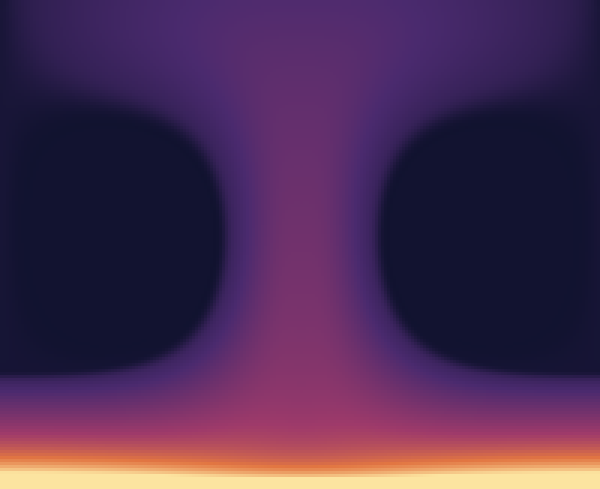
\includegraphics[width=0.40\textwidth]{ehd_q190.png} &
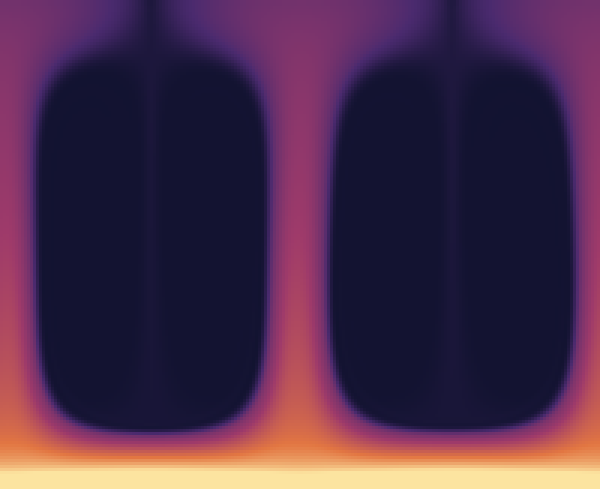
\includegraphics[width=0.40\textwidth]{ehd_q420.png} \\[0.5mm]
\small (a) charge, $T=190$ & \small (b) charge, $T=420$ \\[2mm]
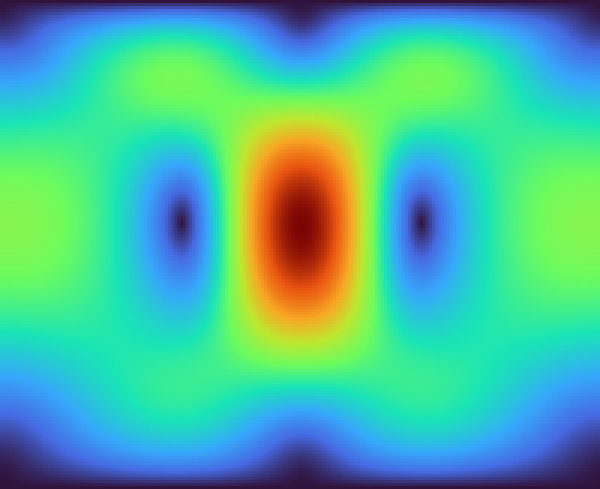
\includegraphics[width=0.40\textwidth]{ehd_u190.png} &
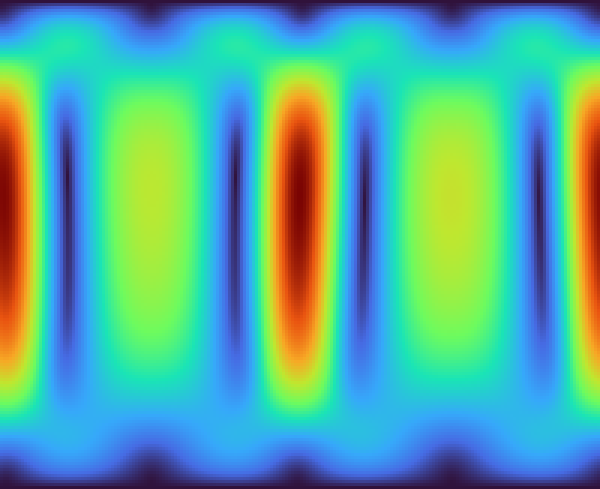
\includegraphics[width=0.40\textwidth]{ehd_u420.png} \\[0.5mm]
\small (c) speed, $T=190$ & \small (d) speed, $T=420$ \\
\end{tabular}
\caption{\textbf{Electroconvection} at $C=10$, $M=10$, $A=0.614$, $n_y=163$,
D2Q9 fluid and charge with D2Q5 potential (\S\ref{sec:ehdconv}). The box is
periodic and twice the reference's width; a free-slip wall is the mirror plane of
a doubled periodic box, so each panel shows \emph{two} of the reference's cells.
Charge is scaled to $[0,0.5\,q_0]$ and saturates: the injector row is $q=q_0$ by
construction, and the dark lobes are the charge-depleted void regions the
reference reads as a hallmark of the subcritical bifurcation. Speed is scaled to
its own peak, $3.76\,u_0$ in (c) and $4.43\,u_0$ in (d); its dark points are the
vortex cores, two in (c) and four in (d). The change of lateral wavenumber
between the columns --- $m=1$ to $m=2$ --- is measured, not imposed, and
reproduces the reference's description of a single cell at $T=190$ becoming a
counter-rotating pair at $T=420$.}
\label{fig:ehdfields}
\end{figure}

\begin{figure}[htbp]
\centering
\begin{tikzpicture}
\begin{axis}[width=7.6cm, height=6.0cm,
  xlabel={$t/t_0$}, ylabel={$u_{\max}/u_0$},
  xmin=0, xmax=42, ymin=0, ymax=5.4,
  grid=both, grid style={line width=.2pt, draw=gray!25},
  major grid style={line width=.3pt, draw=gray!45},
  tick label style={font=\scriptsize}, label style={font=\small},
  legend style={font=\tiny, cells={anchor=west}, draw=gray!50,
                at={(0.98,0.02)}, anchor=south east, fill=white},
  every axis plot/.append style={line width=0.8pt},
  title={\small (a) approach to the steady state}]
  \addplot[opCM]  table[x=t,y=u] {ehd_umax_420_163.dat};
  \addlegendentry{$T=420$, $n_y=163$, D2Q9}
  \addplot[opTRT] table[x=t,y=u] {ehd_umax_420_81.dat};
  \addlegendentry{$T=420$, $n_y=81$, D3Q27}
  \addplot[opMRT] table[x=t,y=u] {ehd_umax_190_163.dat};
  \addlegendentry{$T=190$, $n_y=163$, D2Q9}
  \addplot[opBGK] table[x=t,y=u] {ehd_umax_190_81.dat};
  \addlegendentry{$T=190$, $n_y=81$, D3Q27}
  \addplot[black, dashed, line width=0.6pt, forget plot, domain=0:42, samples=2]
    {4.44};
  \addplot[black, dashed, line width=0.6pt, forget plot, domain=0:42, samples=2]
    {3.70};
\end{axis}
\end{tikzpicture}\hfill
\begin{tikzpicture}
\begin{axis}[width=7.6cm, height=6.0cm,
  xlabel={$y/H$}, ylabel={$q/q_0$},
  xmin=0, xmax=1, ymin=0, ymax=1.03,
  grid=both, grid style={line width=.2pt, draw=gray!25},
  major grid style={line width=.3pt, draw=gray!45},
  tick label style={font=\scriptsize}, label style={font=\small},
  legend style={font=\tiny, cells={anchor=west}, draw=gray!50,
                at={(0.98,0.98)}, anchor=north east, fill=white},
  every axis plot/.append style={line width=0.8pt},
  title={\small (b) hydrostatic profile against Eq.~(78)}]
  \addplot[gray!55, line width=2.2pt] table[x=y,y=qana] {ehd_hydro_C0p1.dat};
  \addlegendentry{analytic}
  \addplot[gray!55, line width=2.2pt, forget plot] table[x=y,y=qana] {ehd_hydro_C1.dat};
  \addplot[gray!55, line width=2.2pt, forget plot] table[x=y,y=qana] {ehd_hydro_C10.dat};
  \addplot[opBGK] table[x=y,y=qnum] {ehd_hydro_C0p1.dat};  \addlegendentry{$C=0.1$}
  \addplot[opMRT] table[x=y,y=qnum] {ehd_hydro_C1.dat};    \addlegendentry{$C=1$}
  \addplot[opCM]  table[x=y,y=qnum] {ehd_hydro_C10.dat};   \addlegendentry{$C=10$}
\end{axis}
\end{tikzpicture}
\caption{\textbf{Electrohydrodynamics.} (a) Peak velocity against time for the
four production runs (\S\ref{sec:ehdconv}); dashed lines are the reference's
converged values, $3.70$ and $4.44$. The $T=420$ pair separates: D3Q27 converges
$4.55\%$ below D2Q9 at $n_y=81$, and refining brings D2Q9 down onto the
published value. All four overshoot near $t/t_0\approx1$ before settling.
(b) Hydrostatic charge profiles at $H=80$ against the analytic solution
(\S\ref{sec:ehdhydro}), thick grey.}
\label{fig:ehdplots}
\end{figure}

\subsubsection{The closed square cavity, and the electric Nusselt number}
\label{sec:ehdcavity}

Their Sec.~3.2.3, after Zhang et al.: a square $A=1$, $L_x\equiv L_y$, with
\emph{every} wall closed,
\begin{equation}
  \uu = \bm 0,\qquad \partial_x q = 0,\qquad \partial_x\varphi = 0
  \qquad\text{at } x = 0,\,L_x .
  \label{eq:cavwalls}
\end{equation}
Three things change from \S\ref{sec:ehdconv}, and each changes what the case can
be trusted to say.

\paragraph{The side walls are real.} \S\ref{sec:ehdconv} has free-slip sides and
is run in a doubled periodic box precisely so that there is no lateral boundary
to discretise. Equation \eqref{eq:cavwalls} is not a mirror --- $\uu=\bm 0$ is
not $\uu\!\cdot\!\nn=0$ --- so that escape is closed and the lateral scalar wall
must be built. It is the wall of \S\ref{sec:scalarspec}, and this case is why
that section exists: measured here with the \emph{fluid frozen}, so that nothing
but the charge/potential pair is in play, the two conditions the solver already
had both fail.

\begin{center}
\begin{tabular}{llll}
\hline
lateral scalar wall & $N=41$ & $N=81$ & \\
\hline
none (periodic, not the paper's problem) & $-0.026\,q_0$ & $-0.022\,q_0$ & reference \\
\code{ScalarAdiabatic} (bounce-back)     & non-finite    & non-finite    & inside $0.05\,t_0$ \\
\code{ScalarOutflow} (open, on-node)     & $-0.083\,q_0$ & $-0.279\,q_0$ & $I_0$ $158\,\%$ wrong \\
\code{ScalarSpecular} (mirror, on-node)  & \multicolumn{2}{l}{reproduces the periodic interior} & \\
\hline
\end{tabular}
\end{center}

The entries are the worst excursion of $q$ outside its bound $[0,q_0]$. Two
things are worth reading off. The open boundary gets \emph{worse} under
refinement, which is the signature of a boundary condition that is wrong rather
than merely inaccurate. And $\omega_q\to2$ is unavoidable here rather than
incidental: $\alpha$ is tied to $T$ (below), so the interesting end of the sweep
is the low-diffusion end.

Every wall in this case is therefore on-node --- \code{RegWall} for momentum,
\code{ScalarMoment} for the plates, \code{ScalarSpecular} for the sides --- so it
is one wall family throughout and not two mixed.

\paragraph{The diffusion number is tied to $T$.} Their Sec.~3.2 quotes
$\alpha=10^{-4}$ and Sec.~3.2.3 additionally fixes $\mathit{Sc}=10^{3}$. Those
are the same statement only at $T=1000$, and the definitions say which is the
rule:
\begin{equation}
  \alpha=\frac{D}{K\Delta\varphi},\quad
  \mathit{Sc}=\frac{\nu}{D},\quad
  \nu=\frac{\varepsilon\Delta\varphi}{KT},\quad
  \varepsilon=M^2K^2
  \ \Longrightarrow\
  \alpha=\frac{M^2}{T\,\mathit{Sc}} .
  \label{eq:alphasc}
\end{equation}
$M=10$, $\mathit{Sc}=10^3$ gives $\alpha=0.1/T$, i.e.\ $10^{-4}$ at $T=1000$
exactly. Their Eq.~(81) writes the diffusive flux with the coefficient
$M^2/(T\,\mathit{Sc})$ rather than with $\alpha$, which settles it: $\mathit{Sc}$
is the invariant across the sweep. So $\alpha$ follows $T$, and $\alpha=10^{-5}$
at $T=10^4$ puts $\omega_q$ at $1.9994$.

\paragraph{The answer is an integral, and its divisor is measured.} Their
Eqs.~(81)--(82),
\begin{equation}
  I_e=\frac{1}{V}\int_V\!\Big[q\,(u_y+KE_y)-\frac{M^2}{T\,\mathit{Sc}}\,
  \partial_y q\Big]\,\mathrm{d}V,
  \qquad N_e=\frac{I_e}{I_0},
  \label{eq:ne}
\end{equation}
with $I_0$ the same integral in the hydrostatic state at the same forcing. Every
run here computes its own $I_0$ by solving the same problem with the Coulomb
force switched off and the seed removed, on the same grid, with the same stencils
and the same walls. That is deliberate: $N_e$ is a ratio, so discretisation error
common to the two states divides out, and what survives is the enhancement due to
motion rather than the sum of that and a grid error. Taking $I_0$ from a formula
would put the grid error into $N_e$ undivided.

The formula is still printed, as a \emph{check} on the numerical $I_0$ rather
than as its source. At $D=0$ the hydrostatic current is uniform, $j=KqE$ with
$\mathrm{d}E/\mathrm{d}y=q/\varepsilon$, so
\begin{equation}
  E(y)^2=E_0^2+\frac{2jy}{K\varepsilon},\qquad E_0=\frac{j}{Kq_0},\qquad
  \int_0^H\!E\,\mathrm{d}y=\Delta\varphi,
  \label{eq:j0}
\end{equation}
and one bisection in $j$ closes it. The strongest evidence that the pair is
consistent is not that agreement, though: it is that below the onset of
convection the code returns $N_e=1.0000\pm0.0000$ with the fluid at rest, to
four figures, because numerator and denominator are then literally the same
computation.

\paragraph{What it measures.} $N=129$, $u_0=5\times10^{-3}$, forty drift times with the
last fifteen averaged, from the reference's own initial condition (zero charge, zero
velocity, so the only seed is round-off). Fig.~8's values are digitised from its
log--log axes by eye and carry roughly $\pm0.05$ on the plateau, so nothing here is
scored against them.

\begin{center}
\begin{tabular}{rrrrrr}
\hline
$T$ & $N_e$ & Fig.~8 & diff & Ma & $\mathrm{Re}_{\rm cell}$ \\
\hline
  150 & 1.0000 & ---  & ---      & 0.000 & 0.0 \\
  250 & 1.0003 & 1.03 & $-2.9$\% & 0.001 & 0.0 \\
  500 & 1.5950 & 1.75 & $-8.9$\% & 0.030 & 0.1 \\
 1000 & 1.6963 & 1.88 & $-9.8$\% & 0.048 & 0.4 \\
 1500 & 1.7505 & 1.93 & $-9.3$\% & 0.054 & 0.7 \\
 3000 & 1.9785 & 2.35 & $-15.8$\% & 0.087 & 2.3 \\
 5000 & 2.5974 & 2.80 & $-7.2$\% & \emph{0.138} & \emph{6.2} \\
10000 & 3.3810 & 3.20 & $+5.7$\% & \emph{0.163} & \emph{14.7} \\
\hline
\end{tabular}
\end{center}

The shape is reproduced: hydrostatic below onset, a steep rise, a shallow plateau, then
renewed growth, with $\kappa=+0.35$ over $1500\to10^4$ against Fig.~8's own points at
$0.27$ and its drawn guide at $0.50$. The level sits $9$--$13\,\%$ low wherever the grid
is trustworthy.

\paragraph{Read the last two rows against the last two columns first.} $T=5000$ and
$T=10^4$ are the only entries that look like agreement, and they are the only two that
break this solver's own rules --- Ma against a $0.087$ guideline, and a cell Reynolds
number where the reference's $H=499$ gives $1.6$ and $4.2$. At $T=5000$, $N_e$ is
$2.8558$ at $N=81$, $2.8017$ at $N=129$ and $2.4903$ at $N=201$
($\mathrm{Re}_{\rm cell}=8.5$, $6.1$, $3.6$); unseeded at $N=201$ it is $2.4366$. So the
coarse grid was \emph{passing through} the published value rather than reproducing it,
which is why the apparent agreement there means nothing. Halving $u_0$ at $N=129$ moves
$2.8017$ to $2.7104$, so compressibility is a $3\,\%$ term and not the explanation.

\paragraph{But that ladder must not be extrapolated, and this document did.} An earlier
version concluded from those three grids that refinement moves \emph{away} from the
reference and that the converged deficit is $\sim\!13\,\%$ low. All three are
under-resolved. \S\ref{sec:cudaehd} has since run the reference's own $500^2$ on a T4 at
$\mathrm{Re}_{\rm cell}=1.5$ --- the first properly resolved point in either
implementation --- and it gives $N_e = 3.1010 \pm 0.4139$, i.e.\ $10.8\,\%$ \emph{high}.
The sequence is not monotonic through to the resolved grid, and three points that never
reach a regime cannot be extrapolated into it. At that grid the reference's $2.80$ lies
\emph{inside} the run's own r.m.s., which makes it consistent with the reference rather
than converged to it: the r.m.s.\ is $13\,\%$ of the mean over three drift times.
What survives is the narrower statement --- when the runs that agree are the only ones
breaking your own Mach and cell-Reynolds rules, distrust the agreement.

\paragraph{The seed chooses a branch, and the usual check cannot see it.} This solver's
standing defence of a seed is that it sets the transient and not the answer, tested by
changing its amplitude and watching the converged value hold. In a \emph{subcritical}
bifurcation that test passes and still misleads:

\begin{center}
\begin{tabular}{lrrrr}
\hline
$T=250$ & amp $10^{-2}$ & amp $10^{-4}$ & amp $0$ & Fig.~8 \\
\hline
$N_e$        & 1.3922 & 1.2400 & 1.0003 & 1.03 \\
$u_{\max}/u_0$ & 2.000 & 1.990  & 0.078  & --- \\
\hline
\end{tabular}
\end{center}

Two decades of seed give the same saturated amplitude --- exactly what seed-independence
looks like --- and no seed at all gives no convection. The seed was not setting the
amplitude, it was deciding which branch the flow reached, and the reference starts from
exactly zero. At $T=500$ the unseeded run is also \emph{steady} (r.m.s.\ $0.0007$ against
$0.107$) and closer to the reference, $1.6583$ against $1.75$: there the seed was
selecting a different and worse attractor rather than merely triggering the instability.
The same bistability is what the reference's own \S3.2.1 hysteresis loop is about.

\paragraph{The fields.} Animations of $q/q_0$ at $N=201$ over eight drift times reproduce
each of Fig.~9's four states and the specific features its text names: at $T=250$ a
smooth diffusive layer with no electroconvective structure; at $T=1000$ a single coherent
plume-like roll rising to the centre with clean separation from the lateral layers; at
$T=5000$ multiple filaments and secondary vortices with sharp gradients along the walls;
and at $T=10^4$ irregular plumes climbing \emph{both} vertical walls with counter-rotating
charge spirals in \emph{both} upper corners around a disordered, charge-depleted core.

\begin{figure}[htbp]
\centering
\begin{tabular}{@{}cccc@{}}
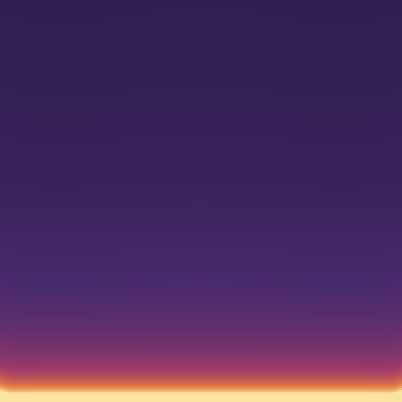
\includegraphics[width=0.235\linewidth]{fig/cav_q_250.png} &
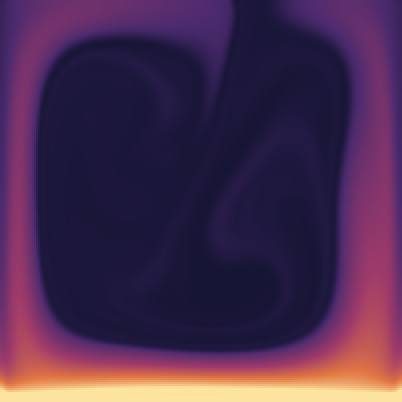
\includegraphics[width=0.235\linewidth]{fig/cav_q_1000.png} &
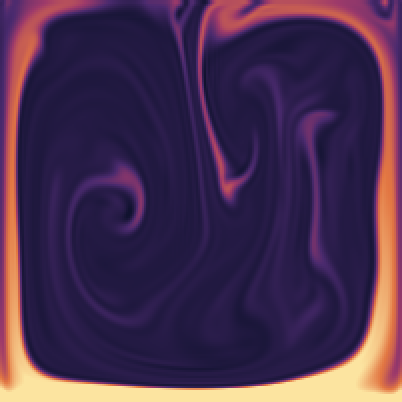
\includegraphics[width=0.235\linewidth]{fig/cav_q_5000.png} &
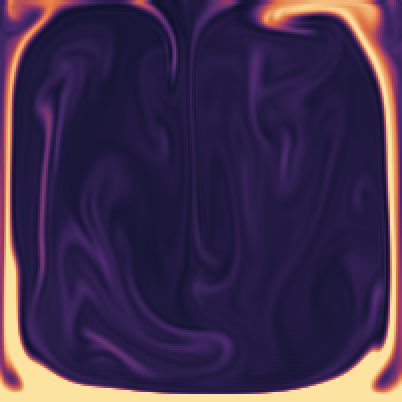
\includegraphics[width=0.235\linewidth]{fig/cav_q_10000.png} \\
\small (a) $T=250$ & \small (b) $T=1000$ & \small (c) $T=5000$ &
\small (d) $T=10^4$ \\
\end{tabular}
\caption{\textbf{Closed square cavity}: charge density $q/q_0$ at $t/t_0=8$,
$201\times201$, injector along the bottom edge (\S\ref{sec:ehdcavity}). Colour is
linear on $[0,\,0.5\,q_0]$ and saturates, as in Fig.~\ref{fig:ehdfields}. These are
the four states of the reference's Fig.~9 and they carry the features its text
names individually: (a) a smooth diffusive layer with no electroconvective
structure, the flow still hydrostatic; (b) a single coherent plume-like roll
rising toward the centre, cleanly separated from the lateral layers; (c) multiple
filaments and secondary vortices, with sharp gradients along the walls; (d)
irregular plumes climbing \emph{both} vertical walls, counter-rotating charge
spirals in \emph{both} upper corners, and a disordered, charge-depleted core.
Panel (a) is run unseeded --- with a seed the cavity convects at $T=250$, which is
the branch selection discussed above --- and (b)--(d) carry a $10^{-4}q_0$
perturbation so the flow is developed inside the window.}
\label{fig:cavfields}
\end{figure}

\paragraph{What it does not do.} It does not run the reference's $500^2$ grid, which is
what $\mathrm{Re}_{\rm cell}$ says $T\ge5000$ actually needs; on this hardware that is
about five hours for a single $T$. The $9$--$13\,\%$ deficit is therefore \emph{measured}
but not \emph{explained} --- resolution and Mach number are both excluded as the whole
cause, and no third candidate has been tested. The charge dips to $-0.028\,q_0$ at
$T=5000$, a small but genuine violation of the maximum principle, and it appears only in
the under-resolved runs.

%==============================================================================
%==============================================================================
\section{Demonstrator: flow in a patient-specific aorta}
\label{sec:aorta}

Everything else in this document runs on a geometry described by a formula. This
one loads a voxel array off disk. It is included as a \emph{demonstrator}, not as
a validation case, and the distinction is worth stating precisely because the
figures are seductive: there is no analytic solution here, no reference data is
compared against, and \textbf{no number in this section is a claim of accuracy}.
What it demonstrates is that the solver runs unmodified on a geometry with no
symmetry and no closed form --- \code{set\_geometry} already takes an arbitrary
predicate, so real geometry needed a reader, not a new solver.

\subsection{Geometry and its verification}
\label{sec:aortageom}

\code{src/io/VoxelGeometry.hpp} reads the flat binary produced by voxelising a
SimVascular surface mesh (case \code{0074\_H\_AO\_H}): $109\times184\times361 =
7\,240\,216$ voxels at a pitch of $0.0616$\,cm, tagged $0$ solid, $1$ fluid,
$2$ inlet, $3$ outlet. Solid is $83.65\%$ of the box; the lumen is $16.31\%$.
The optional second inlet normal is detected by \emph{file size}, not by stream
state --- guessing from the stream would silently read 24 bytes of the tag array
as doubles on a file that does not carry one.

Three checks were run on the geometry before any flow was believed.

\begin{enumerate}[leftmargin=1.4em,itemsep=3pt]
\item \textbf{Connectivity.} A six-connected flood fill seeded from an inlet
  voxel reaches $1\,184\,057$ of $1\,184\,057$ non-solid voxels: one lumen, no
  isolated pockets. This check exists because a single constant-$x$ plane
  through this vessel cuts it into \emph{two} disconnected regions --- the aortic
  root and the arch --- which looks exactly like a hole in the mesh and is not
  one. The projected silhouette is a single connected region, as the flood fill
  requires it to be.

\item \textbf{Caps.} Under six-connectivity the inlet fragments into $303$ pieces
  and the outlets into $270$. This is not damage: an oblique plane on a voxel
  grid is diagonally connected, not face-connected. By centroid they are one
  inlet and four outlets --- three arch branches and the descending aorta.

\item \textbf{Domain edges.} $1283$ fluid voxels sit on the box boundary carrying
  no cap tag. Were the domain periodic these would wrap, connecting the
  descending aorta to the arch and corrupting the field silently. It is not:
  the case constructs \code{Domain(nx,ny,nz,false,false,false)}, and
  independently there are \emph{zero} fluid-to-fluid wrap pairs on any axis. The
  mesh is clipped flush against the box there and those voxels act as wall.
\end{enumerate}

\subsection{Boundary conditions}
\label{sec:aortabc}

\paragraph{The vessel wall} is halfway bounce-back on solid voxels, which under
Esoteric Pull costs nothing: bounce-back is the identity on the storage, so solid
cells are skipped outright --- no load, no store, no arithmetic
(\S\ref{sec:esopull}). The population a fluid node emits toward the wall sits
untouched for one step and is read back reversed on the next, placing the no-slip
surface midway between the last fluid node and the first solid node. Halo cells
are flagged \code{Excluded} and skipped by the same mechanism, so the box faces
behave identically.

\paragraph{The inlet} is a regularised velocity wall along the cap normal stored
in the file. The cap is oblique to the voxel axes, so it has no single face
normal; it is given \code{NrmCorner}, whose unknown set is built geometrically
per node rather than from an axis. Using a face normal instead would drive flow
into the wall.

\paragraph{The outlets} are left at fixed pressure rather than a prescribed flow
split, so the division of flow between the branch vessels is an \emph{output}
rather than an input. Imposing $\uu=0$ there would close the domain --- measured
as mass rising monotonically, $+8.5\e{-3}$ in 2000 steps.

\paragraph{Conserving outflow.} The outlet overwrites its nodes every step, so
whatever density is imposed is injected regardless of what arrived: pinning
$\rho=1$ makes the boundary a mass source and sink, and inlet and outlet fluxes
then differ by ${\sim}60\%$ with no way to tell which is wrong. Closing a loop on
\emph{total mass} instead makes it conserving --- raise the outlet density when
mass is lost, lower it when mass accumulates. The fixed point is the density at
which what leaves equals what enters, and it is found rather than assumed. Two
details are load-bearing. The error must be normalised by total mass, not by
outlet-node count: normalising by the latter gives an error of order $3$, which
saturates the clamp, reverses the flow and diverges the run in 1500 steps. And
the controller is held off until the vessel has filled, since during filling mass
\emph{should} be changing and the loop otherwise fights the physics.

Note that the finite-difference corner-stress path is disabled for this case. It
walks a two-node stencil off each wall node; in a box those neighbours are fluid
or wall, but in a vessel they are frequently \emph{solid}, whose populations
Esoteric Pull never updates, so the stencil reads stale memory and feeds garbage
stress into the inlet. The local closure is used instead until that path is made
geometry-aware.

\subsection{Steady inflow}
\label{sec:aortasteady}

$\mathrm{Re}=50$ on the inlet cap's equivalent diameter $D = 2\sqrt{A/\pi} =
32.9$ lattice units, $U=0.02$, $\nu=1.3167\e{-2}$, $\tau=0.5395$, D3Q27 central
moments. After $13\,500$ steps $|\uu|_{\max}$ is $4.11\e{-2}$, the outlet
density $0.99765$ and the mass error $-3.6\e{-5}$, oscillating about zero ---
which is the conserving outflow working.

These are \emph{not} the numbers this section carried before 2026-09-13, and the
difference is a corrected boundary rather than a retuned case. \code{FluidSolver}
decided which populations at a regularised wall are unknown by testing the source
cell for \code{Excluded} alone, which is right for a wall flush with the domain
edge and blind to one with a \code{Solid} neighbour --- and the inlet and outlet
caps here are exactly that, \code{RegWall} surrounded by solid vessel. The
population arriving from a solid is a bounce-back of the node's own emission and
carries no interior information; it was being treated as known. Every velocity in
this section was therefore about $40\,\%$ too high: $|\uu|_{\max}$ read
$7.2\e{-2}$ and $p_{99.9}$ read $2.6\e{-2}$, against $4.11\e{-2}$ and
$1.50\e{-2}$ now. The defect was found on \code{validation/shercliff.cpp}, which
has an exact solution; nothing in this case could have caught it.

One claim is also weaker than it was. ``Steady'' overstates the state at
$13\,500$ steps: a ${\sim}1500$-step oscillation of the mass servo is still
decaying there, its envelope narrowing from $4.1\e{-4}$ to $2.7\e{-4}$ in mass
over the last few thousand steps, and $|\uu|_{\max}$ still swings a few per cent
between probes. It is converging, not converged.

The inlet flux is $12.98$ in lattice units, and this is worth one sentence
because measuring it is less obvious than it looks. Summing over \emph{every}
exposed face of the cap gives $|\sum \nn_{\rm face}| = 653.2$ pointing within
$0.65^\circ$ of the normal stored in the file, so $U A\cos\theta = 0.02 \times
653.2 \times 0.9935 = 12.98$. Filtering the faces by direction to exclude the
vessel wall was tried and is \emph{wrong} --- it double-weights by the projection
and drove the figure down to $10.38$. The lateral wall faces already cancel in
the vector sum; that is what makes the identity $\sum\nn_{\rm face} = A\nn$ hold.

The outlet flux is \textbf{not} a valid measure for this boundary and is not used
as one: the condition overwrites populations, so a flux summed through it
reports the imposed state rather than what the flow delivered. Mass conservation
is the trustworthy check.

\subsection{Pulsatile inflow}
\label{sec:aortapulse}

The inlet is driven by the waveform used in the source project, reproduced
unchanged so the two are comparable:
\begin{equation}
  \frac{U(t)}{U_0} = \min\!\left(1,\frac{t}{t_{\rm ramp}}\right)
    \Big[0.15 + 0.85\,w(\phi)^{3/2}\Big],
  \qquad
  w(\phi) = \tfrac12 + \tfrac12\sin\!\Big(2\pi\phi - \tfrac{\pi}{2}\Big),
  \label{eq:aortawave}
\end{equation}
with $\phi = (t \bmod T)/T$: a ramp from rest, then a cycle between a diastolic
floor at $15\%$ of peak and a systolic peak, the upstroke sharpened by the $3/2$
power. $\phi=0$ is the diastolic minimum and the systolic peak falls at
$\phi=0.5$. Here $T=2000$, $t_{\rm ramp}=800$, and $U_0$ is the systolic peak.

Since the direction is fixed by the cap normal and only the magnitude varies, the
whole drive is a scale on the deduplicated wall-velocity table
(\code{set\_wall\_velocity\_scale}), not a per-node update, and costs nothing per
step. The scale multiplies a saved copy of the original table rather than the
live one: scaling in place would compound, and a waveform bounded in $[0,1]$
would become a product of its own history and decay to zero within a few hundred
steps --- which would look like a plausible physical relaxation and is not one.

The parameter that characterises a pulsatile flow is not $\mathrm{Re}$ but the
Womersley number, which fixes how far the oscillating shear layer penetrates in a
beat:
\begin{equation}
  \alpha = \frac{D}{2}\sqrt{\frac{2\pi}{T\nu}} = 7.05 ,
  \label{eq:womersley}
\end{equation}
in the physiological range for an aorta. The drive is exact beat after beat:
$Q_{\rm in}$ reaches $-12.98043$ at every systolic peak and $-1.947065$ at every
trough, identical to five digits across six cycles.

\paragraph{Convergence.} The viscous diffusion time across the vessel is
$R^2/\nu = 15\,807$ steps, which is $7.9$ beats. This run is $60\,000$ steps,
$3.8$ diffusion times, and it is converged: sampled at matched phase over the
final three beats, \emph{every} statistic of the speed field repeats to every
digit printed --- $\langle|\uu|\rangle = 2.5007\e{-3}$ and $p_{99.9} =
1.0446\e{-2}$ at the systolic peak for beats $26.5$ through $29.5$ alike.

$\alpha$, $R^2/\nu$ and the beat count all moved on 2026-09-13 and all for one
reason: $D$ was being taken from the cap's VOXEL COUNT, which overstates an
oblique staircase cap by $1/\max|n_i|$ and gave $32.9$ lattice units against a
true $28.8$. $\alpha$ goes as $D$ and $R^2/\nu$ as $D^2$, so the error
propagated into both. The speeds moved separately and for the wall reason given
in \S\ref{sec:aortasteady}.

\begin{center}\small
\begin{tabular}{clcccc}
\hline
$\phi$ & step & mean & median & $p_{99}$ & $|\uu|_{\max}$ \\
\hline
0.0 & 54000 & 0.00364663 & 0.00238384 & 0.0153191 & 0.0565515 \\
0.0 & 56000 & 0.00364663 & 0.00238384 & 0.0153191 & 0.0565515 \\
0.0 & 58000 & 0.00364663 & 0.00238384 & 0.0153191 & 0.0565515 \\
0.5 & 55000 & 0.00483408 & 0.00495437 & 0.0104059 & 0.0320153 \\
0.5 & 57000 & 0.00483408 & 0.00495437 & 0.0104059 & 0.0320153 \\
0.5 & 59000 & 0.00483408 & 0.00495437 & 0.0104059 & 0.0320153 \\
\hline
\end{tabular}
\end{center}

\noindent The residual differences are in the eighth digit, which is round-off.
The outlet density has stopped moving at $0.99699$, so the mass controller has
found its fixed point rather than still walking toward one. An earlier
$12\,800$-step run --- $0.62$ diffusion times --- was reported in a previous
draft of this section as \emph{not} converged, with mean and median still rising
monotonically through six beats. That was accurate, and it is what a run of that
length looks like; it is superseded rather than corrected.

\paragraph{Phase relationships, and a storage effect that is not Womersley.}
Over a converged beat the \emph{mean} speed peaks at $\phi=0.60$ against a drive
peaking at $\phi=0.50$: a lag of $0.10$ of a cycle, $36^\circ$, the expected
sense and order for $\alpha=8$.

The fast tail does the opposite. Both $p_{99}$ and $|\uu|_{\max}$ peak at
$\phi=0$ and reach their \emph{minimum} at systole --- nearly antiphase with the
drive. This is not a transient: it repeats identically across the final three
beats, and it is visible in Fig.~\ref{fig:aortapulse}, where at the diastolic
trough the root has gone pale while the descending aorta carries the fastest
flow in the vessel.

The mechanism is storage, not phase lag. Total mass is not constant over a beat:
it swings by $\pm2.7\e{-3}$, with its minimum at $\phi=0.25$ and its maximum at
$\phi=0.70$, accumulating through systole and discharging through diastole. The
fast tail peaks where that discharge is steepest. A transit-time explanation was
considered and does not survive arithmetic --- at these speeds a fluid particle
needs several beats to cross the vessel.

What this data does \emph{not} settle is where the storage lives. Two candidates
produce the same signature and are not distinguished by the dumps taken here,
which carry velocity but not density: the lattice fluid's own $O(\mathrm{Ma}^2)$
compressibility acting as a compliance chamber, or the fixed-pressure outlet
acting as a reservoir. Either way the effect is numerical rather than
physiological --- the wall is rigid (\S\ref{sec:aorta}, and the Known
Limitations) --- so the antiphase should not be quoted as a Womersley result,
and the fast tail should not be read as a haemodynamic observation.
$|\uu|_{\max}$ in particular is a single staircase-corner voxel and should not
be used at all.

\begin{figure}[htbp]
\centering
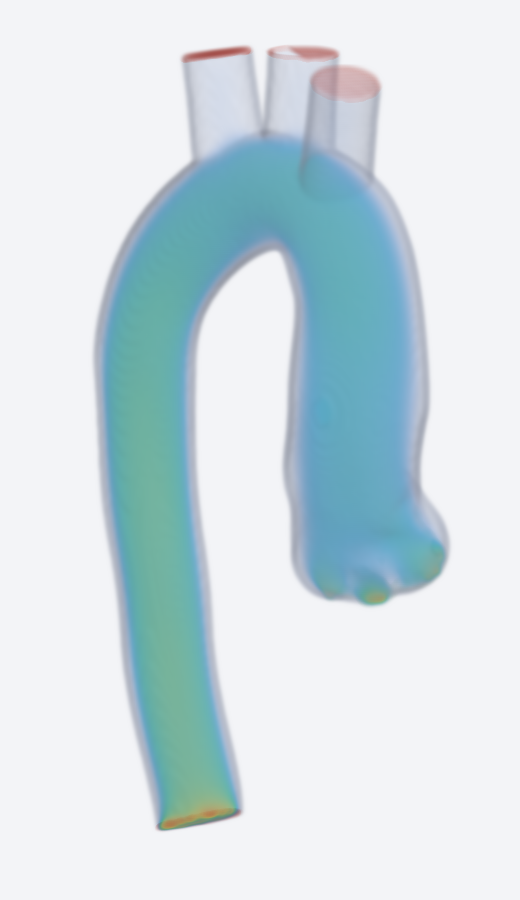
\includegraphics[width=0.32\textwidth]{aorta_steady.png}
\caption{\textbf{Steady inflow at $\mathrm{Re}=50$}, speed, after $13\,500$
steps. Volume rendering: a pale translucent shell wherever the lumen mask has a
gradient, diffuse-shaded off that gradient, with speed-coloured interior showing
through. Inlet cap green at the aortic root, outlet caps red. A single plane
through this vessel cuts it into disconnected islands, which is why the whole
volume is cast rather than sliced.}
\label{fig:aortasteady}
\end{figure}

\begin{figure}[htbp]
\centering
\begin{tabular}{cc}
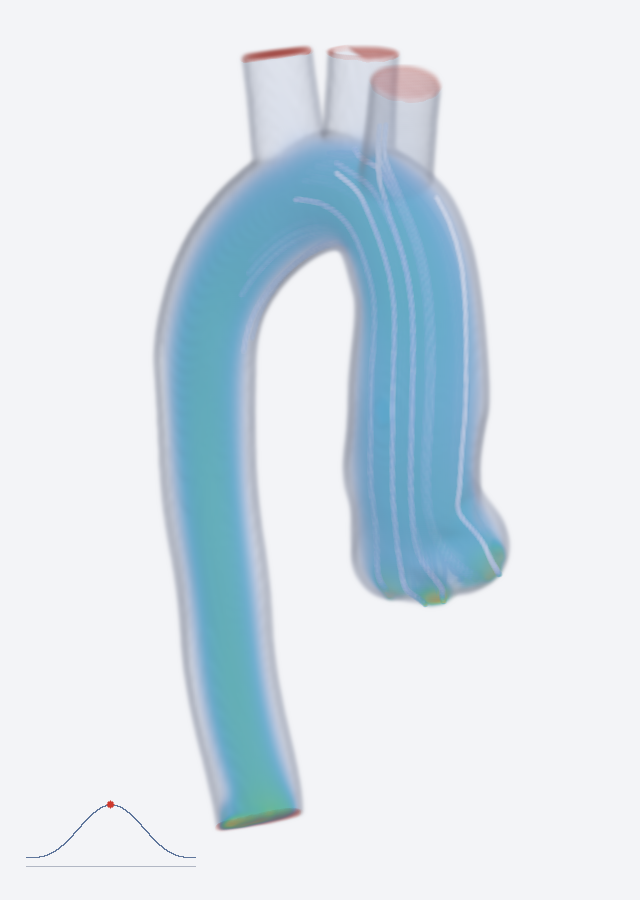
\includegraphics[width=0.32\textwidth]{aorta_systole.png} &
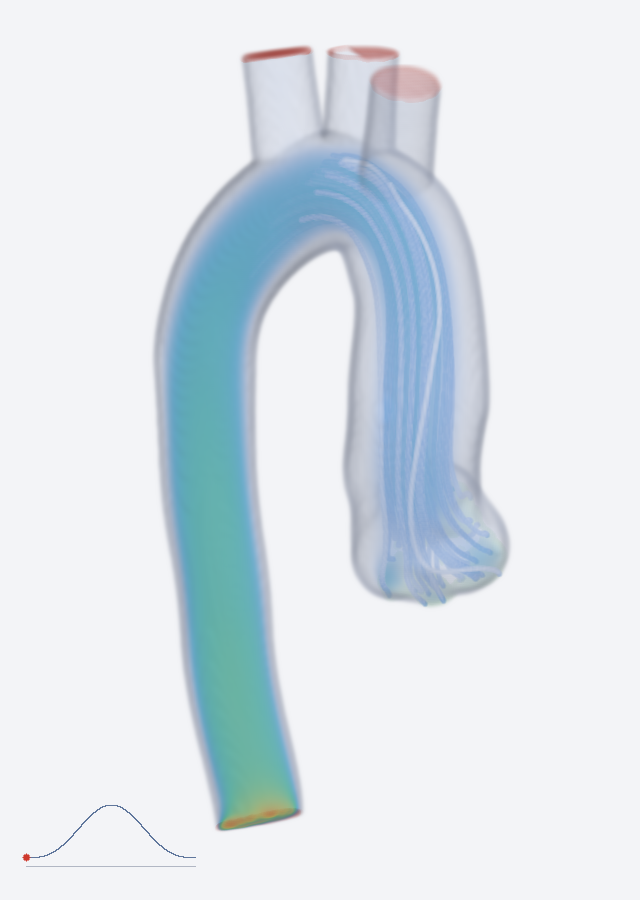
\includegraphics[width=0.32\textwidth]{aorta_diastole.png} \\[1mm]
\small (a) systolic peak, $\phi=0.5$ & \small (b) diastolic trough, $\phi=0$ \\
\end{tabular}
\caption{\textbf{Pulsatile inflow}, converged, $\alpha=7.05$, shared colour
scale, with streamlines traced from the inlet cap through the current field. The
inset traces \eqref{eq:aortawave} with a marker at the current phase. At systole
the root drives a visible jet; at the diastolic trough it has gone pale while the
descending aorta carries the fastest flow in the vessel --- the antiphase fast
tail of \S\ref{sec:aortapulse}, which is a storage-and-release effect and not a
Womersley lag. Both panels are from the same beat, at $3.8$ viscous diffusion
times, where every speed statistic repeats to every printed digit from beat to
beat. The antiphase tail is quantitative, not an impression: at the trough
$p_{99.9} = 1.2317\e{-2}$ and $|\uu|_{\max} = 3.3362\e{-2}$ against
$1.0446\e{-2}$ and $2.0743\e{-2}$ at the systolic peak, so the fastest fluid in
the vessel is genuinely there when the inlet is slowest.}
\label{fig:aortapulse}
\end{figure}

%==============================================================================
\section{Demonstrator: urban pollutant dispersion}
\label{sec:urban}

The second demonstrator, and the second geometry source. A passive scalar is
released into a city and transported by an atmospheric wind over building
geometry read from a height field (\S\ref{sec:heightfield}). Like the aorta,
this is a demonstrator and not a validation case: there is no analytic solution
for a plume in a real city and no measurement to compare against, so nothing
here can fail except by crashing. What \emph{can} be checked is reported as a
number, and one of those numbers turned out to matter.

\subsection{Geometry from a height field}
\label{sec:heightfield}

Urban geometry does not arrive as a voxelised surface mesh. It arrives as
building footprints with heights, so the reader for it is a different one from
the aorta's (\S\ref{sec:aortageom}): a two-dimensional map of building height
in metres, plus a small JSON of grid metadata, with a cell solid when its centre
lies below the local height. That keeps $O(n_x n_y)$ on disk instead of
$O(n_x n_y n_z)$ --- for Manchester, $640$~kB rather than the $9.6$~million
cells it expands to.

Two decisions in that reader are about failure modes rather than features, and
both are there because \emph{none} of the ways it can go wrong produce an
error. A transposed index order rotates the city; a mis-parsed cell size
rescales it; an off-by-one in the solid rule shaves a layer off every roof. All
three run to completion and produce a plausible plume. So a missing key in the
metadata is an error rather than a default --- falling back to a built-in grid
size turns a typo into a silently wrong domain --- and a vertical spacing that
disagrees with the horizontal one is rejected rather than silently stretching
the city. The regression test compares against independently known values
throughout, using a deliberately asymmetric height pattern so that a transpose
changes what is read back.

On the real data the reader is checked against an independent implementation:
Manchester city centre, $400\times400\times60$ at $5$~m, $171\,375$ solid cells
of $9.6$~million ($1.79\%$), tallest column $200.5$~m --- matching cell for
cell.

\subsection{The model, and its principal limitation}

The wind is prescribed: a neutral-stability logarithmic surface layer
$u(z) = (u_*/\kappa)\ln((z+z_0)/z_0)$, horizontal, along a fixed compass
bearing, simply zeroed inside buildings. It has no street-canyon recirculation,
no building wake and no channelling along avenues --- which are precisely the
phenomena an urban dispersion study is about. The scalar side is the validated
one: D3Q7 transport, adiabatic buildings and ground, and the open boundaries of
\S\ref{sec:scalaroutflow}.

The time step follows from capping the fastest cell at a chosen lattice
velocity, and the relaxation rate then follows from the physical diffusivity.
Deriving $\Delta t$ from the wind and $\omega$ from $\Delta t$, rather than
choosing $\tau$ and letting $\Delta t$ fall out, is what keeps the advective
Courant number bounded --- the constraint that actually binds in an
advection-dominated problem.

\paragraph{How not to measure the limitation.} A log profile zeroed inside
buildings is not divergence-free, and it is tempting to look for the damage in a
mass budget. That budget cannot see it. Bounce-back is conservative and
$\sum_i w_i \ci = 0$, so the advective term contributes nothing to
$\sum_i h_i$: the budget closes to round-off however wrong the wind is. The
error appears in the concentration instead, because
$\nabla\!\cdot\!(\uu C) = \uu\!\cdot\!\nabla C + C\,\nabla\!\cdot\!\uu$
and the second term is spurious --- it concentrates the scalar where
$\nabla\!\cdot\!\uu < 0$ and dilutes it where the divergence is positive. So
$\nabla\!\cdot\!\uu$ is the diagnostic, and it is reported separately over
the open cells and over the cells adjacent to a wall, where the zeroing bites
hardest. On Manchester city centre, $400\times400\times60$ at $5$~m:
\[
  \mathrm{RMS}(\nabla\!\cdot\!\uu) = 9.4\times10^{-4}
  \ \text{over}\ 9.06\times10^{6}\ \text{open cells},
  \qquad
  8.4\times10^{-3}\ \text{over}\ 1.14\times10^{5}\ \text{wall-adjacent cells},
\]
a factor of nine worse next to a building. Those two numbers are the
quantitative case for replacing this wind with a solved one, and they are the
reason the original project wrote a Navier--Stokes solver as its second stage.

\subsection{Agreement with the original implementation, and one disagreement}
\label{sec:urbancompare}

The same case run through the original hand-written solver and through this one
agrees exactly where it should. On a synthetic $60\times30\times20$ domain both
give $\Delta t = 0.0129$~s, $\tau = 0.5646$, and identical divergence
statistics --- RMS $1.063\times10^{-3}$ over open cells, $9.213\times10^{-3}$
over wall-adjacent cells, maximum $1.867\times10^{-2}$. Along the plume
centreline the two concentration fields agree to within $0.8\%$ through the
interior. The wind, the scaling, the geometry and the transport are the same
problem.

They part company at the outflow, and it is worth recording which one is wrong.
Steady-state mass here is $11.4\%$ higher than the original's, and the excess
lies entirely near the open faces: $12.5\%$ of this field is within three cells
of one, against $5.9\%$ of the original's. The advective flux through successive
planes settles it:

\begin{center}
\begin{tabular}{rcc}
\toprule
plane $x$ & original & here \\
\midrule
30 & $1.000$ & $1.000$ \\
45 & $0.908$ & $1.052$ \\
55 & $0.840$ & $1.071$ \\
58 & $0.823$ & $1.076$ \\
59 & $0.478$ & $1.076$ \\
\bottomrule
\end{tabular}
\end{center}

\noindent A steady state cannot destroy half its flux at a boundary, and the
original loses from $0.823$ to $0.478$ across a \emph{single} cell. Its exit is
an artificial sink: outgoing populations are discarded and no incoming ones are
supplied, which starves the last cell and pulls material out diffusively for
some distance upstream. The gradual decline from $x=30$ onward is that reach.

The $7.6\%$ rise on this side is not error either, or not all of it. The wind is
sheared, so scalar mixing upward into faster-moving air genuinely increases
$u\,C$ through successive planes while the total flux, advective plus diffusive,
is what is conserved. The condition itself was measured in \S\ref{sec:plume}
against a case with no shear and an analytic answer, where it holds the flux to
$0.038\%$ to the last interior cell.

\subsection{A stability limit that does not announce itself}
\label{sec:urbanstab}

The first attempt at the full city ran to completion, reported no error, and
wrote four hundred megabytes of nonsense. Mass in the domain grew from
$5.6\times10^{1}$ at $t=60$~s to $1.2\times10^{8}$ at $t=90$~s and thereafter by
roughly nine orders of magnitude per frame, reaching $10^{70}$ --- without ever
producing a NaN, which is why the finiteness check in the output loop passed
every time.

The mechanism is the spurious term of the previous section read in the other
direction. Since
$\partial_t C \supset -C\,\nabla\!\cdot\!\uu$, the scalar \emph{grows}
exponentially wherever the divergence is negative, at rate
$|\nabla\!\cdot\!\uu|$. What opposes it is diffusion, which damps a
cell-scale blob at approximately $D_{\rm lat}\pi^2$. Writing the lattice
diffusivity out,
\begin{equation}
  D_{\rm lat} = \frac{D\,\Delta t}{\Delta x^2}
              = \frac{D\,u_{\rm lat}^{\max}}{u_{\rm peak}\,\Delta x},
  \label{eq:dlat}
\end{equation}
which contains no $\Delta t$: \textbf{shortening the time step buys no margin
at all}, because $\Delta t$ cancels between the diffusivity and the velocity
scaling. Only a larger diffusivity, a slower wind or a finer grid helps.

\begin{center}
\begin{tabular}{lcccccl}
\toprule
case & $D_{\rm lat}\pi^2$ &
$\max|\nabla\!\cdot\!\uu|$ & margin &
$\mathrm{rms}\,|\nabla\!\cdot\!\uu|$ & margin & outcome \\
\midrule
synthetic              & $0.159$ & $1.87\!\times\!10^{-2}$ & $8.5\times$ & $1.06\!\times\!10^{-3}$ & $150\times$ & stable \\
Manchester, E, $D=5$   & $0.041$ & $2.32\!\times\!10^{-2}$ & $1.8\times$ & $9.42\!\times\!10^{-4}$ & $44\times$  & diverged \\
Manchester, E, $D=20$  & $0.166$ & $2.32\!\times\!10^{-2}$ & $7.2\times$ & $9.42\!\times\!10^{-4}$ & $176\times$ & stable \\
Manchester, NE, $D=20$ & $0.166$ & $3.28\!\times\!10^{-2}$ & $5.1\times$ & $9.21\!\times\!10^{-4}$ & $180\times$ & stable \\
Manhattan, $D=20$      & $0.152$ & $3.35\!\times\!10^{-2}$ & $4.6\times$ & $2.43\!\times\!10^{-3}$ & $63\times$  & \textbf{exponentiated} \\
Manhattan, $D=35$      & $0.267$ & $3.35\!\times\!10^{-2}$ & $8.0\times$ & $2.43\!\times\!10^{-3}$ & $110\times$ & stable \\
\bottomrule
\end{tabular}
\end{center}

\noindent \textbf{The maximum is the wrong statistic}, and it took a second city
to see it. Read the max-based column on its own: the failures sit at $1.8\times$
and $4.6\times$, the successes at $5.1\times$, $7.2\times$, $8.0\times$ and
$8.5\times$. There is no threshold to draw --- $4.6$ diverges and $5.1$ does not,
eleven per cent apart, and those two runs have the same peak divergence to within
two per cent. Read the rms-based column instead and the failures are at
$44\times$ and $63\times$, the successes at $110\times$, $150\times$, $176\times$
and $180\times$, with a clear gap between. That is where the threshold now sits,
at $100\times$.

The reason is not hard to see once the numbers force the question. The spurious
source is damped at the cell scale by $D_{\rm lat}\pi^2$, so an isolated bad cell
is held down by diffusion from its neighbours; what outruns diffusion is an
\emph{extended} region of divergence. How much of the domain is in that state is
exactly what the rms measures and the max does not. The decomposition is exact,
\begin{equation}
  \mathrm{rms}_{\rm open}|\nabla\!\cdot\!\uu|
  = \sqrt{N_{\rm wall}/N_{\rm open}}\;\,
    \mathrm{rms}_{\rm wall}|\nabla\!\cdot\!\uu|,
\end{equation}
$0.112\times8.22\times10^{-3}$ for Manchester and $0.183\times1.33\times10^{-2}$
for Manhattan, both reproducing the table to three figures --- so the quantity
really is \emph{how much city}, not \emph{how bad is the worst cell}. Manhattan
has $4.3$ times as many wall-adjacent cells as Manchester, $485\,982$ against
$113\,863$, from $50.4\%$ of columns built against $29.9\%$, $6.87\%$ of the
domain solid against $1.79\%$, and buildings to $472$~m against $200$~m.
\textbf{The margin is a property of the geometry}, so a diffusivity calibrated on
one city does not transfer to another, and the code now says so at setup rather
than after fourteen minutes.

Two caveats on the threshold. It is calibrated on \emph{one} failure that was
diagnosed properly --- Manhattan at $63\times$ --- so it is a warning, not a
proof, and both margins are printed because the max is still worth seeing. And
the rms is taken over open cells, so a domain carrying a great deal of empty air
above the rooflines dilutes it; the decomposition above is how to check whether
that has happened.

Neither is $u^{\max}_{\rm lat}$ a lever, which is worth stating because it looks
like one. It scales $D_{\rm lat}$ through Eq.~\eqref{eq:dlat} and it scales
$\nabla\!\cdot\!\uu$ in lattice units by exactly the same factor, so it cancels
out of the ratio entirely.

\subsubsection*{The undershoot is the early warning; the mass test is not}

Mass in the domain cannot exceed what has been injected by any meaningful
factor, and that --- not finiteness --- is what catches a run that has already
failed. It is a poor \emph{early} warning. The Manhattan run at $4.6\times$ never
came close to tripping it: mass tracked injection to within a per cent for
every one of the nine frames it was allowed to write.

What did move, from the first frame, was the undershoot. A first-order
equilibrium with no limiter produces small negative concentrations at sharp
gradients; those are bounded and do not grow, and a few parts in ten thousand of
the peak are expected. An exponentiating $C\,\nabla\!\cdot\!\uu$ is not bounded,
and it appears here first by a wide margin:

\begin{center}
\begin{tabular}{lccc}
\toprule
$t$ (s) & peak $C$ & $\min C$ & $|\min C|/\mathrm{peak}$ \\
\midrule
 18 & $6.40\times10^{-2}$ & $-2.23\times10^{-5}$ & $0.03\%$ \\
 54 & $8.63\times10^{-2}$ & $-2.81\times10^{-5}$ & $0.03\%$ \\
 90 & $1.07\times10^{-1}$ & $-4.74\times10^{-4}$ & $0.44\%$ \\
126 & $1.15\times10^{-1}$ & $-3.57\times10^{-3}$ & $3.09\%$ \\
162 & $1.24\times10^{-1}$ & $-1.31\times10^{-2}$ & $10.53\%$ \\
\bottomrule
\end{tabular}
\end{center}

\noindent A factor of two every eighteen seconds, with the count of cells below
$-10^{-4}$ growing from $53$ to $1137$ over the same span and centred at
$z\approx150$--$190$~m, where the tower tops make the divergence largest. The
run is therefore stopped on the undershoot exceeding half the peak, and warns at
one twentieth of it. At $D=35$ the same diagnostic reads $-9.5\times10^{-9}$ at
$t=108$~s against $-1.5\times10^{-3}$ at $D=20$: five orders of magnitude, and
flat rather than growing.

This is worth stating plainly as a limitation of the prescribed wind rather than
a tuning inconvenience. A larger $D$ is defensible ---
it is a calibrated stand-in for unresolved mixing, not a measured constant, and
$20\,\mathrm{m^2s^{-1}}$ at $5$~m resolution in a city is not extravagant ---
but the reason it is \emph{needed} is that the wind is not divergence-free. A
solved wind removes the spurious source altogether, and with it this constraint.

\subsection{Thirteen per cent that was never missing}
\label{sec:wallslots}

The Manhattan run reported $87\%$ of the release still in the domain and held
there, with the plume nowhere near a boundary. Summing the written field
directly confirms it: the mass within three cells of any face is zero to twenty
decimal places. A steady $13\%$ sink, in the interior, in a scheme whose
collision conserves $\sum_i h_i$ exactly at every node --- $\sum_i w_i = 1$ and
$\sum_i w_i \ci = \bm{0}$, so $\sum_i h_i^{\rm eq} = C$ whatever $\uu$ is --- and
whose streaming is a permutation.

Three controls localised it correctly and could not explain it. The synthetic
case with no wind retained $99.0\%$; a flat height field with the wind on, where
$\nabla\!\cdot\!\uu$ is $0.000$ to machine precision because $\uu=(u(z),0,0)$,
retained $98.6\%$; Manhattan with the same wind retained $87.2\%$. The
difference is the buildings, not the divergence. But every one of those numbers
was produced by the same estimator, and none of them could say whether material
was being destroyed or merely hidden.

A closed box can. \texttt{validation/scalar\_mass.cpp} puts a source inside a
domain whose every face is insulating, so what went in is what must be there,
and adds one feature at a time:

\begin{center}
\begin{tabular}{lrrrr}
\toprule
case & injected & in fluid & error & every slot \\
\midrule
closed box            & $400.000000$ & $397.155123$ & $-0.711\%$ & $400.000000$ \\
$+$ interior block    & $400.000000$ & $390.406451$ & $-2.398\%$ & $400.000000$ \\
$+$ advection         & $400.000000$ & $372.499608$ & $-6.875\%$ & $400.000000$ \\
$+$ wind zeroed in solids & $400.000000$ & $372.499608$ & $-6.875\%$ & $400.000000$ \\
\bottomrule
\end{tabular}
\end{center}

\noindent \textbf{Nothing is lost.} The last column is the injection to
round-off in every case. What is short is the sum of the \emph{macroscopic
field} over fluid nodes, which is what the demonstrator was reporting. Under
Esoteric Pull a population emitted toward a wall spends one step in a slot the
\emph{wall} node owns, and \texttt{compute\_field} sets the field to zero at an
adiabatic node by definition, so that material belongs to no node's field while
it is in flight. Measuring the same sum one step later shows the shortfall is
steady rather than alternating with the parity, so it is a standing boundary
layer: it scales with wall area ($0.7\%$ for a bare box, $2.4\%$ once there is a
block in it) and with the advective flux into walls ($6.9\%$). Over Manhattan's
$6.87\%$ solid fraction it is $13\%$. Manchester's $1.79\%$ is why this never
surfaced before.

Two details are worth keeping. First, the third and fourth rows agree to the
last digit. Zeroing the wind inside solids --- the thing that makes the
prescribed field divergent in the first place --- changes the budget by exactly
nothing, because solid cells are never read and the velocity stored there is
never used. That confirms the claim of \S\ref{sec:urbancompare} that no mass
budget can see the divergence; what that claim did not say is that the
fluid-only sum carries a wall-area bias of its own. Second,
\texttt{scalar\_walls.cpp} covers Dirichlet walls, where mass is deliberately
not conserved --- that is what a fixed-value boundary is for. Nothing covered
the insulating one, which is precisely the boundary that does nothing at all,
and ``costs nothing'' turned out to be a strong claim to leave untested.

The budget now uses \texttt{ScalarSolver::total\_population}, which sums every
slot in the lattice, and reports the fluid fraction beside it rather than in
place of it. With that change the demonstrator reports $100.0\%$ retained and
$\mathrm{d}M/\mathrm{d}t$ of exactly $1.000$ until material actually reaches an
outlet, which is what the column always claimed to mean.

\subsection{The city}

Manchester city centre, $400\times400\times60$ cells at $5$~m --- $2$~km square
and $300$~m deep, $6058$ buildings --- with a $5\,\mathrm{m\,s^{-1}}$ westerly
at $10$~m, $z_0 = 1$~m, $D = 20\,\mathrm{m^2s^{-1}}$ and a continuous release of
one unit per second. The source cell falls inside a building and is lifted clear
of it, so the release is from a roof at $32.5$~m rather than from the street.
Five minutes of physical time is $14\,280$ steps and runs in $801$~s on four
threads of an M1, or $171$~MLUPS.

The plume approaches steady state monotonically: $\mathrm{d}M/\mathrm{d}t$ falls
from $0.97$ to $2.0\times10^{-3}$ over the run while the mass in the domain
plateaus at $1.409\times10^{2}$. It has not fully arrived --- the derivative is
three orders down but not zero --- which is honest for a five-minute release into
a two-kilometre domain at $5\,\mathrm{m\,s^{-1}}$: the leading edge has crossed
roughly $1.5$~km.

\begin{figure}[htbp]
\centering
\includegraphics[width=0.82\textwidth]{fig/urban_mcr_plume.png}
\caption{Urban plume over Manchester city centre after five minutes of
continuous release from a rooftop at $32.5$~m. \emph{Top}: plan view, building
footprints in grey, column-integrated concentration on a logarithmic scale; the
bar is $500$~m. \emph{Bottom}: vertical section along the plume centreline,
vertical scale exaggerated three times, showing the release lifting as it enters
faster-moving air aloft. The wind is a $5\,\mathrm{m\,s^{-1}}$ westerly, so the
plume runs east. Note what the figure does \emph{not} show: the wind is
prescribed, so there is no recirculation behind any of these buildings and no
channelling along the streets the plan view makes so visible.}
\label{fig:urbanplume}
\end{figure}

\paragraph{A second configuration, and what the first one hid.} Releasing at the
centre of the domain into a due-east wind gives only $1$~km of fetch, and the
plume reaches steady state at $t=5$~min --- three fifths of that run is static.
Moving the source to an open pocket in the south-west at $(140,135)$~m and
turning the wind onto the diagonal, toward the north-east, gives $2.6$~km of
fetch; steady state then arrives at $10.8$~min and the plume develops throughout.
The source also sits at street level, $7.5$~m, rather than being lifted onto a
roof as the central cell was.

That change exposed a defect the first configuration could not. The count of
cells used to normalise the release and the set of cells actually injected into
were separate predicates, and they disagreed at $z=0$: the count required
$z>0$ while the injection covers every bulk cell, which since
\S\ref{sec:urban} includes the ground layer. A box centred at $z=1$ therefore
had its per-cell rate computed for three layers and applied to four --- $33\%$
over-injection, visible within eighteen seconds as more scalar in the domain
than had been released, and invisible for any source clearing $z=2$. The two are
now one named predicate, asked twice.

The diagonal wind appears to cost stability margin: zeroing both horizontal
components inside buildings raises $\max|\nabla\!\cdot\!\uu|$ from
$2.3\times10^{-2}$ to $3.3\times10^{-2}$, and the max-based margin of
\S\ref{sec:urbanstab} falls from $7.2$ to $5.1$. That was described here as
``comfortably clear of the $1.8$ that diverged'', on the strength of a mass
budget that stayed sensible for the whole run --- which, as \S\ref{sec:urbanstab}
now records, is not a judgement a mass budget can make.

The configuration was therefore repeated and its undershoot examined. It is
stable, and not marginally so: $\min C$ is bit-identical at $-1.11\times10^{-7}$
for six consecutive frames from $t=45$ to $t=120$~s, while a Manhattan run at
nominally the same margin had grown its undershoot twentyfold over the same span.
What the max-based number was hiding is that the diagonal wind barely changes the
rms at all --- $9.42\times10^{-4}$ to $9.21\times10^{-4}$, a $2\%$ \emph{fall} ---
because it redistributes divergence among the same wall-adjacent cells rather
than adding any. On the statistic that predicts the outcome this is the safest
configuration in the table, at $180\times$.

\paragraph{Negative concentrations.} The scheme undershoots. A first-order
equilibrium with no limiter produces small negative concentrations at sharp
gradients: $3.2$~million cells of $9.6$~million hold values between $0$ and
$-7.9\times10^{-5}$, against a section peak of $5.4\times10^{-2}$ --- a few
parts in ten thousand. They are bounded and do not grow, and \texttt{min C} is
now reported every frame so that they are visible rather than assumed away. The
practical consequence is for anything downstream that takes a logarithm or
treats a negative value as a flag: the plan-view renderer for
Figure~\ref{fig:urbanplume} initially tested \texttt{v < 0} for the building
mask, which is how it came to paint three million undershooting cells as
buildings and hide most of the city.

\subsection{A second city}
\label{sec:urbannyc}

Midtown Manhattan, $400\times400\times100$ cells at $5$~m --- the same $2$~km
square, $500$~m deep, $10\,210$ buildings --- with the same
$5\,\mathrm{m\,s^{-1}}$ wind at $10$~m and $z_0=1$~m, and the same continuous
release of one unit per second from street level at $7.5$~m. Everything that
could be held fixed against \S\ref{sec:urban} was. What could not is the
diffusivity: $D=35\,\mathrm{m^2s^{-1}}$ against Manchester's $20$, for the
reason \S\ref{sec:urbanstab} sets out. Fifteen minutes of physical time is
$46\,665$ steps and $51$ frames.

\begin{figure}[htbp]
\centering
\includegraphics[width=\textwidth]{fig/urban_nyc_collage.png}
\caption{Midtown Manhattan at steady state, fifteen minutes into a continuous
street-level release. Three shells of concentration, at the levels enclosing
$95\%$, $80\%$ and $50\%$ of the plume's mass --- chosen from this frame rather
than carried over from another run, since the same release spread over $2$~km
carries an order of magnitude less than it does over $200$~m. \emph{Left}: the
skyline broadside to the plume, which runs left to right along the avenues.
\emph{Top right}: the same view from street level, showing the release
threading between the towers. \emph{Bottom right}: plan view, with the
Commissioners' grid visible; the wind bearing was measured out of the height
field, not looked up. Every figure in the caption strip is read from the run's
own log, and the plan-view line is measured from this frame. The animation is
\texttt{doc/fig/manhattan\_dispersion.mp4}.}
\label{fig:urbannyc}
\end{figure}

\paragraph{The wind direction was measured, not assumed.} Manhattan's street
grid is not aligned with north, and rather than look the angle up it was
recovered from the height field: rays marched from every open column, in every
direction, recording how far they travel before meeting a building. The mean
free run peaks at two orthogonal bearings, $28^\circ$ and $118^\circ$ --- $385$~m
along the second, $285$~m along the first --- which is the Commissioners' Plan of
1811, extracted from a $400\times400$ array of heights with no knowledge of what
city it is. The wind was then aimed along $28^\circ$, up the avenues, giving
$2.10$~km of fetch from a source in an open pocket in the south of the domain.

\paragraph{Steady state, and a budget that now says what it means.} The plume
reaches steady state at about $11.4$~min, where $\mathrm{d}M/\mathrm{d}t$ falls
below $2\%$ of the injection rate; by the last frame it is $1.8\times10^{-3}$ and
the mass in the domain has plateaued at $3.670\times10^{2}$ against
$8.817\times10^{2}$ injected. That $41.6\%$ retained is a real statement about
where the release has gone --- the remaining $58\%$ has left through the outlets
--- which it was not before \S\ref{sec:wallslots}: the same run reported under the
old fluid-only sum would have shown $87\%$ and held there while the plume was
still in the middle of the domain. The companion column reads $92.0\%$ for the
whole run, unchanging: that is the fraction the plotted field sees, and the $8\%$
gap is Manhattan's wall area.

The undershoot is $-8.08\times10^{-9}$ and does not move for any of the $51$
frames --- the total negative mass is $3\times10^{-7}$, or $0.00\%$ of the plume.
At $D=20$ the same configuration reached $-1.3\times10^{-2}$ by $t=162$~s and was
doubling every eighteen seconds.

\paragraph{The canyons hold the plume, but only near the source.} The plan view
of a city plume invites a claim about street channelling, and the caption on the
Manchester animation made one: \emph{isotropic lateral spread --- the streets do
not steer it}. On a regular grid of canyons with the wind aimed along one of its
axes that is worth measuring rather than asserting, so
\texttt{doc/fig/plume\_stats.py} bins the last frame by downwind distance along
the plume's own axis and compares the concentration-weighted crosswind spread
below and above the rooflines:

\begin{center}
\begin{tabular}{rccccc}
\toprule
$s$ (m) & $\sigma_n$ street & $\sigma_n$ aloft & ratio &
$\langle z\rangle$ street & street fraction \\
\midrule
 131 & $39.5$  & $53.8$  & $0.73$ & $26.2$ & $75.5\%$ \\
 394 & $57.7$  & $72.1$  & $0.80$ & $31.5$ & $47.8\%$ \\
 656 & $78.1$  & $80.6$  & $0.97$ & $31.9$ & $33.8\%$ \\
 919 & $99.3$  & $94.9$  & $1.05$ & $32.1$ & $32.4\%$ \\
1181 & $99.8$  & $99.9$  & $1.00$ & $33.2$ & $25.7\%$ \\
1706 & $120.0$ & $123.0$ & $0.98$ & $31.3$ & $22.7\%$ \\
1969 & $130.3$ & $120.4$ & $1.08$ & $33.0$ & $19.7\%$ \\
\bottomrule
\end{tabular}
\end{center}

\noindent Within the first $130$~m the plume is $27\%$ narrower below the
rooflines than above them, and by $650$~m the two are the same. The last column
says why: the fraction of the plume still below roof level falls from $76\%$ to
$20\%$, so there is progressively less left for the canyons to hold. The
street-level material that remains does not rise --- its mean height sits at
$32$~m the whole way --- while the part aloft climbs from $91$~m to $164$~m as it
mixes into faster air.

That is a confinement effect and \emph{not} a channelling one, and the
distinction matters here more than it would in a solved wind. The prescribed
field blows in a straight line by construction: nothing in this model can steer
a plume along a street. What the buildings do is block, and being opaque to the
scalar is on its own enough to produce the near-field narrowing. A solved wind
would add the channelling this one cannot represent, and the honest reading of
the table is as a lower bound on how much the geometry matters.

The caption on the animation is generated from exactly this measurement rather
than written by hand, for the reason the Manchester caption illustrates: pointed
at a second city, a caption made of literals states the first city's name, cell
count and fetch with complete confidence.

\subsection{Solving the wind}
\label{sec:urbansolved}

The wind can instead be solved: D3Q27 TRT Navier--Stokes on the same geometry,
sharing the Domain, $\Delta x$ and $\Delta t$ with the scalar, so the fluid's
lattice velocity \emph{is} the scalar's and the two couple with no conversion.
TRT rather than BGK because the effective viscosity puts $\tau^+$ within a few
thousandths of $1/2$, where BGK is unusable and TRT's free antisymmetric rate is
exactly the lever required; $\Lambda = 3/16$ additionally places the
bounce-back wall halfway, so a voxelised building is the size it looks. Starting
from the undisturbed profile rather than from rest leaves only the wakes to
develop, and the solve converges to a relative change of $2\times10^{-7}$ in
$7000$ steps.

\begin{figure}[htbp]
\centering
\includegraphics[width=0.78\textwidth]{fig/urban_wind_compare.png}
\caption{Vertical section through a building, wind speed, both panels on the
same scale. \emph{Top}: the prescribed logarithmic profile --- flat horizontal
layers, unaware that the building is there. \emph{Bottom}: the solved field ---
upstream stagnation, acceleration over the roof, and a slow wake in the lee
recovering over roughly twenty cells. Along the centreline at mid-building
height the prescribed field is $4.34\,\mathrm{m\,s^{-1}}$ everywhere, while
the solved one falls to $1.37$ approaching the building and $0.30$ behind it.
The bright stripe at the right edge is the outlet-corner artefact discussed
below, left visible rather than cropped. The colour scale is the $98$th
percentile, not the maximum: that artefact reaches $29\,\mathrm{m\,s^{-1}}$ and
scaling to it renders every physical feature in the bottom quarter of the ramp
--- the same trap as the aorta volume render, where $p_{100}$ was $2.7$ times
$p_{99.9}$.}
\label{fig:urbanwind}
\end{figure}

\paragraph{The interior is right, and is the point.} \emph{All the figures in
this and the next paragraph are the synthetic $60\times30\times20$ case}, which
for a long time was the only geometry this mode had ever been run on; the city
results are in \S\ref{sec:urbansolvedcity}. Three cells clear of every
face, the divergence falls from $\mathrm{RMS} = 1.27\times10^{-3}$ prescribed to
$2.12\times10^{-4}$ solved --- a factor of six --- and the peak speed is
$8.80\,\mathrm{m\,s^{-1}}$ against a $7.74\,\mathrm{m\,s^{-1}}$ free stream, a
$14\%$ speed-up over the building. That is a result the prescribed profile
cannot produce at all, and the divergence drop is the spurious source of
\S\ref{sec:urbanstab} shrinking, which is what drove both the concentration
error and the stability floor.

\paragraph{The domain edges are not right.} Where the pressure outlet meets the
velocity-prescribed lateral and top faces the corner is over-determined, and a
jet forms along it: $31.6\,\mathrm{m\,s^{-1}}$ and
$\nabla\!\cdot\!\uu = 9.5\times10^{-2}$, against $8.8$ and $7.0\times10^{-3}$
in the interior. This is why the global maxima look worse than the prescribed
field's while every interior statistic is better, and it is the reason the
diagnostics now report interior-only figures and say whether the worst
divergence sits on a domain face --- without which the two were not separable.

Two remedies were tried. Giving the edges the free-stream profile removed the
sixty-eight inert outflow nodes, whose donor lay on an adjoining wall, but did
\emph{not} remove the jet, which locates the cause in the mixed condition
itself rather than in the donor lookup. The identified fix is periodic lateral
boundaries, the standard atmospheric arrangement, which deletes two of the four
offending faces outright.

\subsection{The same mode on a city, and the two things that stopped it}
\label{sec:urbansolvedcity}

Everything above is the synthetic case. Pointed at Manchester the mode produced
a NaN within $500$ steps --- in FP64 as well as FP32, so not a precision effect
--- and it did so at the $\tau^+$ the synthetic case had converged at. Bisecting
by geometry:

\begin{center}\small
\begin{tabular}{lccll}
\toprule
case & buildings & on faces & outcome & peak / free stream \\
\midrule
synthetic $60\times30\times20$   & 1    & no  & converges, $5.7\times10^{-7}$    & $4.1\times$ \\
flat $200\times200\times150$     & none & --- & no NaN, residual $6.5\times10^{-2}$ & $4.4\times$ \\
Manchester $400\times400\times60$ & 6058 & \textbf{yes} & \textbf{NaN by step 500} & --- \\
Manchester, 8-cell clear margin  & 2083 & no  & no NaN, residual $2.7\times10^{-1}$ & $2.6\times$ \\
\bottomrule
\end{tabular}
\end{center}

\paragraph{A face cell shadowed by a building is ill-posed.} The regularised
condition reconstructs the density at a wall node from the populations that
streamed into it, split by the wall normal into known and unknown, and that
split assumes the known ones arrived from the interior. When the cell one step
inward is a building, what actually arrives is bounce-back off that building,
the reconstructed density is not a density, and the solve diverges. Manchester
has $3975$ built columns touching the domain edge; clearing an eight-cell band
removes the NaN outright, which is what identified the cause. Only $141$ cells
are \emph{actually} shadowed --- a face cell with solid immediately inward ---
and those $141$ were enough to destroy a nine-million-cell solve. They are now
closed as \texttt{Solid}, which extends the building by the one cell it was
already effectively occupying and turns an ill-posed node into a well-posed
wall. That also subsumes the ``outflow node has no fluid neighbour and is
inert'' case: the same geometry seen from the outlet side, previously left
frozen rather than closed.

\paragraph{Periodic laterals, and what they cost.} \texttt{-lateral periodic}
makes the $y$ faces periodic, deleting two of the four junctions where a
velocity-prescribed wall meets a pressure outlet. Periodicity is handled inside
\texttt{Domain::fill\_neighbours}, so neither solver needed changing; the
divergence diagnostics did, because $y=0$ and $y=n_y-1$ become ordinary
interior cells whose neighbours wrap, and omitting them would drop $0.5\%$ of
the domain from an rms the stability threshold is built on.

The two fixes are independent, and it is worth being explicit that periodic
laterals alone do \textbf{not} cure the NaN --- they leave the inlet and outlet
faces, where the same shadowing occurs. Both are required.

What periodicity costs is a modelling choice rather than accuracy, and the run
now states it rather than leaving it implicit: the domain becomes an infinite
strip, the city repeats every $2$~km across the wind, and a plume drifting
sideways out of one edge re-enters at the other. The seam is not smooth either,
since real building heights at $y=0$ and $y=n_y-1$ were never chosen to match:
$220$ of Manchester's $400$ edge columns disagree, worst by $48$~m. That count
is printed, and a separate warning fires if the wind has a cross-wind component,
because the plume is then advected through the seam rather than merely diffusing
across it.

\paragraph{A solved wind inverts which statistic misleads.} With both fixes,
Manchester at $8000$ flow steps --- one flow-through time at
$u^{\max}_{\rm lat} = 0.05$, so a developing field and not a converged one:

\begin{center}\small
\begin{tabular}{lccc}
\toprule
 & prescribed & solved & change \\
\midrule
rms, whole domain      & $9.422\times10^{-4}$ & $2.638\times10^{-3}$ & $0.4\times$ \\
rms, 3 clear of a face & $9.614\times10^{-4}$ & $7.401\times10^{-5}$ & $\bm{13.0\times}$ \\
rms, wall-adjacent     & $8.407\times10^{-3}$ & $2.045\times10^{-3}$ & $4.1\times$ \\
max, whole domain      & $2.318\times10^{-2}$ & $8.351\times10^{-2}$ & $0.3\times$ \\
max, 3 clear of a face & $2.318\times10^{-2}$ & $1.016\times10^{-2}$ & $2.3\times$ \\
\bottomrule
\end{tabular}
\end{center}

\noindent The interior is $13\times$ better, more than double the factor of six
the synthetic case showed. The global figures are $2.8\times$ \emph{worse}, and
the worst cell sits at $(398,342,58)$: the outlet/top edge, the one junction
periodic laterals cannot delete.

So the two fields fail differently, and the statistic that reads correctly for
one misreads the other. A prescribed field spreads its error through the city,
so its whole-domain and interior rms agree to $2\%$ ($9.42\times10^{-4}$ against
$9.61\times10^{-4}$, margins $44\times$ and $43\times$) and the test of
\S\ref{sec:urbanstab} is the whole story. A solved field is divergence-free
everywhere it is solved and carries its entire error at one boundary, so the
whole-domain figure is set by that edge and understates the interior by more
than an order of magnitude: $16\times$ against $561\times$. Both are now
printed, the run says so explicitly when they differ by more than a factor of
three, and the warning stays on the whole-domain figure because only that one is
a guarantee.

\paragraph{The diffusivity floor is a property of the prescribed profile.} This
is what solving the wind buys, stated at the diffusivity that matters.
$D = 5\,\mathrm{m^2s^{-1}}$ is the value that diverged under the prescribed
wind, at an interior margin of $43\times$. Under the solved wind the same
$D = 5$ gives $561\times$. Every urban run in this document has been constrained
to $D \geq 20$ by a term that the wind model introduced and the physics does
not contain.

Two caveats stand. The field above is one flow-through time, not a converged
urban wind --- three to five would be the usual requirement, and at the measured
rate on this machine that is four to seven hours. And the outlet/top edge is
still over-determined, so a plume must be kept clear of it. The prescribed wind
therefore remains the default.

\subsection{Coupling the wind, unsteadily}
\label{sec:urbanunsteady}

Everything in \S\ref{sec:urbansolvedcity} freezes the wind: solve once, hand the
converged field to the scalar, transport. A converged field has a steady
recirculation behind every building, and a steady recirculation stirs nothing
--- so nothing in a frozen-wind run can show the plume being torn apart by a
building's wake, only advected around its time-averaged shape. \texttt{-mode
unsteady} spins the flow up as before and then advances it \emph{one step per
scalar step}, refreshing \texttt{ux/uy/uz} in place: they are the very Views the
scalar was handed, so the refresh \emph{is} the coupling and nothing is copied.
The added cost is one \texttt{compute\_macroscopic} pass per step, which is the
price of an instantaneous rather than a mean field.

\paragraph{A crop, and a viscosity found the hard way.} A coupled run costs a
flow step every scalar step, so the full $2$~km city is hours rather than
minutes; a $1\times0.75$~km, $200\times150\times60$ crop at the same $5$~m
resolution keeps what resolves the wakes and spends the saving on footprint.
The crop was chosen for density, not the emptiest corner: a $169$~m tower, the
tallest in the whole city, sits inside it, together with $49\%$ of columns
built. The obvious first choice happened to put that tower on the periodic
seam, wrapping it into itself; moved $30$~m, the seam mismatch on the tallest
column falls from $169$~m to $42$~m.

Effective viscosity had to be found rather than assumed. $\nu=2$ and $\nu=4\,
\mathrm{m^2s^{-1}}$ both NaN on the crop; $\nu=8$ runs. During spin-up its
residual oscillates --- $8.2\times10^{-3}$ at $4000$ steps against
$7.0\times10^{-2}$ three hundred steps earlier --- and it was tempting to read
that as an unsteady field. It is not. \textbf{The flow settles.} Measured
between consecutive output frames, four seconds apart, once the coupling is
running:

\begin{center}\small
\begin{tabular}{lccc}
\toprule
frames & $\mathrm{rms}|\uu_{i+1}-\uu_i|$ & as \% of $\mathrm{rms}|\uu|$ & max \\
\midrule
$30\!\to\!31$ & $1.66\times10^{-3}$ & $0.015\%$ & $0.022$ \\
$31\!\to\!32$ & $1.37\times10^{-3}$ & $0.012\%$ & $0.014$ \\
$45\!\to\!46$ & $5.5\times10^{-4}$  & $0.005\%$ & $0.006$ \\
$59\!\to\!60$ & $3.2\times10^{-4}$  & $0.003\%$ & $0.005$ \\
\bottomrule
\end{tabular}
\end{center}

\noindent Monotonically decaying to three parts in a hundred thousand. The
oscillating spin-up residual was a decaying transient, not shedding, and the
field the plume rides is steady to within round-off by the end. At $\nu=8$ the
$169$~m tower sits at $Re\approx250$ on its own width, which is enough for a
free-standing bluff body to shed --- but this one is wall-mounted in a rough
boundary layer among neighbours, and at $6.7\times10^{-3}$ lattice viscosity the
shear layers are damped before they can roll up. Reaching a shedding regime
needs a lower viscosity, and $\nu=4$ is where this configuration stops
converging at all. \textbf{That is the gap: between the viscosity at which the
solve survives and the viscosity at which the flow becomes unsteady, there is
currently no overlap on this geometry.}

So this section demonstrates that the coupling MECHANISM works --- the flow
advances with the scalar, the plume rides an instantaneous field, and $D=5$ is
stable throughout --- and does not demonstrate turbulent dispersion. What the
plume experiences here is a steady solved wind with recirculation and
channelling, which is still something no prescribed profile can produce, and is
not turbulence.

\begin{figure}[htbp]
\centering
\includegraphics[width=\textwidth]{fig/urban_mcr_coupled_collage.png}
\caption{Coupled dispersion, Manchester crop, $3.7$~min into a street-level
release at $7.5$~m with $0.9$~km of fetch, at
$D=5\,\mathrm{m^2s^{-1}}$ --- the value that diverged outright under the
prescribed wind (\S\ref{sec:urbanstab}). The flow is advanced one step per
scalar step, but it converges rather than shedding (above), so the plume is
riding a steady solved wind, not a turbulent one. The animation is
\texttt{doc/fig/mcr\_coupled\_unsteady.mp4}.}
\label{fig:urbancoupled}
\end{figure}

\paragraph{$D=5$ is comfortable, not marginal.} Under the prescribed wind this
diffusivity diverged outright. Coupled and unsteady, $\min C$ --- the early
warning of \S\ref{sec:urbanstab} --- holds at $-2.5\times10^{-4}$ for the entire
second half of a four-minute release, drifting by less than $3\%$ step to step
despite riding on a field that is itself fluctuating by tens of per cent. The
interior divergence is $319\times$ the damping rate against the prescribed
field's $43\times$ at the same $D$, and the peak interior speed is $15.4\,
\mathrm{m\,s^{-1}}$ against an $11.9\,\mathrm{m\,s^{-1}}$ free stream --- a
$29\%$ speed-up over the buildings, against $14\%$ in the converged synthetic
case of \S\ref{sec:urbansolved}. An unsteady field is not merely divergence-free
on average; the instant-by-instant acceleration over a roof is larger than a
time-averaged solve ever shows.

\paragraph{The confinement result reverses.} \S\ref{sec:urbannyc} found Manhattan's
plume narrower below the rooflines than above near the source, widening to equal
by $650$~m --- confinement, from buildings simply blocking a wind that cannot
itself be steered. Measured the same way here:

\begin{center}\small
\begin{tabular}{rccc}
\toprule
$s$ (m) & $\sigma_n$ street & $\sigma_n$ aloft & ratio \\
\midrule
 55  & $23.6$ & $42.2$ & $0.56$ \\
165  & $30.0$ & $24.9$ & $1.20$ \\
275  & $41.9$ & $32.5$ & $1.29$ \\
385  & $52.3$ & $37.5$ & $\bm{1.39}$ \\
495  & $51.7$ & $42.8$ & $1.21$ \\
605  & $42.1$ & $43.4$ & $0.97$ \\
\bottomrule
\end{tabular}
\end{center}

\noindent The ratio rises \emph{above} one in the near-to-mid field before
settling back near it: the street-level plume spreads sideways \emph{faster}
than the air above the roofs, rather than merely failing to be confined.

The cause is steady recirculation, not turbulence --- the field is steady, as
measured above. A prescribed profile is zeroed inside buildings and otherwise
flows straight, so it can only fail to confine; a solved field has standing
lateral recirculation in the lee of every block, and that alone moves material
across the flow faster than diffusion does. It is a weaker claim than turbulent
dispersion and it is the one the data supports. Row one, at $s=55$~m, is still
the source's immediate vicinity and reads like the confined case of
\S\ref{sec:urbannyc} for the same reason --- the plume has not yet reached a
recirculation zone.

This is one release over four minutes on one crop, and the numbers above should
be read as a demonstration that the mechanism is there and measurable, not as a
converged statistic. \texttt{-mode unsteady} is new in this section and has had
one city and one geometry through it --- and, as recorded above, has not yet
been run at a viscosity where the flow is actually unsteady.

\begin{figure}[htbp]
\centering
\includegraphics[width=\textwidth]{fig/urban_wind_3heights.png}
\caption{The solved wind at three heights: $12$~m inside the canyons,
$42$~m around roof level, $82$~m in the free stream. One colour scale across
all three, so they are comparable --- dark is slow. The wake streaks trailing
downwind of the tall blocks in the $82$~m panel are the structure a volume
render could not show: a wake field is a boundary layer that fills the lower
domain, $45\%$ of fluid cells carrying a positive velocity deficit, so
front-to-back compositing accumulates along every ray and returns an opaque
slab at any threshold. Stacked slices work where shells do not. The animation
is \texttt{doc/fig/mcr\_wind\_3heights.mp4}.}
\label{fig:urbanwind3h}
\end{figure}

\subsection{The top boundary is a modelling choice}

A horizontal wind has $u_z = 0$ at the top face, so a zero-gradient condition
there passes no advective flux --- there is none --- and no diffusive flux,
because that is what zero-gradient means. The top is therefore a \emph{lid}:
material that mixes to it stays in the domain. That is right when the top is far
above the plume and wrong when it is not. Holding the top at $C=0$ instead says
the atmosphere above is clean and lets the scalar diffuse into it, which is the
more physical statement for a domain whose top is an arbitrary cut through the
boundary layer, at the cost of forcing $C=0$ there. Both are offered; the lid is
the default because it is the validated condition. On the synthetic case the
choice is worth $0.7\%$ of retained mass, which is small only because the plume
does not reach the top --- it is not a general bound.


%==============================================================================
\section{Demonstrator: two-phase flow with a moving body}
\label{sec:mpdemo}

The two cases in this section are demonstrators, and the distinction the
repository draws is worth repeating before either of them is shown. A validation
case has something to be right against --- an analytic solution, a published
benchmark, a convergence rate --- and fails if it misses it. A demonstrator has
none of that: it shows the solver running on a problem the rest of the suite
cannot express, and the only thing it can fail is to crash. The two do not share
a directory, and no demonstrator is registered with \code{add\_test}. The same
rule governed the aorta (\S\ref{sec:aorta}) and the city (\S\ref{sec:urban}),
and it governs these: \textbf{no number in this section is a claim of accuracy}.
The accuracy claims for the multiphase module are the static droplet, the
layered channel and the floating box, and they are made where those cases are.
What is shown here is an interface that rolls up, reconnects and keeps going,
and a rigid body that falls into one under its own weight.

\subsection{Rayleigh--Taylor instability}
\label{sec:rt}

Heavy fluid over light in a box $W$ wide and $4W$ tall, periodic in $x$, no-slip
on the top and bottom, with the interface given a single-mode perturbation at
the box wavelength,
\[
  y_i(x) = 2W + 0.1\,W\cos\frac{2\pi x}{W}.
\]
The controlling groups are the Atwood number and a Reynolds number built on the
free-fall velocity,
\begin{equation}
  \mathrm{At} = \frac{\rho_H-\rho_L}{\rho_H+\rho_L}, \qquad
  \mathrm{Re} = \frac{W\sqrt{gW}}{\nu}, \qquad
  t^{*} = t \Big/ \sqrt{\frac{W}{g\,\mathrm{At}}},
  \label{eq:rtgroups}
\end{equation}
and the driver takes $g = U^2/W$ so that $U$ \emph{is} the free-fall velocity
and $\nu = WU/\mathrm{Re}$ follows. Reporting time as $t^{*}$ makes runs at the
same $\mathrm{At}$ comparable regardless of the lattice numbers underneath. The
defaults are $W = 128$, $\mathrm{At} = 0.5$, $\mathrm{Re} = 256$, $U = 0.04$,
interface width $W_{\rm int} = 5$, mobility $0.02$ and $\sigma = 1\e{-4}$, on
D2Q9 for both the fluid and the phase field. Only the pressure-based operator is
used: it is the only one here that reaches a density ratio at all.

\begin{figure}[htbp]
\centering
\includegraphics[height=0.42\textheight]{rt_phi_panels.png}
\caption{Rayleigh--Taylor instability at $\mathrm{At}=0.5$, $\mathrm{Re}=256$,
$W=128$, central-moment operator. Phase field at
$t^{*} = 0$, $1$, $2$ and $3$. The single-mode perturbation steepens into a
falling spike, the spike rolls up into a mushroom, and by $t^{*}=3$ the stem has
gone secondarily unstable --- the beads along it are Kelvin--Helmholtz billows on
the shear between the descending spike and the rising fluid beside it. Nothing
here is a measurement; what it shows is an interface that rolls up, reconnects
and keeps going without the phase field being reinitialised.}
\label{fig:rt}
\end{figure}

\paragraph{The initial condition is hydrostatic through the diffuse interface,
and it has to be.} The pressure is seeded by integrating the \emph{actual}
density profile away from the interface rather than a step, which the $\tanh$
profile makes closed-form. With $\delta = y - y_i(x)$ and
$\phi = \tfrac12\big(1+\tanh(2\delta/W_{\rm int})\big)$,
\begin{equation}
  p = -g\,I(\delta), \qquad
  I(\delta) = \rho_L\,\delta
    + \tfrac12(\rho_H-\rho_L)\Big[\delta
    + \tfrac{W_{\rm int}}{2}\ln\cosh\frac{2\delta}{W_{\rm int}}\Big],
  \label{eq:rthydro}
\end{equation}
and the populations are seeded with $\tilde p = p/(\rho(\phi)\cs^2)$, not with a
uniform $\tilde p$ --- a uniform one starts the box with the whole hydrostatic
imbalance as an acoustic transient, larger than the instability it is meant to
be watching. Assuming a sharp interface instead leaves an imbalance of order
$(\rho_H-\rho_L)\,g\,W_{\rm int}$ smeared over the interface. That is $1\e{-4}$
at $\mathrm{At} = 0.5$ and invisible; at $\mathrm{At} = 0.998$ it is $0.25$,
$\tilde p$ on the light side starts at $0.75$, $|\uu|$ reaches the free-fall
velocity within thirty steps --- before the instability could have grown at all
--- and the run is gone by step $120$. A diffuse-interface model deserves a
diffuse-interface initial condition. The $\ln\cosh$ is evaluated as
$|z| + \log_1\!p(e^{-2|z|}) - \ln 2$ rather than through $\cosh$, which
overflows in the far field at any useful box height.

\paragraph{The pressure zero goes at the interface.} Only $\nabla p$ is
physical, so the level is free in the continuum and is not free on the lattice:
$\tilde p = p/(\rho\cs^2)$, so a constant added to $p$ is not a constant added
to $\tilde p$ when $\rho$ varies, and both of the large terms that cancel at the
interface --- $\rho\cs^2\nabla\tilde p$ and $F_p = -\tilde p\,\cs^2\nabla\rho$
--- scale with it. Since $p$ is continuous across the interface while $\rho$ is
not, $\tilde p$ jumps by the density ratio wherever $p$ is not near zero. Two
measurements of the cost. Referencing $p$ to $\rho_L\cs^2$, a uniform physical
pressure, made this case diverge inside $424$ steps at $\mathrm{At} = 0.5$, with
$|\uu|$ at twice the free-fall velocity at step zero, before anything had moved.
Referencing to the top of the box is harmless at $\mathrm{At} = 0.5$, where
$g\rho_H\,2W$ is $1\e{-2}$, and is not at $\mathrm{At} = 0.998$, where the same
quantity is $3.2$ and $\tilde p$ in the light fluid starts at $9.6$.

\paragraph{The collision operator is not a cosmetic choice at high Reynolds
number.} BGK relaxes every mode at $\omega$, so as $\omega\to2$ the
non-hydrodynamic modes ring instead of decaying; at $\mathrm{Re} = 30000$ on a
$128$-wide box $\omega = 1.99795$. Run with \code{-op bgk} the case diverges at
$t^{*} = 1.5$, where the central-moment operator completes $t^{*} = 3$. That is
the whole of the argument for a moment operator here, and it is why \code{-op cm}
is the default.

\paragraph{A known artefact, kept as evidence.} At $\mathrm{At} = 0.998$ ---
a density ratio of $999$ --- BGK completes the run and produces a phase field
that is smooth and physically sensible, while its velocity field is dominated by
a one-cell alternating mode measured $70\times$ stronger than the same case at a
density ratio of $3$. Grid-scale oscillation that BGK does not damp is exactly
what the equations predict at that $\omega$, and this measurement is what
motivated the central-moment operator rather than a consequence discovered
after it. The clip of that run is retained for that reason and is not a result.

\paragraph{The renderer is a separate program, deliberately.} The case writes
raw fields, three per frame, in \code{FieldDump.hpp}'s format, and
\code{render\_rt} turns them into pictures. Welding a rasteriser to the
simulation makes every change of colour map cost a full re-run --- eight and a
half minutes at $W = 192$ to alter a hue --- against $2.6$ seconds to re-render
$181$ frames. One detail of that renderer is a measurement rather than a
preference: the vorticity scale calibrates on the \emph{last} frame, because the
first frame of this case is a fluid at rest whose 99.9th-percentile vorticity is
round-off, $1.4\e{-7}$ against the $6.2\e{-3}$ the developed flow reaches, and
calibrating there puts the whole film at full saturation. A percentile rather
than a maximum, so that one hot cell cannot flatten everything else.

Three clips live in \code{demonstrator/anim/}. They are not reproduced as
figures: a still cannot show a reconnection, which is the thing being
demonstrated.

\begin{center}\small
\begin{tabular}{ll}
\toprule
file & what it shows \\
\midrule
\code{rayleigh\_taylor.mp4}         & $\mathrm{At}=0.5$, $\mathrm{Re}=256$ --- the reference case \\
\code{rayleigh\_taylor\_re30000.mp4} & $\mathrm{At}=0.1$, $\mathrm{Re}=30000$, central moments \\
\code{rayleigh\_taylor\_at998.mp4}   & $\mathrm{At}=0.998$ under BGK --- the artefact above \\
\bottomrule
\end{tabular}
\end{center}

Two things in this case are not to be trusted, both stated in the module headers
and both live here. The interface never touches a wall within $t^{*} = 3$, which
is what makes it legitimate to run with no wetting condition; take it further and
the spike reaches the floor, and what happens there is not modelled. And the
pressure form's $F_p$ and the LBE's own pressure gradient are different discrete
operators whose mismatch scales with the density jump and with
$1/W_{\rm int}^{2}$, so a well-resolved interface matters more here than the
phase-field literature's usual $W_{\rm int} = 4$ suggests.

\subsection{Water entry of a square}
\label{sec:waterentry}

A square dropped into a free water surface: approach, impact, cavity, splash-up
jets, closure. The domain is $6L\times7L$ for a square of side $L$, periodic in
$x$, with a floor and a lid, and the free surface flat at $y = 4L$. Gravity is
set from the release height, $g = U^2/(2\,h\,L)$ with $h$ the drop in body
widths, so the square arrives at the reference speed $U$; time is reported as
$tU/L$. The defaults are $L = 48$, a density ratio of $50$,
$\mathrm{Re} = 2000$, $U = 0.05$ and a body twice the density of the water. Both
phases are given the same kinematic viscosity rather than the true $15\!:\!1$
air-to-water ratio: the air's only job in this problem is to be light and get out
of the way, and its physical viscosity buys nothing while costing stability at
these relaxation rates.

\begin{figure}[htbp]
\centering
\includegraphics[width=\textwidth]{we_float_panels.png}
\caption{Water entry of a square at $0.6$ times the water's density, released at
$25^\circ$ from one body width above the surface; $L=48$, density ratio $50$,
$\mathrm{Re}=2000$. Phase field above, out-of-plane vorticity below, at
$tU/L = 0$, $2.4$, $3.3$ and $16.0$. The square strikes on one corner, sheds
vortices of \emph{opposite} sign from the two corners --- the imbalance between
them is what turns it --- sinks past its draft, and returns upright and floating.
A body lighter than the fluid it displaces is the case the classical
fictitious-mass arrangement cannot express at all (\S\ref{sec:penalisation}).}
\label{fig:waterentry}
\end{figure}

\paragraph{It falls rather than being pushed.} De Rosis and Enan run this
problem with a Peskin immersed boundary and a \emph{prescribed} constant entry
velocity. Here the body is coupled by volume penalisation, the reaction on it is
known at every node for free, and it closes Newton's equations --- so the
deceleration on impact is a result rather than an input. That is the harder
direction, and it is the reason the coupling had to be arranged so that the body
and the fluid are solved at the same instant: the classical fictitious-mass step
divides by $m_b - m_f$, which vanishes for a neutrally buoyant body and changes
sign for a light one, so the floating case --- the only interesting one, since
floating is what a density ratio is \emph{for} --- is precisely what that
arrangement cannot express.

\paragraph{The floating case.} Measured at \code{-rhob 0.6}, the square enters,
stops, reverses at $tU/L = 5.0$ and rises through $0.56\,L$ before falling back.
Nothing in that sequence is available to a formulation whose denominator has
already changed sign, and it is the clearest single demonstration that the
coupling is well posed across the whole mass range rather than on one side of
it.

\paragraph{The tilt case.} \code{-theta} releases the square rotated, and the
roll follows from the same reaction: an off-axis square strikes one corner
first, the reaction on that corner is not through the centre, and it slaps flat
--- the reason a belly-flop hurts. The rigid-body solve is a coupled $3\times3$
in sway, heave and roll, coupled because the first moments of the fictitious
fluid mass about the body centre are non-zero the moment the body straddles an
interface, with half of it standing in water and half in air. It is also the
harshest test of the coupling here, since the impact torque arrives over a
couple of steps. The hydrostatics the case rests on --- draft, righting couple,
metacentric sign --- is checked against Archimedes and metacentric theory in
\code{validation/floating\_body}, which is where those numbers are; this case
asserts nothing.

\paragraph{One failure that was a driver bug, not a model one.} The body's
effective mass is $m_b - \int\chi\rho$, and the penalisation reads $\rho$ off the
phase field. The conservative Allen--Cahn form keeps $\phi$ close to $[0,1]$ but
does not guarantee it, and an unclamped interpolant lets that bracket collapse or
change sign --- which is a runaway in Newton's equation rather than in the flow.
The signature was unambiguous once looked for: the fluid stayed finite at
$\max|\uu| = 2.1\e{-2}$ while the body left the domain at $5\e{18}\,U$. The
driver now clamps the interpolant with the same expression the collision
operator's equation of state uses, and for the same reason.

\paragraph{There is no exact answer here, which is why this is a demonstrator.}
Wagner's slamming theory covers a \emph{wedge}, whose wetted length grows
smoothly; a flat-bottomed square has a theoretically singular impact pressure at
first contact and no closed form at all. What can honestly be shown is the
qualitative sequence and a force history whose shape is physical, not a number
to quote. There is also no contact-line model, so the angle at which the free
surface meets the square's sides is not physics: read the splash and the cavity,
which are inertia-dominated, not the meniscus, which is not.

\begin{center}\small
\begin{tabular}{@{}l@{\quad}p{0.55\textwidth}@{}}
\toprule
file & what it shows \\
\midrule
\code{water\_entry.mp4}          & upright, body twice the water's density, ratio $50$ \\
\code{water\_entry\_ratio800.mp4} & the same entry at a density ratio of $800$ \\
\code{water\_entry\_floating.mp4} & \code{-rhob 0.6 -theta 25}: corner first, slaps flat, sinks past its draft, returns upright \\
\bottomrule
\end{tabular}
\end{center}

The third is the one the previous formulation could not produce at all, and it
is the clearest picture of what the roll does: the square strikes one corner,
sheds a vortex pair of opposite signs from the two corners, and the imbalance
between them is what turns it.

%==============================================================================
\section{A second implementation, in CUDA}
\label{sec:cuda}

Everything measured so far in this document is the Threads backend. This section
records what happened when the code was taken to a GPU, why that made a second
implementation necessary, and what the second implementation then measured.

\subsection{The result that forced the question}
\label{sec:cmcollapse}

On a Tesla T4 (sm\_75, CUDA 12.8, FP32), seven validation executables build and
run after six separate fixes for \code{nvcc} restrictions that neither the Serial
nor the Threads backend can see. All six are committed with explanatory comments,
and they are worth listing because any future port will meet them:

\begin{enumerate}[leftmargin=1.4em,itemsep=2pt]
\item A kernel-launching member function may not be private: an extended
  \code{\_\_host\_\_ \_\_device\_\_} lambda's enclosing function must not have
  private or protected access.
\item A variable may not be first-captured inside an \code{if constexpr}. In
  \code{run\_step} this was repaired with a plain \code{if}, which still folds
  because the tested value is a compile-time constant.
\item The same restriction in the wall closure, where a plain \code{if} does
  \emph{not} work: the captured member does not exist in the unforced
  instantiation, so the object has to be named before the branch.
\item Lattice constants declared \code{static constexpr int cx[Q]} are
  unreachable from device code when indexed at runtime. They are now
  \code{KOKKOS\_INLINE\_FUNCTION} accessors wrapping function-local arrays.
  \textbf{Invariant to preserve: \code{src/} contains no static constexpr array
  members.}
\item Extended lambdas may not appear inside a \emph{generic} lambda, and
  function-local types may not be template arguments of one.
\end{enumerate}

\noindent BGK and TRT then reach $420$--$447$ MLUPS at $64^3$, with mass drift
\textbf{exactly $0.000\e{0}$} on every row --- about $8.4\times$ the M1 Threads
figure of \S\ref{sec:perf}.

\paragraph{But the central-moment operators do not run.} The two
\code{MomentCollision} configurations did not finish in \textbf{seventeen
minutes} at $64^3$ over 50 steps, against $\sim0.03$\,s for BGK. That is roughly
four orders of magnitude and it is not explained. The obvious hypothesis was
register spilling, and \code{-Xptxas -v} rules it out: \textbf{zero spill bytes},
largest stack frame 96 bytes, 116 registers per thread. Occupancy at 116
registers is about $25\%$ on a T4 --- a real effect, and far too small a one.

This matters more than a performance note. The aorta demonstrator and the whole
validation campaign of \S\ref{sec:campaign} run central moments, so the $447$
MLUPS is a \textbf{BGK-only} figure and must not be quoted as this code's GPU
throughput.

\paragraph{Which leaves one question.} Is the collapse a property of the
\emph{algorithm} --- 27 moments, two transforms and a relaxation schedule per
node --- or of \emph{this code's route to the device}? Nothing in the Kokkos
implementation can answer that, because every hypothesis is tested against the
same code. The only decisive experiment is a second implementation.

\paragraph{First, is the arithmetic simply expensive?}
\label{sec:cmbench}
There was no throughput bench for \code{src/} at all, so this question had never
been asked of the host. \code{validation/cmbench} asks it: $48^3$, FP64, four
threads, and the \emph{mean of five runs} because the spread is $3.4$--$5.5\%$
and one wall-clock sample on a laptop is not a measurement.

\begin{center}\small
\begin{tabular}{lrr}
\toprule
operator & MLUPS & vs.\ BGK \\
\midrule
\code{BGK}                     & $43.5$ & --- \\
\code{TRT}                     & $37.4$ & $1.16\times$ \\
\code{MomentCollision} central & $20.0$ & $2.18\times$ \\
\code{MomentCollision} raw MRT & $20.3$ & $2.14\times$ \\
\bottomrule
\end{tabular}
\end{center}

\noindent So the arithmetic is fine: $2.18\times$ is an unremarkable price for a
27-moment transform, and it is four orders of magnitude from the device figure.
Central moments and raw MRT costing the \emph{same} is the expected answer --- they
share the transform and differ only in the relaxation schedule --- and serves as a
sanity check on the bench. The first version of these numbers was a single run
each and reported $2.69\times$ and $4.30\times$; the MRT figure was wrong by a
factor of two, in the direction that would have made raw MRT look like a second
problem needing its own explanation.

\code{cmbench} is meant to be built for CUDA as well, and that is the point of
it now: it \emph{bounds} the experiment. $48^3 \times 60$ steps is
$6.6\e{6}$ cell updates, about $1.3$\,ms at an H200's BGK rate, so even a
four-orders-slower operator finishes inside a minute. A timeout cannot happen,
which is exactly what the original seventeen-minute observation could not
promise.

\paragraph{A mechanism, found in the compiler's output rather than on a
stopwatch (2026-09-04).} With the arithmetic acquitted twice over --- $99.6\%$
of BGK in the independent CUDA implementation, and only $2.18\times$ BGK on four
host threads --- what remained was the \emph{source}, and
that can be read without a device. Compiling
\code{MomentCollision<D3Q27>::collide} to arm64 assembly beside
\code{BGK<D3Q27>::collide}:

\begin{center}\small
\begin{tabular}{lrrrr}
\toprule
 & frame (B) & instrs & live loops & register-indexed \\
\midrule
\code{BGK} & $0$ & 107 & 0 & 0 \\
\code{MomentCollision}, before & $464$ & 155 & 1 & 4 \\
\code{MomentCollision}, after  & $368$ & 142 & 0 & 0 \\
\bottomrule
\end{tabular}
\end{center}

\noindent One loop survived in \code{collide}, and it was
\code{for (n = 0; n < NM; ++n) if (order(n) >= 3) k[n] = eq\_moment(...,n)}.
Because \code{n} stayed a runtime value, \code{Basis::p\_of(n)} could not fold,
so the basis's 432-byte exponent table was materialised in memory and indexed at
runtime; the \code{p} it returned then indexed \code{Qf}/\code{Aw}, so those
went to memory too, and the 27-moment array followed. The fix is to make the
moment index a \emph{template} parameter and unroll the loop with a fold
expression, which removes the table from that path entirely.

\textbf{Why no instrument in this tree could see it.} A 464-byte frame is
L1-resident on a CPU, so the host bench reads $2.18\times$ BGK before the change
and $2.06\times$ after --- indistinguishable, and the operator's absolute
throughput moves from $20.0$ to $20.2$ MLUPS, inside the bench's own $3.4$--$5.5\%$
spread. In \emph{device} code the same frame is per-thread local memory, which
is off-chip DRAM with every subscript uncoalesced, and this code base has
already measured that exact mechanism at $\mathbf{47\times}$ in \code{GPU/}'s
colour gradient with a frame less than half the size
(\S\ref{sec:cudamp}). Note also what this does to the one hard number that
appeared to acquit the operator: a 464-byte host frame cannot compile down to
the 96 bytes \code{-Xptxas -v} reported, so that figure was a build-wide maximum
over other kernels and never described this one.

\textbf{This is a candidate, not a conclusion,} and the distinction is the whole
point of \S\ref{sec:known}. The collapse itself is still bounded only by ``did
not finish in seventeen minutes'', which is a timeout and not a measurement;
clang is not \code{nvcc}, so a host frame is evidence about the source rather
than about \code{ptxas}; and what the change removes is the kind of memory
residency that \emph{no} register budget can fix, leaving behind the kind that a
larger one can --- a GPU thread has up to 255 registers where arm64 has 32. What
it buys is that the device question is now one bounded confirmation run
(\S\ref{sec:cmbench}) rather than a diagnosis. \code{tests/frame\_check.sh}
re-measures the table above at both precisions; the same construct was found and
fixed in \code{MultiphaseCentralMoments}.

\textbf{\code{ColourGradient} carried the largest frame in the tree, and
unrolling could not have fixed it (2026-09-19).}\label{sec:cmframe} Its two
live arrays were not a
loop's working set but a whole equilibrium and perturbation \emph{moment set},
built as populations and transformed --- there was nothing to unroll them into.
What removed them is the closed-form derivation \code{GPU/}'s sibling already
carried (\S\ref{sec:cudamp}), ported to \code{src/}: the host frame falls from
$1200$ to $480$ bytes in FP64 and $624$ to $416$ in FP32, the surviving loop
goes, and the six register-indexed accesses that remain are the six genuine
$\nabla\phi$ and $\nabla\rho$ field loads rather than demoted arrays.
\code{tests/test\_colour\_gradient.cpp} block 6 keeps the population path as
\code{reference\_collide()} and asserts the two agree to $4.2\e{-16}$ relative
over 60 states carrying a density ratio up to 30, a live perturbation, a density
gradient and a body force --- which is what makes this the same operator rather
than a cheaper one.

\subsection{The answer}

\code{GPU/} is that experiment: a lattice Boltzmann solver written directly in
CUDA, sharing no headers with \code{src/}, not built by the parent
\code{CMakeLists}, and not a port. Only the physics and the output format are
deliberately the same, which is what makes the comparison mean anything.

\begin{center}\small
\begin{tabular}{llrrr}
\toprule
device & operator & grid & MLUPS & GB/s \\
\midrule
Tesla T4  & BGK             & $128^3$ & 950.2  & 205.2 \\
Tesla T4  & central moments & $128^3$ & 950.4  & 205.3 \\
NVIDIA H200 & BGK             & $512^3$ & 17233.4 & 3722.4 \\
NVIDIA H200 & central moments & $512^3$ & 17171.4 & 3709.0 \\
\bottomrule
\end{tabular}
\end{center}

\noindent The H200 rows were measured by Yang; see \S\ref{sec:h200}. Mass drift
is exactly $0.000\e{0}$ on every row. Central moments runs
at $99.6\%$ of BGK on two card generations, and $3722$\,GB/s is $77.3\%$ of the
H200's $4814$\,GB/s peak --- i.e.\ the kernel is memory-bound, which is what a
correctly written lattice Boltzmann kernel should be. Taylor--Green at $512^3$
(134M nodes, 256\,000 steps) completes in 2046\,s.

\textbf{So the collapse of \S\ref{sec:cmcollapse} is not the algorithm.} The same
27-moment separable transform, the same relaxation schedule and the same Esoteric
Pull run at BGK speed when written directly. Whatever is wrong is in how the
Kokkos code reaches the device, and the next step there is measurement
(\code{ncu --set full} on one kernel), not another hypothesis.

\subsection{\texorpdfstring{\color{h200red}}{}The H200 measurement, and what it says}
\label{sec:h200}

{\color{h200red}\bfseries\boldmath
The $512^3$ figures above were measured by Yang on an NVIDIA H200
(sm\_90, CUDA 12.8, FP32). They are the strongest performance statement this
project has, and they say three things that the T4 alone could not.

\medskip
\emph{Seventy-seven per cent of peak bandwidth is the result, not the MLUPS.}
A lattice Boltzmann kernel does almost no arithmetic per byte moved, so a correct
one is bound by the memory system and its only meaningful efficiency measure is
the fraction of peak bandwidth it sustains. At $3722$\,GB/s against the card's
$4814$\,GB/s the kernel reaches $77.3\%$, which is close to what a plain
streaming benchmark achieves on the same hardware. The remaining quarter is the
irreducible cost of the neighbour access pattern: 27 directions, each landing in
a different cache line. A kernel far below this figure has arithmetic to remove;
one far above it is not moving the data the scheme requires.

\medskip
\emph{The efficiency rose with the card, which is not automatic.} On the T4 the
same code sustains $66\%$ of $320$\,GB/s; on the H200, $77\%$ of $4814$\,GB/s.
The throughput ratio between the two is $17.6\times$ against a bandwidth ratio of
$15.0\times$ --- the code gains more than the memory system alone gives it. That
is the signature of a kernel whose limit is bandwidth rather than latency or
occupancy: a latency-bound kernel would have fallen behind the bandwidth ratio on
the larger machine, not moved ahead of it. It also means the figure should be
read as a floor for future hardware rather than a ceiling.

\medskip
\emph{Central moments at $99.6\%$ of BGK now holds on two architectures.} One
card could be a coincidence of that card's particular ratio of arithmetic
throughput to bandwidth. Turing and Hopper are three years and two memory
technologies apart, and the operator is free on both. Taken with
\S\ref{sec:cmcollapse}, this is what settles the question: the central-moment
collision is not intrinsically expensive on a GPU, and the collapse in the Kokkos
build is a property of that build.

\medskip
\emph{Two things the measurement does not say.} It is FP32, and it is the
\emph{fluid} kernel alone --- no thermal, magnetic or geometry coupling was run
on the H200, so the multiphysics figures of \S\ref{sec:cuda} remain T4-only.
And the problem had to be sized to the card to obtain it: $512^3$ is 134 million
nodes and $14.5$\,GB in FP32, which fits only because Esoteric Pull keeps one
population set instead of two. The same case in a two-lattice scheme would need
$29$\,GB and would not have run at this size. Taylor--Green at $512^3$ over
$256\,000$ steps completes in $2046$\,s at $16\,792$ MLUPS, with mass drift
exactly $0.000\e{0}$ throughout.
}

\subsection{Written so it can be checked without a device}
\label{sec:hostsim}

Every function in the numerical core is marked \code{LBM\_HD}, which expands to
\code{\_\_host\_\_ \_\_device\_\_} under \code{nvcc} and to \emph{nothing} under
a plain C\texttt{++} compiler. That is not portability for its own sake. The
per-node update is an ordinary function; the CUDA kernel is three lines of index
arithmetic around it; and a host driver calls \emph{the same function} in a
serial loop.

\paragraph{Why a serial loop is a valid substitute for a grid of threads.} Under
Esoteric Pull each storage slot has exactly one writer per step, and that writer
is also its only reader (\S\ref{sec:esopull}). The nodes of one step therefore
commute: any order gives the same answer, so a \code{for} loop is not an
approximation to the launch, it is the same computation. This is also why the
scheme needs no temporary buffer on the device.

What a host build cannot catch is a launch configuration error, a register
pressure problem, or a host--device transfer bug. What it catches is wrong
physics, which is the failure mode that is expensive to diagnose remotely. It
earned its place immediately: \code{eq\_factors} added a $\cs^2$ that
\code{fwd1d} already subtracts, so equilibrium was not a fixed point of the
collision. The flow would have decayed \emph{plausibly but wrongly}.

The property was later extended to whole applications. Each driver is written
against aliases that resolve to the CUDA classes under \code{nvcc} and to the
host drivers otherwise, so one source builds and runs both ways with no
\code{\#ifdef} of its own, and \code{cmake -DLBM\_HOST\_ONLY=ON} configures with
no CUDA toolkit present at all.

\subsection{Thermal transport, magnetohydrodynamics and geometry}

The three capabilities the parent had and this code did not were added on the
same principle: written and verified on a machine with no GPU, then built with
\code{nvcc} and run.

\begin{itemize}[leftmargin=1.4em,itemsep=3pt]
\item \textbf{Scalar transport} on D3Q7 ($\cs^2=1/4$), first-order equilibrium,
  with adiabatic and Dirichlet walls, and Guo forcing in a uniform and a
  Boussinesq form. Two collision operators: BGK, and a \emph{regularised} one
  that relaxes the three flux moments at $\omega$ and sets the three ghost
  moments $m_{aa}$ to equilibrium outright. On seven velocities the inverse is
  closed, so no transform is needed. The two coincide at $\omega=1$ and differ
  only near the stability limit --- where BGK tends to $h\to 2h^{eq}-h$, a
  reflection that inverts the ghosts every step without damping them. Section
  \ref{sec:known} records what that costs.
\item \textbf{Magnetohydrodynamics} by Dellar's vector-valued induction
  distribution, again on D3Q7, with the Maxwell stress entering the
  \emph{fluid} equilibrium's second moment rather than as a body force. Both the
  BGK and the central-moment fluid operators carry it; for the latter the
  equilibrium central moments of the Maxwell term are obtained by transforming
  the term itself, which is exact at every order.
\item \textbf{Geometry} as one byte per node. A solid cell is skipped, which
  under Esoteric Pull \emph{is} halfway bounce-back: the slot a fluid node emits
  into toward a wall is a slot the wall owns, the wall never touches it, and the
  fluid node reads its own emission back one step later, reversed.
\end{itemize}

\paragraph{The coupling must be simultaneous.} This is not an implementation
detail, and \S\ref{sec:couplingorder} explains why: stepping the fluid against a
temperature or a magnetic field from the previous step is a first-order splitting
error that does \emph{not} vanish under refinement. The drivers therefore refresh
$T$ and $\bb$, then step the fluid against them, then step $T$ and $\bb$ against
the velocity the fluid just wrote. That costs one extra light pass, and it is the
cheaper of the two mirror images: recovering $\uu$ for the coupled fields instead
would need a separate pass over 27 populations, where refreshing $T$ costs 7 and
$\bb$ costs 21.

\subsection{What the host verification established}

\code{test/host\_physics.cpp} runs whole simulations against closed-form answers.
Figures are worst relative error; where the two precisions agree, the number is
discretisation error and not round-off.

\begin{center}\small
\begin{tabular}{lcc}
\toprule
case & FP32 & FP64 \\
\midrule
Poiseuille between bounce-back walls      & $1.4\e{-3}$ & $1.3\e{-3}$ \\
closed box, mass over every slot          & $1.6\e{-6}$ & $1.4\e{-14}$ \\
insulating box, scalar conserved          & $9.7\e{-9}$ & $1.0\e{-13}$ \\
conduction between Dirichlet walls        & $1.4\e{-6}$ & $2.5\e{-15}$ \\
decaying sinusoid (the D3Q7 diffusivity)  & $8.1\e{-4}$ & $8.1\e{-4}$ \\
advected sinusoid (the advective flux)    & $4.4\e{-4}$ & $4.4\e{-4}$ \\
uniform buoyancy (the Boussinesq path)    & $6.7\e{-5}$ & $2.9\e{-13}$ \\
resistive decay (induction alone)         & $4.1\e{-3}$ & $4.1\e{-3}$ \\
shear Alfv\'en wave, BGK                  & $8.1\e{-4}$ & $3.3\e{-4}$ \\
shear Alfv\'en wave, central moments      & $8.4\e{-5}$ & $3.8\e{-4}$ \\
\bottomrule
\end{tabular}
\end{center}

\paragraph{The wall is exactly where it should be.} For Poiseuille the
interesting quantity is not the error but how it scales: a wall in the wrong
place gives an error going like $1/H$, a correctly placed one leaves the $1/H^2$
truncation error. In FP64 the amplitude error times $H^2$ is $0.333$ at $H=16$,
$32$ and $64$ --- constant to three digits over two doublings. In FP32 the same
run reads $0.336$ at $H=16$ and $0.498$ at $H=32$: the raw-population storage
runs out of mantissa before the discretisation error does, which is the cost of
not having the shifted storage of \S\ref{sec:storage}.

\paragraph{Conduction confirms where the thermal plane sits.} With Dirichlet
layers at $y=0$ and $y=H+1$ the measured gradient is $0.062500 = 1/16$ exactly,
the distance between the two \emph{planes}; measuring between the \emph{nodes}
would give $1/15 = 0.066667$. Both walls --- no-slip and isothermal --- land on
the same two planes, which they must, or $H$ would mean two different things in
the Rayleigh number.

\paragraph{The D3Q7 sound speed is $\cs^2 = 1/4$, and the sinusoid proves it.}
The decay-rate error is $-0.327\%$ at $L=16$ and $-0.081\%$ at $L=32$, a ratio of
$4.05$. A wrong $\cs^2$ would be an offset that does not converge.

\subsection{What the device then confirmed}

The CUDA build was clean on the first attempt: eight targets, 1\,m\,03\,s, zero
errors and zero warnings. None of the six restrictions of \S\ref{sec:cmcollapse}
arose, because this code was written already knowing them --- structs rather than
lambdas, accessor functions rather than static constexpr arrays, no
function-local types as template arguments.

Two host predictions could only be tested at resolutions the laptop could not
reach, and both held.

\paragraph{Rayleigh--B\'enard needs no reference table.} Linear stability puts
the onset of convection between rigid plates at $\mathrm{Ra}_c = 1707.762$,
independent of $\mathrm{Pr}$ and of the fluid. Central moments, 15 thermal
diffusion times, on a T4:

\begin{center}\small
\begin{tabular}{rrllr}
\toprule
$H$ & nodes & $\mathrm{Ra}=800$ (below) & $\mathrm{Ra}=5000$ (above) & MLUPS \\
\midrule
24 & 4\,992  & $\mathrm{Nu}=0.998848$, $|\uu|_{\max}\,5.60\e{-6}$ & $\mathrm{Nu}=2.100998$, $1.51\e{-2}$ & 510 \\
48 & 19\,200 & $\mathrm{Nu}=0.999703$, $1.00\e{-6}$ & $\mathrm{Nu}=2.109297$, $7.60\e{-3}$ & 1099 \\
96 & 75\,264 & $\mathrm{Nu}=0.999912$, $8.42\e{-7}$ & $\mathrm{Nu}=2.122282$, $3.85\e{-3}$ & 612 \\
\bottomrule
\end{tabular}
\end{center}

Below onset the exact answer is $\mathrm{Nu}=1$, and the host runs had argued the
deviation was a second-order artefact of a spurious wall-driven flow --- a
residual that is \emph{independent of the seeded perturbation} ($4.263\e{-5}$
with no seed at all against $4.271\e{-5}$ with a seed a hundred times larger) and
linear in $\mathrm{Ra}$. Measured on the device: $\mathrm{Nu}-1 = -1.152\e{-3}$,
$-2.97\e{-4}$, $-8.8\e{-5}$, convergence exponents $1.95$ and $1.76$.

\textbf{Above onset those three numbers are not grid convergence, and say so
themselves.} They rise by \emph{increasing} amounts, $+0.0083$ then $+0.0130$,
which no converging sequence does. The $H=96$ run has not reached steady state:
its last five probes read $2.120058$, $2.120604$, $2.121189$, $2.121720$,
$2.122282$, still climbing at $\sim7\e{-4}$ per diffusion time.
\textbf{$\mathrm{Nu}=2.1223$ is a lower bound, not a converged value.} A
converged one needs a much longer run --- fourteen minutes per 15 diffusion times
at $H=96$ on this card. What the three rows do establish is the two-sided bracket
of $\mathrm{Ra}_c$, which is what the case is for.

$|\uu|_{\max}$ halves when $H$ doubles, which is required: with $\mathrm{Ra}$ and
$D$ fixed in lattice units the velocity scale is $D/H$, so diffusive scaling
demands $u \sim 1/H$. A quantity that did not do that would mean the
non-dimensionalisation was wrong.

\paragraph{The throughput is not monotonic in $H$, and the L2 cache explains it.}
At $H=24$ the grid is 39 blocks against 40 streaming multiprocessors --- barely
one each, so the kernel is occupancy-bound at 510 MLUPS. At $H=48$ the whole
lattice is $19\,200\times27\times4 = 2.1$\,MB and fits inside the T4's 4\,MB L2:
1099 MLUPS, \emph{faster than the bandwidth-bound $128^3$ benchmark reaches}. At
$H=96$ it is 8.1\,MB, L2 no longer holds it, and it falls back to 612.

\subsection{The shear Alfv\'en wave, and the coupling-order signature}

The wave of \S\ref{sec:mhdexact} is an exact solution of the full \emph{nonlinear}
incompressible MHD equations. Its two measurements fail differently, and that is
its diagnostic value: an error in the \textbf{Lorentz coupling} shows as the wrong
wave \emph{speed}, immediately and at any resolution, while an error in the
\textbf{coupling order} shows only in the \emph{damping}, and only under
refinement.

Diffusive scaling ($v_A \sim 1/L$ at fixed $\nu$ and $\eta$, so the Reynolds and
Lundquist numbers are the same on every grid), FP64, central moments:

\begin{center}\small
\begin{tabular}{rrrrr}
\toprule
$L$ & speed error & ratio & damping error & ratio \\
\midrule
32  & $+2.222\e{-4}$ &      & $+2.080\e{-3}$ &      \\
64  & $+5.570\e{-5}$ & 3.99 & $+4.972\e{-4}$ & 4.18 \\
128 & $+1.397\e{-5}$ & 3.99 & $+1.249\e{-4}$ & 3.98 \\
\bottomrule
\end{tabular}
\end{center}

\noindent Both converge at second order: the coupling is simultaneous, not
lagged. These values are identical to those the host driver produced, to every
digit printed --- a serial loop and 128-thread CUDA blocks agreeing to the
printed precision.

\paragraph{A warning about running this sweep in FP32.} The same sweep in single
precision reads $+2.9\e{-4} \to -4.9\e{-4} \to -1.1\e{-3}$ on the speed and
$+2.7\e{-3} \to +3.8\e{-3} \to +5.1\e{-2}$ on the damping --- errors that
\emph{grow} with resolution, which is exactly the signature of the bug the sweep
exists to find. They are not. Diffusive scaling puts $v_A \sim 1/L$, so at $L=128$
the perturbation is $5\e{-4}$ on populations of order $0.3$, leaving about three
decimal digits above the FP32 noise floor. \textbf{Run this sweep in FP64 or not
at all}, and treat it as a caution about how easily a precision failure reads as
a physics failure.

\subsection{Orszag--Tang in three dimensions}

In both wave cases $\nabla\!\cdot\!\bb$ is structurally zero and reports round-off
whatever the scheme does. Orszag--Tang's nonlinear dynamics makes every component
depend on every coordinate, so a scheme that generates monopoles shows it. The
initial condition is that of \S\ref{sec:ot3d}; $\mathrm{Re}=100$,
$\mathrm{Ma}=0.034$, $\mathrm{Pr}_m=1$, central moments, to $t=4$:

\begin{center}\small
\begin{tabular}{rrrrrr}
\toprule
$M$ & nodes & steps & $\max|\nabla\!\cdot\!\bb| / k|\bb|$ & energy rise & MLUPS \\
\midrule
64  & 262\,144    & 5\,870  & $7.177\e{-2}$ & $0.000\e{0}$ & 359.2 \\
96  & 884\,736    & 8\,805  & $3.461\e{-2}$ & $0.000\e{0}$ & 378.4 \\
128 & 2\,097\,152 & 11\,741 & $2.002\e{-2}$ & $0.000\e{0}$ & 391.6 \\
\bottomrule
\end{tabular}
\end{center}

\noindent $\nabla\!\cdot\!\bb$ converges at \textbf{second order} --- exponents
$1.80$ and $1.90$ against $1.5\times$ and $1.33\times$ refinements. (Coarse host
runs at $M=16$--$32$ had suggested only first order; those grids were deep in the
under-resolved regime and the estimate was too pessimistic.) The antisymmetry of
the induction equilibrium's first moment is what keeps this bounded, and the unit
checks assert that antisymmetry directly.

Ideal incompressible MHD has $\mathrm{d}E/\mathrm{d}t = -\nu|\nabla\uu|^2 -
\eta|\nabla\bb|^2$, so $E_u + E_b$ must never rise, and it does not at any
resolution here. A spurious rise the host had found at $M=12$ ($1.10\e{-2}$,
falling to zero by $M=32$) was under-resolution, as argued, and it is gone.

The $M=128$ history is the physics. Up to $t\approx0.8$ the magnetic energy barely
moves ($0.4898 \to 0.4673$ of $E_0$) while the kinetic energy falls by a third
($0.5102 \to 0.3316$): the flow is winding up the field, and the transfer is
nearly lossless. After that both decay together --- resistive dissipation in the
current sheets. And $\nabla\!\cdot\!\bb$ is largest exactly where the sheets are
sharpest, peaking near $t\approx1.6$ and then falling back fivefold.
$J_{\max}$ peaks between $t=1.0$ and $t=1.4$ on a $\Delta t = 0.2$ sampling, which
is consistent with the paper's ``maximum at about $t=1$'' and is all the sampling
can support; no stronger claim is made.

\subsection{A cost estimated wrong by a factor of ten}

The cell-flag array is one byte per node against 216 of population traffic in
FP32, so its cost was written down from that byte count as half a per cent --- ``a
rounding error in bandwidth''. Measured against the commit immediately before
geometry existed, on one card, at $128^3$:

\begin{center}\small
\begin{tabular}{lrrr}
\toprule
 & BGK & central moments & \\
\midrule
before geometry existed   & 978.15 & 977.35 & \\
flags loaded on every node& 923.99 & 919.81 & $-5.5\%$, $-5.9\%$ \\
geometry behind a template& 950.16 & 950.37 & $-2.9\%$, $-2.8\%$ \\
\bottomrule
\end{tabular}
\end{center}

\noindent Ten times the predicted cost. What a bandwidth-bound kernel pays for is
not the byte but the extra memory \emph{stream}: more transactions, more cache
pressure, another address in flight. Making the presence of geometry a
compile-time template parameter, so a periodic run never emits the load, recovers
about half of it.

\textbf{The remaining $2.9\%$ is not explained, and it is not the obvious
candidates.} \code{-Xptxas -v} on the two builds: the old kernel used 96
registers across its 4 instantiations, the new one uses 63--80 across its 40, and
both spill zero bytes. Registers went \emph{down}. What else differs is a much
larger kernel parameter struct and a runtime test for the coupled-velocity write.
This is recorded as open, and \code{ncu --set full} is the next step rather than
another guess --- the same conclusion, and for the same reason, as
\S\ref{sec:cmcollapse}.

\subsection{Both multiphase engines, ported}
\label{sec:cudamp}

The colour gradient of \S\ref{sec:colour} and the phase field of
\S\ref{sec:ace} are both in \code{GPU/}, as \code{colour.cuh} and
\code{phasefield.cuh}, with \code{src/droplet.cu} and \code{src/bubble.cu}
driving a static droplet against Laplace's law. The free surface of
\S\ref{sec:freesurface} is not, and \S\ref{sec:fstwolattice} is the reason:
it \code{static\_assert}s against Esoteric Pull, so porting it means adding a
two-lattice storage path plus five kernel launches with a fence between each.

\paragraph{The equilibrium that would not fit in registers.} The colour gradient
arrived at \textbf{20.2}~MLUPS at $64^3$ in FP32 against the single-phase core's
$950$. A factor of $47$ is far more than the extra arithmetic explains, and the
\code{-DLBM\_PTXAS\_VERBOSE=ON} build --- which exists for exactly this suspicion
--- said why: zero spills, but a \textbf{216-byte stack frame}. Two 27-element
arrays did not fit in registers and lived in local memory, read and written at
every node.

The cause was written in the operator's own banner, as a deferred decision:
Eq.~(18) is not the product-form equilibrium, so its moments have no factorised
closed form, and the implementation built the equilibrium \emph{populations} and
transformed them --- ``a closed form could be derived; until it is measured to
matter, it would be a second thing to keep correct.'' That was the measurement.

The closed form is separable in a way the raw equilibrium is not. Writing the
order-$\ge 3$ central moment of index $(p,q,r)$ as
\begin{equation}
  k_{pqr} = c_N(P_3,\rho)\, u_x^{p} u_y^{q} u_z^{r}
          - 3S\, D_p(u_x) D_q(u_y) D_r(u_z)
          + H_{pqr}(\uu),
\end{equation}
with $D_0 = 1$, $D_1(u) = -u$, $D_2(u) = u^2 - \cs^2$ and $H$ collecting the
thirteen source terms of orders 2, 4 and 6, every moment becomes a product of
three one-dimensional factors and a small fixed table. Nothing is an array. One
transform in, one out.

\begin{center}
\begin{tabular}{lrr}
\toprule
 & before & after \\
\midrule
stack frame & 216 bytes & \textbf{0 bytes} \\
spill stores / loads & 0 / 0 & 0 / 0 \\
registers & 119 & 124 \\
\textbf{throughput, $64^3$ FP32} & \textbf{20.2 MLUPS} & \textbf{252.5 MLUPS} \\
\bottomrule
\end{tabular}
\end{center}

That is $12.5\times$, and $252.5$ against $950$ means the colour gradient costs
$3.8\times$ a single-phase step --- for two distributions, three kernels and a
heavier collision, which is about what the work implies. FP64 is unchanged to
every digit printed, on the device and on the host, so this is the same operator
and not a cheaper approximation of it: \code{test/host\_colour.cpp} keeps the old
path as \code{reference\_collide()} and asserts the two agree over 60 states to
$5.9\e{-16}$ in FP64 and $2.1\e{-07}$ in FP32, about one ulp.

The parent's \code{ColourGradient.hpp} now carries the same derivation, ported
in 2026-09-19 with the host-side measurement recorded in \S\ref{sec:cmframe};
that is the one place in this tree where a finding travelled from \code{GPU/}
back to \code{src/} rather than the other way.

The phase field was written afterwards and therefore written already knowing
this. It ran at \textbf{354.6}~MLUPS with \textbf{0 bytes} of stack frame on
every kernel, by construction rather than after a measurement. Read that figure
against the configuration it was taken in: the fluid operator was BGK, which is
no longer the default, and the pass count has since grown by one, because the
macroscopic pass was moved ahead of the viscous and $\nabla\tilde p$ passes on
2026-09-19 so that both are built from $\uu(t)$ rather than $\uu(t-1)$. The
zero-stack-frame property is structural and survives both changes; the MLUPS
number has not been re-measured.

\paragraph{A conservation claim FP32 cannot keep.} The conservative
Allen--Cahn form conserves $\sum_i \phi$ exactly, and in FP64 the port shows it:
$10^{-13}$ at 150, 600, 2400 and 9600 steps alike. FP32 cannot represent that,
and the first version of the test asserted it anyway and failed. Rather than
loosen the tolerance to whatever passed, the drift was measured across those
four run lengths --- $-2.9\e{-6}$, $-3.4\e{-5}$, $-1.0\e{-4}$, $-1.4\e{-4}$ ---
fast while the seeded profile relaxes onto the discrete equilibrium, then nearly
stopping. Not a leak. The test now bounds drift \emph{per step} against one ulp,
which round-off cannot beat and a real bug would exceed by orders of magnitude.

\paragraph{An instability that was the viscosity AND the collision.} At a density
ratio of $100$ the phase-field droplet diverged, and it was nearly written up as
a capability limit. Matching the \emph{dynamic} viscosity across the ratio leaves
the heavy phase with a hundredfold smaller kinematic viscosity, so
$\omega = [\mu/(\rho\cs^2) + 1/2]^{-1} = 1.994$ against a limit of $2$; matching
the \emph{kinematic} viscosity runs the same case to $-3.77\%$ with a spurious
current twenty times smaller. The driver prints $\nu$ and $\omega$ per phase
before the run and flags $\omega > 1.9$, because that number was reconstructed in
a post-mortem when it could have been on screen beforehand.

\paragraph{And this heading used to say ``not the model'', which was half right.}
Re-measured on a T4 on 2026-09-19, after the fluid operator these cases inherit
moved to central moments, the $\gamma = 100$ dynamic-matched row \emph{completes},
at $-3.68\%$. BGK relaxes every mode at $\omega$, ghosts included, and that is
what blew up; central moments send the non-hydrodynamic modes to equilibrium at
$1$ and leave $\omega$ to the shear alone. Pushed further, a ratio of $1000$ ---
$\omega = 1.999$ --- also holds, at $-3.18\%$, and FP64 confirms it is the scheme
rather than the round-off: the two precisions agree to $0.005\%$ on $\sigma$.
Matching the kinematic viscosity remains the better setup by a widening margin,
its spurious current falling $2.198\times10^{-6}$, $5.732\times10^{-7}$,
$7.986\times10^{-8}$ at ratios $10$, $100$, $1000$ --- but the parameter trap was
never the whole story, and a heading that named only one of two causes is the kind
of tidy explanation this document should be slower to adopt.

\subsection{The two models on one case}
\label{sec:cgvspf}

Both engines on one measurement, at settings matched rather than defaulted:
Tesla T4, FP32, $64^3$, $R = 16$, $W = 4$, $\sigma$ asked $10^{-3}$,
$\nu = 0.1$ in \emph{both phases of both models}, the same $3W$ averaging gap,
60000 steps.

\begin{center}
\begin{tabular}{lrrrr}
\toprule
 & \multicolumn{2}{c}{colour gradient} & \multicolumn{2}{c}{phase field} \\
\cmidrule(lr){2-3}\cmidrule(lr){4-5}
$\gamma$ & error & spurious $|\uu|$ & error & spurious $|\uu|$ \\
\midrule
$1$   & $+0.94\%$ & $1.98\e{-5}$ & $-6.17\%$ & $6.65\e{-6}$ \\
$10$  & $+0.67\%$ & $1.22\e{-5}$ & $-4.32\%$ & $1.11\e{-6}$ \\
$100$ & $-3.36\%$ & $3.51\e{-5}$ & $-3.77\%$ & $2.99\e{-7}$ \\
\bottomrule
\end{tabular}
\end{center}

The colour gradient is the more accurate on Laplace's law at every ratio tested;
the phase field carries the smaller spurious current at every ratio, by a factor
of $3$ at $\gamma = 1$ and of $118$ at $\gamma = 100$, where its current
\emph{falls} with the ratio while the colour gradient's does not. The accuracy
gap closes as the ratio rises, and at $\gamma = 100$ the two are within half a
percentage point.

\paragraph{What building the table found.} Both engines had already been
measured, both agreed with their host references, and neither had anything
visibly wrong. Putting them side by side produced a number that could not be
right: two effective radii, $16.78$ and $16.20$, for one seeded $R = 16$. The
cause was in the driver rather than in either model --- \code{droplet.cu} seeded
$\tanh[(r-R)/W]$ where the paper's Eqs.~(41)--(42), the parent's
\code{validation/static\_droplet.cpp} and \code{bubble.cu} all seed
$\tanh[2(r-R)/W]$, so every colour-gradient case on the GPU had run at twice the
intended interface width.

It hid because a wrong interface width is still a \emph{consistent} simulation.
The device matched the host to every digit, all 51 algebraic identities in
\code{host\_colour.cpp} held, and $\sigma$ converged and stayed. Nothing was
inconsistent; only wrong. The first version of this table, run before the fix,
read $-2.50\%$, $-3.54\%$, $-13.61\%$ --- a model apparently collapsing under
density ratio and losing to the phase field at $\gamma = 100$. Ten percentage
points at $\gamma = 100$ were the seed.

Two consequences beyond the table. The port now agrees with the parent to about
a tenth of a point at both ratios the parent measures ($0.87\%$ and $0.77\%$),
having been threefold worse, with that gap recorded as an open question about
the model. And a claim in \S\ref{sec:cudamp}'s README --- that the sign of the
error is geometry, $+2.5\%$ at $R = 10, W = 2$ against $-2.6\%$ at
$R = 16, W = 4$, the two constituent errors ``evidently crossing'' between those
resolutions --- was itself the artefact. At the corrected seed and fixed
$\gamma = 10$ the error is $+4.71\%$ at $R = 10, W = 2$ and $+0.67\%$ at
$R = 16, W = 4$: same sign, monotonically smaller as the interface resolves.

What is still not controlled: the colour gradient has no mobility and the phase
field has no recolouring, so the mechanism maintaining the interface differs by
construction. That is a difference between the models, not a parameter left
unmatched.

\subsection{Electrohydrodynamics, and the grid the reference actually used}
\label{sec:cudaehd}

\code{GPU/src/ehd\_cavity.cu} is \S\ref{sec:ehdcavity} ported. The fluid side needed
nothing that was not already here --- D3Q27 central moments, a per-node force field and
on-node regularised walls with corners. The scalar side needed four things:
Dellar's on-node Dirichlet, the on-node zero-flux wall of \S\ref{sec:scalarspec}, a
per-node source, and the charge collision. The solvers are templated on their lattice, so
the charge is the same machinery on D3Q27 rather than a second implementation.

\paragraph{The charge collision is written in closed form.} The parent does it with a
27-element moment array and two basis transforms, which is right on a CPU and is the wrong
shape for a device: a moment array indexed at run time leaves the register file for
per-thread local memory, and this implementation has measured that mechanism at $47\times$
elsewhere. On a product lattice the target separates, so each axis needs only two 1-D
distributions defined by their central moments about $v$,
\begin{equation}
  E(\pm1)=\tfrac12(c\_s^2+v^2\pm v),\quad E(0)=1-c\_s^2-v^2; \qquad
  G(\pm1)=v\pm\tfrac12,\quad G(0)=-2v,
\end{equation}
and $h\_i = q\,E\_xE\_yE\_z + J\_x\,G\_xE\_yE\_z + J\_y\,E\_xG\_yE\_z + J\_z\,E\_xE\_yG\_z$ with
$\bm J=(1-\omega)\bm j$. That is \emph{exact}, not an approximation to the transform: $E$
carries no first moment and $G$ no zeroth or second, so the product reproduces
$k\_{110}=0$, which a naive product form does not. \code{test/host\_check.cpp} pins twelve
moment identities against it.

\paragraph{What the two implementations agree on.} At $N=21$, $T=150$, on matched
lattices, $I\_0$ is $1.333878\times10^{-5}$ on the device, $1.333898\times10^{-5}$ from the
same source built for the host, and $1.334004\times10^{-5}$ in the Kokkos code --- three
numbers inside $0.01\,\%$, two of which share no headers. Below onset all three give
$N\_e=1.000$.

\paragraph{And the grid that settles the extrapolation.} On a T4 in FP32:

\begin{center}
\begin{tabular}{rrlrrr}
\hline
$N$ & $T$ & $N\_e$ & $u\_{\max}/u\_0$ & $\mathrm{Re}\_{\rm cell}$ & wall clock \\
\hline
 21 &  150 & $1.0060\pm0.0116$ &  0.073 & 0.0 & seconds \\
201 & 5000 & $2.4735\pm0.2945$ & 11.926 & 3.0 & 3\,m\,28 \\
501 & 5000 & $3.1010\pm0.4139$ & 15.159 & \textbf{1.5} & 30\,m\,09 \\
\hline
\end{tabular}
\end{center}

$N=501$ is the reference's own grid and the first properly resolved point in either
implementation. It gives $10.8\,\%$ \emph{above} Fig.~8's digitised $2.80$, where the
under-resolved ladder of \S\ref{sec:ehdcavity} had been read as converging to $13\,\%$
below it. The lattice family is not the variable: at $N=201$ the device gives $2.4735$ on
D3Q27/D3Q7 against the Kokkos code's $2.4903$ on D2Q9/D2Q5. What is claimable is that at
the reference's grid the reference's value lies inside this run's own r.m.s.; what is not
is convergence, since that r.m.s.\ is $13\,\%$ of the mean over three drift times.

\subsection{What this implementation does not do}

Absent, not merely untested:

\begin{itemize}[leftmargin=1.4em,itemsep=3pt]
\item \textbf{No raw MRT and no height-field input}, and therefore no aorta and
  no city. BGK, TRT and central moments are all here; raw MRT is not in the
  \code{Op} enum.
\item \textbf{No open boundary for the FLUID.} The parent's \code{NrmOutXp} and
  \code{NrmOutFree} have no counterpart. The SCALAR's open boundary is here, on
  the donor map and second kernel \S\ref{sec:scalaroutflow} argues for.
\item \textbf{No moving obstacle in the free surface}, and deliberately: the
  parent's own module banner records two measured defects there, so porting it
  would inherit a known-bad ledger. The free surface itself \emph{is} here, on
  the two-lattice path of \S\ref{sec:fstwolattice}, with the five kernels and a
  fence between each.
\item \textbf{No wall current and no exterior field match} on the magnetic wall.
  Dellar's moment-based conditions \emph{are} here --- \code{MagDirichlet} for an
  imposed external field, \code{MagNeumann} for the perfectly conducting
  $\partial\bb/\partial n = 0$ --- and \code{src/hartmann.cu} is the wall-bounded
  MHD benchmark they make possible, pairing them with the on-node regularised
  velocity wall so both conditions agree about where the wall is.
\item \textbf{No wetting, no contact angle, and no open boundary for $\phi$.} An
  external per-node force field for the phase field \emph{is} here; it is the
  slot the penalised body writes into.
\end{itemize}

\paragraph{What this list used to say, and why it is worth recording.} Until
2026-09-19 it also claimed there was no shifted storage, no open scalar boundary,
no physical magnetic wall, no free surface, no central moments for the phase
field's fluid operator, no TRT and no regularised walls --- and, 540 lines after
\S\ref{sec:cudaehd} documents the EHD stack at length, that the EHD stack was not
there either. Every one of those was ported between 2026-09-02 and 2026-09-06 and
the list was not revisited. A capability list is the part of a document that
rots fastest and is trusted most, because it is read by somebody deciding whether
to start work; this one had drifted far enough to say the port could not do
things the same document describes it doing.

%==============================================================================
\section{Performance}
\label{sec:perf}

Measurements on an Apple M1, Threads backend, four threads, $96^3$. Run-to-run
spread is under $2\%$.

\textbf{These are CPU figures and are not this code's ceiling.} GPU
measurements --- on a Tesla T4 and an NVIDIA H200, for both the Kokkos code and
the independent CUDA implementation --- are in \S\ref{sec:cuda}, together with
the reason the two had to be measured separately.

\emph{These tables were re-measured on D3Q27.} The streaming and storage
comparison was originally taken on another lattice, one this document no longer
covers, so keeping the old numbers would have meant either mislabelling them or
deleting the result; it was re-run instead. Both
tables come from the same pair of runs (one per precision) and are therefore
mutually consistent, but they are \textbf{2--3$\times$ faster than the figures
this section carried previously} --- the earlier numbers predate the
optimisations listed at the end of this section. Rates below are the current
build.

\begin{center}\small
\begin{tabular}{llccc}
\toprule
\multicolumn{2}{l}{streaming and storage (BGK, D3Q27)} & bytes/node & MLUPS FP64 & MLUPS FP32 \\
\midrule
two-lattice   & raw     & 432 & 37.8 & 46.9 \\
Esoteric Pull & raw     & 216 & \textbf{39.5} & \textbf{52.9} \\
Esoteric Pull & shifted & 216 & 39.0 & 49.5 \\
\bottomrule
\end{tabular}
\end{center}

\begin{center}\small
\begin{tabular}{lcccc}
\toprule
collision operator (Esoteric Pull $+$ shifted) & BGK & TRT & MRT & central moments \\
\midrule
D3Q27, FP64 & 39.2 & 35.4 & 20.7 & 20.7 \\
D3Q27, FP32 & 52.0 & 45.2 & 21.8 & 21.6 \\
\bottomrule
\end{tabular}
\end{center}

\paragraph{Caveat.} These ratios must be read with care. At $\sim2.3$--$16.3$\,GB/s
against the $\sim68$\,GB/s the machine can sustain, this platform is not
memory-bound at these rates, so the collision cost shows at full price and the
streaming advantage is understated. Lattice Boltzmann is bandwidth-bound on real
hardware, and Esoteric Pull moves exactly half the bytes, so its asymptotic gain
is $\sim2\times$. \textbf{Re-run \code{lbm\_app} on the target hardware before
choosing an operator on cost grounds.}

\paragraph{Optimisations found through the benchmark harness.} All were measured
rather than assumed:
\begin{itemize}[leftmargin=1.4em,itemsep=2pt]
\item Restructuring the streaming hot loop to operate on opposite \emph{pairs}
  rather than per index removed a runtime \code{i \& 1} test: D3Q27 Esoteric Pull
  went from 13.5 to 14.0 MLUPS, moving ahead of two-lattice.
\item \code{ProductBasis::pi()} was calling a \code{constexpr} linear search over
  the velocity set with \emph{loop-variable} arguments, so it ran live: $2Q^2$
  comparisons per node. A precomputed table took the moment operators from 1.8 to
  6.6 MLUPS --- a $3.7\times$ defect, not a design cost.
\item The same class of defect reappeared when the operator was made
  basis-generic: \code{p\_of(n)} as \code{n/9}, \code{(n/3)\%3} costs three
  integer divisions per moment with a runtime index. Table lookups recovered $9\%$.
\item Hoisting the equilibrium out of TRT's non-vectorising pair loop gained $37\%$
  on D3Q27.
\end{itemize}
Compacting the neighbour list to the odd half was also tried, made no measurable
difference, and was reverted.

%==============================================================================
\section{Building and running}

\begin{lstlisting}[language=bash]
cmake -S . -B build -DCMAKE_BUILD_TYPE=Release \
      -DKokkos_ENABLE_SERIAL=ON -DKokkos_ENABLE_THREADS=ON
cmake --build build -j8
cd build && ctest --output-on-failure
\end{lstlisting}

\noindent Precision is a configure-time switch, \code{-DLBM\_PRECISION=float}
(default \code{double}). Kokkos is resolved in the order: an installed
\code{find\_package} (use this on a cluster, where Kokkos is built once against
the correct CUDA architecture), then \code{extern/kokkos} as a submodule, then
\code{FetchContent}. On a CUDA machine, configure with
\code{-DKokkos\_ENABLE\_CUDA=ON -DKokkos\_ARCH\_<ARCH>=ON}.

\begin{center}\small
\begin{tabular}{ll}
\toprule
executable & role \\
\midrule
\code{tests/*}                    & unit tests (lattice, streaming, equilibrium, collision, moments) \\
\code{validation/poiseuille}      & walls, magic parameters, resolution behaviour \\
\code{validation/decaying\_flows} & convergence, isotropy, cross-lattice consistency \\
\code{validation/galilean}        & frame invariance across operators \\
\code{validation/thermal}         & scalar transport $+$ one coupled convection case \\
\code{validation/mhd}             & resistive decay, Alfv\'en wave, Orszag--Tang divergence \\
\code{validation/laplace}         & $\Delta p = \sigma/R$, spurious currents, density-ratio sweep \\
\code{validation/layered\_poiseuille} & two-fluid channel: $\mu(\phi)$, $\bm{F}_\nu$, the pressure force \\
\code{validation/floating\_body}  & Archimedes' draft and the sign of the metacentric height \\
\midrule
\code{validation/grid\_convergence}   & full lattice $\times$ operator sweep, CSV \\
\code{validation/natural\_convection} & Rayleigh sweep against the benchmark \\
\code{validation/orszag\_tang}        & published comparison and stability runs \\
\code{lbm\_app}                       & throughput benchmark \\
\bottomrule
\end{tabular}
\end{center}

\noindent The four in the lower block are analysis runs, not regression tests:
they take minutes and are excluded from \code{ctest}.

%==============================================================================
\section{Reproducing Neffaa, Bos \& Schneider (2008)}
\label{sec:neffaa}

Decaying two-dimensional MHD turbulence in a circular domain, \emph{Phys.\
Plasmas} \textbf{15}, 092304. The reference asks whether the four
Ting--Matthaeus--Montgomery decay regimes survive confinement, and imposes the
wall by volume penalisation: $u_0=0$ but $B_0=B_\parallel$, so only $B\cdot n$ is
driven to zero. \code{demonstrator/mhd\_decay -regime 1..4} is that case.
Numbers, logs and films are in \code{results/N\_neffaa}.

Run at $N=321$, $r=(19/20)\pi$ in a $2\pi$ box, $\mathrm{Re}=1000$, $\mathrm{Pm}=1$,
fifty domain crossings --- their $t=450$ on the advective clock.

\subsection{The initial condition is now exact in both columns}

A regime is the \emph{pair} $(E_u/E_B, H_c)$. The energy ratio was always
imposed; the cross helicity used to be whatever the random draw gave, scattering
by $\pm0.28$ between seeds, so regime~III --- which \emph{is} its cross helicity
--- could not be run at all. Eq.~(11) is now implemented, with $\beta$ solved by
bisection against $\cos\theta = H_c/(0.5\sqrt{E_u/E_B})$. Measured at $t=0$:
$0.043818$, $0.000001$, $0.473611$, $0.090000$ against Table~I's $0.043818$,
$0.000001$, $0.473611$, $0.090000$, and the same for seeds $12345$, $99$, $1$ and
$2026$. The seed now picks the realisation, not the case.

Two departures were forced. Taken literally $u_\perp$ is $u$ rotated pointwise by
$\pi/2$, which for $u=\nabla_\perp\psi$ is $-\nabla\psi$, whose divergence is
$\omega$ --- not solenoidal, and this code carries $B$ directly rather than as a
curl. The independent solenoidal field the initial condition already draws is
used instead; $\nabla\cdot b$ starts at $4\times10^{-16}$. And that field is not
independent enough --- $\psi$ and $a$ share a mode set, an amplitude and the
taper, giving $\langle u\cdot w\rangle=+0.24$, a \emph{floor} on the achievable
alignment --- so one Gram--Schmidt step precedes the mixing.

\subsection{$A=\tfrac12\int a^2$, and what it says}

$A$ is Table~I's first column, the centre panel of Fig.~2, and regime~II's only
published signature; it was never computed. The vector potential is now carried
through the initial condition rather than recovered by inverting a curl
($\max|\nabla\times a - b|/\max|b| = 1.9\times10^{-15}$) and then advected as its
own D2Q5 scalar at the resistivity, which is the reference's Eq.~(15).

$A$ is gauge dependent and the paper's own note added in proof says so. The gauge
used is zero mean over the fluid disc, the one a spectral inversion gives and the
one that minimises $A$; naming it is not optional.

\begin{center}
\begin{tabular}{lrrr}
\toprule
regime & $E/A$ ours & $E/A$ paper & ratio \\
\midrule
I   & $5.49$            & $16$              & $0.34$ \\
II  & $7.96\times10^4$  & $3.4\times10^5$   & $0.23$ \\
III & $10.6$            & $31$              & $0.34$ \\
IV  & $8.51$            & $16$              & $0.53$ \\
\bottomrule
\end{tabular}
\end{center}

\noindent Low by $1.9\times$ to $4.3\times$ at $t=0$, before any dynamics --- and
that shortfall is \emph{not ours}. $E/A$ follows from the spectrum analytically:
since $\mathbf{B}=\nabla\times a$ the shell spectrum of $a$ is $E_b(k)/k^2$, so
\begin{equation*}
  E/A \;=\; (1+\mathrm{alf})\,\frac{\sum_k E_b(k)}{\sum_k E_b(k)/k^2},
\end{equation*}
a weighted mean square wavenumber, and the paper's $2\pi$ box makes the mode index
the wavenumber itself so no conversion enters. Eq.~(6) then predicts
$E/A = 4.76$ for regime~I against Table~I's $16$, converged in the cut ($4.58$ at
$k_{\max}=24$, $4.76$ at $170$ and at $400$). Measured against that prediction
this tree is faithful --- $1.20$, $1.19$, $1.31$, $1.21$ across the four regimes,
which is finite-mode realisation scatter --- while Eq.~(6) itself sits at
$0.20$--$0.44$ of Table~I. \textbf{The disagreement is between Table~I and
Eq.~(6), not between this tree and the paper.}

Three other readings of Eq.~(6) were tested and none reaches Table~I. Taking it
as the enstrophy and current spectrum makes it \emph{worse} ($0.07$--$0.16$),
which is immediate once $E/A$ is recognised as a mean square wavenumber: moving
the spectrum onto $\omega$ and $j$ removes two powers of $k$ from $\mathbf{B}$ and
smooths the field, where raising $E/A$ needs more small-scale magnetic power.
Taking it as the spectrum of the potentials overshoots by $8$--$18\times$. The
gauge cannot close it either, for the same directional reason: a non-zero mean in
$a$ only ever increases $A$, and zero mean already minimises it. Solving instead
for the spectrum Table~I would need gives $E_b(k) = k^{0.86}\,$Eq.~(6), a large-$k$
slope near $k^{-2.1}$ against the $k^{-3}$ stated in the sentence following
Eq.~(6), with the four regimes agreeing on that exponent independently.
\code{results/N\_neffaa/spectrum\_check.py} carries the arithmetic.

\subsection{The clock, and a correction that changed the result}

$E_u$ is the TOTAL kinetic energy, $\tfrac12\int|u|^2\,d^2x$ over $V_f$, as Eq.~(7)
writes it. The velocity scale is therefore $u_{\mathrm{rms}}=\sqrt{2E_u/A}$ with
$A=\pi r^2=27.983$, not $\sqrt{2E_u}$. One eddy turnover is $2r/u_{\mathrm{rms}}$
in the paper's units and $2R/u_0$ in ours --- the same dimensionless turnover ---
so crossings map one-for-one and only the scale differs: $57.65$, $0.229$, $27.69$
and $31.58$ paper time units per crossing for regimes I to IV.

An earlier version of this section used $9.0$ for all four, taken from reading
Table~I's $\mathrm{Re}$ column as the velocity scale. That column is the printed
formula $2r\sqrt{2E_u}/\nu$ applied literally to a total, which carries units of
LENGTH and equals the physical Reynolds number times $\sqrt{A}=5.29$. The
consequence was that the runs were read $6.4\times$, $3.1\times$ and $3.5\times$
too late for regimes I, III and IV and $39\times$ too early for II. Every
time-series comparison moved when it was fixed, and mostly toward the reference.

The same correction removes the Reynolds gap. The reference's PHYSICAL Reynolds
numbers are $618$, $155536$, $1287$ and $1128$ against this tree's $1000$: the
campaign sits within a factor $1.3$ of regimes III and IV and $1.6\times$ ABOVE
regime~I. The earlier claim of ``$\mathrm{Re}=1000$ against their $3868$--$7920$''
compared our physical Reynolds number against their length-dimensioned column.

Table~I therefore fails to close against the paper's own equations in three
places: $E/A$ against Eq.~(6), the $\mathrm{Re}$ column against the ratio column
(Eq.~(10) fixes $E_B=1/2$, but the implied $E_B$ is $0.70$, $4.6\times10^{-5}$,
$0.29$, $0.46$), and the $\mathrm{Re}$ column against its own formula. None of it
touches the campaign, which uses only the ratio columns and Figs.~2 and~4.

\subsection{What reproduces}

The structural progression of Figs.~7--8 for all four regimes, including two
regime-specific claims: case~II is the only one forming pronounced circular
vortices that roll up the current sheets, and case~III shows almost identical
velocity and magnetic fields. Both are plainly visible in the films.

Selective decay in regime~I is reproduced in rate if not in magnitude: $E/A$
falls by a factor $11.6$ against the reference's $12.4$, agreeing to $6\,\%$
while the absolute values differ threefold. The disagreement is in the initial
length scale, not in the decay.

Regime~II's late-time decay rate gives $\alpha=1.76$ against the paper's $2$ and
the circle's largest Stokes eigenvalue $1.64$ --- the best quantitative agreement
in the comparison.

\subsection{What does not, and why}

On the corrected clock most of what looked like disagreement was a reading error.
Regime~III's dynamic alignment IS reproduced through the window the paper plots:
$\cos\theta$ is $18\,\%$ high at $t=100$ ($0.866$ against $0.733$) and $6.6\,\%$
low at $t=200$ ($0.691$ against $0.740$), falling away only at $t=450$, some
$28\times$ further into the decay than $t=0$. Regime~IV's negative alignment is
reproduced to within $33\,\%$ at every time, sign included, and its decay exponent
is $-0.70$ against the stated $-0.4$ rather than the $-1.33$ first reported.

Two genuine disagreements remain. Regime~I's alignment climbs to $0.906$ in the
reference while ours goes negative and stays there --- and since the campaign ran
$1.6\times$ ABOVE that regime's Reynolds number, insufficient $\mathrm{Re}$ cannot
be the explanation. And regime~III loses the equipartition its regime is defined
by, $E_u/E_B$ falling to $0.035$ where the reference holds $0.72$.

Regime~II is not a disagreement but out of range: its velocity scale puts $t=450$
at $1964$ crossings where the campaign ran $50$, reaching $t=11$. Extending it
needs a $39\times$ longer run.

The largest remaining caveat is therefore duration and realisation rather than
Reynolds number. Every regime here is a single draw, the paper does not state how
many realisations its curves average, and a single two-dimensional decay at these
Reynolds numbers is not self-averaging --- which is the most likely reason
regime~I's alignment goes the other way.

Not attempted: Fig.~9's final-state scatter plots, which need $\psi$ and hence a
Poisson solve; Fig.~5's PDF of the local $\cos\theta$; and Fig.~3's periodic
control. The $E/A$ shortfall is not among the open items: it is a property of the
reference, as above.

%==============================================================================
\section{Known limitations}
\label{sec:known}

Stated plainly, because each has been measured.

\begin{enumerate}[leftmargin=1.4em,itemsep=4pt]
\item \textbf{The closed cavity's electric Nusselt number is $9$--$16\,\%$ below
  the reference in the mid-range, and that is measured rather than explained}
  (\S\ref{sec:ehdcavity}). The \emph{shape} of Fig.~8 is reproduced --- $N_e=1$
  below onset, a steep rise, a plateau, renewed growth at $\kappa=+0.35$ --- but
  at $T=500$--$3000$, where the $N=129$ grid \emph{is} resolved
  ($\mathrm{Re}_{\rm cell}\le2.3$), the level sits low. Mach number is excluded
  ($3\,\%$), the seed is excluded by the unseeded sweep, and the wall columns
  contribute under $1\,\%$. Resolution is \emph{not} excluded there and cannot be
  from this implementation, since the reference's $500^2$ costs about five hours
  per $T$ on one machine. At the top of the range it has now been run on a
  device (\S\ref{sec:cudaehd}) and the deficit does not survive: $N_e=3.10\pm0.41$
  against $2.80$. A matched-resolution comparison across the whole sweep has
  still not been made.

\item \textbf{The perfectly conducting magnetic wall cannot close a domain,
  and the failure is not what any of three plausible explanations predicted.}
  \code{MagNeumann} ($\partial\bm{B}/\partial n=0$) is validated on Hunt's duct,
  where it sits on \emph{one} opposing pair of walls and the other pair is
  Dirichlet. Applied to every face of a closed domain --- a confined decaying
  MHD field, \code{demonstrator/mhd\_decay.cpp} --- it goes non-finite inside
  sixty steps at the \emph{grid scale}: the magnetic energy rises by a factor
  $263$ over twenty steps, $\max|\bm{b}|$ goes $0.14\to19.2$, and the magnetic
  integral scale collapses to one cell. Three explanations were tested and
  falsified. It is not the staircase: a square domain, where $0.9\,\%$ of
  Neumann nodes read another wall node one step inward against a disc's
  $14.6\,\%$, fails identically. It is not $\omega\to2$: $\omega_{\rm mag}=
  1.949$, $1.901$, $1.769$ and $1.586$ all fail identically. It is not a slow
  drift of the unpinned field level, which cannot produce a factor $263$ in
  twenty steps at the grid scale. What holds is the control --- Neumann on one
  face pair with Dirichlet on the other decays cleanly and tracks the insulating
  run to two figures. So the condition requires a Dirichlet boundary somewhere
  on the domain, and the drift it leaves behind is visible even then: in that
  control the domain mean $|\langle\bm{b}\rangle|$ climbs two decades while
  $\max|\bm{b}|$ falls one. The mechanism of the fast growth is \emph{not}
  diagnosed.

\item \textbf{Volume penalisation cannot reach the permeability its source
  method uses, and the boundary condition is therefore imposed to a few per cent
  rather than to zero.} An explicit penalisation is stable only for
  $\epsilon\gtrsim\Delta t$, and $\Delta t=1$ on a lattice, so $\epsilon$ is
  $O(1)$ where Neffaa, Bos \& Schneider use $\epsilon=10^{-3}$ with
  $\Delta t=5\times10^{-4}$ --- three orders of magnitude, and a property of the
  discretisation rather than of a parameter choice. Measured on the magnetic
  condition in \code{demonstrator/mhd\_decay.cpp}, where the penalised wall
  claims $\bm{B}\!\cdot\!\bm{n}=0$: the ratio
  $\max|\bm{B}\!\cdot\!\bm{n}|/\max|\bm{B}|$ on the boundary ring starts at
  $5.7\,\%$ for all settings, grows to $26\,\%$ with the term removed, and falls
  to and holds $2.7\,\%$ at $\epsilon_m=2$, with $\epsilon_m=20$ in between. So
  the condition is genuinely imposed and monotonic in strength, and its floor is
  a few per cent. The same arithmetic bounds the velocity side:
  \code{validation/stokes\_disc.cpp}'s exact azimuthal decay mode puts the
  penalised wall at $R-0.431$ cells against a staircase's $R-0.096$, both
  constant to $1\,\%$ over a $4\times$ refinement, so penalisation is not a
  different convergence class but the same fixed offset $4.5\times$ larger. What penalisation buys in
  exchange is that $\bm{u}$ and $\bm{B}$ are penalised through one indicator and
  are therefore co-located by construction, with no half-cell mismatch to price.

\item \textbf{The penalised perfectly conducting wall has a resolution ceiling
  between $N=96$ and $N=128$, and the two parameters that postpone the failure
  do not cure it.} Distinct from the sharp \code{MagNeumann} entry above: this
  is the \emph{volume-penalised} $\bm{S}=-\chi(\bm{B}\!\cdot\!\hat{\bm{n}})
  \hat{\bm{n}}/\epsilon_m$ on a confined sphere, which does close a domain ---
  but only up to a resolution. Measured in \code{GPU/src/mhd\_sphere.cu} at
  $Re=500$, $Pm=1$, $k_{\max}=6$, $k_0=4$, matched seed, two turnovers
  ($32N$ steps), one flag apart from an insulating run that survives every $N$:

  \begin{center}\small
  \begin{tabular}{rccl}
  \hline
  $N$ & $\omega$ & outcome & blow-up \\
  \hline
  96  & 1.912 & survives $2\,T_e$ & --- \\
  128 & 1.884 & non-finite & step 448 ($t/T_e=0.219$) \\
  160 & 1.857 & non-finite & step 460 ($t/T_e=0.180$) \\
  192 & 1.831 & non-finite & step 432 ($t/T_e=0.141$) \\
  224 & 1.806 & non-finite & step 420 ($t/T_e=0.117$) \\
  \hline
  \end{tabular}
  \end{center}

  Three things make this a measurement rather than an anecdote. The blow-up
  step is $440\pm20$ \emph{independent of $N$} while $t/T_e$ falls monotonically,
  so the timescale is fixed in lattice units and not convective. It is not
  $\omega\to2$, and the ladder runs the wrong way for that reading: $\nu=u_0
  2R/Re$ grows with $N$, so $\omega$ moves \emph{away} from 2 as the failure
  sets in. And it is not a port defect --- at $N=96$ the CUDA run agrees with
  its Kokkos parent (\code{demonstrator/mhd\_sphere.cpp}, no shared headers) to
  $-0.008\,\%$ on $E_u$ and $-1.6\,\%$ on $E_b$ at $t/T_e=2$, with $Bn/B$
  identical to four decimals at every sampled point.

  The stiffness bound of the entry above is visible directly, and it moves with
  $N$. At $N=128$, sweeping the magnetic penalisation time gives non-finite at
  step 208, 288 and 448 for $\epsilon_m=0.5$, $1$, $2$ and survival at
  $\epsilon_m=4$ and $8$ --- monotonic, and exactly the $\epsilon\gtrsim\Delta t$
  rule with the threshold no longer $O(1)$. The layer width is \emph{not} a
  clean control: \code{smooth} $=1$, $1.333$, $2$, $2.667$ gives fail, fail,
  survive, fail. Neither knob transfers. At $N=224$, \code{smooth}$=2$,
  \code{smooth}$=2.5$ and $\epsilon_m=4$ all still go non-finite, at steps 448,
  544 and 672: they buy delay proportional to the softening and nothing else,
  and $\epsilon_m=4$ has by then degraded $Bn/B$ from $0.0005$ to $0.0141$,
  i.e. it is no longer the boundary condition asked for. Matching the layer as a
  \emph{fraction} of $R$ fails too --- \code{smooth}$=1.333$ at $N=128$ is the
  same $2.6\,\%$ of $R$ as \code{smooth}$=1$ at $N=96$ and dies at step 480 ---
  so what matters is an absolute number of cells, which is the signature of a
  grid-scale mechanism rather than an under-resolved wall layer.

  The obvious objection --- that $\epsilon$, $\epsilon_m$ and \code{smooth} are
  frozen in \emph{lattice} units, so the ladder silently stiffens the wall as it
  refines --- is real and was checked. They are a time in steps and a length in
  cells, and $T_e=16N$ steps, so $\epsilon_m/T_e=1/(8N)$: at $\epsilon_m=2$ the
  wall is physically $2.33\times$ stiffer at $N=224$ than at $N=96$, in the one
  direction the sweep says is fatal. Repeating the ladder with all three scaled
  by $N/96$ --- the same physical problem refined --- still goes non-finite at
  every $N$, at steps $432/440/408/420$ for $N=128/160/192/224$ against
  $448/460/432/420$ unscaled: at most $4\,\%$ apart, and a blow-up step is not a
  reproducible metric at that precision. So the ceiling is not an artefact of
  the parameter freezing. It also sharpens the statement: at $N=128$ the
  physical match $\epsilon_m=2.667$ fails while $\epsilon_m=4$ survives, and at
  $N=224$ the match $4.667$ fails and so does $4$, so the $\epsilon_m$ required
  for stability grows \emph{faster than linearly} in $N$ --- no fixed physical
  wall stiffness survives refinement, and stability is only ever bought by
  making the wall softer than physical, which gives the boundary condition up
  rather than imposing it.

  Two things this is not. It is not a convergence study: the ladder is
  \emph{acoustic}, $u_0=0.05$ at every $N$, so $\mathit{Ma}=0.0866$ throughout
  and the compressibility error does not refine away --- a diffusive ladder
  ($u_0\sim1/N$, $\nu$ fixed, steps $\sim N^2$) has not been run. And the
  mechanism is \emph{not} diagnosed. Series, both ladders and the full sweep in
  \code{results/N\_mhd\_sphere/cond\_ladder/}.

\item \textbf{The on-node zero-flux scalar wall is about twice the halfway
  one's error, and the mechanism is not diagnosed.} With the fluid frozen, where
  the charge/potential solution is exactly one-dimensional and any lateral
  structure is the wall, \code{ScalarSpecular} gives peak lateral deviations of
  $16.68/7.06/2.23\,\%$ at $ny=41/81/163$ against the halfway wall's
  $14.41/4.49/1.14\,\%$, both near second order (\S\ref{sec:ehdconv}). What it
  did remove is the saw-tooth; a larger smooth wall layer took its place, and
  that layer is itself an $\omega\to2$ effect --- ten times the halfway wall's
  at weak injection, collapsing as $\omega_q$ leaves 2. It is the charge's own
  wall, not the potential's. \code{validation/scalar\_specular.cpp} cannot see
  it: that identity uses \code{ScalarBGK}, a solenoidal velocity and no source,
  at $\omega=1.99$. Two untested pairings --- the central-moment charge
  operator, and a drift with $\nabla\!\cdot\!\bm{v}\neq0$ --- are the obvious
  suspects and neither has been checked.

\item \textbf{Two specular fluid walls, on different planes, and picking the
  wrong one is silent.} \S\ref{sec:specular}'s is a ghost cell, half a cell
  outside the last fluid node; \S\ref{sec:specnode}'s is on-node and pairs with
  the on-node scalar family. Each is exact against the box it mirrors ---
  $5.5\times10^{-14}$, $1.9\times10^{-15}$ and $5.3\times10^{-15}$ --- but exact
  about different planes, and the same box closed by the wrong one is out by
  $16\,\%$ of the field. Axis-aligned faces only in both, and the ghost version
  additionally refuses edges. The on-node pairing reduces
  \S\ref{sec:ehdconv}'s lateral gap by $2.8\times$ at the finest grid but does
  not close it, and at $ny=41$ it lands on the wrong branch of the subcritical
  bifurcation for every seed tried.

\item \textbf{The central-moment operators are unusable on a GPU in this code.}
  Two \code{MomentCollision} configurations did not finish in seventeen minutes at
  $64^3$ over 50 steps, where BGK took $\sim0.03$\,s --- roughly four orders of
  magnitude (\S\ref{sec:cmcollapse}). Since the campaign of \S\ref{sec:campaign}
  and the aorta both run central moments, the $447$ MLUPS BGK figure is
  \emph{not} this code's GPU throughput and must not be quoted as such. The
  cause is not the algorithm: the same scheme runs at $99.6\%$ of BGK in the
  independent CUDA implementation, and at only $2.18\times$ BGK on four host
  threads. A \emph{mechanism} was identified on 2026-09-04 and removed --- a
  moment loop that did not unroll, which forced the basis's exponent table and
  all three moment arrays into memory --- but the collapse is not thereby
  closed. The original figure is a \emph{timeout}, not a measurement; the
  diagnosis was made with clang rather than \code{nvcc}; and no device has been
  available to confirm either. Treat this as narrowed, not solved, until
  \code{cmbench} has printed a number on a GPU.

\item \textbf{The CUDA implementation of \S\ref{sec:cuda} no longer covers only a
  fraction of this one.} What it still lacks is raw MRT, height-field input and
  an open boundary for the \emph{fluid}, so it cannot run the aorta or a city;
  and no moving obstacle in the free surface, deliberately. What it has is
  shifted storage, TRT, regularised velocity walls, the open SCALAR boundary,
  Dellar's moment-based magnetic wall and with it the wall-bounded
  \code{src/hartmann.cu}, the free surface on a two-lattice path, the EHD stack
  of \S\ref{sec:cudaehd}, and both immiscible models of \S\ref{sec:multiphase}
  (\S\ref{sec:cudamp}). Its lattices are D3Q27 for the fluid and D3Q7 --- or
  D3Q27 where the central-moment phase operator is wanted --- for the scalar, the
  induction distribution and the phase field. It exists to answer one question
  and to carry the multiphysics forward on a device, not to replace this code.

\item \textbf{No MPI.} The code is single-rank. \code{Domain} carries an
  \code{mpi\_halo} hook and the halo machinery exists, but domain decomposition
  is not implemented. Note that Esoteric Pull will require a two-way,
  parity-dependent halo exchange (\S\ref{sec:periodic}).

\item \textbf{The scalar module has no on-node zero-flux wall, and that now
  costs a measured $4\%$.} \code{ScalarAdiabatic} is halfway bounce-back and
  \code{ScalarOutflow} is an open boundary; neither is an on-node mirror. With a
  free-slip lateral wall the electroconvection case therefore rings: the
  cell-to-cell mode reaches $0.4808$ in the first columns against $0.0167$ for
  the doubled box, because $\omega_q=1.99952$ and bounce-back at $\omega\to2$
  re-injects an odd--even mode the collision would have annihilated
  (\S\ref{sec:ehdconv}). The peak velocity moves $+3.96\%$ at $n_y=41$, falling
  at roughly first order. The doubled periodic box avoids this by having no
  lateral boundary, and is the default for that reason --- but a geometry that
  genuinely needs one free-slip wall \emph{without} a mirror partner, and carries
  a scalar, will meet this. The free-slip wall itself is exact
  (\S\ref{sec:specular}); it is the scalar's companion condition that is
  missing.

\item \textbf{Electroconvection at $T=190$ sits $1.6\%$ above the reference,
  and refinement does not close it.} Grid-converged ($+0.20\%$ from $n_y=81$ to
  $163$) and seed-independent ($0.149\%$ over three decades of seed amplitude),
  so neither resolution nor the initial perturbation explains it. $T=420$ agrees
  to $-0.18\%$ on the same grid. The asymmetry is itself the clue --- near a
  bifurcation the same effective-$T$ offset is amplified far more at the lower
  $T$ --- and points at $u_0$, which is $10^{-2}$ here against the reference's
  $10^{-3}$. \emph{Untested:} the $u_0$ sweep that would settle it has not been
  run. Their Table 5's coarse-grid values are likewise not reproduced
  (\S\ref{sec:ehdconv}), for the opposite reason: this case has no coarse-grid
  error to match.

\item \textbf{The hydrostatic EHD convergence rate is not reproduced away from
  weak injection.} $1.57$ at $C=0.1$ against the published $1.6$, but $0.89$ and
  $1.00$ at $C=1$ and $C=10$ (\S\ref{sec:ehdhydro}). The profile and the error
  magnitudes are reproduced. Two candidates remain unseparated: the potential's
  BGK source, whose magnitude scales with $C$, and the charge operator at
  $\omega_q\to2$.

\item \textbf{The EHD stack \emph{is} in \code{GPU/}}, as of 2026-09-06 ---
  \code{src/ehd\_cavity.cu}, \code{include/lbm/ehd.cuh} and
  \code{include/lbm/specular.cuh}, described in \S\ref{sec:cudaehd}. This entry
  used to say the opposite while that section sat 540 lines earlier in the same
  document. What the port cost is recorded there: Dellar's on-node Dirichlet, the
  on-node zero-flux wall, a per-node source and the central-moment charge
  collision, the last as a closed form rather than the parent's moment transform.
  Cross-checked against the Kokkos twin at matched lattices, $I_0$ agrees to
  $0.008\%$ with no shared headers.

\item \textbf{Convergence studies must watch the Mach number.} The inlet
Poiseuille of \S\ref{sec:poisinlet} reaches a velocity-dependent error term
that does not refine away, and at $U_0 = 0.005$ it dominates by $L_y = 641$ and
pulls the fitted rate from $2.067$ down to $1.964$. This is the cubic aliasing
defect $c_{i\zeta}^3 = c_{i\zeta}$ discussed in \cite{derosis2020}, not a
boundary-condition problem: it survives moving the outlet, changing its order,
and refining. Any new convergence test should sweep $U_0$ before a shortfall in
the fitted rate is blamed on the scheme.

\item \textbf{The scalar module has no shifted-storage default.}
  $T_{\rm ref}$ must be set to the mean temperature by the user for FP32 accuracy;
  leaving it at $0$ reproduces unshifted storage.

\item \textbf{The scalar module has no on-node zero-flux condition.}
  \code{ScalarAdiabatic} is bounce-back, so an insulated wall always sits half a
  cell inside the boundary node. That is consistent with halfway bounce-back for
  the fluid and inconsistent with the regularised condition, which is on-node ---
  so a case whose \emph{velocity} boundary must be on-node, because a wall moves,
  cannot have an on-node adiabatic wall to go with it. Case 3.5 of
  \S\ref{sec:zhou} is exactly that case: its isothermal walls sit on nodes and
  its two adiabatic flanks half a cell in, making the cavity $N-1$ tall and $N-2$
  wide. The aspect-ratio error is $1/(N-1)$ and refines away, but it is a gap in
  the boundary set rather than a property of the problem.

\item \textbf{Conjugate heat transfer varies the diffusivity, not the heat
  capacity.} \code{ScalarBGK::omega\_of} gives every node its own relaxation
  rate, which reproduces a conductivity ratio only where $\rho c_p$ is uniform:
  the scheme transports $\sum_i g_i$, and that sum is the temperature rather
  than the enthalpy. A jump in volumetric heat capacity needs a different
  transported variable and is not implemented. Where $\rho c_p$ \emph{is}
  uniform the interface is exact, not merely second order --- \S\ref{sec:zhou}
  measures $10^{-9}\%$ at ratios from $0.1$ to $100$.

\item \textbf{$\nabla\!\cdot\!\bb$ is not preserved to machine precision}
  (order 1.65 convergence). No divergence cleaning is implemented. \textbf{On a
  long unforced run it reaches parity with the field's own curl.} Orszag--Tang,
  the only other case exercising the property, is short and leaves the
  divergence at truncation level; the confined decay of
  \code{demonstrator/mhd\_decay.cpp} runs 29 turnovers and measures
  $\mathrm{rms}|\nabla\!\cdot\!\bb| / \mathrm{rms}|\nabla\!\times\!\bb|$
  growing from $8\times10^{-16}$ to $1.04$: $0.097$ at $1.7$ turnovers, $0.354$
  at $4.9$, $0.976$ at $19.4$. The consequence is specific rather than general.
  A spurious gradient field contributes to $E_{\rm mag}$ and nothing to
  $\langle j^2\rangle$, so the magnetic integral scale
  $L_b=\sqrt{2E_{\rm mag}/\langle j^2\rangle}$ is inflated once the divergence
  is appreciable and its $5.5\times$ growth over the full run is an upper bound
  --- inside the window where the ratio stays under $10\,\%$ the growth is
  $1.26\times$. What is unaffected is anything built from $\nabla\times\bb$,
  which is blind to a gradient field by construction. The \emph{energy} fraction
  carried by the spurious part is \emph{not} bounded by this measurement, since
  that ratio also carries $(L_{\rm spurious}/L_b)^2$ and the spurious field's
  length scale was not measured.

\item \textbf{Magnetic walls now carry the wall's conductivity, and this entry
  used to say they did not.} Both conditions exist: \code{MagDirichlet} sets
  $\bb$ at the wall, which is the insulating case (the induced field has nowhere
  to go and vanishes), and \code{MagNeumann} sets $\partial\bb/\partial n=0$,
  which is the perfectly conducting one (the tangential electric field vanishes
  instead). They give measurably different flows --- Shercliff's duct against
  Hunt's --- so the second is the counterpart of the first and not a refinement
  of it. What remains a limitation is the \emph{closure}, which is the separate
  entry near the head of this list: the Neumann condition needs a Dirichlet
  boundary somewhere on the domain and cannot be applied to every face of a
  closed one.

\item \textbf{FP32 cannot resolve the finest convergence tests.} At $H=64$ the
  discretisation error falls below the FP32 round-off floor; the affected
  assertions are FP64-only by design.

\item \textbf{Stability results are bounded by the run length.} ``Stable through
  $t=1.20$\,s'' means no divergence was detected before that cap, not that the run
  is unconditionally stable.

\item \textbf{The regularised condition has a curvature-induced wall slip.}
  Whenever the tangential velocity has wall-normal curvature the effective wall
  is displaced by
  \begin{equation}
    \text{offset}\times W = \frac{4}{3}\,\frac{\omega-1}{\omega^{2}}
    \qquad\Longleftrightarrow\qquad
    \delta u_{\rm slip} = -\frac23\,\frac{\omega-1}{\omega^2}
                          \,\frac{\partial^2u_\parallel}{\partial n^2}.
    \label{eq:curvslip2}
  \end{equation}
  It is zero for a linear profile --- Couette is exact to $4\e{-15}$ at every
  $\tau$ from $0.6$ to $2.0$ --- and zero at $\omega=1$, but it is the whole of
  the offset column in \S\ref{sec:bcvalid} and it limits $\mathrm{Ra}_c$ for the
  on-node wall pair in \S\ref{sec:rb}. It is intrinsic to truncating $f^{(1)}$ at
  second Hermite order, which is what ``regularised'' means: a property of the
  method, not a defect of this implementation. No correction is applied, but
  since \eqref{eq:curvslip} is exact a user needing better than $O(h)$ wall
  placement in a curved profile can run at $\omega=1$ or subtract it.

  \emph{Derivation.} The source is in $f^{(2)}$ --- curvature cannot appear in
  $f^{(1)}$, which carries only first derivatives:
  \begin{equation}
    f^{(2)} \supset \frac{1-\omega/2}{\omega^{2}}(\ci\!\cdot\!\nabla)^2 f^{\rm eq}
            \supset \frac{1-\omega/2}{\omega^{2}}\frac{w_i}{\cs^2}
                    c_{iy}^{2}c_{ix}\,\rho\,u'' ,
  \end{equation}
  odd in $\ci$, hence exactly what the bounce-back scaffold reverses. Its
  half-space contraction is an exact lattice sum,
  \begin{equation}
    \sum_{c_{iy}>0} w_i c_{ix}^{2}c_{iy}^{3} = \frac{1}{18}
    \quad\Longrightarrow\quad
    \delta\Pi_{xy} = -\frac13\frac{1-\omega/2}{\omega^{2}}\rho\,u'' .
  \end{equation}
  Decomposing $f^{\rm neq}$ at an interior node of a converged channel
  reproduces this source with ratio $1.000$ at $\tau=0.6,0.8,1.0,1.5$, the probe
  first validated against $\sum_i f^{\rm neq}=0$ (to $10^{-17}$) and
  $\sum_i\ci f^{\rm neq}=-\bm F/2$.

  For the wall itself, group the populations by $c_{iy}$ and take the $x$-odd
  combination $g_{c_y}=f_{(1,c_y)}-f_{(-1,c_y)}$. The steady recurrences give
  $(1-\tfrac\omega2)r^2-(2-\omega)r+(1-\tfrac\omega2)=0$, i.e. $(r-1)^2=0$: a
  double hydrodynamic root and \emph{no} kinetic boundary layer, so the discrete
  solution is exactly the parabola and the whole effect sits in the closure. With
  $u=3(g_++g_-)+C$, $C=F[(2-\omega)/\omega+3/2]$, the reconstruction giving
  $G_{c_y}=-w_{c_y}F/\cs^2+2w_{c_y}c_y\Pi_{xy}/\cs^4$ and the corrected scaffold
  giving $\Pi_{xy}=-2\hat g_--F/6$, the wall closes to $g_+(0)+g_-(0)=-F/6$.

  The step a one-way argument cannot see is that node $0$ collides against the
  \emph{imposed} $\uu_w=0$ rather than the bulk-extrapolated velocity, so
  continuity with node $1$ requires
  $g_+(0)|_{\rm BC}=p(0)+\omega U/[6(1-\omega)]$. Eliminating,
  \begin{equation}
    U\frac{2-\omega}{6(1-\omega)} = \frac{C}{3}-\frac{F}{6},
    \qquad 2C-F=\frac{4F}{\omega}
    \quad\Longrightarrow\quad
    U = \frac{4F(1-\omega)}{\omega(2-\omega)} ,
  \end{equation}
  and dividing by $du/dy|_0=AW$ with $A=3F\omega/(2-\omega)$ cancels both $F$
  and $(2-\omega)$, leaving \eqref{eq:curvslip}. The coefficient
  $\tfrac43=2\times\tfrac23$ is rational because both factors are exact lattice
  quantities. Measured: exact at $\tau=0.6,0.7,0.9,1.0$, within $0.05\%$ at
  $\tau=0.8$, $1\%$ at $\tau=2$ where $\nu=0.5$ is far outside the hydrodynamic
  regime assumed.

  Note that the force corrections of \S\ref{sec:regularized} \emph{raise} the
  reported Poiseuille error at $\tau=0.8$, from $9.07\e{-3}$ to $1.71\e{-2}$,
  because the force defect and the curvature slip have opposite signs there and
  were partially cancelling. That cancellation was accidental and
  $\tau$-specific; at $\tau=1$ the corrected condition is exact.

\item \textbf{$\omega_3$ (bulk) in the MHD central-moment scheme} is not specified
  in \cite{derosis2018}; the value 1 was used here and is exposed as a flag. The
  stability comparison should be read as close rather than exact reproduction.

\item \textbf{No wall compliance.} The arbitrary-geometry path
  (\S\ref{sec:aorta}) treats the wall as rigid and static: halfway bounce-back on
  solid voxels, with no fluid--structure coupling. For the aorta this is the
  largest single departure from the physics being depicted. A real aorta
  distends in systole and stores volume elastically, and the pulse wave
  propagates along the compliant wall at ${\sim}5$\,m/s; that Windkessel
  behaviour is the dominant feature of aortic haemodynamics. With a rigid wall
  the vessel responds essentially instantaneously and there is no pulse wave at
  all --- the pulsatile case of \S\ref{sec:aortapulse} produces a pulsatile
  \emph{flow rate}, not a pulse \emph{wave}, and should not be read as the
  latter. Nothing in the solver approximates compliance, and none is faked.

\item \textbf{Voxelised walls are a staircase, and wall shear stress from them
  is not trustworthy.} The surface is quantised to half-integer lattice planes.
  Halfway bounce-back is second order for a wall that genuinely sits at the
  halfway position, but an oblique vessel wall does not, so the geometric error
  is $O(h)$ and the effective radius is uncertain by about half a voxel. No
  interpolated curved-boundary treatment (Bouzidi, Filippova--H\"anel) is
  implemented. Two consequences are measured rather than asserted: the staircase
  corners produce the speed outlier of \S\ref{sec:aortapulse}
  ($p_{99.9}=0.026$ against $p_{100}=0.070$), and because the central-moment
  operator relaxes all moments of order $\ge 3$ to equilibrium there is no free
  rate left to set the magic parameter --- the equivalent
  $\Lambda = (\tau-\tfrac12)/2 = 0.0197$ sits nearly ten times below the $3/16$
  at which the bounce-back wall is $\tau$-independent
  (\S\ref{sec:poiseuille}), so the effective no-slip plane is offset and moves
  with viscosity. Voxel-scale gradients at the wall should therefore not be used
  to report WSS.

\item \textbf{Performance figures are from a compute-bound machine} and do not
  predict GPU behaviour (\S\ref{sec:perf}).

\item \textbf{There is no contact-line or wetting model.} \code{PhaseWall} is
  zero-flux on the phase populations, which is correct for the transport but sets
  no contact angle, and the gradient stencil reads whatever $\phi$ the wall node
  holds; a penalised body is invisible to the phase field, which is advected by
  the fluid velocity alone. The consequence is measurable rather than notional:
  in \code{validation/floating\_body} the draft taken from the fictitious mass
  and the draft taken from the geometry differ by $1.8\%$, and that gap
  \emph{bounds} how far the waterline slides on the hull without separating it
  from the discretisation of either measurement. For a small enough body there
  is also no surface-tension contribution to the draft, so a Bond number of
  order one is out of scope. An interface should not be put against a wall, and
  the Rayleigh--Taylor demonstrator is legitimate only because its spike does
  not reach the floor within $t^{*}=3$.

\item \textbf{The phase field has no open boundary.} The scalar's donor
  machinery (\S\ref{sec:scalaroutflow}) would port, with the same second pass
  and the same fence, but it is not written. So an interface that must leave the
  domain is not available, and every WALL-BOUNDED multiphase case here is
  periodic in one direction and closed by no-slip walls in the other. Not every
  case is wall-bounded --- \code{laplace} and \code{static\_droplet} are triply
  periodic, as \S\ref{sec:laplace} says --- and an earlier version of this entry
  drew the consequence too widely.

\item \textbf{There are two pressure normalisations and neither dominates.} With
  $p = \rho(\phi)\cs^2\tilde p$ the recovered mismatch is
  $F_p = -\tilde p\,\cs^2\nabla\rho$, which scales with the pressure
  \emph{level} and is amplified by the density ratio; with a constant
  $p = \rho_0\cs^2\tilde p$ it becomes $\cs^2(\rho-\rho_0)\nabla\tilde p$ and
  scales with the gradient. On the layered channel the first does not converge
  at all --- fitted order $-0.21$, with $\max|F_p|/G$ at $220$ and $408$ for
  $H = 32$ and $64$ --- while the second converges at $0.95$; a gauge shift in
  $\tilde p$ that changes no physics moves the error seventeenfold under the
  first and about twofold under the second. It is not a free win, and what does
  \emph{not} improve is the size of the term: $F_p/G$ is \emph{larger} under
  $\rho_0$, $379$ against $220$ at $H = 32$. The recovered pressure term becomes
  $-(\rho_0/\rho)\cs^2\nabla\tilde p$, so one phase always pays: $\rho_0=\rho_L$
  diverges at a Laplace jump at a ratio of $10$ and above, on a case the
  local-$\rho$ form handles at a ratio of $100$, and $\rho_0=\rho_H$ gives the
  light phase an effective sound speed of $1.83$ lattice units per step at a
  ratio of $10$ and diverged inside $500$ steps. The default stays local-$\rho$
  because that is what every validated result in this tree was obtained with.

\item \textbf{The multiphase central-moment operator requires a product
  lattice.} It is built on \code{ProductBasis}, and the \code{static\_assert}
  says so: D2Q9 or D3Q27. Both \emph{Navier--Stokes} lattices in this tree satisfy
  it; D3Q7 and D2Q5 do not and never did, because \code{is\_product\_lattice}
  demands all $27$ or all $9$ sign combinations and a seven- or five-velocity set
  does not have them. An earlier version of this entry said ``both
  three-dimensional lattices'', which is the sentence a reader would use to
  conclude that a D3Q7 scalar or phase field could take a central-moment
  operator. It cannot: that is what the assertion catches, and it is why a 3-D
  phase field wanting central moments must transport on D3Q27. What D3Q19's
  removal on 2026-09-18 changed is narrower --- it was the one Navier--Stokes
  lattice that was not a product set.

\item \textbf{Shifted storage is unavailable to the two PRESSURE-FORM multiphase
  operators.} \code{ShiftedPopulations} centres the stored variable on
  $\tilde p = 1$, which is precisely the pressure gauge that must be avoided at a
  density ratio, and it assumes a reference density of exactly $1$ --- at a ratio
  of $10$ the stored populations are no longer small and the shift stops buying
  anything. \code{MultiphaseCentralMoments} therefore declares
  \code{RawPopulations} outright, and the FP32 accuracy argument that shifted
  storage exists for does not apply to those cases. It does \emph{not} extend to
  \code{MultiphaseBGK}, the MATCHED-DENSITY capillary-stress operator, which takes
  its storage as a template parameter and is instantiated with
  \code{ShiftedPopulations} in \code{validation/laplace.cpp} --- exactly the case
  the condition above excludes, since at a matched density there is no ratio to
  spoil the gauge.

\item \textbf{The free surface has no surface tension} (\S\ref{sec:freesurface}).
  $\rho_G$ is uniform, so the gas pressure carries no curvature term, and every
  case at a Bond number where surface tension competes with gravity is out of
  scope. That excludes most droplet problems; it excludes none of the dam-break
  family, which is what the module is for.

\item \textbf{The free surface's moving obstacle is not reliable}, and the
  cause is located rather than suspected. \code{mass\_exchange()} conserves mass
  by antisymmetry across a face, which assumes both cells agree on the mask for
  the whole pass; \code{move\_obstacle()} changes the mask between passes, so
  every cell the body sweeps breaks the assumption.
  \code{transfer\_covered\_mass()} keeps the total right without restoring the
  per-face antisymmetry. Bounce-back, momentum exchange and refill are all in
  place and are not the problem. The fix is to make the mass exchange itself
  aware of the moving boundary, and it has not been attempted.

\item \textbf{The free surface cannot use Esoteric Pull}, and therefore cannot
  be ported to the CUDA implementation without a two-lattice storage path and
  five kernel launches with a fence between each (\S\ref{sec:fstwolattice}).
  It \code{static\_assert}s against it rather than failing at run time.

\item \textbf{Neither immiscible model dominates the other}
  (\S\ref{sec:cgvspf}). On one matched static-droplet case the colour gradient
  is more accurate on Laplace's law at every density ratio measured and the
  phase field carries the smaller spurious current at every ratio, by up to two
  orders of magnitude. The choice is a trade, and the measurement covers one
  case --- a static droplet --- not a flow.

\item \textbf{The rigid body's two paths are separate, and the 6-DOF one is
  demonstrated rather than validated.} The planar path carries one angle and one
  angular velocity about $z$; the six-degree-of-freedom path
  (\code{src/solver/RigidBody3D.hpp}) carries a quaternion and an inertia tensor
  held in the body frame and rotated out each step. They are chosen by the
  shape, and there are THREE groups rather than two. \code{Rect} and \code{Wedge}
  are planar prisms and use the validated $3\times3$. \code{Box} and \code{Disc}
  declare \code{six\_dof = true} and take the $6\times6$. \code{Sphere} is neither:
  three-dimensional in geometry but \code{six\_dof = false}, carrying three
  translations and no rotation at all, which is exact for an axial entry and for
  nothing else. Mixing a shape with the wrong solve is a compile error rather than
  a wrong answer. \code{tests/test\_rigid3d} pins the $6\times6$ against that $3\times3$
  on a planar problem to $1.7\times10^{-18}$, so the generalisation carries the
  older code's validation --- but only for the planar limb. What the new three
  degrees of freedom do in a flow has \emph{no} closed-form check in this tree:
  \code{demonstrator/cube\_entry} is a demonstrator. A cube released exactly
  corner-down has a three-fold symmetry axis, which cannot be aligned with
  D3Q27's four-fold axis about $y$, so the discrete torque is not zero --- and
  it does not refine away either: at matched $t/t_0=2.7$ the untilted cube's
  diagonal has moved $0.027^\circ$ at $D=12$ and $0.042^\circ$ at $D=20$. What
  is reproducible is its ratio to the response of a deliberate $5^\circ$ tilt,
  which is $10.3$ at $D=12$ and $10.2$ at $D=20$ over a matched window and rises
  to $13$ in both by $t/t_0=2.7$. A ratio holding to $1\,\%$ across a resolution
  change while both of its terms move by $60\,\%$ says the pose is an unstable
  equilibrium seeded by the lattice, so a corner-down cube entering water tips
  further rather than righting itself. The drag is the larger error: the cube has
  fallen $1.492D$ at $D=12$ against $1.765D$ at $D=20$ by $t/t_0=2.75$, an
  $18\,\%$ difference, matching the sphere's own appetite for resolution.

\item \textbf{The body is of uniform density.} Its centre of mass is taken to be
  the centre of the rectangle, which is what lets its own weight drop out of the
  roll equation and leaves $-(\bm S\times\bm g)$ as the whole righting couple. So
  the metacentric height follows from the shape and the draft alone ---
  $+13.61$ for the raft and $-6.80$ for the pillar in
  \code{validation/floating\_body}, the two boxes differing only in which side is
  longer --- and ballast low in a hull, the standard way to make a tall body
  float upright, is exactly what cannot be expressed. It would need a second
  centre, a metacentric height that no longer follows from the draft, and a
  weight torque restored to the roll row.

\item \textbf{There is no collision model.} Two bodies, or a body meeting a
  wall, will interpenetrate: nothing computes a contact force. The floor stop in
  the water-entry demonstrator is a clamp in the driver on the square's diagonal
  reach, and it is a clamp, not physics.

\item \textbf{The only body shape is a rectangle.} \code{Rect::chi} is the sole
  indicator provided. Anything with a signed distance function drops straight
  in, and nothing else does.

\item \textbf{Penalisation has no sub-cell surface.} The body is resolved to the
  smoothing width of its indicator, so a pressure read at the face of the square
  is a smoothed pressure over a cell or two, and the draft is resolved to the
  interface width. Integrated force is far more trustworthy than local pressure
  here, which is the usual situation with this family of methods. The smoothing
  is not free of bias either: at a width of $1.5$ cells the indicator's second
  moment exceeds the sharp rectangle's by $2.55\%$, which is why mass and inertia
  are taken from $\chi$ rather than from the nominal dimensions.

\item \textbf{Neither scalar operator diffuses at $\tau\to1/2$, and the
  regularised one only removes the ringing.} Rayleigh--B\'enard at
  $\mathrm{Ra}=10^{14}$ on $H=50$ puts $\alpha=5.93\e{-8}$, so the conductive
  layer needs $8.4\e{6}$ steps to reach a single cell: the diffusion length is
  sub-lattice and no operator can represent it. What the operator choice does
  change is the character of the error. Under BGK ($\omega_T=1.99999905$,
  i.e.\ $h\to2h^{eq}-h$) the near-wall temperature oscillates without damping,
  $\mathrm{Nu}_{\rm bot}$ swinging between $34.9$ and $93.6$ over sixty
  free-fall times against an analytic $\simeq100$, and $\mathrm{Nu}_{\rm vol}$
  between $0.36$ and $1.40$ where conduction alone requires exactly $1$.
  Annihilating the ghosts removes that entirely --- $\mathrm{Nu}_{\rm vol}$ then
  reads $1.0000$ and $\mathrm{Nu}_{\rm top}$ exactly $0$ --- but leaves
  $\mathrm{Nu}_{\rm bot}$ at $66$ against the same $100$, because the sub-lattice
  transport is ballistic rather than diffusive at this $\omega$. Both operators
  are exact where the layer is resolved: steady conduction below
  $\mathrm{Ra}_c$ gives $\mathrm{Nu}=1.0000$ on all three estimators with
  $|u|\to3\e{-16}$, and the transient matches $\mathrm{erfc}$ to $0.045\%$
  falling to $0.004\%$. The consequence for \code{rb\_high\_ra} is that a
  Nusselt number from an unresolved run is a property of the discretisation, and
  the driver prints the volume and both plate estimators so the disagreement
  between them is visible rather than inferred. At the reference point itself
  ($H=50$, $\mathrm{Ra}=10^{14}$, FP64, central moments) the run does not
  survive: conduction is clean for some five hundred free-fall times and then it
  diverges as soon as buoyancy wins, $\mathrm{Nu}_{\rm vol}$ running
  $1.04\to6.50\to504\to$ NaN while $\max|u|$ climbs
  $2.8\e{-6}\to5.8\e{-5}\to1.0\e{-3}$. The step at which that happens is not
  quoted as a measurement --- \S\ref{sec:known} already records that a
  blow-up step moves by $2\times$ with the backend alone --- but the order of
  events is reproducible, and the lever is $H$: since
  $\nu=UH\sqrt{\mathrm{Pr}/\mathrm{Ra}}$, going to $H=1000$ moves
  $\tau_f-1/2$ from $1.26\e{-7}$ to $2.53\e{-6}$ and lifts the Nusselt ceiling
  from $25$ to $500$ at the same time.

  \emph{Both codebases now carry that operator, and the two drivers were aligned
  on 2026-09-04.} \code{src/collision/ScalarRegularised.hpp} is the parent
  tree's form of it: the same equilibrium, the same diffusivity, identical to
  \code{ScalarBGK} population-by-population at $\omega=1$ (checked exactly, to
  $0.000000$, on D2Q5 and D3Q7 in \code{tests/test\_collision.cpp}), and the
  same scalar and flux moments at every $\omega$ --- differing only in that the
  three ghosts land on equilibrium instead of being relaxed. Its inverse is
  closed-form rather than a transform, because on a rest-plus-axial-pairs
  lattice the axes decouple, and it compiles to 36 instructions against BGK's
  78 with no stack frame at all.

  The alignment mattered beyond that: the Kokkos driver had been running
  \code{ScalarBGK}, \code{omega\_bulk} $=-1$ (so the trace relaxed at $1.9984$
  where both the reference and the CUDA twin use $1$), and a default initial
  condition of \code{cold} against the twin's \code{cond}. Two independent
  implementations of one case are only evidence if they are the same setup, and
  those three made them three different setups. The temperature gauge is left
  deliberately different --- symmetric about zero in the Kokkos driver, $[0,1]$
  in the CUDA one --- since a gauge is not physics; the consequence is that
  $\mathrm{Nu}_{\rm bot}$, $\mathrm{Nu}_{\rm top}$ and $\mathrm{Nu}_{\rm vol}$
  are comparable between them while $T_{\min}$, $T_{\max}$ and
  $\mathrm{Nu}_{\rm ref}$ are not.

  \textbf{$\mathrm{Ra_{max}}$ is a resolution rule, not a stability rule}
  (2026-09-05). It says nothing about whether a run survives, and two
  measurements at $\mathrm{Ra}=10^{11}$ contradict it in opposite directions.
  At $H=498$ on $1000\times500$, $\mathrm{Ra}/\mathrm{Ra_{max}}=0.62$ --- the
  rule says comfortable --- and the run \emph{halted} at $t/t_{ff}=25$ with
  $T=1.19$ against a physical maximum of $0.5$ and
  $\mathrm{Nu}_{\rm bot}=80.4$ against $\mathrm{Nu}_{\rm top}=57.4$, the
  overshoot running $0.0046, 0.0089, 0.0170$ and then $0.690$ in successive
  free-fall times. The CUDA driver reproduced that failure from a \emph{cold}
  start on an A100, so $H=498$ fails from both initial conditions in both
  codebases. At $H=98$ on $200\times100$, $\mathrm{Ra}/\mathrm{Ra_{max}}=169$
  --- the rule says hopeless --- and it did \emph{not} halt: $T_{\min}$ reached
  $-0.92$ at $t/t_{ff}=20$ and stayed out of bounds to $t/t_{ff}=64$, with
  $\mathrm{Nu}_{\rm bot}\simeq95$ at \emph{thirty times}
  $\mathrm{Nu}_{\rm top}\simeq3.1$ and $\langle T\rangle$ at mid-depth still
  $-0.5000$ at $t/t_{ff}=19$ --- a layer filling, not a steady state. Neither is
  a measurement of $\mathrm{Ra}=10^{11}$; what is worth noticing is that the
  grid $25\times$ coarser survived where the finer one halted. The hypothesis,
  with two points behind it and stated as one: far above the $H/2$ ceiling the
  scheme clips and acts as an implicit LES, while \emph{near} the ceiling it
  attempts a layer it cannot represent and fails. It predicts $H=998$
  ($\mathrm{Nu}/\mathrm{ceiling}=0.43$) should behave better than $H=498$
  ($0.87$), which is what the CSF3 array in \code{GPU/csf3/} is for.

  \textbf{A cold start's seed has to go where the gradient is.} Both drivers
  seeded a density mode at mid-depth, which is where the critical mode peaks for
  a \emph{conductive} start and is useless for a cold one: a cold start has no
  gradient except in the diffusing layer at the bottom plate, and
  $\delta=\sqrt{\alpha t}$ is $2.55$ cells at $t/t_{ff}=7$ for $H=498$, so a
  perturbation at $y=250$ sits in neutrally stratified fluid. Measured there:
  the mode decayed monotonically, $9.69\e{-5}\to6.26\e{-5}$ over seven
  free-fall times with its peak pinned to the seed row, while the conductive
  start at the same parameters had it growing at $1.51\times$ per free-fall
  time. Since 2026-09-05 the cold start seeds the \emph{temperature} inside the
  boundary layer instead, non-negatively so the initial field itself stays
  inside the maximum principle, and broadband because the layer selects its own
  wavelength from $\delta$ rather than from the box. Measured at $200\times100$:
  the fluctuation r.m.s.\ grows at $1.47\times$ per free-fall time
  ($\sigma=0.38/t_{ff}$) from $t/t_{ff}=2$ with its peak at $y=1$--$2$, against
  $\sigma=0.45/t_{ff}$ for the conductive start --- the same instability, now
  reachable.

  The Kokkos twin (\code{demonstrator/rb\_high\_ra}) puts numbers on where the
  configuration is usable. A $200\times100$ layer at $U_f=0.05$ with the
  conductive initial condition, out to a hundred free-fall times:
  $\mathrm{Ra}=10^{6}$ gives $\mathrm{Nu}_{\rm bot}=7.40$ and
  $\mathrm{Nu}_{\rm top}=7.48$, agreeing with each other to 1\% and with
  $0.14\,\mathrm{Ra}^{0.29}=8.0$ to 7\% --- the positive control that makes the
  rest of the sweep readable. $\mathrm{Ra}=10^{10}$ gives $46.57$ and $46.79$,
  agreeing to 0.5\% and landing on the CEILING $H/2=49$ rather than on the
  physical $111$, which measures the ceiling rather than assuming it.
  $\mathrm{Ra}=10^{14}$ diverges by $t/t_f\simeq30$ with EITHER initial
  condition: the conductive profile removes the immediate undershoot the
  reference's cold start causes ($T_{\min}=-0.81$ against a floor of $-0.5$),
  but the run still dies once convection develops, so the seed and the $\tau$
  floor are separate failures acting at separate times. The ceiling therefore
  sets the usable Rayleigh number, $\mathrm{Ra}_{\max}\sim(H/0.28)^{1/0.29}$:
  about $6\e{8}$ at $H=98$ and $2\e{12}$ at $H=998$, so $\mathrm{Ra}=10^{14}$
  wants $H\gtrsim3200$ for a single cell in the layer.

  Two further cautions from that sweep. The volume estimator
  $\mathrm{Nu}_{\rm vol}$ carries a factor $H/D$ --- $1.7\e{8}$ at
  $\mathrm{Ra}=10^{14}$ --- so an accidental velocity--temperature correlation is
  amplified enormously; in a state that is provably not convecting it read
  $180$, $606$, $1216$, $1719$ while both plate estimators sat correctly at
  $1.0$, and at $\mathrm{Ra}=10^{10}$ it alternated sign. Its uncorrelated-noise
  floor $H u'_{\rm rms}T'_{\rm rms}/(D\,\Delta T\sqrt{N})$ is exceeded by a
  factor $28$--$36$, consistently across a hundredfold change in $D$, because
  the spurious velocity is correlated over some $900$ cells; the floor is a
  lower bound and the reliable signal is agreement between the two plate
  estimators. And the volume relation must be written on the FLUCTUATIONS,
  $\langle v T\rangle-\langle v\rangle\langle T\rangle$: Guo's half shift puts
  a uniform $F/(2\rho)$ into the reported velocity, so with a mean temperature
  away from $T_0$ the textbook $\langle vT\rangle$ form returned
  $\mathrm{Nu}=53.77$ for a fluid at rest, where the answer is exactly $1$.

\item \textbf{The aorta's outlet condition drives the vessel whenever the inlet
  waveform returns to zero, and the branch flow split is soft.} Measured
  2026-09-13 with the physiological drive (\code{-wave physio}), whose inlet is
  at rest for $57\,\%$ of the cycle. \code{NrmOutFree} rescales a copied
  distribution to an \emph{imposed density}, so with no through-flow left to
  copy that density becomes the only thing driving the domain: the descending
  aorta runs faster in diastole than at peak systole ($p_{99}$ of $|\bm{u}|$ in
  the exit band $0.0543$ against $0.0142$), which momentum coasting cannot do.
  All of the top $0.1\,\%$ of speeds lie within two voxels of an outlet cap
  against none at systole, and $80.5\,\%$ belong to one cap. Two explanations
  were tested and killed --- an acoustic echo, whose arrival time agrees to
  $0.7\,\%$ but which a space-time map shows never propagates; and a
  donor-selection fault, which is a real blind spot in the rule (outward is
  detected only as \emph{Solid or off-domain}, so a neighbouring outlet node
  falls through) but does not bite here, the cap resolving its outward direction
  for $419$ of $449$ nodes. Demoting the $25$ staircase fragment caps
  (\code{-fragmin}, $105$ voxels, about $19\,\%$ of the outlet area at that end)
  makes it \emph{worse} by a near-constant $11.8\,\%$ at every diastolic phase
  and $1.0\,\%$ at systole --- a flux-driven boundary, so that flag is a
  diagnostic and not a repair. Systolic velocities in the ascending aorta and
  arch survive: those bands move by $0.6$--$2.9\,\%$ under the same
  perturbation. The flow split does not --- the branch end moves by
  $16$--$23\,\%$ from a change made $350$ voxels away, so the division of flow
  between branch vessels, which \S\ref{sec:aorta} calls an output of the
  simulation, must not be quoted without that caveat.


\item \textbf{The constant-pressure outlet cannot pass a vortex, and the
  symptom reads as a wake instability.} Measured 2026-09-13 on
  \code{validation/square\_cylinder.cpp}, the confined square cylinder of
  Breuer et~al.\ (2000). At $\mathrm{Re}=300$ the confined channel
  ran healthily --- $C_d\simeq1.6$, $C_l$ swinging through $\pm1.3$ --- and then
  went non-finite, at step $79\,999$ with \code{BGK} and $90\,000$ with central
  moments, i.e.\ the collision operator is not the variable. The blow-up
  \emph{coordinates} pointed into the far wake, $1200$ cells past the cylinder
  and $260$ short of the outlet, and that reading was wrong: the non-finite
  region was a contiguous block spanning $x=1745\ldots1999$ over the \emph{full}
  channel height, $255$ columns anchored on the boundary and walking upstream a
  cell a step. A location extracted from a field that is already $12.7\,\%$
  destroyed is the propagation front, not the origin; the same mistake made
  earlier in the same session with a ``first non-finite node'' report at
  $99.1\,\%$ destroyed. \code{NrmOutEq} --- $\rho$ imposed, every velocity
  component extrapolated, populations set to equilibrium, which is what
  Breuer et~al.\ (2000) describe for their own lattice-Boltzmann runs --- clears
  it, and the case then averages $12$ shedding cycles to $C_d=1.7113$ and
  $St=0.1292$ at $\mathrm{Ma}=0.0866$. Halving the Mach number to $0.052$
  moves $C_d$ to $1.5908$ and the lift amplitude from $3.1855$ to $2.9575$ ---
  both forces down about $7\,\%$ --- while $St$ goes to $0.1294$, i.e.\ does
  not move at all. Compressibility scales the pressure field so the forces
  follow it, and the shedding frequency is kinematic and does not; anything
  that had altered the flow rather than the force scale would have moved $St$
  too. The $7\,\%$ by which the first run sat above the paper's LBA curve was
  a Mach artefact. It is bounded rather than apportioned: $\tau$ must move with
  $u_{\max}$ at fixed $\mathrm{Re}$ and $D$, so the two are confounded, and
  separating them needs $\tau$ held fixed at four times the cells. The cost is that \code{NrmOutEq} and \code{NrmOutFree} impose
  $\rho$ \emph{and} $\bm{u}$, over-determining the boundary into a mass source:
  measured $8.31\times10^{-2}$ and $8.36\times10^{-2}$, and a drag normalised by
  $\rho=1$ then read $8.30\,\%$ and $8.35\,\%$ high --- matching the drift to
  three digits, so none of it was the flow. A proportional servo on the outlet
  density restores $7\times10^{-8}$ mass conservation, after which all three
  outlets agree on $C_d$ to $0.008\,\%$. Use \code{NrmOutXp} for a steady
  outlet; it conserves mass unaided and is the more accurate closure.

\item \textbf{The magnetic volume penalisation injects $\nabla\!\cdot\!\bm{B}$, and
  in three dimensions it is about half the field's gradient.}
  \code{demonstrator/mhd\_sphere.cpp} confines a decaying MHD flow to a sphere by
  penalising both fields, and it works: $|\bm{B}\!\cdot\!\bm{n}|/|\bm{B}|$ on the
  shell falls from $0.503$ to $8\times10^{-4}$, the initial condition is
  solenoidal to $3.7\times10^{-16}$, and the run shows clean selective decay
  ($E_u$ down $3500\times$ over four turnovers against $E_b$ down $84\times$).
  The cost is that $-\chi(\bm{B}\!\cdot\!\bm{n})\bm{n}/\varepsilon_m$ is not
  solenoidal. Measured as $\mathrm{rms}(\nabla\!\cdot\!\bm{b})/\mathrm{rms}(|\bm{j}|)$
  at $N=64$, $\mathrm{Re}=200$, one turnover: both penalisations $0.393$, fluid
  only $\mathbf{0.0087}$, magnetic only $\mathbf{0.314}$, neither $0.011$. The
  magnetic source carries all of it. It does not refine away ($0.399$ at $N=48$
  against $0.393$ at $N=64$) and it grows with time, reaching $0.502$ by four
  turnovers. The two-dimensional disc reaches $0.073$ on the same diagnostic at
  the same Reynolds number, so three dimensions cost about $5\times$.

  Two cautions follow. $\varepsilon_m$ is \emph{not} the knob: sweeping it
  $2\to100$ moves $|\bm{B}\!\cdot\!\bm{n}|/|\bm{B}|$ by $56\times$ but the
  divergence by $17\,\%$, because $\nabla\!\cdot\!\bm{B}$ saturates where
  injection balances the resistive decay of the error --- a parameter sweep over
  a saturating quantity measures the approach, not the cause, and only switching
  each penalisation off separately identifies it. And $\cos(\bm{J},\bm{B})$ rises
  to $0.231$ at one turnover and then \emph{falls} to $0.170$, which cannot be
  separated from the divergence error and must not be read as a Taylor
  relaxation. \emph{Untested:} any divergence cleaning. There is no projection,
  no Powell source and no constrained transport in this tree, and no Poisson
  solver with which to build the first.

\item \textbf{The BGK family's body force is second order, the moment operators'
  is complete, and nothing measured the gap until 2026-09-15.}
  \code{guo\_source\_raw} is \emph{exactly} the second-order Hermite expansion of
  $-\bm{F}\!\cdot\!\nabla_{\bm\xi}f^{\rm eq}$ --- proved symbolically in
  \code{MATLAB/d3q27\_shifted\_force6.py} and asserted numerically at
  $1.0\times10^{-16}$ in \code{validation/forcing\_cm.cpp}. So BGK and TRT, in
  \emph{both} codebases, leave a residue in the third-order central moments of
  about $2u^{2}|\bm{F}|$: $5.2\times10^{-3}$ at $|\bm{u}|=0.05$ and
  $2.1\times10^{-2}$ at $0.10$. That is Guo (2002) working as intended rather
  than a defect. What was a defect is that the choice of operator therefore
  changes the force's fidelity with no diagnostic, and that a driver selecting
  BGK where it might have selected central moments drops silently from the
  complete expansion to the second-order one.

  The complete order is $2D$ in $D$ dimensions --- four on D2Q9, \emph{six} on
  D3Q27 --- because the product index set closes at exponent two per axis
  ($H_3\equiv0$ and $H_4\equiv-H_2$ on $\{-1,0,1\}$). Carrying the
  two-dimensional ``fourth order'' across leaves $k_{212}$, $k_{221}$, $k_{122}$
  wrong at $O(u^4)$ and $k_{222}$ at $O(u^5)$, measured at $2.10\times10^{-4}$
  and $1.53\times10^{-5}$ of $|\bm{F}|$ at $|\bm{u}|\le0.10$. \code{HermiteForce4}
  is named for the two-dimensional case and neither builds nor needs a source;
  the shifted operators write $K_F$ into the first-order slot, which \emph{is}
  the complete expansion, exactly.

  \emph{Untested:} what the second-order residue costs a \emph{run}. Every
  measurement above is per-node algebra. The residue sits in ghost moments and
  leaves $\sum_i\bm{c}_if_i$ exact, so the momentum balance is untouched and the
  hydrodynamic force cases (\code{forcing\_3d}, \code{forcing\_transverse})
  cannot see it even in principle --- a steady balance has no $k_{222}$ in it.

\end{enumerate}

%==============================================================================
\begin{thebibliography}{9}
\small
\bibitem{latt2008} J.~Latt, B.~Chopard, O.~Malaspinas, M.~Deville and A.~Michler,
  \emph{Straight velocity boundaries in the lattice Boltzmann method},
  Phys.\ Rev.\ E \textbf{77}, 056703 (2008).

\bibitem{dellar2013bc} P.~J.~Dellar,
  \emph{Moment-based boundary conditions for lattice Boltzmann
  magnetohydrodynamics}, in \emph{Numerical Mathematics and Advanced
  Applications}, Springer.

\bibitem{ghia1982} U.~Ghia, K.~N.~Ghia and C.~T.~Shin,
  \emph{High-Re solutions for incompressible flow using the Navier--Stokes
  equations and a multigrid method}, J.~Comput.\ Phys.\ \textbf{48}, 387 (1982).

\bibitem{lehmann2022} M.~Lehmann,
  \emph{Esoteric Pull and Esoteric Push: two simple in-place streaming schemes for
  the lattice Boltzmann method on GPUs}, Computation \textbf{10}(6), 92 (2022).
\bibitem{dellar2002} P.~J.~Dellar,
  \emph{Lattice kinetic schemes for magnetohydrodynamics},
  J.~Comput.~Phys.\ \textbf{179}, 95--126 (2002).
\bibitem{derosis2018} A.~De Rosis, E.~L\'ev\^eque and R.~Chahine,
  \emph{Advanced lattice Boltzmann scheme for high-Reynolds-number
  magneto-hydrodynamic flows}, J.~Turbulence \textbf{19}(6), 446--462 (2018).
\bibitem{devahldavis1983} G.~de Vahl Davis,
  \emph{Natural convection of air in a square cavity: a bench mark numerical
  solution}, Int.~J.~Numer.~Methods Fluids \textbf{3}, 249--264 (1983).
\bibitem{orszag1979} S.~A.~Orszag and C.-M.~Tang,
  \emph{Small-scale structure of two-dimensional magnetohydrodynamic turbulence},
  J.~Fluid Mech.\ \textbf{90}, 129--143 (1979).
\bibitem{ginzburg2008} I.~Ginzburg, F.~Verhaeghe and D.~d'Humi\`eres,
  \emph{Two-relaxation-time lattice Boltzmann scheme: about parametrization,
  velocity, pressure and mixed boundary conditions},
  Commun.~Comput.~Phys.\ \textbf{3}, 427--478 (2008).
\bibitem{guo2002} Z.~Guo, C.~Zheng and B.~Shi,
  \emph{Discrete lattice effects on the forcing term in the lattice Boltzmann
  method}, Phys.~Rev.~E \textbf{65}, 046308 (2002).
\bibitem{mininni2006} P.~D.~Mininni, A.~G.~Pouquet and D.~C.~Montgomery,
  \emph{Small-scale structures in three-dimensional magnetohydrodynamic
  turbulence}, Phys. Rev. Lett. \textbf{97}, 244503 (2006).

\bibitem{derosis2020} A.~De Rosis and C.~Coreixas,
  \emph{Multiphysics flow simulations using D3Q19 lattice Boltzmann methods
  based on central moments}, Phys. Fluids \textbf{32}, 117101 (2020).

\bibitem{derosis2017pre} A.~De Rosis,
  \emph{Nonorthogonal central-moments-based lattice Boltzmann scheme in three
  dimensions}, Phys. Rev. E \textbf{95}, 013310 (2017).

\bibitem{mohammed2018} S.~Mohammed, D.~Graham and T.~Reis,
  \emph{Assessing moment-based boundary conditions for the lattice Boltzmann
  equation: A study of dipole-wall collisions},
  Comput. Fluids \textbf{176}, 79--96 (2018).

\bibitem{clercx2006} H.~J.~H.~Clercx and C.-H.~Bruneau,
  \emph{The normal and oblique collision of a dipole with a no-slip boundary},
  Comput. Fluids \textbf{35}, 245--279 (2006).

\bibitem{derosis2021} A.~De Rosis and E.~Enan,
  \emph{A three-dimensional phase-field lattice Boltzmann method for
  incompressible two-components flows}, Physics of Fluids \textbf{33},
  043315 (2021).

\bibitem{zhou2026} Y.~Zhou, A.~De Rosis and A.~Revell,
  \emph{Coupling finite volume-lattice Boltzmann methods for advanced heat
  transfer simulations}, Engineering with Computers \textbf{42}:56 (2026).

\bibitem{luan2012} H.~Luan, H.~Xu, L.~Chen, Y.~Feng, Y.~He and W.~Tao,
  \emph{Coupling of finite volume method and thermal lattice Boltzmann method
  and its application to natural convection},
  Int.~J.~Numer.~Meth.~Fluids \textbf{70}, 200--221 (2012).

\bibitem{chengliu2010} T.~Cheng and W.~Liu,
  \emph{Effect of temperature gradient orientation on the characteristics of
  mixed convection flow in a lid-driven square cavity},
  Comput.~Fluids \textbf{39}, 965--978 (2010).

\bibitem{bettaibi2014} S.~Bettaibi, F.~Kuznik and E.~Sediki,
  \emph{Hybrid lattice Boltzmann finite difference simulation of mixed
  convection flows in a lid-driven square cavity},
  Phys.~Lett.~A \textbf{378}, 2429--2435 (2014).

\bibitem{patnaik2025} S.~Patnaik, A.~Skillen and A.~De Rosis,
  \emph{A central-moments-based lattice Boltzmann method for electrohydrodynamic
  flows}, Engineering with Computers \textbf{41}, 4977--5002 (2025).

\bibitem{fusegi1991} T.~Fusegi, J.~M.~Hyun, K.~Kuwahara and B.~Farouk,
  \emph{A numerical study of three-dimensional natural convection in a
  differentially heated cubical enclosure},
  Int.~J.~Heat Mass Transf. \textbf{34}, 1543--1557 (1991).

\end{thebibliography}

\end{document}
